\chapter{1}

\section{527}

\subsection{a}

$$ x_1^2 + 2x_1x_2 + 2x_2^2 + 4x_2x_3 + 5x_3^2 $$
$$ A =
\begin{Vmatrix}
	1 & 1 & 0 \\
    1 & 2 & 2 \\
    0 & 2 & 5
\end{Vmatrix} $$
\begin{multline*}
    \det(A - \lambda E) =
    \begin{vmatrix}
        1 - \lambda & 1 & 0 \\
        1 & 2 - \lambda & 2 \\
        0 & 2 & 5 - \lambda
    \end{vmatrix} = (1 - \lambda) \cdot
    \begin{vmatrix}
        2 - \lambda & 2 \\
        2 & 5 - \lambda
    \end{vmatrix} -
    \begin{vmatrix}
        1 & 2 \\
        0 & 5 - \lambda
    \end{vmatrix} = \\
    = (1 - \lambda) \cdot \bigg( (2 - \lambda)(5 - \lambda) - 2 \cdot 2 \bigg) - (5 - \lambda) + 2 \cdot 0 = (1 - \lambda)(2 - \lambda)(5 - \lambda) - 4 \cdot (1 - \lambda) - 5 + \lambda = \\
    = (1 - \lambda)(2 - \lambda)(5 - \lambda) - 4 + \lambda - 5 + \lambda = (1 - \lambda)(2 - \lambda)(5 - \lambda) - 9 + 2 \lambda = (1 - \lambda)(2 - \lambda)(5 - \lambda) - 2(5 - \lambda) + 1 = \\
    = (5 - \lambda) \bigg( (1 - \lambda)(2 - \lambda) + 1 \bigg)
\end{multline*}
$$ \left[
\begin{aligned}
	\lambda = 5 \\
    (1 - \lambda)(2 - \lambda) + 1 = 0
\end{aligned} \right. \qquad \left[
\begin{aligned}
	\lambda = 5 \\
    2 - \lambda - 2\lambda + \lambda^2 + 1 = 0
\end{aligned} \right. \qquad \left[
\begin{aligned}
	\lambda = 5 \\
    \lambda^2 - 3\lambda + 3 = 0
\end{aligned} \right. $$
$$ \left[
\begin{aligned}
	\lambda = 5 \\
    \lambda^2 - 3\lambda + \bigg( \half[3] \bigg)^2 + 3 - \bigg( \half[3] \bigg)^2 = 0
\end{aligned} \right. \qquad \left[
\begin{aligned}
	\lambda = 5 \\
    \bigg( \lambda - \half[3] \bigg)^2 + 3 - \frac94 = 0
\end{aligned} \right. \qquad \left[
\begin{aligned}
	\lambda = 5 \\
    \bigg( \lambda - \half[3] \bigg)^2 = -\frac34
\end{aligned} \right. $$
$$ \left[
\begin{aligned}
	\lambda = 5 \\
    \bigg( \lambda - \half[3] \bigg)^2 = \bigg( \half[\sqrt3]i \bigg)^2
\end{aligned} \right. \qquad \left[
\begin{aligned}
	\lambda = 5 \\
    \lambda - \half[3] = \pm \half[\sqrt3]i
\end{aligned} \right. \qquad \left[
\begin{aligned}
	\lambda = 5 \\
    \lambda = \half[3 + \sqrt3i] \\
    \lambda = \half[3 - \sqrt3i]
\end{aligned} \right. $$

\begin{itemize}
	\item $ \lambda = 5 $
    $$ \chi(\lambda) =
    \begin{vmatrix}
        1 - 5 & 1 & 0 \\
        1 & 2 - 5 & 2 \\
        0 & 2 & 5 - 5
    \end{vmatrix} =
    \begin{vmatrix}
        -4 & 1 & 0 \\
        1 & -3 & 2 \\
        0 & 2 & 0
    \end{vmatrix} $$
    $$
    \begin{cases}
    	-4x + y = 0 \\
        x - 3y + 2z = 0 \\
        2y = 0
    \end{cases} $$
    $$ y = 0 $$
    $$
    \begin{cases}
    	-4x = 0 \\
        x + 2z = 0
    \end{cases} $$
    $$ x = 0 $$
    $$ 2z = 0 $$
    $$ z = 0 $$
    $$ \vec{u_1} =
    \begin{pmatrix}
    	0 \\
        0 \\
        0
    \end{pmatrix} $$
    \item $ \lambda = \half[3 + \sqrt3i] $
    \begin{multline*}
        \chi(\lambda) =
        \begin{vmatrix}
            1 - \half[3 + \sqrt3i] & 1 & 0 \\
            1 & 2 - \half[3 + \sqrt3i] & 2 \\
            0 & 2 & 5 - \half[3 + \sqrt3i]
        \end{vmatrix} =
        \begin{vmatrix}
            \half[2 - 3 + \sqrt3i] & 1 & 0 \\
            1 & \half[4 - 3 + \sqrt3i] & 2 \\
            0 & 2 & \half[10 - 3 + \sqrt3i]
        \end{vmatrix} = \\
        =
        \begin{vmatrix}
            \half[-1 + \sqrt3i] & 1 & 0 \\
            1 & \half[1 + \sqrt3i] & 2 \\
            0 & 2 & \half[7 + \sqrt3i]
        \end{vmatrix}
    \end{multline*}
    $$
    \begin{cases}
    	\half[-1 + \sqrt3i]x + y = 0 \\
        x + \half[1 + \sqrt3i]y + 2z = 0 \\
        2y + \half[7 + \sqrt3i]z = 0
    \end{cases} \qquad
    \begin{cases}
    	(-1 + \sqrt3i)x + 2y = 0 \\
        2x + (1 + \sqrt3i)y + 4z = 0 \\
        4y + (7 + \sqrt3i)z = 0
    \end{cases} \qquad
    \begin{cases}
        x = -\frac{2y}{-1 + \sqrt3i} \\
        z = -\frac{4y}{7 + \sqrt3i}
    \end{cases} $$
    $$ \vec{u_2} =
    \begin{pmatrix}
        \frac2{1 - \sqrt3i} \\
        1 \\
        -\frac4{7 + \sqrt3i}
    \end{pmatrix} $$
    \item $ \lambda = \half[3 - \sqrt3i] $
    $$
    \begin{cases}
    	(-1 - \sqrt3i)x + 2y = 0 \\
        2x + (1 - \sqrt3i)y + 4z = 0 \\
        4y + (7 - \sqrt3i)z = 0
    \end{cases} \qquad
    \begin{cases}
        x = \frac{2y}{1 + \sqrt3i} \\
        z = -\frac{4y}{7 - \sqrt3i}
    \end{cases} $$
    $$ \vec{u_3} =
    \begin{pmatrix}
        \frac2{1 + \sqrt3i} \\
        1 \\
        -\frac4{7 - \sqrt3i}
    \end{pmatrix} $$
\end{itemize}
$$ (\vec{u_2}, \vec{u_3}) = \frac4{1 - 3i^2} + 1 + \frac{16}{7 - 3i^2} = -\frac42 + 1 + \frac{16}4 = -2 + 1 + 4 \ne 0 $$
Воспользуемся ортогонализацией Грама-Шмидта:
$$ \vec{v_2} \define \vec{u_2} =
\begin{pmatrix}
	\frac2{1 - \sqrt3i} \\
    1 \\
    -\frac4{7 + \sqrt3i}
\end{pmatrix} $$
\begin{multline*}
    \vec{v_3} \define \vec{u_3} - proj_{\vec{v_2}}\vec{u_3} = \vec{u_3} - \frac{(\vec{u_3}, \vec{v_2})}{(\vec{v_2}, \vec{v_2})}\vec{v_2} =
    \begin{pmatrix}
        \frac2{1 + \sqrt3i} \\
        1 \\
        -\frac4{7 - \sqrt3i}
    \end{pmatrix} - \frac{\frac4{1 - 3} + 1 + \frac{16}{7 - 3}}{\frac4{(1 - \sqrt3i)^2} + 1 + \frac{16}{(7 + \sqrt3i)^2}} \cdot
    \begin{pmatrix}
        \frac2{1 - \sqrt3i} \\
        1 \\
        -\frac4{7 + \sqrt3i}
    \end{pmatrix} = \\
    =
    \begin{pmatrix}
        \frac2{1 + \sqrt3i} \\
        1 \\
        -\frac4{7 - \sqrt3i}
    \end{pmatrix} - \frac{(-2 + 1 + 4)(1 - \sqrt3i)^2(7 + \sqrt3i)^2}{4(7 + \sqrt3i)^2 + (1 - \sqrt3i)^2(7 + \sqrt3i)^2 + 16(1 - \sqrt3i)^2} \cdot
    \begin{pmatrix}
        \frac2{1 - \sqrt3i} \\
        1 \\
        -\frac4{7 + \sqrt3i}
    \end{pmatrix} = \\
    =
    \begin{pmatrix}
        \frac2{1 + \sqrt3i} \\
        1 \\
        -\frac4{7 - \sqrt3i}
    \end{pmatrix} - \frac{3(1 - 2\sqrt3i + 3)(49 + 14\sqrt3i + 3)}{4(49 + 14\sqrt3i + 3) + (1 - 2\sqrt3i + 3)(49 + 14\sqrt3i + 3) + 16(1 - 2\sqrt3i + 3)} \cdot
    \begin{pmatrix}
        \frac2{1 - \sqrt3i} \\
        1 \\
        -\frac4{7 + \sqrt3i}
    \end{pmatrix} = \\
    =
    \begin{pmatrix}
        \frac2{1 + \sqrt3i} \\
        1 \\
        -\frac4{7 - \sqrt3i}
    \end{pmatrix} - \frac{3(2 - \sqrt3i)(26 + 7\sqrt3i)}{2(26 + 7\sqrt3i) + (2 - \sqrt3i)(26 + 7\sqrt3i) + 8(2 - \sqrt3i)} \cdot
    \begin{pmatrix}
        \frac2{1 - \sqrt3i} \\
        1 \\
        -\frac4{7 + \sqrt3i}
    \end{pmatrix} = \\
    =
    \begin{pmatrix}
        \frac2{1 + \sqrt3i} \\
        1 \\
        -\frac4{7 - \sqrt3i}
    \end{pmatrix} - \frac{3(52 + 14\sqrt3i - 26\sqrt3i - 21)}{52 + 14\sqrt3i + 52 + 14\sqrt3i - 26\sqrt3i - 21 + 16 - 8\sqrt3i} \cdot
    \begin{pmatrix}
        \frac2{1 - \sqrt3i} \\
        1 \\
        -\frac4{7 + \sqrt3i}
    \end{pmatrix} = \\
    =
    \begin{pmatrix}
        \frac2{1 + \sqrt3i} \\
        1 \\
        -\frac4{7 - \sqrt3i}
    \end{pmatrix} - \frac{3(31 - 12\sqrt3i)}{99 - 6\sqrt3i} \cdot
    \begin{pmatrix}
        \frac2{1 - \sqrt3i} \\
        1 \\
        -\frac4{7 + \sqrt3i}
    \end{pmatrix} =
    \begin{pmatrix}
        \frac2{1 + \sqrt3i} \\
        1 \\
        -\frac4{7 - \sqrt3i}
    \end{pmatrix} - \frac{3(31 - 12\sqrt3i)}{3(33 - 2\sqrt3i)} \cdot
    \begin{pmatrix}
        \frac2{1 - \sqrt3i} \\
        1 \\
        -\frac4{7 + \sqrt3i}
    \end{pmatrix} = \\
    =
    \begin{pmatrix}
        \frac2{1 + \sqrt3i} \\
        1 \\
        -\frac4{7 - \sqrt3i}
    \end{pmatrix} - \frac{31 - 12\sqrt3i}{33 - 2\sqrt3i} \cdot
    \begin{pmatrix}
        \frac2{1 - \sqrt3i} \\
        1 \\
        -\frac4{7 + \sqrt3i}
    \end{pmatrix} =
    \begin{pmatrix}
        \frac2{1 + \sqrt3i} \\
        1 \\
        -\frac4{7 - \sqrt3i}
    \end{pmatrix} -
    \begin{pmatrix}
        \frac{31 - 12\sqrt3i}{33 - 2\sqrt3i} \cdot \frac2{1 - \sqrt3i} \\
        \frac{31 - 12\sqrt3i}{33 - 2\sqrt3i} \\
        -\frac{31 - 12\sqrt3i}{33 - 2\sqrt3i} \cdot \frac4{7 + \sqrt3i}
    \end{pmatrix} = \\
    =
    \begin{pmatrix}
        \frac2{1 + \sqrt3i} - \frac{31 - 12\sqrt3i}{33 - 2\sqrt3i} \cdot \frac2{1 - \sqrt3i} \\
        1 - \frac{31 - 12\sqrt3i}{33 - 2\sqrt3i} \\
        -\frac4{7 - \sqrt3i} + \frac{31 - 12\sqrt3i}{33 - 2\sqrt3i} \cdot \frac4{7 + \sqrt3i}
    \end{pmatrix} =
    \begin{pmatrix}
        2 \cdot \frac{(33 - 2\sqrt3i)(1 - \sqrt3i) - (31 - 12\sqrt3i)(1 + \sqrt3i)}{(1 + \sqrt3i)(33 - 2\sqrt3i)(1 - \sqrt3i)} \\
        \frac{33 - 2\sqrt3i - 31 + 12\sqrt3i}{33 - 2\sqrt3i} \\
        4 \cdot \frac{-(33 - 2\sqrt3i)(7 + \sqrt3i) + (31 - 12\sqrt3i)(7 - \sqrt3i)}{(7 - \sqrt3i)(33 - 2\sqrt3i)(7 + \sqrt3i)}
    \end{pmatrix} = \\
    =
    \begin{pmatrix}
        2 \cdot \frac{33 - 33\sqrt3i - 2\sqrt3i + 6 - 31 - 31\sqrt3i + 12\sqrt3i + 36}{(1 - 3)(33 - 2\sqrt3i)} \\
        2 \cdot \frac{1 + 5\sqrt3i}{33 - 2\sqrt3i} \\
        4 \cdot \frac{-231 - 33\sqrt3i + 14\sqrt3i + 6 + 217 - 31\sqrt3i - 84\sqrt3i + 36}{(49 - 3)(33 - 2\sqrt3i)}
    \end{pmatrix} =
    \begin{pmatrix}
        -2 \cdot \frac{22 - 27\sqrt3i}{33 - 2\sqrt3i} \\
        2 \cdot \frac{1 + 5\sqrt3i}{33 - 2\sqrt3i} \\
        4 \cdot \frac{14 - 67\sqrt3i}{23(33 - 2\sqrt3i)}
    \end{pmatrix} =
    \begin{pmatrix}
    	-\frac{22 - 27\sqrt3i}{33 - 2\sqrt3i} \\
        \frac{1 + 5\sqrt3i}{33 - 2\sqrt3i} \\
        \frac{2(14 - 67\sqrt3i)}{23(33 - 2\sqrt3i)}
    \end{pmatrix}
\end{multline*}

$$ C =
\begin{pmatrix}
    0 & \frac2{1 - \sqrt3i} & -\frac{22 - 27\sqrt3i}{33 - 2\sqrt3i} \\
    0 & 1 & \frac{1 + 5\sqrt3i}{33 - 2\sqrt3i} \\
    0 & -\frac4{7 + \sqrt3i} & \frac{2(14 - 67\sqrt3i)}{23(33 - 2\sqrt3i)}
\end{pmatrix} $$
$$ 5x_1^2 + \half[3 + \sqrt3i]x_2^2 + \half[3 - \sqrt3i]x_3^2 $$

\subsection{b}

$$ x_1^2 - 4x_1x_2 + 2x_1x_3 + 4x_2^2 + x_3^2 $$
$$ A =
\begin{Vmatrix}
	1 & -2 & 1 \\
    -2 & 4 & 0 \\
    1 & 0 & 1
\end{Vmatrix} $$
\begin{multline*}
    \det(A - \lambda E) =
    \begin{vmatrix}
        1 - \lambda & -2 & 1 \\
        -2 & 4 - \lambda & 0 \\
        1 & 0 & 1 - \lambda
    \end{vmatrix} = \\
    = (1 - \lambda)(4 - \lambda)(1 - \lambda) + (-2) \cdot 0 \cdot 1 + 1 \cdot (-2) \cdot 0 - 1 \cdot (4 - \lambda) \cdot 1 - (-2) \cdot (-2) \cdot (1 - \lambda) - (1 - \lambda) \cdot 0 \cdot 0 = \\
    = (1 - \lambda)^2 (4 - \lambda) - (4 - \lambda) - 4 \cdot (1 - \lambda) = (1 - \lambda)^2 (4 - \lambda) - 4 + \lambda - 4 + 4 \lambda = (1 - \lambda)^2 (4 - \lambda) - (8 - 5 \lambda)
\end{multline*}

\subsection{c}

$$ x_1x_2 + x_2x_3 + x_3x_1 $$
$$ A =
\begin{Vmatrix}
	0 & \faktor12 & \faktor12 \\
    \faktor12 & 0 & \faktor12 \\
    \faktor12 & \faktor12 & 0
\end{Vmatrix} $$
\begin{multline*}
	\det(A - \lambda E) =
    \begin{vmatrix}
    	-\lambda & \faktor12 & \faktor12 \\
        \faktor12 & -\lambda & \faktor12 \\
        \faktor12 & \faktor12 & -\lambda
    \end{vmatrix} = (-\lambda)^3 + (\faktor12)^3 + (\faktor12)^3 - (-\lambda) \cdot (\faktor12)^2 \cdot 3 = -\lambda^3 + 2 \cdot \frac1{2^3} + 3 \cdot \frac1{2^2} = -\lambda^3 + \faktor14 + \faktor34 = \\
    = 1 - \lambda^3 = (1 - \lambda)(1 + \lambda + \lambda^2) = 0
\end{multline*}
$$ \left[
\begin{aligned}
	\lambda = 1 \\
    \lambda = -\half - \half[i\sqrt3] \\
    \lambda = -\half + \half[i\sqrt3]
\end{aligned} \right. $$

\begin{itemize}
	\item $ \lambda = 1 $
    $$ \chi(1) =
    \begin{vmatrix}
    	-1 & \faktor12 & \faktor12 \\
        \faktor12 & -1 & \faktor12 \\
        \faktor12 & \faktor12 & -1
    \end{vmatrix} $$
    $$ \widedots $$
    $$ \vec{u_1} =
    \begin{pmatrix}
        \frac1{\sqrt3} \\
        \frac1{\sqrt3} \\
        \frac1{\sqrt3}
    \end{pmatrix} $$
    \item $ \lambda = -\half - \half[i\sqrt3] $
    $$ \chi(\lambda) =
    \begin{vmatrix}
    	\half + \half[i\sqrt3] & \faktor12 & \faktor12 \\
        \faktor12 & \half + \half[i\sqrt3] & \faktor12 \\
        \faktor12 & \faktor12 & \half + \half[i\sqrt3]
    \end{vmatrix} $$
    $$
    \begin{cases}
    	(1 + i\sqrt3)x + y + z = 0 \\
        x + (1 + i\sqrt3)y + z = 0 \\
        x + y + (1 + i\sqrt3)z = 0
    \end{cases} $$
    $$ x = \frac{y + z}{1 + i\sqrt3} $$
    $$
    \begin{cases}
    	\frac{y + z}{1 + i\sqrt3} + (1 + i\sqrt3)y + z = 0 \\
        \frac{y + z}{1 + i\sqrt3} + y + (1 + i\sqrt3)z = 0
    \end{cases} $$
    $$
    \begin{cases}
    	y + z + (1 + i\sqrt3)^2 y + (1 + i\sqrt3)z = 0 \\
        y + z + (1 + i\sqrt3)y + (1 + i\sqrt3)^2 z = 0
    \end{cases} $$
    $$
    \begin{cases}
    	\bigg(1 + (1 + i\sqrt3)^2 \bigg)y + (2 + i\sqrt3)z = 0 \\
        (2 + i\sqrt3)y + \bigg( 1 + (1 + i\sqrt3)^2 \bigg)z = 0
    \end{cases} $$
    $$ z = \frac{1 + (1 + i\sqrt3)^2}{2 + i\sqrt3} y = \frac{1 + 1 + 2i\sqrt3 + i^2 \cdot 3}{2 + i\sqrt3} y = \frac{2 + 2i\sqrt3 + 3}{2 + i\sqrt3} y = \frac{5 + 2i\sqrt3}{2 + i\sqrt3} y $$
    $$ y = \frac{2 + i\sqrt3}{5 + 2i\sqrt3} z $$
    \begin{multline*}
        x = \frac{y + \frac{5 + 2i\sqrt3}{2 + i\sqrt3}y}{1 + i\sqrt3} = \frac{1 + \frac{5 + 2i\sqrt3}{2 + i\sqrt3}}{1 + i\sqrt3} y = \frac{\frac{2 + i\sqrt3 + 5 + 2i\sqrt3}{2 + i\sqrt3}}{1 + i\sqrt3}y = \frac{7 + 3i\sqrt3}{(2 + i\sqrt3)(1 + i\sqrt3)}y = \\
        = \frac{7 + 3i\sqrt3}{2 + 2i\sqrt3 + i\sqrt3 + i^2 \cdot 3}y = \frac{7 + 3i\sqrt3}{5 + 3i\sqrt3}y
    \end{multline*}
    $$ x = \frac{\frac{2 + i\sqrt3}{5 + 2i\sqrt3}z + z}{1 + i\sqrt3} = \frac{2 + i\sqrt3 + 5 + 2i\sqrt3}{(5 + 2i\sqrt3)(1 + i\sqrt3)}z = \frac{7 + 3i\sqrt3}{5 + 5i\sqrt3 + 2i\sqrt3 + 2 i^2 \cdot 3}z = \frac{7 + 3i\sqrt3}{11 + 7i\sqrt3}z $$
    $$ \vec{u_2} =
    \begin{pmatrix}
        1 \\
        \frac{5 + 3i\sqrt3}{7 + 3i\sqrt3} \\
        \frac{11 + 7i\sqrt3}{7 + 3i\sqrt3}
    \end{pmatrix} =
    \begin{pmatrix}
    	7 + 3i\sqrt3 \\
        5 + 3i\sqrt3 \\
        11 + 7i\sqrt3
    \end{pmatrix} $$
    \item $ \lambda = -\half + \half[i\sqrt3] $
    $$ \widedots $$
    $$
    \begin{cases}
    	(1 - i\sqrt3)x + y + z = 0 \\
        x + (1 - i\sqrt3)y + z = 0 \\
        x + y + (1 - i\sqrt3)z = 0
    \end{cases} $$
    $$ x = \frac{y + z}{1 - i\sqrt3} $$
    $$
    \begin{cases}
    	\frac{y + z}{1 - i\sqrt3} + (1 - i\sqrt3)y + z = 0 \\
        \frac{y + z}{1 - i\sqrt3} + y + (1 - i\sqrt3)z = 0
    \end{cases} $$
    $$
    \begin{cases}
        y + z + (1 - i\sqrt3)^2 y + (1 - i\sqrt3)z = 0 \\
        y + z + (1 - i\sqrt3)y + (1 - i\sqrt3)^2 z = 0
    \end{cases} $$
    $$
    \begin{cases}
    	\bigg( 1 + (1 - i\sqrt3)^2 \bigg)y + (2 - i\sqrt3)z = 0 \\
        (2 - i\sqrt3)y + \bigg( 1 + (1 - i\sqrt3)^2 \bigg)z = 0
    \end{cases} $$
    $$ z = \frac{1 + (1 - i\sqrt3)^2}{2 - i\sqrt3} y = \frac{1 + 1 - 2i\sqrt3 + i^2 \cdot 3}{2 - i\sqrt3} y = \frac{2 - 2i\sqrt3 + 3}{2 - i\sqrt3} y = \frac{5 - 2i\sqrt3}{2 - i\sqrt3} y $$
    $$ y = \frac{2 - i\sqrt3}{5 - 2i\sqrt3}z $$
    $$ x = \frac{y + \frac{5 - 2i\sqrt3}{2 - i\sqrt3}y}{1 - i\sqrt3} = \frac{2 - i\sqrt3 + 5 - 2i\sqrt3}{(2 - i\sqrt3)(1 - i\sqrt3)}y = \frac{7 - 3i\sqrt3}{2 - 2i\sqrt3 - i\sqrt3 + 3}y = \frac{7 - 3i\sqrt3}{5 - 3i\sqrt3}y $$
    $$ x = \frac{\frac{2 - i\sqrt3}{5 - 2i\sqrt3}z + z}{1 - i\sqrt3} = \frac{2 - i\sqrt3 + 5 - 2i\sqrt3}{(5 - 2i\sqrt3)(1 - i\sqrt3)}z = \frac{7 - 3i\sqrt3}{5 - 5i\sqrt3 - 2i\sqrt3 + 2 \cdot 3}z = \frac{7 - 3i\sqrt3}{11 - 7i\sqrt3} $$
    $$ \vec{u_3} =
    \begin{pmatrix}
    	1 \\
        \frac{5 - 3i\sqrt3}{7 - 3i\sqrt3} \\
        \frac{11 - 7i\sqrt3}{7 - 3i\sqrt3}
    \end{pmatrix} =
    \begin{pmatrix}
    	7 - 3i\sqrt3 \\
        5 - 3i\sqrt3 \\
        11 - 7i\sqrt3
    \end{pmatrix} $$
\end{itemize}
$$ C =
\begin{Vmatrix}
	1 & 7 + 3i\sqrt3 & 7 - 3i\sqrt3 \\
    1 & 5 + 3i\sqrt3 & 5 -3i\sqrt3 \\
    1 & 11 + 7i\sqrt3 & 11 - 7i\sqrt3
\end{Vmatrix} $$
$$ x_1^2 + (-\half - \half[i\sqrt3])x_2^2 + (-\half + \half[i\sqrt3])x_3^2 $$

\subsection{d}

$$ x_1^2 - 2x_1x_2 + 2x_1x_3 - 2x_1x_4 + x_2^2 + 2x_2x_3 - 4x_2x_4 + x_3^2 - 2x_4^2 $$
$$ A =
\begin{pmatrix}
	1 & -1 & 1 & -1 \\
    -1 & 1 & 1 & -2 \\
    1 & 1 & 1 & 0 \\
    -1 & -2 & 0 & -2
\end{pmatrix} $$
\begin{multline*}
    \det(A - \lambda E) =
    \begin{vmatrix}
        1 - \lambda & -1 & 1 & -1 \\
        -1 & 1 - \lambda & 1 & -2 \\
        1 & 1 & 1 - \lambda & 0 \\
        -1 & -2 & 0 & -2 - \lambda
    \end{vmatrix} = \\
    =
    \begin{vmatrix}
        -1 & 1 & -1 \\
        1 - \lambda & 1 & -2 \\
        -2 & 0 & -2 - \lambda
    \end{vmatrix} -
    \begin{vmatrix}
        1 - \lambda & 1 & -1 \\
        -1 & 1 & -2 \\
        -1 & 0 & -2 - \lambda
    \end{vmatrix} + (1 - \lambda) \cdot
    \begin{vmatrix}
        1 - \lambda & -1 & -1 \\
        -1 & 1 - \lambda & -2 \\
        -1 & -2 & -2 - \lambda
    \end{vmatrix} = \\
    = -
    \begin{vmatrix}
    	1 - \lambda & -2 \\
        -2 & -2 - \lambda
    \end{vmatrix} +
    \begin{vmatrix}
    	-1 & -1 \\
        -2 & -2 - \lambda
    \end{vmatrix} - \bigg( -
    \begin{vmatrix}
    	-1 & -2 \\
        -1 & -2 - \lambda
    \end{vmatrix} +
    \begin{vmatrix}
    	1 - \lambda & -1 \\
        -1 & -2 - \lambda
    \end{vmatrix} \bigg) + \\
    + (1 - \lambda) \bigg( (1 - \lambda) \cdot
    \begin{vmatrix}
    	1 - \lambda & -2 \\
        -2 & -2 - \lambda
    \end{vmatrix} +
    \begin{vmatrix}
    	-1 & -1 \\
        -2 & -2 - \lambda
    \end{vmatrix} -
    \begin{vmatrix}
    	-1 & -1 \\
        1 - \lambda & -2
    \end{vmatrix} \bigg) = \\
    = - (1 - \lambda)(-2 - \lambda) + (-2)(-2) + (-1)(-2 - \lambda) - (-1)(-2) + (-1)(-2 - \lambda) - (-2)(-1) - \\
    - (1 - \lambda)(-2 - \lambda) + (-1)(-1) + (1 - \lambda)(1 - \lambda) \bigg((1 - \lambda)(-2 - \lambda) - \\
    - (-2)(-2) \bigg) + (1 - \lambda) \bigg( (-1)(-2 - \lambda) - (-1)(-2) \bigg) + (1 - \lambda) \bigg( (-1)(-2) - (-1)(1 - \lambda) \bigg) = \\
    = -(-2 - \lambda + 2\lambda + \lambda^2) + 4 + 2 + \lambda - 2 + 2 + \lambda - 2 + -(-2 - \lambda + 2\lambda + \lambda^2) + 1 + \\
    + (1 - \lambda - \lambda + \lambda^2) \bigg( (-2 - \lambda + 2\lambda + \lambda^2) - 4 \bigg) + (1 - \lambda)(2 + \lambda - 2) + (1 - \lambda)(2 + 1 - \lambda) = \\
    = -\lambda^2 - \lambda + 2 + 6 + 2\lambda - 2 - \lambda^2 - \lambda + 3 + (\lambda^2 - 2\lambda + 1)(\lambda^2 + \lambda - 6) + (1 - \lambda) \cdot \lambda + (1 - \lambda)(3 - \lambda) = \\
    = -2\lambda^2 + 9 + \lambda^4 + \lambda^3 - 6\lambda^2 - 2\lambda^3 - 2\lambda^2 + 12\lambda + \lambda^2 + \lambda - 6 + \lambda - \lambda^2 + 3 - \lambda - 3\lambda + \lambda^2 = \\
    = \lambda^4 - \lambda^3 - 9\lambda^2 + 10\lambda + 6
\end{multline*}

\subsection{e}

$$ x_1^2 + x_1x_2 + x_3x_4 $$
$$ A =
\begin{pmatrix}
    1 & \faktor12 & 0 & 0 \\
    \faktor12 & 0 & 0 & 0 \\
    0 & 0 & 0 & \faktor12 \\
    0 & 0 & \faktor12 & 0
\end{pmatrix} $$
\begin{multline*}
    $$ \det(A - \lambda E) =
    \begin{vmatrix}
        1 - \lambda & \faktor12 & 0 & 0 \\
        \faktor12 & -\lambda & 0 & 0 \\
        0 & 0 & -\lambda & \faktor12 \\
        0 & 0 & \faktor12 & -\lambda
    \end{vmatrix} = \\
    = (1 - \lambda) \cdot
    \begin{vmatrix}
        -\lambda & 0 & 0 \\
        0 & -\lambda & \faktor12 \\
        0 & \faktor12 & -\lambda
    \end{vmatrix} - \half \cdot
    \begin{vmatrix}
        \faktor12 & 0 & 0 \\
        0 & -\lambda & \faktor12 \\
        0 & \faktor12 & -\lambda
    \end{vmatrix} = (1 - \lambda)(-\lambda) \cdot
    \begin{vmatrix}
    	-\lambda & \faktor12 \\
        \faktor12 & -\lambda
    \end{vmatrix} - \frac14 \cdot
    \begin{vmatrix}
    	-\lambda & \faktor12 \\
        \faktor12 & -\lambda
    \end{vmatrix} = \\
    = \bigg( \lambda(\lambda - 1) - \frac14 \bigg) \cdot \bigg( (-\lambda)(-\lambda) - \half \cdot \half \bigg) = (\lambda^2 - \lambda - \frac14)(\lambda^2 - \frac14)
\end{multline*}
$$ \left[
\begin{aligned}
    \lambda = \half - \frac1{\sqrt2} \\
    \lambda = \half + \frac1{\sqrt2} \\
    \lambda = \half \\
    \lambda = -\half
\end{aligned} \right. $$
\begin{itemize}
    \item $ \lambda = \half - \frac1{\sqrt2} $
    $$ \chi(\lambda) =
    \begin{vmatrix}
        1 - \half + \frac1{\sqrt2} & \faktor12 & 0 & 0 \\
        \faktor12 & -\half + \frac1{\sqrt2} & 0 & 0 \\
        0 & 0 & -\half + \frac1{\sqrt2} & \faktor12 \\
        0 & 0 & \faktor12 & -\half + \frac1{\sqrt2}
    \end{vmatrix} =
    \begin{vmatrix}
    	\frac1{\sqrt2} + \half & \faktor12 & 0 & 0 \\
        \faktor12 & \frac1{\sqrt2} - \half & 0 & 0 \\
        0 & 0 & \frac1{\sqrt2} - \half & \faktor12 \\
        0 & 0 & \faktor12 & \frac1{\sqrt2} - \half
    \end{vmatrix} $$
    $$
    \begin{cases}
        \frac{x}{\sqrt2} + \half[x] + \half[y] = 0 \\
        \half[x] + \frac{y}{\sqrt2} - \half[y] = 0 \\
        \frac{z}{\sqrt2} - \half[z] + \half[t] = 0 \\
        \half[z] + \frac{t}{\sqrt2} - \half[t] = 0
    \end{cases} \qquad
    \begin{cases}
        (1 + \sqrt2)x + y = 0 \\
        x + (\sqrt2 - 1)y = 0 \\
        (\sqrt2 - 1)z + t = 0 \\
        z + (\sqrt2 - 1)t = 0
    \end{cases} \qquad
    \begin{cases}
    	y = -(1 + \sqrt2)x \\
        t = -(\sqrt2 - 1)z
    \end{cases} $$
    $$ \vec{u_1} =
    \begin{pmatrix}
    	1 \\
        -1 - \sqrt2 \\
        1 \\
        1 - \sqrt2
    \end{pmatrix} $$
    \item $ \lambda = \half + \frac1{\sqrt2} $
    $$ \chi(\lambda) =
    \begin{vmatrix}
        1 - \half - \frac1{\sqrt2} & \faktor12 & 0 & 0 \\
        \faktor12 & -\half - \frac1{\sqrt2} & 0 & 0 \\
        0 & 0 & -\half - \frac1{\sqrt2} & \faktor12 \\
        0 & 0 & \faktor12 & -\half - \frac1{\sqrt2}
    \end{vmatrix} =
    \begin{vmatrix}
    	\frac1{\sqrt2} - \half & \faktor12 & 0 & 0 \\
        \faktor12 & -\frac1{\sqrt2} - \half & 0 & 0 \\
        0 & 0 & -\frac1{\sqrt2} - \half & \faktor12 \\
        0 & 0 & \faktor12 & -\frac1{\sqrt2} - \half
    \end{vmatrix} $$
    $$
    \begin{cases}
    	\frac{x}{\sqrt2} - \half[x] + \half[y] = 0 \\
        \half[x] - \frac{y}{\sqrt2} - \half[y] = 0 \\
        -\frac{z}{\sqrt2} - \half[z] + \half[t] = 0 \\
        \half[z] - \frac{t}{\sqrt2} - \half[t] = 0
    \end{cases} \qquad
    \begin{cases}
    	(1 - \sqrt2)x + y = 0 \\
        x - (\sqrt2 + 1)y = 0 \\
        -(\sqrt2 + 1)z + t = 0 \\
        z - (\sqrt2 + 1)t = 0
    \end{cases} \qquad
    \begin{cases}
        y = (\sqrt2 - 1)x \\
        t = (\sqrt2 + 1)z
    \end{cases} $$
    $$ \vec{u_2} =
    \begin{pmatrix}
    	1 \\
        \sqrt2 - 1 \\
        1 \\
        \sqrt2 + 1
    \end{pmatrix} $$
    \item $ \lambda = \half $
    $$ \chi(\lambda) =
    \begin{vmatrix}
        \faktor12 & \faktor12 & 0 & 0 \\
        \faktor12 & -\faktor12 & 0 & 0 \\
        0 & 0 & -\faktor12 & \faktor12 \\
        0 & 0 & \faktor12 & -\faktor12
    \end{vmatrix} $$
    $$
    \begin{cases}
    	x + y = 0 \\
        x - y = 0 \\
        -z + t = 0 \\
        z - t = 0 \\
    \end{cases} \qquad
    \begin{cases}
    	x = -y \\
        x = y \\
        z = t
    \end{cases} \qquad
    \begin{cases}
    	x = y = 0 \\
        z = t
    \end{cases} $$
    $$ \vec{u_3} =
    \begin{pmatrix}
    	0 \\
        0 \\
        1 \\
        1
    \end{pmatrix} $$
    \item $ \lambda = -\half $
    $$ \chi(\lambda) =
    \begin{vmatrix}
        \faktor32 & \faktor12 & 0 & 0 \\
        \faktor12 & \faktor12 & 0 & 0 \\
        0 & 0 & \faktor12 & \faktor12 \\
        0 & 0 & \faktor12 & \faktor12
    \end{vmatrix} $$
    $$
    \begin{cases}
    	3x + y = 0 \\
        x + y = 0 \\
        z + t = 0
    \end{cases} \qquad
    \begin{cases}
    	x = y = 0 \\
        z = -t
    \end{cases} $$
    $$ \vec{u_4} =
    \begin{pmatrix}
    	0 \\
        0 \\
        1 \\
        -1
    \end{pmatrix} $$
\end{itemize}
$$ C =
\begin{pmatrix}
	1 & 1 & 0 & 0 \\
    -1 - \sqrt2 & \sqrt2 - 1 & 0 & 0 \\
    1 & 1 & 1 & 1 \\
    1 - \sqrt2 & \sqrt2 + 1 & 1 & -1
\end{pmatrix} $$
$$ \bigg( \half - \frac1{\sqrt2} \bigg)x_1^2 + \bigg( \half + \frac1{\sqrt2} \bigg)x_2^2 + \half[x_3^2] - \half[x_4^2] $$

\section{528}

$$ \sum_{l = 1}^n x_l^2 + \sum_{i < k} x_ix_k $$
$$ A =
\begin{pmatrix}
	1 & \faktor12 & . & . & . & \faktor12 \\
    \faktor12 & 1 & \faktor12 & . & . & \faktor12 \\
    . & . & . & . & . & . \\
    \faktor12 & . & . & . & \faktor12 & 1
\end{pmatrix} $$
\begin{multline*}
    \chi = \det(A - \lambda E) =
    \begin{vmatrix}
        1 - \lambda & \faktor12 & . & \faktor12 \\
        \faktor12 & 1 - \lambda & \faktor12 & \faktor12 \\
        . & . & . & . \\
        \faktor12 & . & \faktor12 & 1 - \lambda
    \end{vmatrix} = (1 - \lambda)^n + (n - 1) \cdot \bigg( \half \bigg)^n - n \cdot (1 - \lambda) \cdot \bigg( \half \bigg)^{n - 1} = \\
    = (1 - \lambda)^n + \frac{n - 1}{2^n} - \frac{n(1 - \lambda)}{2^{n - 1}} = (1 - \lambda) \bigg( (1 - \lambda)^{n - 1} - \frac{n}{2^{n - 1}} \bigg) + \frac{n - 1}{2^n}
\end{multline*}

\section{535}

\subsection{a}

$$ 2x_1^2 + x_2^2 - 4x_1x_2 - 4x_2x_3 $$

$$ A =
\begin{pmatrix}
	2 & -2 & 0 \\
    -2 & 1 & -2 \\
    0 & -2 & 0
\end{pmatrix} $$
\begin{multline*}
    \chi = \det(A - \lambda E) =
    \begin{vmatrix}
        2 - \lambda & -2 & 0 \\
        -2 & 1 - \lambda & -2 \\
        0 & -2 & -\lambda
    \end{vmatrix} = (2 - \lambda) \cdot
    \begin{vmatrix}
        1 - \lambda & -2 \\
        -2 & -\lambda
    \end{vmatrix} + 2
    \begin{vmatrix}
        -2 & -2 \\
        0 & -\lambda
    \end{vmatrix} = \\
    = (2 - \lambda) \bigg( (1 - \lambda)(-\lambda) - (-2)(-2) \bigg) + 2 \cdot (-2)(-\lambda) = (2 - \lambda)(-\lambda + \lambda^2 - 4) + 4\lambda =-2\lambda + 2\lambda^2 - 8 + \lambda^2 - \lambda^3 + 4\lambda + 4\lambda = \\
    = -\lambda^3 + 3\lambda^2 + 6\lambda - 8
\end{multline*}

$$ \left[
\begin{aligned}
	\lambda = -2 \\
    \lambda = 1 \\
    \lambda = 4
\end{aligned} \right. $$

\begin{itemize}
	\item $ \lambda = -2 $
    $$ \chi(-2) =
    \begin{vmatrix}
    	2 + 2 & -2 & 0 \\
        -2 & 1 + 2 & -2 \\
        0 & -2 & 2
    \end{vmatrix} =
    \begin{vmatrix}
    	4 & -2 & 0 \\
        -2 & 3 & -2 \\
        0 & -2 & 2
    \end{vmatrix} $$
    $$
    \begin{cases}
    	4x - 2y = 0 \\
        -2x + 3y - 2z = 0 \\
        -2y + 2z = 0
    \end{cases} \qquad
    \begin{cases}
    	2x - y = 0 \\
        -2x + 3y - 2z = 0 \\
        -y + z = 0
    \end{cases} $$
    $$ y = 2x $$
    $$ z = y = 2x $$
    $$ \vec{u_1} =
    \begin{pmatrix}
    	1 \\
        2 \\
        2
    \end{pmatrix} $$
    $$
    \begin{cases}
        2 - 2 = 0 \\
        -2 + 6 - 4 = 0 \\
        -2 + 2 = 0
    \end{cases} $$
    \item $ \lambda = 1 $
    $$ \chi(1) =
    \begin{vmatrix}
    	2 - 1 & -2 & 0 \\
        -2 & 1 - 1 & -2 \\
        0 & -2 & -1
    \end{vmatrix} =
    \begin{vmatrix}
    	1 & -2 & 0 \\
        -2 & 0 & -2 \\
        0 & -2 & -1
    \end{vmatrix} $$
    $$
    \begin{cases}
    	x - 2y = 0 \\
        x + z = 0 \\
        2y + z = 0
    \end{cases} \qquad
    \begin{cases}
    	y = \half[x] \\
        z = -x \\
        2 \cdot \half[x] - x = 0
    \end{cases} $$
    $$ \vec{u_2} =
    \begin{pmatrix}
    	1 \\
        \half \\
        -1
    \end{pmatrix} $$
    \item $ \lambda = 4 $
    $$ \chi(4) =
    \begin{vmatrix}
    	2 - 4 & -2 & 0 \\
        -2 & 1 - 4 & -2 \\
        0 & -2 & -4
    \end{vmatrix} =
    \begin{vmatrix}
    	-2 & -2 & 0 \\
        -2 & -3 & -2 \\
        0 & -2 & -4
    \end{vmatrix} $$
    $$
    \begin{cases}
    	x + y = 0 \\
        2x + 3y + 2z = 0 \\
        y + 2z = 0
    \end{cases} \qquad
    \begin{cases}
        y = -x \\
        2x - 3x + \half[x] \\
        z = -\half[y] = \half[x]
    \end{cases} $$
    $$ \vec{u_3} =
    \begin{pmatrix}
    	1 \\
        -1 \\
        \half
    \end{pmatrix} $$
\end{itemize}

$$ (u_1, u_2) = 1 \cdot 1 + 2 \cdot \half + 2 \cdot (-1) = 1 + 1 - 2 = 0 $$
$$ (u_1, u_3) = 1 \cdot 1 + 2 \cdot (-1) + 2 \cdot \half = 1 - 2 + 1 = 0 $$
$$ C =
\begin{pmatrix}
	1 & 1 & 1 \\
    2 & \half & -1 \\
    2 & -1 & \half
\end{pmatrix} $$
$$ -2x_1^2 + x_2^2 + 4x_3^2 $$

\subsection{b}

$$ x_1^2 + 2x_2^2 + 3x_3^2 - 4x_1x_2 - 4x_2x_3 $$
$$ A =
\begin{pmatrix}
	1 & -2 & 0 \\
    -2 & 2 & -2 \\
    0 & -2 & 3
\end{pmatrix} $$
\begin{multline*}
    \chi = \det(A - \lambda E) =
    \begin{vmatrix}
        1 - \lambda & -2 & 0 \\
        -2 & 2 - \lambda & -2 \\
        0 & -2 & 3 - \lambda
    \end{vmatrix} = (1 - \lambda) \cdot
    \begin{vmatrix}
    	2 - \lambda & -2 \\
        -2 & 3 - \lambda
    \end{vmatrix} + 2 \cdot
    \begin{vmatrix}
    	-2 & -2 \\
        0 & 3 - \lambda
    \end{vmatrix} = \\
    = (1 - \lambda) \bigg( (2 - \lambda)(3 - \lambda) - 4 \bigg) + 2 \bigg( -2(3 - \lambda) + 0 \bigg) = (1 - \lambda)(6 - 2\lambda - 3\lambda + \lambda^2 - 4) - 4(3 - \lambda) = \\
    = (1 - \lambda)(2 - 5\lambda + \lambda^2) - 12 + 4\lambda = 2 - 5\lambda + \lambda^2 - 2\lambda + 5\lambda^2 - \lambda^3 - 12 + 4\lambda = -\lambda^3 + 6\lambda^2 - 3\lambda + 10
\end{multline*}
$$ \left[
\begin{aligned}
	\lambda = -1 \\
    \lambda = 2 \\
    \lambda = 5
\end{aligned} \right. $$

\begin{itemize}
	\item $ \lambda = -1 $
    $$ \chi(-1) =
    \begin{vmatrix}
    	1 + 1 & -2 & 0 \\
        -2 & 2 + 1 & -2 \\
        0 & -2 & 3 + 1
    \end{vmatrix} =
    \begin{vmatrix}
    	2 & -2 & 0 \\
        -2 & 3 & -2 \\
        0 & -2 & 4
    \end{vmatrix} \qquad
    \begin{cases}
    	x - y = 0 \\
        -2x + 3y - 2z = 0 \\
        -y + 2z = 0
    \end{cases} \qquad
    \begin{cases}
    	y = x \\
        -2x + 3x - 2\half[x] = 0 \\
        z = \half[y] = \half[x]
    \end{cases} $$
    $$ \vec{u_1} =
    \begin{pmatrix}
    	1 \\
        1 \\
        \half
    \end{pmatrix} $$
    \item $ \lambda = 2 $
    $$ \chi(2) =
    \begin{vmatrix}
    	1 - 2 & -2 & 0 \\
        -2 & 2 - 2 & -2 \\
        0 & -2 & 3 - 2
    \end{vmatrix} =
    \begin{vmatrix}
    	-1 & -2 & 0 \\
        -2 & 0 & -2 \\
        0 & -2 & 1
    \end{vmatrix} \qquad
    \begin{cases}
    	x + 2y = 0 \\
        x + z = 0
        -2y + z = 0
    \end{cases} \qquad
    \begin{cases}
    	y = -\half[x] \\
        z = -x \\
        2\half[x] - x = 0
    \end{cases} $$
    $$ \vec{u_2} =
    \begin{pmatrix}
    	1 \\
        -\half \\
        -1
    \end{pmatrix} $$
    \item $ \lambda = 5 $
    $$ \chi(5) =
    \begin{vmatrix}
    	1 - 5 & -2 & 0 \\
        -2 & 2 - 5 & -2 \\
        0 & -2 & 3 - 5
    \end{vmatrix} =
    \begin{vmatrix}
    	-4 & -2 & 0 \\
        -2 & -3 & -2 \\
        0 & -2 & -2
    \end{vmatrix} \qquad
    \begin{cases}
    	2x + y = 0 \\
        2x + 3y + 2z = 0 \\
        y + z = 0
    \end{cases} \qquad
    \begin{cases}
    	y = -2x \\
        2x - 6x + 4x = 0 \\
        z = -y = 2x
    \end{cases} $$
    $$ \vec{u_3} =
    \begin{pmatrix}
    	1 \\
        -2 \\
        2
    \end{pmatrix} $$
\end{itemize}

$$ (u_1, u_2) = 1 \cdot 1 + 1 \cdot (-\half) + \half \cdot (-1) = 1 - \half - \half = 0 $$
$$ (u_1, u_3) = 1 \cdot 1 + 1 \cdot (-2) + \half \cdot 2 = 1 - 2 + 1 = 0 $$
$$ C =
\begin{pmatrix}
	1 & 1 & 1 \\
    1 & -\half & -2 \\
    \half & -1 & 2
\end{pmatrix} $$
$$ -x_1^2 + 2x_2^2 + 5x_3^2 $$

\subsection{c}

$$ 3x_1^2 + 4x_2^2 + 5x_3^2 + 4x_1x_2 - 4x_2x_3 $$
$$ A =
\begin{pmatrix}
    3 & 2 & 0 \\
    2 & 4 & -2 \\
    0 & -2 & 5
\end{pmatrix} $$
\begin{multline*}
    $$ \chi(\lambda) =
    \begin{vmatrix}
        3 - \lambda & 2 & 0 \\
        2 & 4 - \lambda & -2 \\
        0 & -2 & 5 - \lambda
    \end{vmatrix} = (3 - \lambda)
    \begin{vmatrix}
        4 - \lambda & -2 \\
        -2 & 5 - \lambda
    \end{vmatrix} - 2
    \begin{vmatrix}
        2 & -2 \\
        0 & 5 - \lambda
    \end{vmatrix} = \\
    = (3 - \lambda) \bigg( (4 - \lambda)(5 - \lambda) - 4 \bigg) - 4(5 - \lambda) = (3 - \lambda) \bigg(20 - 5\lambda - 4\lambda + \lambda^2 - 4 \bigg) - 20 + 4\lambda = \\
    = (3 - \lambda)(16 - 9\lambda + \lambda^2) - 20 + 4\lambda = 48 - 27\lambda + 3\lambda^2 - 16\lambda + 9\lambda^2 - \lambda^3 - 20 + 4\lambda = -\lambda^3 + 12\lambda^2 - 39\lambda + 28
\end{multline*}
$$ \chi(1) = -1 + 12 - 39 + 28 = 0 $$
\begin{tabular}{c c c c | c c c}
	$ -\lambda^3 $ & $ + 12\lambda^2 $ & $ -39\lambda $ & $ +28 $ & $ \lambda $ & $ -1 $ \\
    \hline
    $ -\lambda^3 $ & $ + \lambda^2 $ & & & $ -\lambda^2 $ & $ 11\lambda $ & $ -28 $ \\
    \hline
    & $ 11\lambda^2 $ & $ -39\lambda $ & \\
    & $ 11\lambda^2 $ & $ -11\lambda $ & \\
    \hline
    & & $ -28\lambda $ & $ + 28 $
\end{tabular}
$$ D = 121 - 4 \cdot 28 = 121 - 112 = 9 $$
$$ \lambda_{1,2} = -\half[-11 \pm 3] = \left[
\begin{aligned}
	7 \\
    4
\end{aligned} \right. $$
Проверим:
$$ \chi(1) =
\begin{vmatrix}
	2 & 2 & 0 \\
    2 & 3 & -2 \\
    0 & -2 & 4
\end{vmatrix} =
\begin{vmatrix}
	1 & 1 & 0 \\
    2 & 3 & -2 \\
    0 & 1 & -2
\end{vmatrix} =
\begin{vmatrix}
    1 & 1 & 0 \\
    2 & 3 & 1 \\
    0 & 1 & 1
\end{vmatrix} =
\begin{vmatrix}
	3 & 1 \\
    1 & 1
\end{vmatrix} -
\begin{vmatrix}
	2 & 1 \\
    0 & 1
\end{vmatrix} = 3 - 1 - 2 = 0 $$
$$ \chi(7) =
\begin{vmatrix}
	-4 & 2 & 0 \\
    2 & -3 & -2 \\
    0 & -2 & -2
\end{vmatrix} =
\begin{vmatrix}
	-2 & 1 & 0 \\
    2 & -3 & -2 \\
    0 & 1 & 1
\end{vmatrix} =
\begin{vmatrix}
	-1 & 1 & 0 \\
    1 & -3 & -2 \\
    0 & 1 & 1
\end{vmatrix} = -
\begin{vmatrix}
	-3 & -2 \\
    1 & 1
\end{vmatrix} -
\begin{vmatrix}
	1 & -2 \\
    0 & 1
\end{vmatrix} = 3 - 2 - 1 = 0 $$
$$ \chi(4) =
\begin{vmatrix}
	-1 & 2 & 0 \\
    2 & 0 & -2 \\
    0 & -2 & 1
\end{vmatrix} = -
\begin{vmatrix}
	0 & -2 \\
    -2 & 1
\end{vmatrix} - 2
\begin{vmatrix}
	2 & -2 \\
    0 & 1
\end{vmatrix} = 4 - 4 = 0 $$
\begin{itemize}
	\item $ \lambda = 1 $
    $$
    \begin{pmatrix}
    	2 & 2 & 0 \\
        2 & 3 & -2 \\
        0 & -2 & 4
    \end{pmatrix}
    \begin{pmatrix}
    	x_1 \\
        x_2 \\
        x_3
    \end{pmatrix} = 0 \qquad
    \begin{cases}
    	2x_1 + 2x_2 = 0 \\
        2x_1 + 3x_2 - 2x_3 = 0 \\
        -2x_2 + 4x_3 = 0
    \end{cases} \qquad
    \begin{cases}
    	x_2 = 2x_3 \\
        x_1 = -x_2 = -2x_3 \\
        -4x_3 + 6x_3 - 2x_3 = 0
    \end{cases} $$
    $$ \ker = \left\langle
    \begin{pmatrix}
    	-2 \\
        2 \\
        1
    \end{pmatrix} \right\rangle $$
    \item $ \lambda = 7 $
    $$
    \begin{pmatrix}
    	-4 & 2 & 0 \\
        2 & -3 & -2 \\
        0 & -2 & -2
    \end{pmatrix}
    \begin{pmatrix}
    	x_1 \\
        x_2 \\
        x_3
    \end{pmatrix} \qquad
    \begin{cases}
    	4x_1 + 2x_2 = 0 \\
        2x_1 - 3x_2 - 2x_3 = 0 \\
        -2x_2 - 2x_3 = 0
    \end{cases} \qquad
    \begin{cases}
        x_2 = -2x_1 \\
        x_3 = -x_2 = 2x_1 \\
        2x_1 + 6x_1 - 4x_1 = 0
    \end{cases} $$
    $$ \ker = \left\langle
    \begin{pmatrix}
    	1 \\
        -2 \\
        2
    \end{pmatrix} \right\rangle $$
    \item $ \lambda = 4 $
    $$
    \begin{pmatrix}
    	-1 & 2 & 0 \\
        2 & 0 & -2 \\
        0 & -2 & 1
    \end{pmatrix} $$
    $$ \ker = \left\langle
    \begin{pmatrix}
    	2 \\
        1 \\
        2
    \end{pmatrix} \right\rangle $$
\end{itemize}
$$ Q = x_1^2 + 7x_2^2 + 4x_3^2 $$
$$ C =
\begin{pmatrix}
	-2 & 1 & 2 \\
    2 & -2 & 1 \\
    1 & 2 & 2
\end{pmatrix} $$

\section{Задачник Проскурятова}

\subsection{1175}

$$ x_1^2 + x_2^2 + 3x_3^2 + 4x_1x_2 + 2x_1x_3 + 2x_2x_3 $$
$$ A =
\begin{pmatrix}
	1 & 2 & 1 \\
    2 & 1 & 1 \\
    1 & 1 & 3
\end{pmatrix} $$
\begin{multline*}
    \chi(\lambda) =
    \begin{vmatrix}
        1 - \lambda & 2 & 1 \\
        2 & 1 - \lambda & 1 \\
        1 & 1 & 3 - \lambda
    \end{vmatrix} = (1 - \lambda)^2(3 - \lambda) + 2 \cdot 1 \cdot 1 + 1 \cdot 2 \cdot 1 - 1(1 - \lambda)1 - 1 \cdot 1 (1 - \lambda) - 2 \cdot 2 (3 - \lambda) = \\
    = (1 - 2\lambda + \lambda^2)(3 - \lambda) + 2 + 2 - 2(1 - \lambda) - 4(3 - \lambda) = 3 - \lambda - 6\lambda + 2\lambda^2 + 3\lambda^2 - \lambda^3 + 4 - 2 + 2\lambda - 12 + 4\lambda = \\
    = -\lambda^3 + 5\lambda^2 - 7\lambda + 3 + 6\lambda - 10 = -\lambda^3 + 5\lambda^2 - \lambda - 7
\end{multline*}
$$ \chi(-1) = 1 + 5 + 1 - 7 = 0 $$
\begin{tabular}{c c c c c | c c c c}
	& $ -\lambda^3 $ & $ +5\lambda^2 $ & $ -\lambda $ & $ -7 $ & $ \lambda $ & $ +1 $ \\
    \hline
    $ - $ & & & & \\
    & $ -\lambda^3 $ & $ -\lambda^2 $ & $ $ & $ $ & $ -\lambda^2 $ & $ +6\lambda $ & $ -7 $ \\
    $ = $ & & & & \\
    & & $ 6\lambda^2 $ & $ -\lambda $ & $ -7 $ \\
    $ - $ & & & & \\
    & & $ 6\lambda^2 $ & $ +6\lambda $ & \\
    $ = $ & & & & \\
    & & & $ -7\lambda $ & $ -7 $ \\
    $ - $ & & & & \\
    & & & $ -7\lambda $ & $ -7 $ \\
    $ = $ & & & & \\
    & & & & $ 0 $
\end{tabular}
$$ \chi(\lambda) = (\lambda + 1)(-\lambda^2 + 6\lambda - 7) = -(\lambda + 1)(\lambda - 3 + \sqrt2)(\lambda - 3 - \sqrt2) $$
\begin{itemize}
	\item $ \lambda = -1 $
    $$ \chi(-1) =
    \begin{vmatrix}
    	1 + 1 & 2 & 1 \\
        2 & 1 + 1 & 1 \\
        1 & 1 & 3 + 1
    \end{vmatrix} =
    \begin{vmatrix}
    	2 & 2 & 1 \\
        2 & 2 & 1 \\
        1 & 1 & 4
    \end{vmatrix} $$
    $$
    \begin{cases}
    	2x + 2y + z = 0 \\
        2x + 2y + z = 0 \\
        x + y + 4z = 0
    \end{cases} \qquad
    \begin{cases}
    	z = -2x - 2y \\
        x + y - 8x - 8y = 0
    \end{cases} \qquad
    \begin{cases}
    	z = -2x - 2y \\
        7x + 7y = 0
    \end{cases} \qquad
    \begin{cases}
    	x = -y \\
        z = 2y - 2y = 0
    \end{cases} $$
    $$ \vec{u_1} =
    \begin{pmatrix}
        -1 \\
        1 \\
        0
    \end{pmatrix} =
    \begin{pmatrix}
        -\frac1{\sqrt2} \\
        \frac1{\sqrt2} \\
        0
    \end{pmatrix} $$
    \item $ \lambda = 3 - \sqrt2 $
    \begin{multline*}
        \chi(\lambda = 3 - \sqrt2) =
        \begin{vmatrix}
            1 - 3 + \sqrt2 & 2 & 1 \\
            2 & 1 - 3 + \sqrt2 & 1 \\
            1 & 1 & 3 - 3 + \sqrt2
        \end{vmatrix} =
        \begin{vmatrix}
            -2 + \sqrt2 & 2 & 1 \\
            2 & -2 + \sqrt2 & 1 \\
            1 & 1 & \sqrt2
        \end{vmatrix} = \\
        =
        \begin{vmatrix}
            -2 + \sqrt2 & 2 & 1 \\
            0 & -4 + \sqrt2 & 1 - 2\sqrt2 \\
            1 & 1 & \sqrt2
        \end{vmatrix}
    \end{multline*}
    $$
    \begin{cases}
        (-2 + \sqrt2)x + 2y + z = 0 \\
        (-4 + \sqrt2)y + (1 - 2\sqrt2)z = 0 \\
        x + y + \sqrt2z = 0
    \end{cases} \qquad
    \begin{cases}
        y = \frac{(1 - 2\sqrt2)z}{-4 + \sqrt2} \\
        (-2 + \sqrt2)x + \frac{(2 - 4\sqrt2)z}{-4 + \sqrt2} + z = 0 \\
        x + \frac{(1 - 2\sqrt2)z}{-4 + \sqrt2} + \sqrt2z = 0
    \end{cases} $$
    $$
    \begin{cases}
        (-2 + \sqrt2)x + \frac{2z - 4\sqrt2z -4z + \sqrt2z}{-4 + \sqrt2} = 0 \\
        x + \frac{z - 2\sqrt2z - 4\sqrt2z + 2z}{-4 + \sqrt2} = 0
    \end{cases} \qquad
    \begin{cases}
    	(-2 + \sqrt2)(-4 + \sqrt2)x -(2 + 3\sqrt2)z = 0 \\
        (-4 + \sqrt2)x + (3 - 6\sqrt2)z = 0
    \end{cases} $$
    $$
    \begin{cases}
        x = \frac{2 + 3\sqrt2}{8 - 2\sqrt2 - 4\sqrt2 + 2}z \\
        x = -\frac{3 - 6\sqrt2}{-4 + \sqrt2}z
    \end{cases} \qquad
    \begin{cases}
        x = \frac{2 + \sqrt2}{10 - 6\sqrt2}z \\
        x = -\frac{3 - 6\sqrt2}{-4 + \sqrt2}z
    \end{cases} $$
    $$ x = y = z = 0 $$
    $$ \vec{u_2} =
    \begin{pmatrix}
    	0 \\
        0 \\
        0
    \end{pmatrix} $$
    \item $ \lambda = 3 + \sqrt2 $
    \begin{multline*}
        \chi(\lambda = 3 + \sqrt2) =
        \begin{vmatrix}
            1 - 3 - \sqrt2 & 2 & 1 \\
            2 & 1 - 3 - \sqrt2 & 1 \\
            1 & 1 & 3 - 3 - \sqrt2
        \end{vmatrix} =
        \begin{vmatrix}
            -2 - \sqrt2 & 2 & 1 \\
            2 & -2 - \sqrt2 & 1 \\
            1 & 1 & -\sqrt2
        \end{vmatrix} = \\
        =
        \begin{vmatrix}
            -2 - \sqrt2 & 2 & 1 \\
            0 & -4 - \sqrt2 & 1 + 2\sqrt2 \\
            1 & 1 & -\sqrt2
        \end{vmatrix}
    \end{multline*}
    $$
    \begin{cases}
    	(-2 - \sqrt2)x + 2y + z = 0 \\
        (-4 - \sqrt2)y + (1 + 2\sqrt2)z = 0 \\
        x + y + -\sqrt2z = 0
    \end{cases} $$
\end{itemize}

\subsection{1187}

$$ 2x_1^2 + 3x_2^2 + 4x_3^2 - 2x_1x_2 + 4x_1x_3 - 3x_2x_3 $$
$$ A =
\begin{pmatrix}
	2 & -1 & 2 \\
    -1 & 3 & -1,5 \\
    2 & -1,5 & 4
\end{pmatrix} $$
\begin{multline*}
    \chi(\lambda) =
    \begin{vmatrix}
        2 - \lambda & -1 & 2 \\
        -1 & 3 - \lambda & -1,5 \\
        2 & -1,5 & 4 - \lambda
    \end{vmatrix} = \\
    = (2 - \lambda)(3 - \lambda)(4 - \lambda) + (-1)(-1,5)2 + (-1)(-1,5)2 - 2(3 - \lambda)2 - (-1)(-1)(4 - \lambda) - (2 - \lambda)(-1,5)(-1,5) = \\
    = (6 - 2\lambda - 3\lambda + \lambda^2)(4 - \lambda) + 3 + 3 - 4(3 - \lambda) - 4 + \lambda - \frac94(2 - \lambda) = (6 - 5\lambda + \lambda^2)(4 - \lambda) + 6 - 12 + 4\lambda - 4 + \lambda - 4,5 + \frac94\lambda = \\
    = 24 - 6\lambda - 20\lambda + 5\lambda^2 + 4\lambda^2 - \lambda^3 - 14,5 + \frac{29}4\lambda = -\lambda^3 + 9\lambda^2 - 26\lambda + \frac{29}4\lambda + 9,5 = \\
    = -4\lambda^3 + 36\lambda^2 - 104\lambda + 29\lambda + 19 = 4\lambda^3 - 36\lambda^2 + 75\lambda - 19
\end{multline*}

\section{Задачник Гиниятовой}

\subsection{195}

\subsubsection{a}

$$ 3x_2^2 + 3x_3^2 + 4x_1x_2 + 4x_1x_3 - 2x_2x_3 $$
$$ A =
\begin{pmatrix}
	0 & 2 & 2 \\
    2 & 3 & -1 \\
    2 & -1 & 3
\end{pmatrix} $$
\begin{multline*}
    \chi(\lambda) =
    \begin{vmatrix}
    	-\lambda & 2 & 2 \\
        2 & 3 - \lambda & -1 \\
        2 & -1 & 3 - \lambda
    \end{vmatrix} = (-\lambda)(3 - \lambda)^2 + 2(-1)2 + 2 \cdot 2(-1) - 2(3 - \lambda)2 - 2 \cdot 2(3 - \lambda) - (-\lambda)(-1)(-1) = \\
    = -\lambda(9 - 6\lambda + \lambda^2) - 4 - 4 - 4(3 - \lambda) - 4(3 - \lambda) + \lambda = -9\lambda + 6\lambda^2 - \lambda^3 - 8 - 8(3 - \lambda) + \lambda = \\
    = -\lambda^3 + 6\lambda^2 - 8\lambda - 8 - 24 + 8\lambda = \lambda^3 - 6\lambda^2 + 32
\end{multline*}
$$ \chi(-2) = -8 - 24 + 32 = 0 $$
$$ \frac{\lambda^3 - 6\lambda^2 + 32}{\lambda + 2} = (\lambda - 4)^2 $$
\begin{itemize}
	\item $ \lambda = -2 $
    $$ \chi(-2) =
    \begin{vmatrix}
    	2 & 2 & 2 \\
        2 & 5 & -1 \\
        2 & -1 & 5
    \end{vmatrix} $$
    $$
    \begin{cases}
    	x + y + z = 0 \\
        2x + 5y - z = 0 \\
        2x - y + 5z = 0
    \end{cases} \qquad
    \begin{cases}
    	z = -x - y \\
        2x + 5y + x + y = 0 \\
        2x - y - 5x - 5y = 0
    \end{cases} \qquad
    \begin{cases}
    	x + 2y = 0 \\
        -3x - 6y = 0
    \end{cases} \qquad
    \begin{cases}
    	x = -2y \\
        -6y - 6y = 0 \\
        z = y
    \end{cases} $$
    $$ \vec{u_1} =
    \begin{pmatrix}
    	-2 \\
        1 \\
        1
    \end{pmatrix} =
    \begin{pmatrix}
    	-2 \\
        1 \\
        1
    \end{pmatrix} \cdot \frac1{\sqrt{4 + 1 + 1}} =
    \begin{pmatrix}
        -\frac2{\sqrt6} \\
        \frac1{\sqrt6} \\
        \frac1{\sqrt6}
    \end{pmatrix} $$
    \item $ \lambda = 4 $
    $$ \chi(4) =
    \begin{vmatrix}
    	-4 & 2 & 2 \\
        2 & -1 & -1 \\
        2 & -1 & -1
    \end{vmatrix} $$
    $$
    \begin{cases}
    	-2x + y + z = 0 \\
        2x - y - z = 0
    \end{cases} \qquad z = 2x - y $$
    $$
    \begin{pmatrix}
    	x \\
        y \\
        2x - y
    \end{pmatrix} $$
    $$ \vec{v_2} =
    \begin{vmatrix}
    	1 \\
        0 \\
        2
    \end{vmatrix}, \qquad \vec{v_3} =
    \begin{vmatrix}
    	0 \\
        1 \\
        -2
    \end{vmatrix} $$
    $$ \vec{v_2} \cdot \vec{v_3} = -4 $$
    $$ \vec{u_2} = \vec{v_2} =
    \begin{pmatrix}
    	1 \\
        0 \\
        2
    \end{pmatrix} $$
    $$ \vec{u_3} = v_3 - proj_{u_2} v_3 =
    \begin{pmatrix}
    	0 \\
        1 \\
        -2
    \end{pmatrix} + \frac{u_2 \cdot v_3}{u_2 \cdot u_2}
    \begin{pmatrix}
    	1 \\
        0 \\
        2
    \end{pmatrix} =
    \begin{pmatrix}
    	0 \\
        1 \\
        -2
    \end{pmatrix} - \frac{4}{5}
    \begin{pmatrix}
    	1 \\
        0 \\
        2
    \end{pmatrix} =
    \begin{pmatrix}
    	0 \\
        1 \\
        -2
    \end{pmatrix} +
    \begin{pmatrix}
    	\frac45 \\
        0 \\
        \frac85
    \end{pmatrix} =
    \begin{pmatrix}
    	\frac45 \\
        1 \\
        -\frac25
    \end{pmatrix} $$
    $$ \vec{u_2} =
    \begin{pmatrix}
        \frac1{\sqrt5} \\
        0 \\
        \frac2{\sqrt5}
    \end{pmatrix}, \qquad \vec{u_3} =
    \begin{pmatrix}
    	\frac45 \\
        1 \\
        -\frac25
    \end{pmatrix} \cdot \frac1{\sqrt{\frac{16}{25} + 1 + \frac4{25}}} =
    \begin{pmatrix}
    	\frac45 \\
        1 \\
        -\frac25
    \end{pmatrix} \cdot \frac5{\sqrt{16 + 25 + 4}} =
    \begin{pmatrix}
    	\frac45 \\
        1 \\
        -\frac25
    \end{pmatrix} \cdot \frac5{\sqrt{45}} =
    \begin{pmatrix}
        \frac4{3\sqrt{5}} \\
        \frac{\sqrt5}{3} \\
        -\frac2{3\sqrt5}
    \end{pmatrix} $$
\end{itemize}
$$ C =
\begin{pmatrix}
    -\frac2{\sqrt6} & \frac1{\sqrt5} & \frac4{3\sqrt{5}} \\
    \frac1{\sqrt6} & 0 & \frac{\sqrt5}{3} \\
    \frac1{\sqrt6} & \frac2{\sqrt5} & -\frac2{3\sqrt5}
\end{pmatrix} $$
$$ -2x_1^2 + 4x_2^2 + 4x_3^2 $$

\section(mathproblems.ru){\href{https://mathproblems.ru/index.php?id_theme=145}{mathproblems.ru}}

\subsection{1951}

$$ \frac{x - 17}{x^2 - x - 2} = \frac{x - 17}{(x - 2)(x + 1)} = \frac{A}{x - 2} + \frac{B}{x + 1} $$
\begin{itemize}
	\item $ x = 2 $
    $$ 2 - 17 = B(2 + 1) $$
    $$ B = -\frac{15}3 = -5 $$
    \item $ x = -1 $
    $$ -1 - 17 = A(-1 - 2) $$
    $$ A = \frac{18}3 = 6 $$
\end{itemize}
$$ -\frac5{x - 2} + \frac6{x + 1} $$

\subsection{1961}

\begin{multline*}
    \frac{x^4 - 2x^3 - 4x^2 + 7x - 6}{x^2 - 4} = \frac{x^2(x^2 - 4) + 4x^2 - 2x^3 - 4x^2 + 7x - 6}{x^2 - 4} = x^2 + \frac{-2x^3 + 7x - 6}{x^2 - 4} = \\
    = x^2 + \frac{-2x(x^2 - 4) - 8x + 7x - 6}{x^2 - 4} = x^2 - 2x - \frac{x + 6}{(x - 2)(x + 2)} = x^2 - 2x - \frac{A}{x - 2} - \frac{B}{x + 2}
\end{multline*}
\begin{itemize}
	\item $ x = 2 $
    $$ 2 + 6 = A(2 + 2) $$
    $$ A = \frac84 = 2 $$
    \item $ x = -2 $
    $$ -2 + 6 = B(-2 - 2) $$
    $$ B = -\frac44 = -1 $$
\end{itemize}
$$ x^2 - 2x - \frac2{x - 2} + \frac1{x + 2} $$

\subsection{1971}

$$ \frac{3x^2 - 3x + 5}{x^3 + x^2 - 2} = \frac{3x^2 - 3x + 5}{(x - 1)(x^2 + 2x + 2)} = \frac{A}{x - 1} + \frac{Bx + C}{x^2 + 2x + 2} $$
\begin{multline*}
    3x^2 - 3x + 5 = A(x^2 + 2x + 2) + (Bx + C)(x - 1) = Ax^2 + 2Ax + 2A + Bx^2 - Bx + Cx - C = \\
    = (A + B)x^2 + (2A - B + C)x + (2A - C)
\end{multline*}
$$
\begin{cases}
	3 = A + B \\
    -3 = 2A - B + C \\
    5 = 2A - C
\end{cases} \qquad
\begin{cases}
	A = 3 - B \\
    6 - 2B - B + C + 3 = 0 \\
    6 - 2B - C - 5 = 0
\end{cases} \qquad
\begin{cases}
	-3B + C + 9 = 0 \\
    -2B - C + 1 = 0
\end{cases} $$
$$
\begin{cases}
	C = 3B - 9 \\
    -2B - 3B + 9 + 1 = 0
\end{cases} \qquad -5B + 10 = 0 \qquad
\begin{cases}
	B = 2 \\
    C = 3B - 9 = 6 - 9 = -3 \\
    A = 3 - B = 1
\end{cases} $$
$$ -\frac1{x - 1} + \frac{2x - 3}{x^2 + 2x + 2} $$

\section{Варианты контрольной}

\subsection{1}

$$ 3x_1^2 + 6x_2^2 + 3x_3^2 - 4x_1x_2 - 8x_1x_3 - 4x_2x_3 $$
$$ A =
\begin{pmatrix}
    3 & -2 & -4 \\
    -2 & 6 & -2 \\
    -4 & -2 & 3
\end{pmatrix} $$
\begin{multline*}
    \chi = \det(A - \lambda E) =
    \begin{vmatrix}
        3 - \lambda & -2 & -4 \\
        -2 & 6 - \lambda & -2 \\
        -4 & -2 & 3 - \lambda
    \end{vmatrix} = (3 - \lambda)(6 - \lambda)(3 - \lambda) - 32 - 12 + 4\lambda - 12 + 4\lambda - 96 + 16\lambda = \\
    = (6 - \lambda)(9 - 6\lambda + \lambda^2) - 140 + 24\lambda = 54 - 36\lambda + 6\lambda^2 - 9\lambda + 6\lambda^2 - \lambda^3 - 140 + 24\lambda = -\lambda^3 + 12\lambda^2 - 21\lambda - 98 = \\
    = -(\lambda - 7)^2(\lambda + 2)
\end{multline*}
$$ \left[
\begin{aligned}
	\lambda = -2 \\
    \lambda = 7
\end{aligned} \right. $$
\begin{itemize}
	\item $ \lambda = -2 $
    $$ \chi(-2) =
    \begin{vmatrix}
        3 + 2 & -2 & -4 \\
        -2 & 6 + 2 & -2 \\
        -4 & -2 & 3 + 2
    \end{vmatrix} =
    \begin{vmatrix}
        5 & -2 & -4 \\
        -2 & 8 & -2 \\
        -4 & -2 & 5
    \end{vmatrix} =
    \begin{vmatrix}
        5 & -2 & -4 \\
        -1 & 4 & -1 \\
        -4 & -2 & 5
    \end{vmatrix} $$
    $$
    \begin{cases}
    	5x - 2y - 4z = 0 \\
        -x + 4y - z = 0 \\
        -4x - 2y + 5z = 0
    \end{cases} $$
    $$ x = 4y - z $$
    $$
    \begin{cases}
    	5(4y - z) - 2y - 4z = 0 \\
        -4(4y - z) - 2y + 5z = 0
    \end{cases} \qquad
    \begin{cases}
    	20y - 5z - 2y - 4z = 0 \\
        -16y + 4z - 2y + 5z = 0
    \end{cases} \qquad
    \begin{cases}
    	2y - z = 0 \\
        -2y + z = 0
    \end{cases} \qquad
    \begin{cases}
    	y = \half[z] \\
        x = z
    \end{cases} $$
    $$ \vec{u_1} =
    \begin{pmatrix}
    	1 \\
        \half \\
        1
    \end{pmatrix} $$
    $$ |\vec{u_1}| = \sqrt{1 + \frac14 + 1} = \sqrt{\frac94} = \frac32 $$
    $$ \vec{u_1} =
    \begin{pmatrix}
    	\frac23 \\
        \frac13 \\
        \frac23
    \end{pmatrix} $$
    \item $ \lambda = 7 $
    $$ \chi(7) =
    \begin{vmatrix}
    	3 - 7 & -2 & -4 \\
        -2 & 6 - 7 & -2 \\
        -4 & -2 & 3 - 7
    \end{vmatrix} =
    \begin{vmatrix}
    	-4 & -2 & -4 \\
        -2 & -1 & -2 \\
        -4 & -2 & -4
    \end{vmatrix} =
    \begin{vmatrix}
    	2 & 1 & 2 \\
        2 & 1 & 2 \\
        2 & 1 & 2
    \end{vmatrix} $$
    $$ 2x + y + 2z = 0 $$
    $$ x = -y - 2z $$
    $$
    \begin{pmatrix}
    	-y -2z \\
        y \\
        z
    \end{pmatrix} $$
    $$ \vec{u_2} =
    \begin{pmatrix}
    	-1 \\
        1 \\
        0
    \end{pmatrix} $$
    $$ \vec{u_3} =
    \begin{pmatrix}
    	-2 \\
        0 \\
        1
    \end{pmatrix} $$
    $$ (u_2, u_3) = (-1) \cdot (-2) + 1 \cdot 0 + 0 \cdot 1 = 2 $$
    Ортогонализуем их:
    $$ \vec{v_2} = u_2 =
    \begin{pmatrix}
    	-1 \\
        1 \\
        0
    \end{pmatrix} $$
    $$ |\vec{v_2}| = \sqrt{1 + 1} = \sqrt2 $$
    $$ \vec{v_2} =
    \begin{pmatrix}
        -\frac1{\sqrt2} \\
        \frac1{\sqrt2} \\
        0
    \end{pmatrix} $$
    $$ \vec{v_3} = u_3 - proj_{v_2}u_3 = u_3 - \frac{(v_2, u_3)}{(v_2, v_2)} \cdot v_2 =
    \begin{pmatrix}
    	-2 \\
        0 \\
        1
    \end{pmatrix} - \frac2{1 + 1 + 0} \cdot
    \begin{pmatrix}
    	-1 \\
        1 \\
        0
    \end{pmatrix} =
    \begin{pmatrix}
    	-2 \\
        0 \\
        1
    \end{pmatrix} -
    \begin{pmatrix}
    	-1 \\
        1 \\
        0
    \end{pmatrix} =
    \begin{pmatrix}
    	-1 \\
        -1 \\
        1
    \end{pmatrix} $$
    $$ |\vec{v_3}| = \sqrt3 $$
    $$ \vec{v_3} =
    \begin{pmatrix}
        -\frac1{\sqrt3} \\
        -\frac1{\sqrt3} \\
        \frac1{\sqrt3}
    \end{pmatrix} $$
\end{itemize}
$$ C =
\begin{pmatrix}
    \frac23 & -\frac1{\sqrt2} & -\frac1{\sqrt3} \\
    \frac13 & \frac1{\sqrt2} & -\frac1{\sqrt3} \\
    \frac23 & 0 & \frac1{\sqrt3}
\end{pmatrix} $$
$$ 7x_1^2 + 7x_2^2 - 2x_3^2 $$

\subsection{2}

$$ 7x_1^2 + 5x_2^2 + 3x_3^2 - 8x_1x_2 + 8x_2x_3 $$
$$ A =
\begin{pmatrix}
    7 & -4 & 0 \\
    -4 & 5 & 4 \\
    0 & 4 & 3
\end{pmatrix} $$
\begin{multline*}
    \chi(\lambda) =
    \begin{vmatrix}
        7 - \lambda & -4 & 0 \\
        -4 & 5 - \lambda & 4 \\
        0 & 4 & 3 - \lambda
    \end{vmatrix} = (7 - \lambda) \cdot
    \begin{vmatrix}
        5 - \lambda & 4 \\
        4 & 3 - \lambda
    \end{vmatrix} + 4 \cdot
    \begin{vmatrix}
        -4 & 4 \\
        0 & 3 - \lambda
    \end{vmatrix} = \\
    = (7 - \lambda) \bigg( (5 - \lambda)(3 - \lambda) - 16 \bigg) + 4 \bigg( -4(3 - \lambda) \bigg) = (7 - \lambda) \bigg( 15 - 5\lambda - 3\lambda + \lambda^2 - 16 \bigg) - 16(3 - \lambda) = \\
    = (7 - \lambda)(\lambda^2 - 8\lambda - 1) - 48 + 16\lambda = 7\lambda^2 - 56\lambda - 7 - \lambda^3 + 8\lambda^2 + \lambda - 48 + 16\lambda = -\lambda^3 + 15\lambda^2 - 39\lambda - 55
\end{multline*}
$$ \chi(-1) = 1 + 15 + 39 - 55 = 0 $$
\begin{tabular}{c c c c | c c c}
	$ -\lambda^3 $ & $ + 15\lambda^2 $ & $ - 39\lambda $ & $ - 55 $ & $ \lambda $ & $ + 1 $ \\
    \hline \\
    $ -\lambda^3 $ & $ -\lambda^2 $ & & & $ -\lambda^2 $ & $ +16\lambda $ & $ -55 $ \\
    & $ 16\lambda^2 $ & $ -39\lambda $ & $ -55 $ \\
    & $ 16\lambda^2 $ & $ +16\lambda $ & \\
    & & $ -55\lambda $ & $ -55 $ \\
    & & $ -55\lambda $ & $ -55 $ \\
    & & & $ 0 $
\end{tabular}
$$ \chi(\lambda) = -(\lambda + 1)(\lambda^2 - 16\lambda + 55) = -(\lambda + 1) \bigg( \lambda^2 - 11\lambda - 5(\lambda - 11) \bigg) $$
$$ \left[
\begin{aligned}
	\lambda = -1 \\
    \lambda = 5 \\
    \lambda = 11
\end{aligned} \right. $$
\begin{itemize}
	\item $ \lambda = -1 $
    $$ \chi(-1) =
    \begin{vmatrix}
        7 + 1 & -4 & 0 \\
        -4 & 5 + 1 & 4 \\
        0 & 4 & 3 + 1
    \end{vmatrix} =
    \begin{vmatrix}
    	8 & -4 & 0 \\
        -4 & 6 & 4 \\
        0 & 4 & 4
    \end{vmatrix} =
    \begin{vmatrix}
    	2 & -1 & 0 \\
        -2 & 3 & 2 \\
        0 & 1 & 1
    \end{vmatrix} $$
    $$
    \begin{cases}
    	2x - y = 0 \\
        -2x + 3y + 2z = 0 \\
        y + z = 0
    \end{cases} \qquad
    \begin{cases}
    	x = \half[y] \\
        -y + 3y - 2y = 0 \\
        z = -y
    \end{cases} $$
    $$ \vec{u_1} =
    \begin{pmatrix}
    	\half \\
        1 \\
        -1
    \end{pmatrix} \cdot \frac1{\sqrt{\frac14 + 1 + 1}} =
    \begin{pmatrix}
    	\frac23 \\
        \frac43 \\
        -\frac43
    \end{pmatrix} $$
    \item $ \lambda = 5 $
    $$ \chi(5) =
    \begin{vmatrix}
    	7 - 5 & -4 & 0 \\
        -4 & 5 - 5 & 4 \\
        0 & 4 & 3 - 5
    \end{vmatrix} =
    \begin{vmatrix}
    	2 & -4 & 0 \\
        -4 & 0 & 4 \\
        0 & 4 & -2
    \end{vmatrix} =
    \begin{vmatrix}
    	1 & -2 & 0 \\
        -1 & 0 & 1 \\
        0 & 2 & -1
    \end{vmatrix} $$
    $$
    \begin{cases}
    	x - 2y = 0 \\
        -x + z = 0 \\
        2y - z = 0
    \end{cases} \qquad
    \begin{cases}
    	y = \half[x] \\
        z = x \\
        x - x = 0
    \end{cases} $$
    $$ \vec{u_2} =
    \begin{pmatrix}
    	1 \\
        \half \\
        1
    \end{pmatrix} \cdot \frac1{\sqrt{1 + \frac14 + 1}} =
    \begin{pmatrix}
    	\frac43 \\
        \frac23 \\
        \frac43
    \end{pmatrix} $$
    \item $ \lambda = 11 $
    $$ \chi(11) =
    \begin{vmatrix}
    	7 - 11 & -4 & 0 \\
        -4 & 5 - 11 & 4 \\
        0 & 4 & 3 - 11
    \end{vmatrix} =
    \begin{vmatrix}
    	-4 & -4 & 0 \\
        -4 & -6 & 4 \\
        0 & 4 & -8
    \end{vmatrix} =
    \begin{vmatrix}
    	1 & 1 & 0 \\
        -2 & -3 & 2 \\
        0 & 1 & -2
    \end{vmatrix} $$
    $$
    \begin{cases}
    	x + y = 0 \\
        -2x - 3y + 2z = 0 \\
        y - 2z = 0
    \end{cases} =
    \begin{cases}
    	x = -y \\
        2y - 3y + y = 0 \\
        z = \half[y]
    \end{cases} $$
    $$ \vec{u_3} =
    \begin{pmatrix}
    	-1 \\
        1 \\
        \half
    \end{pmatrix} \cdot \frac43 =
    \begin{pmatrix}
    	-\frac43 \\
        \frac43 \\
        \frac23
    \end{pmatrix} $$
\end{itemize}
$$ C =
\begin{pmatrix}
	\frac23 & \frac43 & -\frac43 \\
    \frac43 & \frac43 & \frac23 \\
    -\frac43 & \frac43 & \frac23
\end{pmatrix} $$
$$ 11x_1^2 + 5x_2^2 - x_3^2 $$

\subsection{3}

$$ 2x_1^2 + 2x_2^2 + 2x_3^2 + 2x_4^2 - 4x_1x_2 + 2x_1x_4 + 2x_2x_3 - 4x_3x_4 $$
$$ A =
\begin{pmatrix}
	2 & -2 & 0 & 1 \\
    -2 & 2 & 1 & 0 \\
    0 & 1 & 2 & -2 \\
    1 & 0 & -2 & 2
\end{pmatrix} $$
\begin{multline*}
    \chi(\lambda) =
    \begin{vmatrix}
        2 - \lambda & -2 & 0 & 1 \\
        -2 & 2 - \lambda & 1 & 0 \\
        0 & 1 & 2 - \lambda & -2 \\
        1 & 0 & -2 & 2 - \lambda
    \end{vmatrix} = \\
    = (2 - \lambda) \cdot
    \begin{vmatrix}
    	2 - \lambda & 1 & 0 \\
        1 & 2 - \lambda & -2 \\
        0 & -2 & 2 - \lambda
    \end{vmatrix} + 2
    \begin{vmatrix}
    	-2 & 1 & 0 \\
        0 & 2 - \lambda & -2 \\
        1 & -2 & 2 - \lambda
    \end{vmatrix} -
    \begin{vmatrix}
    	-2 & 2 - \lambda & 1 \\
        0 & 1 & 2 - \lambda \\
        1 & 0 & -2
    \end{vmatrix} = \\
    = (2 - \lambda) \bigg((2 - \lambda) \cdot
    \begin{vmatrix}
    	2 - \lambda & -2 \\
        -2 & 2 - \lambda
    \end{vmatrix} -
    \begin{vmatrix}
    	1 & -2 \\
        0 & 2 - \lambda
    \end{vmatrix} \bigg) + 2 \bigg( -2
    \begin{vmatrix}
    	2 - \lambda & -2 \\
        -2 & 2 - \lambda
    \end{vmatrix} -
    \begin{vmatrix}
    	0 & -2 \\
        1 & 2 - \lambda
    \end{vmatrix} \bigg) - \\
    - \bigg( -2
    \begin{vmatrix}
    	1 & 2 - \lambda \\
        0 & -2
    \end{vmatrix} - (2 - \lambda) \cdot
    \begin{vmatrix}
    	0 & 2 - \lambda \\
        1 & -2
    \end{vmatrix} \bigg) = \\
    = (2 - \lambda) \bigg( (2 - \lambda) \big( (2 - \lambda)^2 - 4 \big) - (2 - \lambda) \bigg) + 2 \bigg( -2 \big( (2 - \lambda)^2 - 4 \big) - 2 \bigg) - \bigg( (-2)(-2) - (2 - \lambda) \big( -(2 - \lambda) \big) \bigg) = \\
    = (2 - \lambda) \bigg( (2 - \lambda) \big( 4 - 4\lambda + \lambda^2 - 4 - 1 \big) \bigg) + 2 \bigg( -2 \bigg( 4 - 4\lambda + \lambda^2 - 4 + 1 \big) \bigg) - \bigg( 4 + (2 - \lambda)^2 \bigg) = \\
    = (2 - \lambda)(2 - \lambda)(\lambda^2 - 4\lambda - 1) - 4(\lambda^2 - 4\lambda + 1) - 4 - 4 + 4\lambda - \lambda^2 = \\
    = (4 - 4\lambda + \lambda^2)(\lambda^2 - 4\lambda - 1) - 4\lambda^2 + 16\lambda - 4 - 8 + 4\lambda - \lambda^2 = \\
    = 4\lambda^2 - 16\lambda - 4 - 4\lambda^3 + 16\lambda^2 + 4\lambda + \lambda^4 - 4\lambda^3 - \lambda^2 - 5\lambda^2 + 20\lambda - 12 = \lambda^4 - 8\lambda^3 + 14\lambda^2 + 8\lambda - 16
\end{multline*}
$$ \left[
\begin{aligned}
    \lambda = 2 - \sqrt{5 - \sqrt{17}} \\
    \lambda = 2 + \sqrt{5 - \sqrt{17}} \\
    \lambda = 2 - \sqrt{5 + \sqrt{17}} \\
    \lambda = 2 + \sqrt{5 + \sqrt{17}}
\end{aligned} \right. $$

\begin{itemize}
    \item $ \lambda = 2 - \sqrt{5 - \sqrt{17}} $
    $$ \chi(2 - \sqrt{5 - \sqrt{17}}) =
    \begin{vmatrix}
    	\sqrt{5 - \sqrt{17}} & -2 & 0 & 1 \\
        -2 & \sqrt{5 - \sqrt{17}} & 1 & 0 \\
        0 & 1 & \sqrt{5 - \sqrt{17}} & -2 \\
        1 & 0 & -2 & \sqrt{5 - \sqrt{17}}
    \end{vmatrix} $$
    $$
    \begin{cases}
    	\sqrt{5 - \sqrt{17}}x - 2y + t = 0 \\
        -2x + \sqrt{5 - \sqrt{17}}y + z = 0 \\
        y + \sqrt{5 - \sqrt{17}}z - 2t = 0 \\
        x - 2z + \sqrt{5 - \sqrt{17}}t = 0
    \end{cases} \qquad
    \begin{cases}
        x = \frac{2y - t}{\sqrt{5 - \sqrt{17}}} \\
        -2 \cdot \frac{2y - t}{\sqrt{5 - \sqrt{17}}} + \sqrt{5 - \sqrt{17}}y + \frac{-y + 2t}{\sqrt{5 - \sqrt{17}}} = 0 \\
        z = \frac{-y + 2t}{\sqrt{5 - \sqrt{17}}} \\
        \frac{2y - t}{\sqrt{5 - \sqrt{17}}} - 2 \cdot \frac{-y + 2t}{\sqrt{5 - \sqrt{17}}} + \sqrt{5 - \sqrt{17}}t = 0
    \end{cases} $$
    $$
    \begin{cases}
        -4y + 2t + (5 - \sqrt{17})y - y + 2t = 0 \\
        2y - t + 2y - 4t + (5 - \sqrt{17})t = 0
    \end{cases} \qquad
    \begin{cases}
        -5y + 5y - \sqrt{17}y + 4t = 0 \\
        4y - 5t + 5t - \sqrt{17}t = 0
    \end{cases} \qquad
    \begin{cases}
        y = \frac{4t}{\sqrt{17}} \\
        y = \frac{\sqrt{17}t}4
    \end{cases} $$
\end{itemize}
$$ \widedots $$

\subsection{4}

$$ 2x_1x_2 + 2x_3x_4 $$
$$ A =
\begin{pmatrix}
	0 & 1 & 0 & 0 \\
    1 & 0 & 0 & 0 \\
    0 & 0 & 0 & 1 \\
    0 & 0 & 1 & 0
\end{pmatrix} $$
$$ \chi(\lambda) =
\begin{vmatrix}
	-\lambda & 1 & 0 & 0 \\
    1 & -\lambda & 0 & 0 \\
    0 & 0 & -\lambda & 1 \\
    0 & 0 & 1 & -\lambda
\end{vmatrix} = -\lambda
\begin{vmatrix}
	-\lambda & 0 & 0 \\
    0 & -\lambda & 1 \\
    0 & 1 & -\lambda
\end{vmatrix} -
\begin{vmatrix}
	1 & 0 & 0 \\
    0 & -\lambda & 1 \\
    0 & 1 & -\lambda
\end{vmatrix} = \lambda^2
\begin{vmatrix}
	-\lambda & 1 \\
    1 & -\lambda
\end{vmatrix} -
\begin{vmatrix}
	-\lambda & 1 \\
    1 & -\lambda
\end{vmatrix} = (\lambda^2 - 1)^2 $$
$$ \left[
\begin{aligned}
	\lambda = 1 \\
    \lambda = -1
\end{aligned} \right. $$
\begin{itemize}
	\item $ \lambda = 1 $
    $$ \chi(1) =
    \begin{vmatrix}
    	-1 & 1 & 0 & 0 \\
        1 & -1 & 0 & 0 \\
        0 & 0 & -1 & 1 \\
        0 & 0 & 1 & -1
    \end{vmatrix} $$
    $$
    \begin{cases}
    	-x + y = 0 \\
        x - y = 0 \\
        -z + t = 0 \\
        z - t = 0
    \end{cases} \qquad
    \begin{cases}
    	x = y \\
        z = t
    \end{cases} $$
    $$ \vec{u_1} =
    \begin{pmatrix}
    	1 \\
        1 \\
        1 \\
        1
    \end{pmatrix} =
    \begin{pmatrix}
    	\half \\
        \half \\
        \half \\
        \half
    \end{pmatrix}, \qquad \vec{u_2} =
    \begin{pmatrix}
    	1 \\
        1 \\
        -1 \\
        -1
    \end{pmatrix} =
    \begin{pmatrix}
    	\half \\
        \half \\
        -\half \\
        -\half
    \end{pmatrix} $$
    \item $ \lambda = - 1 $
    $$ \chi(-1) =
    \begin{vmatrix}
    	1 & 1 & 0 & 0 \\
        1 & 1 & 0 & 0 \\
        0 & 0 & 1 & 1 \\
        0 & 0 & 1 & 1
    \end{vmatrix} $$
    $$
    \begin{cases}
    	x = -y \\
        z = -t
    \end{cases} $$
    $$ \vec{u_3} =
    \begin{pmatrix}
    	1 \\
        -1 \\
        1 \\
        -1
    \end{pmatrix} =
    \begin{pmatrix}
    	\half \\
        -\half \\
        \half \\
        -\half
    \end{pmatrix}, \qquad \vec{u_4} =
    \begin{pmatrix}
    	1 \\
        -1 \\
        -1 \\
        1
    \end{pmatrix} =
    \begin{pmatrix}
    	\half \\
        -\half \\
        -\half \\
        \half
    \end{pmatrix} $$
\end{itemize}
$$ C =
\begin{pmatrix}
	\half & \half & \half & \half \\
    \half & \half & -\half & -\half \\
    \half & -\half & \half & -\half \\
    \half & -\half & -\half & \half
\end{pmatrix} $$
$$ x_1^2 + x_2^2 - x_3^2 - x_4^2 $$

\section{prep}

$$ x_1x_2 + x_2x_3 + ... + x_{n - 1}x_n $$
$$ A =
\begin{pmatrix}
	0 & \faktor12 & 0 & 0 & . & . & . & 0 \\
    \faktor12 & 0 & \faktor12 & 0 & . & . & . & 0 \\
    0 & \faktor12 & 0 & \faktor12 & 0 & . & . & 0 \\
    & & . & & . & & & \\
    & & & . & & . & & \\
    & & & & . & & . & \\
    & & & & & . & & . \\
    . & . & . & . & . & . & \faktor12 & 0
\end{pmatrix} $$
$$ \chi_n = \det(A - \lambda E) =
\begin{vmatrix}
    -\lambda & \faktor12 & 0 & . & . & 0 \\
    \faktor12 & -\lambda & \faktor12 & 0 & . & 0 \\
    . & . & . & . & . & . \\
    . & . & . & . & \faktor12 & -\lambda
\end{vmatrix} = -\lambda \cdot \chi_{n - 1} - \half \cdot
\begin{vmatrix}
    \faktor12 & \faktor12 & 0 & . & 0 \\
    0 & \chi_{n - 2} \\
    . \\
    0
\end{vmatrix} = -\lambda \cdot \chi_{n - 1} - \frac14 \cdot \chi_{n - 2} $$

\chapter{2}

\section{624}

\subsection{a}

$$ \frac{x^2}{(x - 1)(x + 2)(x + 3)} = \frac{A}{x - 1} + \frac{B}{x + 2} + \frac{C}{x + 3} $$
$$ x^2 = A(x + 2)(x + 3) + B(x - 1)(x + 3) + C(x - 1)(x + 2) $$
\begin{itemize}
    \item $ x = 1 $
    $$ 1 = A \cdot 3 \cdot 4 $$
    $$ A = \frac1{12} $$
	\item $ x = -2 $
    $$ 4 = B \cdot (-3) \cdot 1 $$
    $$ B = - \frac43 $$
    \item $ x = -3 $
    $$ 9 = C \cdot (-4) \cdot (-1) $$
    $$ C = \frac94 $$
\end{itemize}
$$ \frac1{12(x - 1)} - \frac4{3(x + 2)} + \frac9{4(x + 3)} $$

\subsection{b}

$$ \frac1{(x - 1)(x - 2)(x - 3)(x - 4)} = \frac{A}{x - 1} + \frac{B}{x - 2} + \frac{C}{x - 3} + \frac{D}{x - 4} $$
$$ 1 = A(x - 2)(x - 3)(x - 4) + B(x - 1)(x - 3)(x - 4) + C(x - 1)(x - 2)(x - 4) + D(x - 1)(x - 2)(x - 3) $$
\begin{itemize}
	\item $ x = 1 $
    $$ 1 = A \cdot (-1) \cdot (-2) \cdot (-3) $$
    $$ A = -\frac16 $$
    \item $ x = 2 $
    $$ 1 = B \cdot 1 \cdot (-1) \cdot (-2) $$
    $$ B = \frac12 $$
    \item $ x = 3 $
    $$ 1 = C \cdot 2 \cdot 1 \cdot (-1) $$
    $$ C = -\frac12 $$
    \item $ x = 4 $
    $$ 1 = D \cdot 3 \cdot 2 \cdot 1 $$
    $$ D = \frac16 $$
\end{itemize}
$$ -\frac1{6(x - 1)} + \frac1{2(x - 2)} - \frac1{2(x - 3)} + \frac1{6(x - 4)} $$

\subsection{c}

$$ \frac{3 + x}{(x - 1)(x^2 + 1)} = \frac{3 + x}{(x - 1)(x + i)(x - i)} = \frac{A}{x - 1} + \frac{B}{x - i} + \frac{C}{x + i} $$
$$ 3 + x = A(x - i)(x + i) + B(x - 1)(x + i) + C(x - 1)(x - i) $$
\begin{itemize}
	\item $ x = 1 $
    $$ 3 + 1 = A(1 - i)(1 + i) $$
    $$ A = \frac{4}{1 + 1} = 2 $$
    \item $ x = i $
    $$ 3 + i = B(i - 1)(i + i) $$
    $$ B = \frac{3 + i}{2i(i - 1)} = \frac{3 + i}{-2 - 2i} = -\frac{3 + i}{2(1 + i)} = -\frac{(3 + i)(1 - i)}{2(1 + 1)} = -\frac{3 - 3i + i + 1}4 = -\frac{4 - 2i}4 = -\frac{2 - i}2 $$
    \item $ x = -i $
    $$ 3 - i = C(-i - 1)(-i - i) $$
    $$ C = \frac{3 - i}{2i(i + 1)} = \frac{3 - i}{-2 + 2i} = -\frac{3 - i}{2(i - 1)} = -\frac{(3 - i)(i - 1)}{2(-1 - 1)} = \frac{3i - 3 + 1 + i}4 = \frac{-2 + 4i}4 = \frac{2i - 1}2 $$
\end{itemize}
$$ \frac2{x - 1} - \frac{2 - i}{2(x - i)} + \frac{2i - 1}{2(x + i)} $$

\subsection{d}

$$ \frac{x^2}{x^4 - 1} = \frac{x^2}{(x^2 - 1)(x^2 + 1)} = \frac{x^2}{(x - 1)(x + 1)(x - i)(x + i)} = \frac{A}{x - 1} + \frac{B}{x + 1} + \frac{C}{x - i} + \frac{D}{x + i} $$
$$ x^2 = A(x + 1)(x - i)(x + i) + B(x - 1)(x - i)(x + i) + C(x - 1)(x + 1)(x + i) + D(x - 1)(x + 1)(x - i) $$
\begin{itemize}
	\item $ x = 1 $
    $$ 1 = A(1 + 1)(1 - i)(1 + i) $$
    $$ A = \frac1{2(1 + 1)} = \frac14 $$
    \item $ x = -1 $
    $$ 1 = B(-1 - 1)(-1 - i)(-1 + i) $$
    $$ B = \frac1{-2(1 + 1)} = -\frac14 $$
    \item $ x = i $
    $$ -1 = C(i - 1)(i + 1)(i + i) $$
    $$ C = -\frac1{2i(-1 - 1)} = \frac1{4i} = -\frac{i}4 $$
    \item $ x = -i $
    $$ -1 = D(-i - 1)(-i + 1)(-i - i) $$
    $$ D = -\frac1{-2i(-1 - 1)} = -\frac1{4i} = \frac{i}4 $$
\end{itemize}
$$ \frac1{4(x - 1)} - \frac1{4(x + 1)} - \frac{i}{4(x - i)} + \frac{i}{4(x + i)} $$

\subsection{e}

$$ \frac1{x^3 - 1} $$
Обозначим $ \omega \define e^{\frac{2\pi i}3} $
$$ \frac1{x^3 - 1} = \frac{A}{x - 1} + \frac{B}{x - \omega} + \frac{C}{x - \omega^2} $$
$$ 1 = A(x - \omega)(x - \omega^2) + B(x - 1)(x - \omega^2) + C(x - 1)(x - \omega) $$
\begin{itemize}
    \item $ x = 1 $
    $$ 1 = (1 - \omega)(1 - \omega^2)A $$
    $$ A = \frac1{(1 - \omega)(1 - \omega^2)} $$
	\item $ x = \omega $
    $$ 1 = B(\omega - 1)(\omega - \omega^2) $$
    $$ B = \frac1{\omega(\omega - 1)(1 - \omega)} = -\frac1{\omega(\omega - 1)^2} $$
    \item $ x = \omega^2 $
    $$ 1 = C(\omega^2 - 1)(\omega^2 - \omega) $$
    $$ C = \frac1{\omega(\omega^2 - 1)(\omega - 1)} $$
\end{itemize}
$$ \frac1{(1 - \omega)(1 - \omega^2)(x - 1)} - \frac1{\omega(\omega - 1)(x - \omega)} + \frac1{\omega(\omega^2 - 1)(\omega - 1)(x - \omega^2)} $$

\subsection{f}

\begin{multline*}
    \frac1{x^4 + 4} = \frac1{(x^2 + \sqrt{-4})(x^2 - \sqrt{-4})} = \frac1{(x^2 + 2i)(x^2 - 2i)} = \frac1{(x - \sqrt{-2i})(x + \sqrt{-2i})(x - \sqrt{2i})(x + \sqrt{2i})} = \\
    = \frac{A}{x - \sqrt{-2i}} + \frac{B}{x + \sqrt{-2i}} + \frac{C}{x - \sqrt{2i}} + \frac{D}{x + \sqrt{2i}}
\end{multline*}
\begin{itemize}
    \item $ x = \sqrt{-2i} $
    $$ 1 = A(\sqrt{-2i} + \sqrt{-2i})(\sqrt{-2i} - \sqrt{2i})(\sqrt{-2i} + \sqrt{2i}) $$
    $$ A = \frac1{2\sqrt{-2i}(\sqrt{-2i} - \sqrt{2i})(\sqrt{-2i} + \sqrt{2i})} = \frac1{2\sqrt{-2i}(-2i - 2i)} = -\frac1{8i\sqrt{-2i}} = -\frac1{8i \cdot i\sqrt2} = \frac1{8\sqrt2} $$
    \item $ x = -\sqrt{-2i} $
    $$ B = \frac1{(-\sqrt{-2i} - \sqrt{-2i})(-\sqrt{-2i} - \sqrt{2i})(-\sqrt{-2i} + \sqrt{2i})} = \frac1{-2\sqrt{-2i}(-2i - 2i)} = \frac1{-2i\sqrt2 \cdot (-4i)} = -\frac1{8\sqrt2} $$
    \item $ x = \sqrt{2i} $
    $$ C = \frac1{(\sqrt{2i} - \sqrt{-2i})(\sqrt{2i} + \sqrt{-2i})(\sqrt{2i} + \sqrt{2i})} = \frac1{(2i + 2i)(2\sqrt{2i})} = \frac1{8i\sqrt{2i}} = -\frac{\sqrt{i}}{8\sqrt2} $$
    \item $ x = -\sqrt{2i} $
    $$ D = \frac1{(-\sqrt{2i} - \sqrt{-2i})(-\sqrt{2i} + \sqrt{-2i})(-\sqrt{2i} - \sqrt{2i})} = \frac1{(-2i - 2i)(-2\sqrt{2i})} = \frac1{8i\sqrt{2i}} = -\frac{\sqrt{i}}{8\sqrt2} $$
\end{itemize}
$$ \frac1{8\sqrt2(x - \sqrt{-2i})} - \frac1{8\sqrt2(x + \sqrt{-2i})} - \frac{\sqrt{i}}{8\sqrt2(x - \sqrt{2i})} - \frac{\sqrt{i}}{8\sqrt2(x + \sqrt{2i})} $$

\subsection{g}

$$ \frac1{x^n - 1} $$
$$ \omega = e^{\frac{2\pi i}n} $$
$$ \frac1{\prod_{k = 0}^{n - 1}(x - \omega^k)} = \sum_{k = 0}^{n - 1} \frac{A_k}{x - \omega^k} $$
$$ 1 = \sum_{k = 0}^{n - 1} \bigg( A_k(x - \omega^0)...(x - \omega^{k - 1})(x - \omega^{k + 1})...(x - \omega^{n - 1}) \bigg) $$
Подставим $ x = \omega^m $:
$$ 1 = A_m(\omega^m - \omega^0)...(\omega^m - \omega^{m - 1})(\omega^m - \omega^{m + 1})...(\omega^m - \omega^{n - 1}) $$
$$ A_m = \frac1{(\omega^m - \omega^0)...(\omega^m - \omega^{m - 1})(\omega^m - \omega^{m + 1})...(\omega^m - \omega^{n - 1})} $$
$$ \sum_{k = 0}^{n - 1} \frac1{(\omega^k - \omega^0)...(\omega^k - \omega^{k - 1})(x - \omega^k)(\omega^k - \omega^{k + 1})...(\omega^k - \omega^{n - 1})} $$

\subsection{h}

$$ \frac1{x^n + 1} $$
Корень степени $ t $ из $ -1 $ -- это корень степени $ 2t $ из $ 1 $ \\
Обозначим $ \omega \define e^{\frac{\pi i}n} $
$$ \frac1{\prod_{k = 0}^{n - 1}(x - \omega^k)} = \sum_{k = 0}^{n - 1} \frac{A_k}{x - \omega^k} $$
$$ 1 = \sum_{k = 0}^{n - 1} A_k(x - \omega^0)...(x - \omega^{k - 1})(x - \omega^{k + 1})...(x - \omega^{n - 1}) $$
Подставим $ x = \omega^m $:
$$ 1 = A_m(\omega^m - \omega^0)...(\omega^m - \omega^{m - 1})(\omega^m - \omega^{m + 1})...(\omega^m - \omega^{n - 1}) $$
$$ A_m = \frac1{(\omega^m - \omega^0)...(\omega^m - \omega^{m - 1})(\omega^m - \omega^{m + 1})...(\omega^m - \omega^{n - 1})} $$
$$ \sum_{k = 0}^{n - 1} \frac1{(\omega^k - \omega^0)...(\omega^k - \omega^{k - 1})(x - \omega^k)(\omega^k - \omega^{k + 1})...(\omega^k - \omega^{n - 1})} $$

\subsection{i}

$$ \frac{n!}{x(x - 1)(x - 2)...(x - n)} = \frac{n!}{\prod_{i = 0}^n (x - i)} $$

\section{626}

\subsection{a}

$$ \frac1{x^3 - 1} = \frac1{(x - 1)(x^2 + x + 1)} = \frac{A}{x - 1} + \frac{Bx + C}{x^2 + x + 1} $$
$$ 1 = A(x^2 + x + 1) + (Bx + C)(x - 1) $$
\begin{itemize}
	\item $ x = 1 $
    $$ 1 = A(1 + 1 + 1) $$
    $$ A = \frac13 $$
    $$ 1 = \frac{x^2 + x + 1}3 + Bx(x - 1) + C(x - 1) $$
    \item $ x = 0 $
    $$ 1 = \frac13 + C \cdot (-1) $$
    $$ C = -\frac23 $$
    $$ 1 = \frac{x^2 + x + 1}3 + Bx(x - 1) + \frac{2(x - 1)}3 $$
    \item $ x = -1 $
    $$ 1 = \frac{1 - 1 + 1}3 + B \cdot (-1) \cdot (-2) + \frac{2 \cdot (-2)}3 $$
    $$ 1 = \frac13 + 2B - \frac43 $$
    $$ B = 1 $$
\end{itemize}
$$ \frac1{3(x - 1)} + \frac{x - \faktor23}{x^2 + x + 1} $$

\subsection{b}

$$ \frac{x^2}{x^4 - 16} = \frac{x^2}{(x^2 - 4)(x^2 + 4)} = \frac{x^2}{(x - 2)(x + 2)(x^2 + 4)} = \frac{A}{x - 2} + \frac{B}{x + 2} + \frac{Cx + D}{x^2 + 4} $$
$$ x^2 = A(x + 2)(x^2 + 4) + B(x - 2)(x^2 + 4) + (Cx + D)(x - 2)(x + 2) $$
\begin{itemize}
	\item $ x = 2 $
    $$ 4 = A \cdot 4 \cdot 8 $$
    $$ A = \frac18 $$
    \item $ x = -2 $
    $$ 4 = B \cdot (-4) \cdot 8 $$
    $$ B = -\frac18 $$
    $$ x^2 = \frac{(x + 2)(x^2 + 4)}8 - \frac{(x - 2)(x^2 + 4)}8 + (Cx + D)(x - 2)(x + 2) $$
    \item $ x = 0 $
    $$ 0 = \frac{2 \cdot 4}8 - \frac{-2 \cdot 4}8 + D \cdot (-2) \cdot 2 $$
    $$ 0 = 1 + 1 - 4D $$
    $$ D = \half $$
    $$ x^2 = \frac{(x + 2)(x^2 + 4)}8 - \frac{(x - 2)(x^2 + 4)}8 + Cx(x - 2)(x + 2) + \frac{(x - 2)(x + 2)}2 $$
    \item $ x = 1 $
    $$ 1 = \frac{3 \cdot 5}8 - \frac{-1 \cdot 5}8 + C \cdot 1 \cdot (-1) \cdot 3 + \frac{-1 \cdot 3}2 $$
    $$ 1 = \frac{15}8 + \frac58 - 3C - \frac32 $$
    $$ 1 = \frac52 - 3C - \frac32 $$
    $$ 1 = 1 - 3C $$
    $$ C = 0 $$
\end{itemize}
$$ \frac1{8(x - 2)} - \frac1{8(x + 2)} + \frac1{2(x^2 + 4)} $$

\subsection{c}

$$ \frac1{x^4 + 4} = \frac1{x^4 + 4x^2 + 4 - 4x^2} = \frac1{(x^2 + 2)^2 - 4x^2} = \frac1{(x^2 - 2x + 2)(x^2 + 2x + 2)} = \frac{Ax + B}{x^2 - 2x + 2} + \frac{Cx + D}{x^2 + 2x + 2} $$
$$ 1 = Ax(x^2 + 2x + 2) + B(x^2 + 2x + 2) + Cx(x^2 - 2x + 2) + D(x^2 - 2x + 2) $$
\begin{itemize}
	\item $ x = 0 $
    $$ 1 = 2B + 2D $$
    $$ D = \half - B $$
    $$ 1 = Ax(x^2 + 2x + 2) + \cancel{B(x^2 + 2x + 2)} + Cx(x^2 - 2x + 2) + \half[x^2 - 2x + 2] - \cancel{B(x^2 -2x + 2)} $$
    $$ 1 = Ax(x^2 + 2x + 2) + Cx(x^2 - 2x + 2) + \half[x^2 - 2x + 2] $$
    \item $ x = 1 $
    $$ 1 = 5A + C + \half $$
    $$ C = \half - 5A $$
    $$ 1 = (x^2 - 2x + 2) \bigg( Ax + \half - 5A + \half \bigg) $$
    $$ 1 = (x^2 - 2x + 2) \bigg( A(x - 5) + 1 \bigg) $$
    \item $ x = 4 $
    $$ 1 = (16 - 8 + 2)(1 - A) $$
    $$ 1 = 10 - 10A $$
    $$ A = \frac9{10} $$
    $$ C = \half - \frac{5 \cdot 9}{10} = \half - \half[9] = -\half[8] = -4 $$
    $$ 1 = \frac{9x(x^2 + 2x + 2)}{10} + B(x^2 + 2x + 2) - 4x(x^2 - 2x + 2) + D(x^2 - 2x + 2) $$
    $$ 1 = \frac{9x^3 + 18x^2 + 18x - 40x^3 + 80x^2 - 80x}{10} + B(x^2 + 2x + 2) + D(x^2 - 2x + 2) $$
    $$ 1 = \frac{-31x^3 + 98x^2 - 62x}{10} + B(x^2 + 2x + 2) + D(x^2 - 2x + 2) $$
    $$ 1 = -x \cdot \frac{31x^2 - 98x + 62}{10} + B(x^2 + 2x + 2) + D(x^2 - 2x + 2) $$
    \item $ x = -1 $
    $$ 1 = \frac{31 + 98 + 62}{10} + B + 5D $$
    $$ 1 = \frac{191}{10} + B + 5D $$
\end{itemize}

\subsection{d}

$$ \frac{x^2}{x^6 + 27} = \frac{x^2}{(x^2 + 3)(x^4 - 3x^2 + 9)} \underset{y \define x^2}= \frac{y}{(y + 3)(y^2 - 3y + 9)} = \frac{A}{y + 3} + \frac{By + C}{y^2 - 3y + 9} $$
$$ y = A(y^2 - 3y + 9) + By(y + 3) + C(y + 3) $$
\begin{itemize}
	\item $ y = -3 $
    $$ -3 = A \cdot (9 + 9 + 9) $$
    $$ -3 = 27A $$
    $$ A = -\frac19 $$
    $$ y = -\frac{y^2 - 3y + 9}9 + By(y + 3) + C(y + 3) $$
    \item $ y = 0 $
    $$ 0 = -1 + 3C $$
    $$ C = \frac13 $$
    $$ y = -\frac{y^2 - 3y + 9}9 + By(y + 3) + \frac{y + 3}3 $$
    \item $ y = 1 $
    $$ 1 = -\frac{1 - 3 + 9}9 + 4B + \frac43 $$
    $$ 1 = -7 + 36B + 12 $$
    $$ 36B = -4 $$
    $$ B = -\frac19 $$
\end{itemize}
\begin{multline*}
    -\frac1{9(y + 3)} + \frac{-\frac19y + \frac13}{y^2 - 3y + 9} = -\frac1{9(y + 3)} + \frac{\frac{-y + 3}9}{y^2 - 3y + 9} = -\frac1{9(y + 3)} + \frac{-y + 3}{9(y^2 - 3y + 9)} = \frac{\frac1{y + 3} - \frac{y - 3}{y^2 - 3y + 9}}9 = \\
    = \frac{\frac{y^2 - 3y + 9 - (y - 3)(y + 3)}{(y + 3)(y^2 - 3y + 9)}}9 = \frac{y^2 - 3y + 9 - y^2 + 9}{9(y + 3)(y^2 - 3y + 9)} = \frac{-3y + 18}{9(y + 3)(y^2 - 3y + 9)} = -\frac{3(y - 6)}{9(y + 3)(y^2 - 3y + 9)} = \\
    = -\frac{y - 6}{3(y + 3)(y^2 - 3y + 9)} = -\frac{y - 6}{3(y + 3)(y^2 - 6y + 9 + 3y)} = -\frac{y - 6}{3(y + 3) \bigg( (y - 3)^2 + 3y \bigg) }
\end{multline*}

\section{627}

\subsection{a}

$$ \frac{x}{(x + 1)(x^2 + 1)^2} = \frac{A}{x + 1} + \frac{Bx + C}{x^2 + 1} + \frac{Dx + E}{(x^2 + 1)^2} $$
$$ x = (x^2 + 1)^2A + (x + 1)(x^2 + 1)(Bx + C) + (x + 1)(Dx + E) $$
\begin{itemize}
	\item $ x = -1 $
    $$ -1 = 2A $$
    $$ A = -\half $$
    \item $ x = 0 $
    $$ 0 = -\half + C + E $$
    $$ C = \half - E $$
    $$ x = -\half[(x^2 + 1)^2] + x(x + 1)(x^2 + 1)B + (x + 1)(x^2 + 1)(\half - E) + x(x + 1)D + (x + 1)E $$
    $$ x = -\half[(x^2 + 1)^2] + x(x + 1)(x^2 + 1)B + \half[(x + 1)(x^2 + 1)] + (x + 1)(1 - x^2 - 1)E + x(x + 1)D $$
    $$ x = \half[(x^2 + 1)( -x^2 + x)] + (x + 1) \bigg( x(x^2 + 1)B + x^2E + xD \bigg) $$
    \item $ x = 1 $
    $$ 1 = \half[2 \cdot 0] + 2 \bigg( 2B + E + D \bigg) $$
    $$ 2B + E + D = \half $$
    $$ D = \half - 2B - E $$
    $$ x = -\half[x(x^2 + 1)(x - 1)] + (x + 1) \bigg( x(x^2 + 1)B + x^2E + x(\half - 2B - E) \bigg) $$
    $$ x = -\half[x(x^2 + 1)(x - 1)] + (x + 1) \bigg( xB(x^2 + 1 - 2) + xE(x - 1) + \half[x] \bigg) $$
    $$ x = -\half[x(x^2 + 1)(x - 1)] + x(x + 1) \bigg( B(x^2 - 1) + E(x - 1) + \half \bigg) $$
    $$ 1 = -\half[(x^2 + 1)(x - 1)] + (x + 1) \bigg( B(x^2 - 1) + E(x - 1) + \half \bigg) $$
    $$ B(x^2 - 1) + E(x - 1) + \half = \frac{1 + \half[(x^2 + 1)(x - 1)]}{(x + 1)} = \frac{2 + (x^2 + 1)(x - 1)}{2(x + 1)} $$
    $$ E = \frac{\frac{2 + (x^2 + 1)(x - 1)}{2(x + 1)} - B(x^2 - 1) - \half}{(x - 1)} = \frac{2 + (x^2 + 1)(x - 1) - 2(x - 1)(x + 1)^2B - (x + 1)}{2(x + 1)(x - 1)} $$
\end{itemize}


\section{628}

Пусть $ \vphi(x) = (x - x_1)(x - x_2)...(x - x_n) $. Выразить через $ \vphi(x) $ суммы:

\subsection{a}

Он же -- 3 из вариантов контрольной

$$ \sum \frac1{x - x_i} = \frac{\sum (x - x_1)...(x - x_{i - 1})(x - x_{i + 1})...(x - x_n)}{(x - x_1)(x - x_2)...(x - x_n)} = \frac{\sum \frac{\vphi(x)}{x - x_i}}{\vphi(x)} $$
$$ (x - x_i)' = 1 \implies \vphi'(x) = \sum_i \frac{\vphi(x)}{x - x_i} \implies \sum \frac1{x - x_i} = \frac{\vphi'(x)}{\vphi(x)} $$

\subsection{b}

Он же -- 4 из вариантов контрольной

\begin{multline*}
    \sum \frac{x_i}{x - x_i} = \frac{\sum (x - x_1)...(x - x_{i - 1})x_i(x - x_{i + 1})...(x - x_n)}{\vphi(x)} = \frac{\sum \frac{\vphi(x)x_i}{x - x_i}}{\vphi(x)} = \frac{\sum -\frac{\vphi(x)x - \vphi(x)x_i - \vphi(x)x}{x - x_i}}{\vphi(x)} = \\
    = \frac{\sum - \bigg( \vphi(x) - \frac{\vphi(x)x}{x - x_i} \bigg) }{\vphi(x)} = \frac{\sum \frac{\vphi(x)x}{x - x_i} - \sum \vphi(x)}{\vphi(x)} = \frac{x\vphi'(x) - n\vphi(x)}{\vphi(x)}
\end{multline*}

\begin{statement}[формула Лагранжа]
    $$ \frac{f(x)}{\vphi(x)} = \sum_{k = 1}^n \frac{f(x_k)}{(x - x_k)\vphi'(x_k)} \qquad \big( x_1, x_2, ..., x_n \text{ -- корни } \vphi(x) \big) $$
\end{statement}

\section{629}

\subsection{c}

$$ S \define \frac1{x_1^2 - 2x_1 + 1} + \frac1{x_2^2 - 2x_2 + 1} + \frac1{x_3^2 - 2x_3 + 1}, \qquad \vphi(x) = x^3 + x^2 - 1 $$
$$ \vphi'(x) = 3x^2 + 2x = x(3x + 2) $$
$$ x^2 - 2x + 1 = (x - 1)^2 $$
По формуле Лагранжа,
$$ \frac{f(x)}{\vphi(x)} = \sum_{k = 1}^n \frac{f(x_k)}{(x - x_k)\vphi'(x_k)} $$
Хотим, чтобы
$$ \frac1{x_k^2 - 2x_k + 1} = \frac{f(x_k)}{(x^{(1)} - x_k)x_k(3x_k + 2)} \cdot \frac{f(x_k)}{(x^{(2)} - x_k)x_k(3x_k + 2)} $$
Пусть $ x^{(1)} = x^{(2)} = 1 $:
$$ \frac1{(x_k - 1)^2} = \frac{f(x_k)}{(1 - x_k)x_k(3x_k + 2)} \cdot \frac{f(x_k)}{(1 - x_k)x_k(3x_k + 2)} = \frac{f^2(x_k)}{(1 - x_k)^2x_k^2(3x_k + 2)^2} $$
$$ 1 = \frac{f^2(x)}{x^2(3x + 2)^2} $$
$$ 1 = \frac{f(x)}{x(3x + 2)} $$
$$ f(x) = x(3x + 2) $$
$$ S = \frac{f(1)}{\vphi(1)} \cdot \frac{f(1)}{\vphi(1)} = \bigg( \frac{1 \cdot (3 + 2)}{1 + 1 - 1} \bigg)^2 = 25 $$

\section{Варианты контрольной}

\subsection{1}

Он же -- 629.a

$ x_1, x_2, x_3 $ -- корни $ \vphi(x) $. Найти сумму
$$ S \define \frac1{2 - x_1} + \frac1{2 - x_2} + \frac1{2 - x_3} $$
$$ \vphi(x) = x^3 - 3x - 1 $$
$$ \vphi'(x) = 3x^2 - 3 $$
$$ \frac{f(x)}{\vphi(x)} = \sum_{k = 1}^n \frac{f(x_k)}{(x - x_k)(3x_k^2 - 3)} = \sum_{k = 1}^3 \frac{f(x_k)}{3(x - x_k)(x_k - 1)(x_k + 1)} $$
Хотим, чтобы
$$ \frac1{2 - x_1} + \frac1{2 - x_2} + \frac1{2 - x_3} = \sum_{k = 1}^3 \frac{f(x_k)}{3(x - x_k)(x_k - 1)(x_k + 1)} $$
То есть,
$$ \frac1{2 - x_k} = \frac{f(x_k)}{3(x - x_k)(x_k - 1)(x_k + 1)} $$
Пусть $ x = 2 $
$$ \frac1{2 - x_k} = \frac{f(x_k)}{3(2 - x_k)(x_k - 1)(x_k + 1)} $$
$$ f(x_k) = 3(x_k - 1)(x_k + 1) $$
$$ f(x) = 3(x - 1)(x + 1) $$
Подставим $ x = 2 $ в формулу для $ S $:
$$ S = \frac{f(2)}{\vphi(2)} = \frac{3(2 - 1)(2 + 1)}{8 - 6 - 1} = 9 $$

\subsection{2}

Он же -- 629.b

$$ S \define \frac1{x_1^2 - 3x_1 + 2} + \frac1{x_2^2 - 3x_2 + 2} + \frac1{x_3^2 - 3x_3 + 2} $$
$$ \vphi(x) = x^3 + x^2 - 4x + 1 $$
$$ \vphi'(x) = 3x^2 + 2x - 4 $$
По формуле Лагранжа,
$$ \frac{f(x)}{\vphi(x)} = \sum_{k = 1}^n \frac{f(x_k)}{(x - x_k)\vphi'(x_k)} = \sum_{k = 1}^n \frac{f(x_k)}{(x - x_k)(3x_k^2 + 2x_k - 4)} $$
Хотим, чтобы
$$ \frac1{x_k^2 - 3x_k + 2} = \frac{f(x_k)}{(x^{(1)} - x_k)(3x_k^2 + 2x_k - 4)} + \frac{f(x_k)}{(x^{(2)} - x_k)(3x_k^2 + 2x_k - 4)} $$
Пусть $ x^{(1)} = 1, \quad x^{(2)} = 2 $:
$$ \frac1{(x_k - 1)(x_k - 2)} = \frac{f(x_k)}{(1 - x_k)(3x_k^2 + 2x_k - 4)} + \frac{f(x_k)}{(2 - x_k)(3x_k^2 + 2x_k - 4)} = \frac{f(x_k)}{3x_k^2 + 2x_k - 4} \cdot \frac{2 - x_k + 1 - x_k}{(1 - x_k)(2 - x_k)} $$
$$ 1 = \frac{(3 - 2x_k)f(x_k)}{3x_k^2 + 2x_k - 4} $$
$$ f(x) = \frac{3x^2 + 2x - 4}{3 - 2x} $$
Подставим $ x^{(1)} = 1, \quad x^{(2)} = 2 $:
$$ S = \frac{f(1)}{\vphi(1)} + \frac{f(2)}{\vphi(2)} = \frac{3 + 2 - 4}{(3 - 2)(1 + 1 - 4 +1)} + \frac{12 + 4 - 4}{(3 - 4)(8 + 4 - 8 + 1)} = \frac1{1 \cdot (-1)} + \frac{12}{(-1) \cdot 5} = -1 - \frac{12}5 = -\frac{17}5 $$

\chapter{3}

\section{838}

Доказать, что квадратные невырожденные матрицы порядка $ n $ с элементами из данного поля $ K $ образуют группу (она назвыается полной линейной группой степени $ n $ над полем $ K $ и обозначается $ GL(n, K) $)

\begin{iproof}
    \item Замкнутость относительно операции: \\
    $ \det (AB) = \det A \cdot \det B $, значит, матрицы остаются неособенными \\
    При умножении двух квадратных матриц одного размера получется матрица того же размера
	\item Ассоциативность: \\
    Умножение матриц ассоциативно
    \item Нейтральный: \\
    $ E $, $ \det E = 1 \ne 0 $
    \item Обратный: \\
    Неособенная матрица имеет единственную обратную
\end{iproof}

\section{prep}

Доказать, что пары $ (a, b), ~ a \ne 0 $ элементов поля $ K $ образуют группу относительно операции
$$ (a_1, b_1) * (a_2, b_2) = (a_1a_2, a_1b_2 + b_1) $$

\begin{iproof}
	\item Ассоциативность:
    $$ (a_1, b_1) * \bigg[ (a_2, b_2) * (a_3, b_3) \bigg] = (a_1, b_1) * (a_2a_3, a_2b_3 + b_2) = \bigg( a_1a_2a_3, a_1(a_2b_3 + b_2) + b_1 \bigg) $$
    $$ \bigg[ (a_1, b_1) * (a_2, b_2) \bigg] * (a_3, b_3) = (a_1a_2, a_1b_2 + b_1) * (a_3, b_3) = \bigg( a_1a_2a_3, a_1a_2b_3 + a_1b_2 + b_1 \bigg) $$
    \item Нейтральный:
    $$ (a_1, b_1) * (1, 0) = (a_1 \cdot 1, a_1 \cdot 0 + b_1) = (a_1, b_1) $$
    \item Обратный:
    $$ (a_1, b_1) * (\frac1{a_1}, -\frac{b_1}{a_1}) = (\frac{a_1}{a_1}, -\frac{a_1 \cdot b_1}{a_1} + b_1) = (1, -b_1 + b_1) = (1, 0) $$
\end{iproof}

\section{Задачник Кузнецова}

\subsection{3.1}

Проверить, какие из отображений являются гомоморфизмами:

\subsubsection{a}

$$ f(z) = |z| $$
$$ f(z_1 + z_2) = |z_1 + z_2| = |z_1| + |z_2| = f(z_1) + f(z_2) $$

\subsubsection{b}

$$ f(z) = 1 + |z| $$
$$ f(z_1 + z_2) = 1 + |z_1 + z_2| \ne f(z_1) + f(z_2) $$

\subsubsection{c}

$$ f(z) = 2 $$
$$ f(z_1 + z_2) = 2 \ne f(z_1) + f(z_2) $$

\section{Варианты из контрольной}

\subsection{1}

\begin{undefthm}{Доказать}
	Пусть $ A, B \vartriangleleft G, \qquad a \in A, \quad b \in B $ \\
    Тогда $ aba^{-1}b^{-1} \in A \cap B $
\end{undefthm}

$$ B \vartriangleleft G \bydef[\implies] aba^{-1} \in B \implies (aba^{-1})b^{-1} \in B $$
$$ A \vartriangleleft G \bydef[\implies] ba^{-1}b^{-1} \in A \implies a(ba^{-1}b^{-1}) \in A $$

\subsection{2}

\begin{undefthm}{Доказать}
    Пусть $ A, B \vartriangleleft G, \qquad A \cap B = \set{e} $ \\
    Тогда элементы $ A $ коммутируют с элементами $ B $
\end{undefthm}

$$ ba[a, b] = ab $$
$$ [a, b] \in A \cap B \implies [a, b] = e \implies bae = ab \iff ba = ab $$

\subsection{3}

\begin{undefthm}{Доказать}
	$ G $ -- конечная группа \\
    Тогда число элементов в каждом классе сопряжённых элементов делит $ |G| $
\end{undefthm}

Классы сопряжённых элементов можно считать орбитами при действии $ G $ (как группы) на саму себя (как множество) \\
Для конечной группы верно
$$ |G| = |\Orb(m)| \cdot |\St(m)| $$

\subsection{4}

\begin{undefthm}{Доказать}
	Пусть $ G $ -- конечная абелева группа \\
    Пусть $ |G| \divby p $ \\
    Тогда $ \exist g \in G : \ord g = p $
\end{undefthm}

\textbf{Индукция} по $ n = |G| $
\begin{itemize}
    \item \textbf{База.} $ n = p $ \\
    Любой элемент имеет порядок $ p $ (кроме $ e $)
    \item \textbf{Переход} \\
    Рассмотрим любой нетождественный элемент $ a $ и порождённую им циклическую группу $ H $ \\
    По теореме Лагранжа, $ |G| = [G:H] \cdot |H| $
    \begin{itemize}
        \item Если $ |H| \divby p $, то $ a^{\faktor{|H|}p} $ является искомым элементом
        \item Иначе $ [G:H] \divby p $ \\
        По индукционному предположению, факторгруппа содержит элемент порядка $ p $. Им является один из классов $ xH $, где $ x \in G $ \\
        Если он имеет порядок $ m $ в группе $ G $, то $ m \divby p $, т. к. в группе $ G $ $ x^m = e $,  $(xH)^m = eH $ в факторгруппе \\
        Поэтому $ m \divby p $ \\
        Аналогично $ x^{\frac{m}p} $ окажется элементом порядка $ p $ в группе $ G $
    \end{itemize}

\end{itemize}

\chapter{4}

\section{Задачник Горковца}

\subsection{1}

Линейно зависимы ли векторы в $ \R^4 $?
$$ a_1 =
\begin{pmatrix}
	4 \\
    -5 \\
    2 \\
    6
\end{pmatrix}, \qquad a_2 =
\begin{pmatrix}
	2 \\
    -2 \\
    1 \\
    3
\end{pmatrix}, \qquad a_3 =
\begin{pmatrix}
	6 \\
    -3 \\
    3 \\
    9
\end{pmatrix}, \qquad a_4 =
\begin{pmatrix}
	4 \\
    -1 \\
    5 \\
    6
\end{pmatrix} $$
$$
\begin{cases}
	4a + 2b + 6c + 4d = 0 \\
    -5a - 2b - 3c - d = 0 \\
    2a + b + 3c + 5d = 0 \\
    2a + b + 3c + 2d = 0
\end{cases} \qquad
\begin{cases}
	d = -5a - 2b - 3c \\
    4a + 2b + 6c - 20a - 8b - 12c = 0 \\
    2a + b + 3c - 25a - 10b - 15c = 0 \\
    2a + b + 3c - 10a - 4b - 6c = 0
\end{cases} \qquad
\begin{cases}
	8a + 3b + 3c = 0 \\
    23a + 9b + 12c = 0 \\
    8a + 3b + 3c = 0
\end{cases} $$
$$
\begin{cases}
    c = -\frac{8a}3 - b \\
    23a + 9b - \frac{12 \cdot 8a}3 - 12b = 0 \\
    8a + 3b - \frac{3 \cdot 8a}3 - 3b = 0
\end{cases} \qquad
\begin{cases}
	23a + 9b - 32a - 12b = 0 \\
    8a + 3b - 8a - 3b = 0
\end{cases} \qquad
\begin{cases}
	3a + b = 0 \\
    0 = 0
\end{cases} $$
Эта система имеет нетривиальное решение \\
\textbf{Ответ:} ЛЗ.

\subsection{2}

Выделить максимальную ЛНЗ подсистему векторов в $ \R^4 $:
$$ a_1 =
\begin{pmatrix}
	1 \\
    -1 \\
    2 \\
    0
\end{pmatrix}, \qquad a_2 =
\begin{pmatrix}
	2 \\
    3 \\
    -4 \\
    2
\end{pmatrix}, \qquad a_3 =
\begin{pmatrix}
	3 \\
    2 \\
    -2 \\
    2
\end{pmatrix}, \qquad a_4 =
\begin{pmatrix}
	1 \\
    4 \\
    -6 \\
    2
\end{pmatrix}, \qquad a_5 =
\begin{pmatrix}
	4 \\
    1 \\
    0 \\
    2
\end{pmatrix} $$
Найдём размерность пространства, порождённого этими векторами. По определению, это будет количество векторов в максимальном ЛНЗ наборе. Она равна рангу матрицы
\begin{multline*}
    A =
    \begin{pmatrix}
        1 & 2 & 3 & 1 & 4 \\
        -1 & 3 & 2 & 4 & 1 \\
        2 & -4 & -2 & -6 & 0 \\
        0 & 2 & 2 & 2 & 2
    \end{pmatrix} \sim
    \begin{pmatrix}
        1 & 2 & 3 & 1 & 4 \\
        -1 & 3 & 2 & 4 & 1 \\
        1 & -2 & -1 & -3 & 0 \\
        0 & 1 & 1 & 1 & 1
    \end{pmatrix}
    \begin{matrix}
        \ \\
        + \rom1 \\
        - \rom1 \\
        \
    \end{matrix} \sim \\
    \sim
    \begin{pmatrix}
        1 & 2 & 3 & 1 & 4 \\
        0 & 5 & 5 & 5 & 5 \\
        0 & -4 & -4 & -4 & -4 \\
        0 & 1 & 1 & 1
    \end{pmatrix} \sim
    \begin{pmatrix}
        1 & 2 & 3 & 1 & 4 \\
        0 & 1 & 1 & 1 & 1 \\
        0 & 1 & 1 & 1 & 1 \\
        0 & 1 & 1 & 1 & 1
    \end{pmatrix}
\end{multline*}
$ \rk A = 2 $, значит, максимальный ЛНЗ набор состоит из двух векторов. Подойдут, например, $ a_1 $ и $ a_2 $ \\
\textbf{Ответ:} $ a_1, a_2 $

\subsection{3}
Дополнить до базиса пространства $ \R^4 $ систему векторов:
$$ a_1 =
\begin{pmatrix}
	2 \\
    1 \\
    -4 \\
    3
\end{pmatrix}, \qquad a_2 =
\begin{pmatrix}
	1 \\
    0 \\
    3 \\
    -3
\end{pmatrix} $$
Векторы $ a_1 $ и $ a_2 $ ЛНЗ. Значит, достаточно добавить ещё два вектора так, чтобы вся система осталась ЛНЗ \\
Добавим к нашей системе стандартный базис $ \R^4 $:
$$ \R^4 = \left\langle
\begin{pmatrix}
	2 \\
    1 \\
    -4 \\
    3
\end{pmatrix},
\begin{pmatrix}
	1 \\
    0 \\
    3 \\
    -2
\end{pmatrix},
\begin{pmatrix}
	1 \\
    0 \\
    0 \\
    0
\end{pmatrix},
\begin{pmatrix}
	0 \\
    1 \\
    0 \\
    0
\end{pmatrix},
\begin{pmatrix}
	0 \\
    0 \\
    1 \\
    0
\end{pmatrix},
\begin{pmatrix}
	0 \\
    0 \\
    0 \\
    1
\end{pmatrix} \right\rangle $$
Эта система порождающая, т. к. содержит базис. Сузим её до базиса:
$$
\begin{pmatrix}
	1 \\
    0 \\
    0 \\
    0
\end{pmatrix} =
\begin{pmatrix}
	2 \\
    1 \\
    -4 \\
    3
\end{pmatrix} -
\begin{pmatrix}
	1 \\
    0 \\
    3 \\
    -2
\end{pmatrix} -
\begin{pmatrix}
	0 \\
    1 \\
    0 \\
    0
\end{pmatrix} + 7
\begin{pmatrix}
	0 \\
    0 \\
    1 \\
    0
\end{pmatrix} - 5
\begin{pmatrix}
	0 \\
    0 \\
    0 \\
    1
\end{pmatrix} $$
Его можно убрать, и система останется порождающей:
$$ \R^4 = \left\langle
\begin{pmatrix}
	2 \\
    1 \\
    -4 \\
    3
\end{pmatrix},
\begin{pmatrix}
	1 \\
    0 \\
    3 \\
    -2
\end{pmatrix},
\begin{pmatrix}
	0 \\
    1 \\
    0 \\
    0
\end{pmatrix},
\begin{pmatrix}
	0 \\
    0 \\
    1 \\
    0
\end{pmatrix},
\begin{pmatrix}
	0 \\
    0 \\
    0 \\
    1
\end{pmatrix} \right\rangle $$
$$
\begin{pmatrix}
	0 \\
    1 \\
    0 \\
    0
\end{pmatrix} =
\begin{pmatrix}
	2 \\
    1 \\
    -4 \\
    3
\end{pmatrix} -2
\begin{pmatrix}
	1 \\
    0 \\
    3 \\
    -2
\end{pmatrix} + 10
\begin{pmatrix}
	0 \\
    0 \\
    1 \\
    0
\end{pmatrix} -7
\begin{pmatrix}
	0 \\
    0 \\
    0 \\
    1
\end{pmatrix} $$
Его можно убрать, и система останется порождающей:
$$ \R^4 = \left\langle
\begin{pmatrix}
	2 \\
    1 \\
    -4 \\
    3
\end{pmatrix},
\begin{pmatrix}
	1 \\
    0 \\
    3 \\
    -2
\end{pmatrix},
\begin{pmatrix}
	0 \\
    0 \\
    1 \\
    0
\end{pmatrix},
\begin{pmatrix}
	0 \\
    0 \\
    0 \\
    1
\end{pmatrix} \right\rangle $$
Получили порождающий набор из 4 векторов. Значит, это -- базис $ \R^4 $

\subsection{4}
Доказать, что система векторов $ \left\{
    \begin{pmatrix}
    	2 \\
        1 \\
        2
    \end{pmatrix},
    \begin{pmatrix}
    	3 \\
        -1 \\
        4
    \end{pmatrix},
    \begin{pmatrix}
    	2 \\
        4 \\
        1
    \end{pmatrix} \right\} $ является базисом $ \R^3 $ и найти координаты вектора $ x = (8, -4, 4) $ в этом базисе. \\
Размерность $ \R^3 $ совпадает с количеством векторов в наборе, значит, достаточно доказать, что они ЛНЗ:
$$
\begin{cases}
	2a + 3b + 2c = 0 \\
    a - b + 4c = 0 \\
    2a + 4b + c = 0
\end{cases} \qquad
\begin{cases}
	a = b - 4c \\
    2b - 8c + 3b + 2c = 0 \\
    2b - 8c + 4b + c = 0
\end{cases} \qquad
\begin{cases}
	5b - 6c = 0 \\
    6b - 7c = 0
\end{cases} \qquad
\begin{cases}
    b = \frac{6c}5 \\
    \frac{6 \cdot 6c}5 - 7c = 0
\end{cases} $$
$$ 36c - 35c = 0 \qquad a = b = c = 0 $$
Система ЛНЗ, значит, это базис
$$
\begin{cases}
	2a + 3b + 2c = 8 \\
    a - b + 4c = -4 \\
    2a + 4b + c = 4
\end{cases} \qquad
\begin{cases}
	a = b - 4c - 4 \\
    2b - 8c - 8 + 3b + 2c - 8 = 0 \\
    2b - 8c - 8 + 4b + c - 4 = 0
\end{cases} \qquad
\begin{cases}
	5b - 6c - 16 = 0 \\
    6b - 7c - 12 = 0
\end{cases} $$
$$
\begin{cases}
    b = \frac{6c + 16}5 \\
    \frac{36c + 96}5 - 7c - 12 = 0
\end{cases} \qquad 36c + 96 - 35c - 60 = 0 \qquad
\begin{cases}
	c = -36 \\
    b = \frac{-6 \cdot 36 + 16}5 = \frac{-216 + 16}5 = -\frac{200}5 = -40 \\
    a = -40 + 144 - 4 = 100
\end{cases} $$
$$ x =
\begin{pmatrix}
	100 \\
    -40 \\
    -36
\end{pmatrix} $$

\subsection{5}

Доказать, что каждая из систем
$$ E = \left\{
\begin{pmatrix}
	2 \\
    1 \\
    2
\end{pmatrix},
\begin{pmatrix}
	3 \\
    -1 \\
    4
\end{pmatrix},
\begin{pmatrix}
	2 \\
    4 \\
    1
\end{pmatrix} \right\}, \qquad F = \left\{
\begin{pmatrix}
	-1 \\
    0 \\
    1
\end{pmatrix},
\begin{pmatrix}
	2 \\
    1 \\
    0
\end{pmatrix},
\begin{pmatrix}
	1 \\
    2 \\
    -1
\end{pmatrix} \right\} $$
является базисом $ \R^3 $ и найти матрицу перехода от $ E $ к $ F $ \\
$ E $ и $ F $ содержат по 3 вектора, значит, достаточно доказать ЛНЗ:
\begin{itemize}
	\item $ E $ \\
    Уже доказано
    \item $ F $
    $$
    \begin{cases}
    	-a + 2b + c = 0 \\
        b + 2c = 0 \\
        a - c = 0
    \end{cases} \qquad
    \begin{cases}
    	a = c \\
        b = -2c \\
        -c - 4c + c = 0
    \end{cases} $$
    Это верно только при $ a = b = c = 0 $, значит, $ F $ ЛНЗ
\end{itemize}
Найдём матрицу перехода. Для этого выразим векторы $ F $ через $ E $:
\begin{itemize}
	\item $ f_1 $
    $$
    \begin{cases}
    	2a + 3b + 2c = - 1 \\
        a - b + 4c = 0 \\
        2a + 4b + c = 1
    \end{cases} \qquad
    \begin{cases}
    	a = b - 4c \\
        2b - 8c + 3b + 2c + 1 = 0 \\
        2b - 8c + 4b + c - 1 = 0
    \end{cases} \qquad
    \begin{cases}
    	5b - 6c + 1 = 0 \\
        6b - 7c - 1 = 0
    \end{cases} $$
    $$
    \begin{cases}
        b = \frac{6c - 1}5 \\
        \frac{36c - 6}5 - 7c - 1 = 0
    \end{cases} \qquad 36c - 6 - 35c - 5 = 0 \qquad c - 11 = 0 \qquad
    \begin{cases}
    	c = 11 \\
        b = \frac{66 - 1}5 = \frac{65}5 = 13 \\
        a = 13 - 44 = -31
    \end{cases} $$
    $$ f_1 =
    \begin{pmatrix}
    	-31 \\
        13 \\
        11
    \end{pmatrix} $$
    \item $ f_2 $
    $$
    \begin{cases}
    	2a + 3b + 2c = 2 \\
        a - b + 4c = 1 \\
        2a + 4b + c = 0
    \end{cases} \qquad
    \begin{cases}
    	c = -2a - 4b \\
        2a + 3b - 4a - 8b - 2 = 0 \\
        a - b - 8a - 16b - 1 = 0
    \end{cases} \qquad
    \begin{cases}
    	-2a - 5b - 2 = 0 \\
        -7a - 17b - 1 = 0
    \end{cases} $$
    $$
    \begin{cases}
    	a + 5b + 2 = 0 \\
        7a + 17b + 1 = 0
    \end{cases} \qquad
    \begin{cases}
    	a = -5b - 2 \\
        -35b - 14 + 17b + 1 = 0
    \end{cases} \qquad -18b - 13 = 0 $$
    $$
    \begin{cases}
        b = -\frac{13}{18} \\
        a = \frac{13 \cdot 5}{18} - 2 = \frac{65}{18} - 2 = \frac{65 - 36}{18} = \frac{29}{18} \\
        c = -\frac{29 \cdot 2}{18} + \frac{13 \cdot 4}{18} = -\frac{29}9 + \frac{26}9 = -\frac13
    \end{cases} $$
    $$ f_2 =
    \begin{pmatrix}
        \frac{29}{18} \\
        -\frac{13}{18} \\
        -\frac13
    \end{pmatrix} $$
    \item $ f_3 $
    $$
    \begin{cases}
    	2a + 3b + 2c = 1 \\
        a - b + 4c = 2 \\
        2a + 4b + c = -1
    \end{cases} \qquad
    \begin{cases}
    	a = b - 4c + 2 \\
        2b - 8c + 4 + 3b + 2c - 1 = 0 \\
        2b - 8c + 4 + 4b + c + 1 = 0
    \end{cases} \qquad
    \begin{cases}
    	5b - 6c + 3 = 0 \\
        6b - 7c + 5 = 0
    \end{cases} $$
    $$
    \begin{cases}
        b = \frac{6c - 3}5 \\
        \frac{36c - 18}5 - 7c + 5 = 0
    \end{cases} \qquad 36c - 18 - 35c + 25 = 0 \qquad
    \begin{cases}
    	c = -7 \\
        b = \frac{6 \cdot (-7) - 3}5 = \frac{-42 - 3}5 = -9 \\
        a = -9 + 28 + 2 = 21
    \end{cases} $$
    $$ f_3 =
    \begin{pmatrix}
    	21 \\
        -9 \\
        -7
    \end{pmatrix} $$
\end{itemize}
$$ C =
\begin{pmatrix}
    -31 & \frac{29}{18} & 21 \\
    13 & -\frac{13}{18} & -9 \\
    11 & -\frac13 & -7
\end{pmatrix} $$

\subsection{6}

Проверить, образуют ли подпространство векторы пространства $ \R^n $, координаты которых удовлетворяют уравнению
$$ x_1 + x_2 + ... + x_n = a, \qquad \text{где } a \in \R \text{ -- фиксированное число} $$
Достаточно проверить замкнутость относительно сложения и умножения на скаляр:
\begin{itemize}
	\item $ \cdot $ \\
    Пусть $ v = (x_1, x_2, ..., x_n) \in V $, то есть
    $$ x_1 + ... + x_n = a $$
    Нужно проверить, что $ kv \in V $, то есть
    $$ kx_1 + ... + kx_n = a \qquad k(\underbrace{x_1 + ... + x_n}_{= a}) = a $$
    Это верно только при $ a = 0 $
    \item $ + $ \\
    Пусть $ v = (x_1, ..., x_n), u = (y_1, ..., y_n) \in V $, то есть
    $$ x_1 + ... + x_n = a \qquad y_1 + ... + y_n = a $$
    Нужно проверить, что $ v + u \in V $, то есть что
    $$ (x_1 + y_1) + ... + (x_n + y_n) = a \qquad \underbrace{x_1 + ... + x_n}_{= a} + \underbrace{y_1 + ... + y_n}_{= a} = a $$
    Это верно только при $ a = 0 $
\end{itemize}
\textbf{Ответ:} $ V $ является подпространством только при $ a = 0 $

\subsection{7}

Найти размерность и какой-нибудь базис линейной оболочки системы векторов
$$ a_1 =
\begin{pmatrix}
	1 \\
    -1 \\
    -2 \\
    1
\end{pmatrix}, a_2 =
\begin{pmatrix}
	2 \\
    2 \\
    -1 \\
    -1
\end{pmatrix}, a_3 =
\begin{pmatrix}
	1 \\
    -1 \\
    -1 \\
    1
\end{pmatrix}, a_4 =
\begin{pmatrix}
	1 \\
    -5 \\
    -3 \\
    4
\end{pmatrix}, a_5 =
\begin{pmatrix}
	-1 \\
    -2 \\
    1 \\
    1
\end{pmatrix} $$
Размерность пространства равна рангу матрицы
\begin{multline*}
    A =
    \begin{pmatrix}
        1 & 2 & 1 & 1 & -1 \\
        -1 & 2 & -1 & -5 & -2 \\
        -2 & -1 & -1 & -3 & 1 \\
        1 & -1 & 1 & 4 & 1
    \end{pmatrix}
    \begin{matrix}
        \ \\
        + \rom1 \\
        + 2\rom1 \\
        - \rom1
    \end{matrix} \sim
    \begin{pmatrix}
        1 & 2 & 1 & 1 & -1 \\
        0 & 4 & 0 & -4 & -3 \\
        0 & 3 & 1 & -1 & -1 \\
        0 & -3 & 0 & 3 & 2
    \end{pmatrix}
    \begin{matrix}
        \ \\
        \cdot 3 \\
        \cdot 4 \\
        \cdot (-4)
    \end{matrix} \sim
    \begin{pmatrix}
        1 & 2 & 1 & 1 & -1 \\
        0 & 12 & 0 & -12 & -9 \\
        0 & 12 & 4 & -4 & -4 \\
        0 & 12 & 0 & -12 & -8
    \end{pmatrix}
    \begin{matrix}
        \ \\
        \ \\
        - \rom2 \\
        - \rom2
    \end{matrix} \sim \\
    \sim
    \begin{pmatrix}
    	1 & 2 & 1 & 1 & -1 \\
        0 & 12 & 0 & -12 & -9 \\
        0 & 0 & 4 & 8 & 5 \\
        0 & 0 & 0 & 0 & 1
    \end{pmatrix} \sim
    \begin{pmatrix}
    	1 & 1 & 1 & 1 & -1 \\
        0 & 6 & 0 & -12 & -9 \\
        0 & 0 & 4 & 8 & 5 \\
        0 & 0 & 0 & 0 & 1
    \end{pmatrix} \sim
    \begin{pmatrix}
    	1 & 1 & 1 & 1 & -1 \\
        0 & 2 & 0 & -4 & -3 \\
        0 & 0 & 4 & 8 & 5 \\
        0 & 0 & 0 & 0 & 1
    \end{pmatrix}
\end{multline*}
$$
\begin{vmatrix}
	1 & 1 & 1 & -1 \\
    2 & 0 & -4 & -3 \\
    0 & 4 & 8 & 5 \\
    0 & 0 & 0 & 1
\end{vmatrix} =
\begin{vmatrix}
	1 & 1 & 1 \\
    2 & 0 & -4 \\
    0 & 4 & 8
\end{vmatrix} =
\begin{vmatrix}
	1 & 1 & 1 \\
    1 & 0 & -2 \\
    0 & 1 & 2
\end{vmatrix} =
\begin{vmatrix}
	0 & -2 \\
    1 & 2
\end{vmatrix} -
\begin{vmatrix}
	1 & 1 \\
    1 & 2
\end{vmatrix} = 2 + 2 - 2 + 1 \ne 0 \implies \rk A = 4 $$
Представим $ a_4 $ в виде ЛК остальных:
$$
\begin{cases}
	a + 2b + c - d = 1 \\
    -a + 2b - c - 2d = -5 \\
    -2a - b - c + d = -3 \\
    a - b + c + d = 4
\end{cases} \qquad
\begin{cases}
	a = -2b - c + d + 1 \\
    2b + c - d - 1 + 2b - c - 2d + 5 = 0 \\
    4b + 2c - 2d - 2 - b - c + d + 3 = 0 \\
    -2b - c + d + 1 - b + c + d - 4 = 0
\end{cases} \qquad
\begin{cases}
	4b - 3d + 4 = 0 \\
    3b + c - d + 1 = 0 \\
    -3b + 2d - 3 = 0
\end{cases} $$
$$
\begin{cases}
    b = \frac{3d - 4}4 \\
    \frac{9d - 12}4 + c - d + 1 = 0 \\
    \frac{-9d + 12}4 + 2d - 3 = 0
\end{cases} \qquad
\begin{cases}
	9d - 12 + 4c - 4d + 4 = 0 \\
    -9d + 12 + 8d - 12 = 0
\end{cases} \qquad
\begin{cases}
	5d + 4c - 8 = 0 \\
    -d = 0
\end{cases} \qquad
\begin{cases}
	d = 0 \\
    c = 2 \\
    b = 0 \\
    a = -1
\end{cases} $$
Значит, $ a_4 $ можно убрать
$$ \left\langle
\begin{pmatrix}
	1 \\
    -1 \\
    -2 \\
    1
\end{pmatrix},
\begin{pmatrix}
	2 \\
    2 \\
    -1 \\
    -1
\end{pmatrix},
\begin{pmatrix}
	1 \\
    -1 \\
    -1 \\
    1
\end{pmatrix},
\begin{pmatrix}
	-1 \\
    -2 \\
    1 \\
    1
\end{pmatrix} \right\rangle $$

\subsection{8}

Найти базис суммы и пересечения линейных оболочек
$$ S = \left\langle
\begin{pmatrix}
	1 \\
    3 \\
    -2 \\
    1
\end{pmatrix},
\begin{pmatrix}
	3 \\
    1 \\
    0 \\
    1
\end{pmatrix},
\begin{pmatrix}
	9 \\
    4 \\
    -1 \\
    4
\end{pmatrix} \right\rangle, \qquad T = \left\langle
\begin{pmatrix}
	-1 \\
    -2 \\
    1 \\
    1
\end{pmatrix},
\begin{pmatrix}
	-1 \\
    -9 \\
    6 \\
    1
\end{pmatrix},
\begin{pmatrix}
	0 \\
    7 \\
    -5 \\
    0
\end{pmatrix} \right\rangle $$
\begin{enumerate}
    \item Найдём базисы $ S $ и $ T $: \\
    Для этого достаточно проверить ЛНЗ соотв. наборов:
    \begin{enumerate}
    	\item $ S $
        $$
        \begin{cases}
        	a + 3b + 9c = 0 \\
            3a + b + 4c = 0 \\
            -2a - c = 0 \\
            a + b + 4c = 0
        \end{cases} \qquad
        \begin{cases}
        	c = -2a \\
            a + 3b - 18a = 0 \\
            3a + b - 8a = 0 \\
            a + b - 8a = 0
        \end{cases} \qquad
        \begin{cases}
        	-17a + 3b = 0 \\
            -5a + b = 0 \\
            -7a + b = 0
        \end{cases} \qquad a = b = c = 0 $$
        $$
        \begin{pmatrix}
            1 \\
            3 \\
            -2 \\
            1
        \end{pmatrix},
        \begin{pmatrix}
            3 \\
            1 \\
            0 \\
            1
        \end{pmatrix},
        \begin{pmatrix}
            9 \\
            4 \\
            -1 \\
            4
        \end{pmatrix} \quad \text{-- базис } S $$
        \item $ T $ \\
        Заметим, что
        $$
        \begin{pmatrix}
        	0 \\
            7 \\
            -5 \\
            0
        \end{pmatrix} = -
        \begin{pmatrix}
        	-1 \\
            -9 \\
            6 \\
            1
        \end{pmatrix} +
        \begin{pmatrix}
        	-1 \\
            -2 \\
            1 \\
            1
        \end{pmatrix} $$
        Значит,
        $$
        \begin{pmatrix}
        	-1 \\
            -9 \\
            6 \\
            1
        \end{pmatrix},
        \begin{pmatrix}
        	-1 \\
            -2 \\
            1 \\
            1
        \end{pmatrix} \quad \text{-- базис } T $$
    \end{enumerate}
	\item $ S \cap T $ \\
    Возьмём $ v \in S \cap T $
    $$ v \in S \implies v = a_1
    \begin{pmatrix}
    	1 \\
        3 \\
        -2 \\
        1
    \end{pmatrix} + a_2
    \begin{pmatrix}
    	3 \\
        1 \\
        0 \\
        1
    \end{pmatrix} + a_3
    \begin{pmatrix}
    	9 \\
        4 \\
        -1 \\
        4
    \end{pmatrix} $$
    $$ v \in T \implies v = b_1
    \begin{pmatrix}
    	-1 \\
        -2 \\
        1 \\
        1
    \end{pmatrix} + b_2
    \begin{pmatrix}
    	-1 \\
        -9 \\
        6 \\
        1
    \end{pmatrix} $$
    $$
    \begin{cases}
    	a_1 + 3a_2 + 9a_3 = -b_1 - b_2 \\
        3a_1 + a_2 + 4a_3 = -2b_1 - 9b_2 \\
        -2a_1 - a_3 = b_1 + 6b_2 \\
        a_1 + a_2 + 4a_3 = b_1 + b_2
    \end{cases} \qquad
    \begin{cases}
    	b_1 = -2a_1 - a_3 - 6b_2 \\
        a_1 + 3a_2 + 9a_3 - 2a_1 - a_3 - 6b_2 + b_2 = 0 \\
        3a_1 + a_2 + 4a_3 - 4a_1 - 2a_3 - 12b_2 + 9b_2 = 0 \\
        a_1 + a_2 + 4a_3 + 2a_1 + a_3 + 6b_2 - b_2 = 0
    \end{cases} $$
    $$
    \begin{cases}
    	-a_1 + 3a_2 + 8a_3 - 5b_2 = 0 \\
        -a_1 + a_2 + 2a_3 - 3b_2 = 0 \\
        3a_1 + a_2 + 5a_3 + 5b_2 = 0
    \end{cases} \qquad
    \begin{cases}
    	a_1 = 3a_2 + 8a_3 - 5b_2 \\
        -3a_2 - 8a_3 + 5b_2 + a_2 + 2a_3 - 3b_2 = 0 \\
        9a_2 + 24a_3 - 15b_2 + a_2 + 5a_3 + 5b_2 = 0
    \end{cases} $$
    $$
    \begin{cases}
    	-a_2 - 3a_3 + b_2 = 0 \\
        10a_2 + 29a_3 - 10b_2 = 0
    \end{cases} \qquad
    \begin{cases}
    	a_2 = -3a_3 + b_2 \\
        -30a_3 + 20b_2 + 29a_3 - 10b_2 = 0
    \end{cases} $$
    $$
    \begin{cases}
    	a_3 = 10b_2 \\
        a_2 = -30b_2 + b_2 = -29b_2 \\
        a_1 = -87b_2 + 80b_2 - 5b_2 = -12b_2 \\
        b_1 = 24b_2 - 10b_2 - 6b_2 = 8b_2
    \end{cases} $$
    Пусть $ b_2 = 1 $
    $$
    \begin{cases}
    	a_1 = -12 \\
        a_2 = -29 \\
        a_3 = 10 \\
        b_1 = 8 \\
        b_2 = 1
    \end{cases} $$
    $$ v =
    \begin{pmatrix}
        -12 - 87 + 90 - 8 - 1 \\
        -36 - 29 + 40 - 16 - 9 \\
        24 - 10 + 8 + 6 \\
        -12 - 29 + 40
    \end{pmatrix} =
    \begin{pmatrix}
    	-18 \\
        -50 \\
        28 \\
        -1
    \end{pmatrix} $$
    \item $ S + T $
    $$ S + T = \left\langle
    \begin{pmatrix}
        1 \\
        3 \\
        -2 \\
        1
    \end{pmatrix},
    \begin{pmatrix}
        3 \\
        1 \\
        0 \\
        1
    \end{pmatrix},
    \begin{pmatrix}
        9 \\
        4 \\
        -1 \\
        4
    \end{pmatrix},
    \begin{pmatrix}
        -1 \\
        -2 \\
        1 \\
        1
    \end{pmatrix},
    \begin{pmatrix}
        -1 \\
        -9 \\
        6 \\
        1
    \end{pmatrix} \right\rangle $$
    \begin{multline*}
        A =
        \begin{pmatrix}
            1 & 3 & 9 & -1 & -1 \\
            3 & 1 & 4 & -2 & -9 \\
            -2 & 0 & -1 & 1 & 6 \\
            1 & 1 & 4 & 1 & 1
        \end{pmatrix}
        \begin{matrix}
            \ \\
            - 3 \rom1 \\
            + 2 \rom1 \\
            - \rom1
        \end{matrix} \sim
        \begin{pmatrix}
            1 & 3 & 9 & -1 & -1 \\
            0 & -8 & -23 & 1 & -6 \\
            0 & 6 & 17 & -1 & 4 \\
            0 & -2 & -5 & 2 & 2
        \end{pmatrix}
        \begin{matrix}
            \ \\
            \ \\
            \cdot 4 \\
            \cdot 4
        \end{matrix} \sim \\
        \sim
        \begin{pmatrix}
            1 & 3 & 9 & -1 & -1 \\
            0 & -8 & -23 & 1 & -6 \\
            0 & 24 & 68 & -4 & 16 \\
            0 & -8 & -20 & 8 & 8
        \end{pmatrix}
        \begin{matrix}
            \ \\
            \ \\
            + 3\rom2 \\
            - \rom2
        \end{matrix} \sim
        \begin{pmatrix}
        	1 & 3 & 9 & -1 & -1 \\
            0 & -8 & -23 & 1 & -6 \\
            0 & 0 & -1 & -7 & -2 \\
            0 & 0 & -43 & 7 & 2
        \end{pmatrix}
        \begin{matrix}
        	\ \\
            \ \\
            \ \\
            + \rom3
        \end{matrix} \sim
        \begin{pmatrix}
        	1 & 3 & 9 & -1 & -1 \\
            0 & -8 & -23 & 1 & -6 \\
            0 & 0 & -1 & -7 & -2 \\
            0 & 0 & -44 & 0 & 4
        \end{pmatrix} \sim \\
        \sim
        \begin{pmatrix}
        	1 & 3 & 9 & -1 & -1 \\
            0 & -8 & -23 & 1 & -6 \\
            0 & 0 & -1 & -7 & -2 \\
            0 & 0 & -11 & 0 & 1
        \end{pmatrix} \sim
        \begin{pmatrix}
        	1 & 3 & -1 & 9 & -1 \\
            0 & -8 & 1 & -23 & -6 \\
            0 & 0 & -7 & -1 & -2 \\
            0 & 0 & 0 & -11 & 1
        \end{pmatrix}
    \end{multline*}
\end{enumerate}
$$
\begin{vmatrix}
	1 & 3 & -1 & 9 \\
    0 & -8 & 1 & -23 \\
    0 & 0 & -7 & -1 \\
    0 & 0 & 0 & -11
\end{vmatrix} =
\begin{vmatrix}
	-8 & 1 & -23 \\
    0 & -7 & -1 \\
    0 & 0 & -11
\end{vmatrix} = -8
\begin{vmatrix}
	-7 & -1 \\
    0 & -11
\end{vmatrix} \ne 0 \implies \rk A = 4 $$
Значит, базис содержт 4 вектора. Найдём тот, который является ЛК остальных:
\begin{itemize}
	\item $ v_3 $
    $$
    \begin{cases}
    	a + 3b - c - d = 9 \\
        3a + b - 2c - 9d = 4 \\
        -2a + c + 6d = -1 \\
        a + b + c + d = 4
    \end{cases} \qquad
    \begin{cases}
    	c = 2a - 6d - 1 \\
        a + 3b - 2a + 6d - 1 - d - 9 = 0 \\
        3a + b - 4a + 12d + 2 - 9d - 4 = 0 \\
        a + b + 2a - 6d - 1 + d - 4 = 0
    \end{cases} \qquad
    \begin{cases}
    	-a + 3b + 5d - 10 = 0 \\
        -a + b + 3d - 2 = 0 \\
        3a + b - 5d - 5 = 0
    \end{cases} $$
    $$
    \begin{cases}
    	a = -3b - 5d + 10 \\
        3b + 5d - 10 + b + 3d - 2 = 0 \\
        -9b - 15d + 30 + b - 5d - 5 = 0
    \end{cases} $$
    $$
    \begin{cases}
    	b + 2d - 3 = 0
        -8b - 20d + 25 = 0
    \end{cases} \qquad
    \begin{cases}
    	b = 3 - 2d \\
        -24 + 16d - 20d + 25 = 0
    \end{cases} \qquad -4d + 1 = 0 $$
    $$
    \begin{cases}
    	d = -\frac14 \\
        b = 3 - \half = \half[5] \\
        a = -\half[5 \cdot 3] + \frac54 + 10 = \frac{-30 + 5 + 40}4 = \frac{15}4 \\
        c = \half[15] - 15 - 1 = \half[15 - 32] = -\half[17]
    \end{cases} $$
    Значит, $ v_3 $ можно ``выкинуть''
\end{itemize}
\textbf{Ответ:}
\begin{itemize}
	\item $ S \cap T = \left\langle
    \begin{pmatrix}
    	-18 \\
        -50 \\
        28 \\
        -1
    \end{pmatrix} \right\rangle $
    \item $ S + T = \left\langle
    \begin{pmatrix}
        1 \\
        3 \\
        -2 \\
        1
    \end{pmatrix},
    \begin{pmatrix}
        3 \\
        1 \\
        0 \\
        1
    \end{pmatrix},
    \begin{pmatrix}
        -1 \\
        -2 \\
        1 \\
        1
    \end{pmatrix},
    \begin{pmatrix}
        -1 \\
        -9 \\
        6 \\
        1
    \end{pmatrix} \right\rangle $
\end{itemize}

\subsection{10}

Отображение $ \vphi : \R^3 \to \R^4 $ задано правилом:
$$
\begin{pmatrix}
	x_1 \\
    x_2 \\
    x_3
\end{pmatrix} \mapsto
\begin{pmatrix}
	-x_1 + x_2 - 3x_3 \\
    x_1 - x_2 + 3x_3 \\
    -x_2 + 2x_3 \\
    x_1 + x_3
\end{pmatrix} $$
Доказать, что $ \vphi $ является линейным отображением и найти его матрицу \\
Докажем линейность:
\begin{itemize}
	\item $ \vphi(v + u) = \vphi(v) + \vphi(u) $
    \begin{multline*}
        \vphi(v + u) = \vphi \left(
        \begin{pmatrix}
            v_1 \\
            v_2 \\
            v_3
        \end{pmatrix} +
        \begin{pmatrix}
            u_1 \\
            u_2 \\
            u_3
        \end{pmatrix} \right) = \vphi \left(
        \begin{pmatrix}
            v_1 + u_1 \\
            v_2 + u_2 \\
            v_3 + u_3
        \end{pmatrix} \right) =
        \begin{pmatrix}
            -(v_1 + u_1) + (v_2 + u_2) - 3(v_3 + u_3) \\
            (v_1 + u_1) - (v_2 + u_2) + 3(v_3 + u_3) \\
            -(v_2 + u_2) + 2(v_3 + u_3) \\
            (v_1 + u_1) + (v_3 + u_3)
        \end{pmatrix} = \\
        =
        \begin{pmatrix}
            -v_1 + v_2 - 3v_3 \\
            v_1 - v_2 + 3v_3 \\
            -v_2 + 2v_3 \\
            v_1 + v_3
        \end{pmatrix} +
        \begin{pmatrix}
            -u_1 + u_2 - 3u_3 \\
            u_1 - u_2 + 3u_3 \\
            -u_2 + 2u_3 \\
            u_1 + u_3
        \end{pmatrix} = \vphi(u) + \vphi(v)
    \end{multline*}
    \item $ \vphi(kv) = k\vphi(v) $ -- аналогично
\end{itemize}
Обозначим
$$ i \define
\begin{pmatrix}
	1 \\
    0 \\
    0
\end{pmatrix}, \qquad j \define
\begin{pmatrix}
	0 \\
    1 \\
    0
\end{pmatrix}, \qquad k \define
\begin{pmatrix}
	0 \\
    0 \\
    1
\end{pmatrix} $$
$$ \vphi(i) =
\begin{pmatrix}
	-1 \\
    1 \\
    0 \\
    1
\end{pmatrix}, \qquad \vphi(j) =
\begin{pmatrix}
	1 \\
    -1 \\
    -1 \\
    0
\end{pmatrix}, \qquad \vphi(k) =
\begin{pmatrix}
	-3 \\
    3 \\
    2 \\
    1
\end{pmatrix} $$
$$ \Phi =
\begin{pmatrix}
	-1 & 1 & -3 \\
    1 & -1 & 3 \\
    0 & -1 & 2 \\
    1 & 0 & 1
\end{pmatrix} $$

\subsection{11}

Найти базис ядра и образа линейного отображения $ f $, заданного в некотором базисе матрицей
$$ F =
\begin{pmatrix}
	1 & 2 & -1 & 1 \\
    2 & 1 & -1 & 0 \\
    3 & 3 & -2 & 1 \\
    0 & -3 & 1 & -2
\end{pmatrix} $$
Найдём $ \Img f $:
$$ \dim \Img f = \rk F $$
Найдём $ \rk F $:
$$ F \sim
\begin{pmatrix}
	1 & 2 & -1 & 1 \\
    0 & -3 & 1 & -2 \\
    0 & -3 & 1 & -2 \\
    0 & -3 & 1 & -2
\end{pmatrix} \implies \rk F = 2 \implies \dim \Img f = 2 $$
Найдём $ \ker f $:
$$ \dim \ker F = \dim \R^4 - \dim \Img f = 4 - 2 = 2 $$
По определению матрицы линейного отображения,
$$ g_1 \define f(e_1) =
\begin{pmatrix}
	1 \\
    2 \\
    3 \\
    0
\end{pmatrix}, \qquad g_2 \define f(e_2) =
\begin{pmatrix}
	2 \\
    1 \\
    3 \\
    -3
\end{pmatrix}, \qquad g_3 \define f(e_3) =
\begin{pmatrix}
	-1 \\
    -1 \\
    -2 \\
    1
\end{pmatrix}, \qquad g_4 \define f(e_4) =
\begin{pmatrix}
    1 \\
    0 \\
    1 \\
    -2
\end{pmatrix} $$
Эта система будет порождающей в $ \Img f $. Нужно сузить её до базиса.
$$
\begin{cases}
	1 = 2a - b + c \\
    2 = a - b \\
    3 = 3a - 2b + c \\
    0 = -3a + b - 2c
\end{cases} \qquad
\begin{cases}
	b = -a + 2 \\
    2a + a - 2 + c - 1 = 0 \\
    3a + 2a - 4 + c - 3 = 0 \\
    -3a - a + 2 - 2c = 0
\end{cases} \qquad
\begin{cases}
	3a + c - 3 = 0 \\
    5a + c - 7 = 0 \\
    -4a - 2c + 2 = 0
\end{cases} $$
$$
\begin{cases}
	c = -3a + 3 \\
    5a - 3a + 3 - 7 = 0 \\
    -4a + 6a - 6 + 2 = 0
\end{cases} \qquad
\begin{cases}
    2a - 4 = 0 \\
    2a - 4 = 0
\end{cases} $$
Эта система имеет решение, значит, $ g_1 $ выражается через остальные, и $ \Img f = \braket{g_2, g_3, g_4} $. Нужно убрать ещё один вектор. \\
Заметим, что $ g_2 = -g_3 + g_4 $. Значит,
$$
\begin{pmatrix}
	-1 \\
    -1 \\
    -2 \\
    1
\end{pmatrix},
\begin{pmatrix}
	1 \\
    0 \\
    1 \\
    -2
\end{pmatrix} \text{ -- базис } \Img f $$
$$ F
\begin{pmatrix}
	x_1 \\
    x_2 \\
    x_3 \\
    x_4
\end{pmatrix} = 0 $$
$$
\begin{cases}
    x_1 + 2x_2 - x_3 + x_4 = 0 \\
    2x_1 + x_2 - x_3 = 0 \\
    3x_1 + 3x_2 - 2x_3 + x_4 = 0 \\
    -3x_2 + x_3 - 2x_4 = 0
\end{cases} \qquad
\begin{cases}
	x_3 = 2x_1 + x_2 \\
    x_1 + 2x_2 - 2x_1 - x_2 + x_4 = 0 \\
    3x_1 + 3x_2 - 4x_1 - 2x_2 + x_4 = 0 \\
    -3x_2 + 2x_1 + x_2 - 2x_4 = 0
\end{cases} \qquad
\begin{cases}
	-x_1 + x_2 + x_4 = 0 \\
    -x_1 + x_2 + x_4 = 0 \\
    2x_1 - 2x_2 - 2x_4 = 0
\end{cases} $$
$$
\begin{cases}
	x_1 = x_2 + x_4 \\
    x_3 = 2x_2 + 2x_4 + x_2 = 3x_2 + 2x_4
\end{cases} $$
$$ \ker f = \left\langle
\begin{pmatrix}
	1 \\
    1 \\
    3 \\
    0
\end{pmatrix},
\begin{pmatrix}
	1 \\
    0 \\
    2 \\
    1
\end{pmatrix} \right\rangle $$
Очевидно, что это базис $ \ker f $

\subsection{12}

Найти какой-нибудь прообраз вектора $ (1, 2, 3) $ под действием линейного отображения $ f $, заданного в некотором базисе матрицей
$$ F =
\begin{pmatrix}
	2 & -1 & 1 \\
    -1 & 4 & 2 \\
    1 & 3 & 3
\end{pmatrix} $$
Пусть $ v =
\begin{pmatrix}
	v_1 \\
    v_2 \\
    v_3
\end{pmatrix} $, и $ f(v) =
\begin{pmatrix}
	1 \\
    2 \\
    3
\end{pmatrix} $
$$ f(v) =
\begin{pmatrix}
	1 \\
    2 \\
    3
\end{pmatrix} \iff Fv =
\begin{pmatrix}
	1 \\
    2 \\
    3
\end{pmatrix} \iff
\begin{pmatrix}
	2 & -1 & 1 \\
    -1 & 4 & 2 \\
    1 & 3 & 3
\end{pmatrix}
\begin{pmatrix}
	v_1 \\
    v_2 \\
    v_3
\end{pmatrix} =
\begin{pmatrix}
	1 \\
    2 \\
    3
\end{pmatrix} \iff
\begin{pmatrix}
	2v_1 - v_2 + v_3 \\
    -v_1 + 4v_2 + 2v_3 \\
    v_1 + 3v_2 + 3v_3
\end{pmatrix} =
\begin{pmatrix}
	1 \\
    2 \\
    3
\end{pmatrix} $$
$$
\begin{cases}
	2v_1 - v_2 + v_3 = 1 \\
    -v_1 + 4v_2 + 2v_3 = 2 \\
    v_1 + 3v_2 + 3v_3 = 3
\end{cases} \qquad
\begin{cases}
	v_2 = 2v_1 + v_3 - 1 \\
    -v_1 + 8v_1 + 4v_3 - 4 + 2v_3 - 2 = 0 \\
    v_1 + 6v_1 + 3v_3 - 3 + 3v_3 - 3 = 0
\end{cases} \qquad
\begin{cases}
	7v_1 + 6v_3 - 6 = 0 \\
    7v_1 + 6v_3 - 6 = 0
\end{cases} $$
$$
\begin{cases}
    v_3 = -\frac76v_1 + 1 \\
    v_2 = 2v_1 - \frac76v_1 + 1 - 1 = \frac{12 - 7}6v_1 = \frac56v_1
\end{cases} $$
Возьмём $ v_1 = 6 $
$$ v =
\begin{pmatrix}
	6 \\
    5 \\
    -6
\end{pmatrix} $$

\subsection{13}

Линейное отображение $ \vphi : V \to W $ в базисах $ \set{e_1, e_2, e_3} $ пространства $ V $ и $ \set{f_1, f_2} $ пространства $ W $ имеет матрицу
$$ \Phi =
\begin{pmatrix}
	3 & 2 & -1 \\
    1 & 0 & 1
\end{pmatrix} $$
Найти матрицу отображения $ \vphi $ в базисах $ \set{\underbrace{e_1 + e_2 + e_3}_{\define e_1'}, \quad \underbrace{-e_1 + e_2}_{\define e_2'}, \quad \underbrace{e_1 + e_2}_{\define e_3'}} $ и $ \set{\underbrace{2f_1 + f_2}_{\define f_1'}, \quad \underbrace{f_1 + f_2}_{\define f_2'}} $
Запишем $ e_1', e_2', e_3' $ в базисах $ e_1, e_2, e_3 $ и $ f_1', f_2' $ в базисах $ f_1, f_2 $:
$$ e_1' =
\begin{pmatrix}
	1 \\
    1 \\
    1
\end{pmatrix}, \quad e_2' =
\begin{pmatrix}
	-1 \\
    1 \\
    0
\end{pmatrix}, \quad e_3' =
\begin{pmatrix}
	1 \\
    1 \\
    0
\end{pmatrix}, \qquad f_1' =
\begin{pmatrix}
	2 \\
    1
\end{pmatrix}, \quad f_2' =
\begin{pmatrix}
	1 \\
    1
\end{pmatrix} $$
$$ f(e_1') = \Phi e_1' =
\begin{pmatrix}
	3 & 2 & -1 \\
    1 & 0 & 1
\end{pmatrix}
\begin{pmatrix}
	1 \\
    1 \\
    1
\end{pmatrix} =
\begin{pmatrix}
	3 + 2 - 1 \\
    1 + 0 + 1
\end{pmatrix} = \underset{\text{в базисах } f_1, f_2}{
    \begin{pmatrix}
        4 \\
        2
    \end{pmatrix}} = \underset{\text{в базисах } f_1', f_2'}{
    \begin{pmatrix}
        2 \\
        0
    \end{pmatrix}} $$
$$ f(e_2') =
\begin{pmatrix}
	3 & 2 & -1 \\
    1 & 0 & 1
\end{pmatrix}
\begin{pmatrix}
    -1 \\
    1 \\
    0
\end{pmatrix} =
\begin{pmatrix}
	-3 + 2 \\
    -1
\end{pmatrix} = \underset{\text{в базисах } f_1, f_2}{
    \begin{pmatrix}
        -1 \\
        -1
    \end{pmatrix}} = \underset{\text{в базисах } f_1', f_2'}{
    \begin{pmatrix}
        0 \\
        -1
    \end{pmatrix}} $$
$$ f(e_3') =
\begin{pmatrix}
	3 & 2 & -1 \\
    1 & 0 & 1
\end{pmatrix}
\begin{pmatrix}
    1 \\
    1 \\
    0
\end{pmatrix} =
\begin{pmatrix}
	3 + 2 \\
    1
\end{pmatrix} = \underset{\text{в базисах } f_1, f_2}{
    \begin{pmatrix}
        5 \\
        1
    \end{pmatrix}} $$
$$
\begin{pmatrix}
	5 \\
    1
\end{pmatrix} = a
\begin{pmatrix}
	2 \\
    1
\end{pmatrix} + b
\begin{pmatrix}
	1 \\
    1
\end{pmatrix} \qquad
\begin{cases}
	2a + b = 5 \\
    a + b = 1
\end{cases} \qquad
\begin{cases}
	a = 1 - b \\
    2 - 2b + b - 5 = 0
\end{cases} \qquad
\begin{cases}
	b = -3 \\
    a = 4
\end{cases} $$
$$ f(e_3') = \underset{\text{в базисах } f_1', f_2'}{
    \begin{pmatrix}
        4 \\
        -3
    \end{pmatrix}} $$
$$ \Phi' =
\begin{pmatrix}
	2 & 0 & 4 \\
    0 & -1 & -3
\end{pmatrix} $$

\subsection{14}

Линейное преобразование $ \vphi $ задано в некотором базисе матрицей
$$ A =
\begin{pmatrix}
	0 & -2 & 3 & 2 \\
    1 & 1 & -1 & -1 \\
    0 & 0 & 2 & 0 \\
    1 & -1 & 0 & 1
\end{pmatrix} $$
Найти собственные векторы и собственные значения преобразования $ \vphi $
\begin{multline*}
    \chi(\lambda) = |A - E\lambda| =
    \begin{vmatrix}
        -\lambda & -2 & 3 & 2 \\
        1 & 1 - \lambda & -1 & -1 \\
        0 & 0 & 2 - \lambda & 0 \\
        1 & -1 & 0 & 1 - \lambda
    \end{vmatrix} = (2 - \lambda)
    \begin{vmatrix}
        -\lambda & -2 & 2 \\
        1 & 1 - \lambda & -1 \\
        1 & -1 & 1 - \lambda
    \end{vmatrix} = \\
    = (2 - \lambda) \bigg( (-\lambda)(1 - \lambda)^2 + (-2)(-1)1 + 2 \cdot 1(-1) - 2(1 - \lambda)1 - (-2)1(1 - \lambda) - (-\lambda)(-1)(-1) \bigg) = \\
    = (2 - \lambda) \bigg( -\lambda(1 - 2\lambda + \lambda^2) + 2 - 2 -2(1 - \lambda) + 2(1 - \lambda) + \lambda \bigg) = (2 - \lambda)\lambda \bigg( -(1 - 2\lambda + \lambda^2) + 1 \bigg) = \\
    = \lambda(2 - \lambda)(-1 + 2\lambda - \lambda^2 + 1) = \lambda(2 - \lambda)(2\lambda - \lambda^2) = \lambda^2(2 - \lambda)^2
\end{multline*}
\begin{itemize}
	\item $ \lambda = 0 $
    $$ \chi(0) =
    \begin{vmatrix}
    	0 & -2 & 3 & 2 \\
        1 & 1 & -1 & -1 \\
        0 & 0 & 2 & 0 \\
        1 & -1 & 0 & 1
    \end{vmatrix} $$
    Найдём ядро:
    $$
    \begin{pmatrix}
    	0 & -2 & 3 & 2 \\
        1 & 1 & -1 & -1 \\
        0 & 0 & 2 & 0 \\
        1 & -1 & 0 & 1
    \end{pmatrix}
    \begin{pmatrix}
    	x_1 \\
        x_2 \\
        x_3 \\
        x_4
    \end{pmatrix} = 0 \qquad
    \begin{cases}
    	-2x_2 + 3x_3 + 2x_4 = 0 \\
        x_1 + x_2 - x_3 - x_4 = 0 \\
        2x_3 = 0 \\
        x_1 - x_2 + x_4 = 0
    \end{cases} \qquad
    \begin{cases}
    	x_3 = 0 \\
        -2x_2 + 2x_4 = 0 \\
        x_1 + x_2 - x_4 = 0 \\
        x_1 - x_2 + x_4 = 0
    \end{cases} $$
    $$
    \begin{cases}
    	x_2 = x_4 \\
        x_1 + x_4 - x_4 = 0 \\
        x_1 - x_4 + x_4 = 0
    \end{cases} \qquad
    \begin{cases}
    	x_1 = 0 \\
        x_2 = x_4 \\
        x_3 = 0
    \end{cases} $$
    $$ \vec{v_1} =
    \begin{pmatrix}
    	0 \\
        1 \\
        0 \\
        1
    \end{pmatrix} $$
    \item $ \lambda = 2 $
    $$ \chi(2) =
    \begin{vmatrix}
        -2 & -2 & 3 & 2 \\
        1 & 1 - 2 & -1 & -1 \\
        0 & 0 & 2 - 2 & 0 \\
        1 & -1 & 0 & 1 - 2
    \end{vmatrix} =
    \begin{vmatrix}
    	-2 & -2 & 3 & 2 \\
        1 & -1 & -1 & -1 \\
        0 & 0 & 0 & 0 \\
        1 & -1 & 0 & -1
    \end{vmatrix} $$
    Найдём ядро:
    $$
    \begin{cases}
    	2x_1 - 2x_2 + 3x_3 + 2x_4 = 0 \\
        x_1 - x_2 - x_3 - x_4 = 0 \\
        x_1 - x_2 - x_4 = 0
    \end{cases} \qquad
    \begin{cases}
    	x_1 = x_2 + x_4 \\
        2x_2 + 2x_4 - 2x_2 + 3x_3 + 2x_4 = 0 \\
        x_2 + x_4 - x_2 - x_3 - x_4 = 0
    \end{cases} $$
    $$
    \begin{cases}
    	3x_3 + 4x_4 = 0 \\
        -x_3 = 0
    \end{cases} \qquad
    \begin{cases}
    	x_3 = 0 \\
        x_4 = 0 \\
        x_1 = x_2
    \end{cases} $$
    $$ \vec{v_2} =
    \begin{pmatrix}
    	1 \\
        1 \\
        0 \\
        0
    \end{pmatrix} $$
\end{itemize}

\subsection{15}

Доказать, что преобазование $ \mathcal{A} $, заданное в некотором базисе матрицей $ A $ имеет в некотором другом базисе диагональный вид и найти этот вид
$$ A =
\begin{pmatrix}
	4 & 6 & 0 \\
    0 & 3 & 0 \\
    1 & 8 & 1
\end{pmatrix} $$
$$ \chi(\lambda) =
\begin{vmatrix}
    4 - \lambda & 6 & 0 \\
    0 & 3 - \lambda & 0 \\
    1 & 8 & 1 - \lambda
\end{vmatrix} = (1 - \lambda)
\begin{vmatrix}
    4 - \lambda & 6 \\
    0 & 3 - \lambda
\end{vmatrix} = (1 - \lambda)(4 - \lambda)(3 - \lambda) $$
Все с. ч. различны, значит, преобразование диагонализуемо \\
\textbf{Ответ:} $
\begin{pmatrix}
	1 & 0 & 0 \\
    0 & 4 & 0 \\
    0 & 0 & 3
\end{pmatrix} $

\subsection{16}

Построить ортогональный базис линейной оболочки следующей системы векторов:
$$ U = \left\langle
\begin{pmatrix}
	1 \\
    2 \\
    2 \\
    -1
\end{pmatrix},
\begin{pmatrix}
	1 \\
    1 \\
    -5 \\
    3
\end{pmatrix},
\begin{pmatrix}
	3 \\
    2 \\
    8 \\
    -7
\end{pmatrix},
\begin{pmatrix}
	2 \\
    3 \\
    -3 \\
    2
\end{pmatrix} \right\rangle $$
Найдём базис $ U $:
\begin{multline*}
    A =
    \begin{pmatrix}
        1 & 1 & 3 & 2 \\
        2 & 1 & 2 & 3 \\
        2 & -5 & 8 & -3 \\
        -1 & 3 & -7 & 2
    \end{pmatrix} \sim
    \begin{pmatrix}
        1 & 1 & 3 & 2 \\
        0 & -1 & -4 & -1 \\
        0 & -7 & 2 & -7 \\
        0 & 4 & -4 & 4
    \end{pmatrix} \sim
    \begin{pmatrix}
        1 & 1 & 3 & 2 \\
        0 & 1 & 4 & 1 \\
        0 & -7 & 2 & -7 \\
        0 & 1 & -1 & 1
    \end{pmatrix} \sim
    \begin{pmatrix}
        1 & 1 & 3 & 2 \\
        0 & 1 & 4 & 1 \\
        0 & 0 & 30 & 0 \\
        0 & 0 & -5 & 0
    \end{pmatrix} \sim \\
    \sim
    \begin{pmatrix}
        1 & 1 & 2 & 3 \\
        0 & 1 & 1 & 4 \\
        0 & 0 & 0 & 1 \\
        0 & 0 & 0 & 1
    \end{pmatrix}
\end{multline*}
Видно, что $ \rk A = 3 \implies \dim U = 3 $ \\
Заметим, что
$$
\begin{pmatrix}
	1 \\
    2 \\
    2 \\
    -1
\end{pmatrix} +
\begin{pmatrix}
	1 \\
    1 \\
    -5 \\
    3
\end{pmatrix} =
\begin{pmatrix}
	2 \\
    3 \\
    -3 \\
    2
\end{pmatrix} $$
Значит, базис $ U $:
$$
\begin{pmatrix}
	1 \\
    2 \\
    2 \\
    -1
\end{pmatrix},
\begin{pmatrix}
	1 \\
    1 \\
    -5 \\
    3
\end{pmatrix},
\begin{pmatrix}
	3 \\
    2 \\
    8 \\
    -7
\end{pmatrix} $$
Построим ортогональный базис, используя ортогонализацию Грама-Шмидта:
$$ v_1 = u_1 =
\begin{pmatrix}
	1 \\
    2 \\
    2 \\
    -1
\end{pmatrix} $$
$$ v_2 = u_2 - \operatorname{proj}_{v_1}(u_2) = u_2 - \frac{(v_1, u_2)}{(v_1, v_1)}v_1 = u_2 - \frac{1 + 2 - 10 - 3}{1 + 4 + 4 + 1}v_1 =
\begin{pmatrix}
	1 \\
    1 \\
    -5 \\
    3
\end{pmatrix} + \frac{10}{10}
\begin{pmatrix}
	1 \\
    2 \\
    2 \\
    -1
\end{pmatrix} =
\begin{pmatrix}
	1 + 1 \\
    1 + 2 \\
    -5 + 2 \\
    3 - 1
\end{pmatrix} =
\begin{pmatrix}
	2 \\
    3 \\
    -3 \\
    2
\end{pmatrix} $$
\begin{multline*}
    v_3 = u_3 - \operatorname{proj}_{v_1}(u_3) - \operatorname{proj}_{v_2}(u_3) = u_2 - \frac{(v_1, u_3)}{(v_1, v_1)}v_1 - \frac{(v_2, u_3)}{(v_2, v_2)}v_2 = u_3 - \frac{3 + 4 + 16 + 7}{10}v_1 - \frac{6 + 6 - 24 - 14}{4 + 9 + 9 + 4}v_2 = \\
    =
    \begin{pmatrix}
    	3 \\
        2 \\
        8 \\
        -7
    \end{pmatrix} - 3
    \begin{pmatrix}
    	1 \\
        2 \\
        2 \\
        -1
    \end{pmatrix} +
    \begin{pmatrix}
    	2 \\
        3 \\
        -3 \\
        2
    \end{pmatrix} =
    \begin{pmatrix}
    	2 \\
        -1 \\
        -1 \\
        -2
    \end{pmatrix}
\end{multline*}
\textbf{Ответ:} $
\begin{pmatrix}
	1 \\
    2 \\
    2 \\
    -1
\end{pmatrix},
\begin{pmatrix}
	2 \\
    3 \\
    -3 \\
    2
\end{pmatrix},
\begin{pmatrix}
	2 \\
    -1 \\
    -1 \\
    -2
\end{pmatrix} $

\subsection{17}

Найти базис ортогонального дополнения линейной оболочки системы векторов:
$$
a = \begin{pmatrix}
	1 \\
    2 \\
    2 \\
    -1
\end{pmatrix}, \qquad b =
\begin{pmatrix}
	1 \\
    1 \\
    -5 \\
    3
\end{pmatrix}, \qquad c =
\begin{pmatrix}
	3 \\
    2 \\
    8 \\
    -7
\end{pmatrix}, \qquad d =
\begin{pmatrix}
	2 \\
    3 \\
    -3 \\
    2
\end{pmatrix} $$
Для начала найдём базис $ U $. Мы его уже нашли в предыдущем задании:
$$
\begin{pmatrix}
	1 \\
    2 \\
    2 \\
    -1
\end{pmatrix},
\begin{pmatrix}
	1 \\
    1 \\
    -5 \\
    3
\end{pmatrix},
\begin{pmatrix}
	2 \\
    3 \\
    -3 \\
    2
\end{pmatrix} $$
$$ U^\perp = \set{x | x \perp u \quad \forall u \in U} = \set{x |
    \begin{cases}
    	x \perp a \\
        x \perp b \\
        x \perp c
    \end{cases}} $$
Возьмём $ x =
\begin{pmatrix}
	x_1 \\
    x_2 \\
    x_3 \\
    x_4
\end{pmatrix} $
$$
\begin{cases}
    (x, a) = 0 \\
    (x, b) = 0 \\
    (x, c) = 0
\end{cases} \qquad
\begin{cases}
	x_1 + 2x_2 + 2x_3 - x_4 = 0 \\
    x_1 + x_2 - 5x_3 + 3x_4 = 0 \\
    2x_1 + 3x_2 - 3x_3 + 2x_4 = 0
\end{cases} \qquad
\begin{cases}
	x_1 = -2x_2 - 2x_3 + x_4 \\
    -2x_2 - 2x_3 + x_4 + x_2 - 5x_3 + 3x_4 = 0 \\
    -4x_2 - 4x_3 + 2x_4 + 3x_2 - 3x_3 + 2x_4 = 0
\end{cases} $$
$$
\begin{cases}
	-x_2 - 7x_3 + 4x_4 = 0 \\
    -x_2 - 7x_3 + 4x_4 = 0
\end{cases} \qquad
\begin{cases}
	x_2 = -7x_3 + 4x_4 \\
    x_1 = 14x_3 - 8x_4 - 2x_3 + x_4 = 12x_3 - 7x_4
\end{cases} $$
$$
\begin{pmatrix}
	12x_3 - 7x_4 \\
    -7x_3 + 4x_4 \\
    x_3 \\
    x_4
\end{pmatrix} $$

\section{\hstring{https://studylib.ru/doc/141830/zadachi-po-teme-summa-i-peresechenie-podprostranstv?ysclid=m17wn5hs5y664107749}{studylib.ru}}

\subsection{2}

В линейном пространстве $ A^4 $ даны подпространства
$$ A = \left\langle
\begin{pmatrix}
	1 \\
    2 \\
    -1 \\
    3
\end{pmatrix},
\begin{pmatrix}
	2 \\
    1 \\
    4 \\
    2
\end{pmatrix},
\begin{pmatrix}
	4 \\
    5 \\
    2 \\
    8
\end{pmatrix} \right\rangle, \qquad B = \left\langle
\begin{pmatrix}
	6 \\
    6 \\
    6 \\
    8
\end{pmatrix},
\begin{pmatrix}
	5 \\
    4 \\
    7 \\
    7
\end{pmatrix},
\begin{pmatrix}
	4 \\
    2 \\
    8 \\
    6
\end{pmatrix} \right\rangle $$
Найти базис и размерность $ A + B $ \\
Найдём базисы $ A $ и $ B $. Для этого проверим, что соответствующие наборы ЛНЗ:
\begin{itemize}
	\item $ A $ \\
    Заметим, что
    $$
    \begin{pmatrix}
    	4 \\
        5 \\
        2 \\
        8
    \end{pmatrix} = 2
    \begin{pmatrix}
    	1 \\
        2 \\
        -1 \\
        3
    \end{pmatrix} +
    \begin{pmatrix}
    	2 \\
        1 \\
        4 \\
        2
    \end{pmatrix} $$
    Значит, $
    \begin{pmatrix}
    	1 \\
        2 \\
        -1 \\
        3
    \end{pmatrix},
    \begin{pmatrix}
    	2 \\
        1 \\
        4 \\
        2
    \end{pmatrix} $ -- базис $ A $
    \item $ B $ \\
    Заметим, что
    $$ B = \left\langle
    \begin{pmatrix}
        6 \\
        6 \\
        6 \\
        8
    \end{pmatrix},
    \begin{pmatrix}
        5 \\
        4 \\
        7 \\
        7
    \end{pmatrix},
    \begin{pmatrix}
        4 \\
        2 \\
        8 \\
        6
    \end{pmatrix} \right\rangle = \left\langle
    \begin{pmatrix}
    	3 \\
        3 \\
        3 \\
        4
    \end{pmatrix},
    \begin{pmatrix}
    	5 \\
        4 \\
        7 \\
        7
    \end{pmatrix},
    \begin{pmatrix}
    	2 \\
        1 \\
        4 \\
        3
    \end{pmatrix} \right\rangle $$
    Теперь видно, что второй вектор равен сумме первого и третьего, значит, $
    \begin{pmatrix}
    	3 \\
        3 \\
        3 \\
        4
    \end{pmatrix},
    \begin{pmatrix}
    	2 \\
        1 \\
        4 \\
        3
    \end{pmatrix} $ -- базис $ B $
\end{itemize}
$$ A + B = \left\langle
\begin{pmatrix}
    1 \\
    2 \\
    -1 \\
    3
\end{pmatrix},
\begin{pmatrix}
    2 \\
    1 \\
    4 \\
    2
\end{pmatrix},
\begin{pmatrix}
    3 \\
    3 \\
    3 \\
    4
\end{pmatrix},
\begin{pmatrix}
    2 \\
    1 \\
    4 \\
    3
\end{pmatrix} \right\rangle $$
Найдём размерность $ A + B $:
\begin{multline*}
    M =
    \begin{pmatrix}
        1 & 2 & 3 & 2 \\
        2 & 1 & 3 & 1 \\
        -1 & 4 & 3 & 4 \\
        3 & 2 & 4 & 3
    \end{pmatrix}
    \begin{matrix}
        \ \\
        -2\rom1 \\
        +\rom1 \\
        -3\rom1
    \end{matrix} \sim
    \begin{pmatrix}
        1 & 2 & 3 & 2 \\
        0 & -3 & -3 & -3 \\
        0 & 6 & 6 & 6 \\
        0 & -4 & -5 & -3
    \end{pmatrix}
    \begin{matrix}
        \ \\
        \ \\
        : 2 \\
        \cdot (-3)
    \end{matrix} \sim
    \begin{pmatrix}
        1 & 2 & 3 & 2 \\
        0 & -3 & -3 & -3 \\
        0 & 3 & 3 & 3 \\
        0 & 12 & 15 & 9
    \end{pmatrix}
    \begin{matrix}
    	\ \\
        \ \\
        +\rom2 \\
        +4\rom2
    \end{matrix} \sim \\
    \sim
    \begin{pmatrix}
    	1 & 2 & 3 & 2 \\
        0 & 1 & 1 & 1 \\
        0 & 0 & 0 & 0 \\
        0 & 0 & 3 & -7
    \end{pmatrix} \sim
    \begin{pmatrix}
    	1 & 2 & 3 & 2 \\
        0 & 1 & 1 & 1 \\
        0 & 0 & 3 & -7 \\
        0 & 0 & 0 & 0
    \end{pmatrix}
\end{multline*}
$$
\begin{vmatrix}
	1 & 2 & 3 \\
    0 & 1 & 1 \\
    0 & 0 & 3
\end{vmatrix} =
\begin{vmatrix}
	1 & 1 \\
    0 & 3
\end{vmatrix} \ne 0 \implies \rk M = 3 \implies \dim A + B = 3 $$
Значит, одни из векторов ``лишний''. Проверим четвёртый:
$$
\begin{cases}
    a + 2b + 3c = 2 \\
    2a + b + 3c = 1 \\
    -a + 4b + 3c = 4 \\
    3a + 2b + 4c = 3
\end{cases} \qquad
\begin{cases}
    a = -2b - 3c + 2 \\
    -4b - 6c + 4 + b + 3c - 1 = 0 \\
    2b + 3c - 2 + 4b + 3c - 4 = 0 \\
    -6b - 9c + 6 + 2b + 4c - 3 = 0
\end{cases} \qquad
\begin{cases}
    -3b - 3c + 3 = 0 \\
    6b + 6c - 6 = 0 \\
    -4b - 5c + 3 = 0
\end{cases} $$
Очевидно, что эта система имеет нетривиальное решение \\
\textbf{Ответ:} $
\begin{pmatrix}
	1 \\
    2 \\
    -1 \\
    3
\end{pmatrix},
\begin{pmatrix}
	2 \\
    1 \\
    4 \\
    2
\end{pmatrix},
\begin{pmatrix}
	3 \\
    3 \\
    3 \\
    4
\end{pmatrix} $

\subsection{3}
Для пространств из предыдущего задания найти базис и размерность $ A \cap B $ \\
Воспользуемся формулой Грассмана:
$$ \dim (A + B) + \dim (A \cap B) = \dim A + \dim B $$
$$ \dim (A \cap B) = 1 $$
Значит, достаточно найти один ненулевой вектор из $ A \cap B $
Возьмём $ v \in A \cap B $
$$ v \in A \implies v = a
\begin{pmatrix}
	1 \\
    2 \\
    -1 \\
    3
\end{pmatrix} + b
\begin{pmatrix}
	2 \\
    1 \\
    4 \\
    2
\end{pmatrix} $$
$$ v \in B \implies v = c
\begin{pmatrix}
	3 \\
    3 \\
    3 \\
    4
\end{pmatrix} + d
\begin{pmatrix}
	2 \\
    1 \\
    4 \\
    3
\end{pmatrix} $$
$$
\begin{cases}
	a + 2b = 3c + 2d \\
    2a + b = 3c + d \\
    -a + 4b = 3c + 4d \\
    3a + 2b = 4c + 3d
\end{cases} \qquad
\begin{cases}
	a = -2b + 3c + 2d \\
    -4b + 6c + 4d + b - 3c - d = 0 \\
    2b - 3c - 2d + 4b - 3c - 4d = 0 \\
    -6b + 9c + 6d + 2b - 4c - 3d = 0
\end{cases} \qquad
\begin{cases}
	-3b + 3c + 3d = 0 \\
    6b - 6c - 6d = 0 \\
    -4b + 5c + 3d = 0
\end{cases} $$
$$
\begin{cases}
	b = c + d \\
    -4c - 4d + 5c + 3d = 0
\end{cases} \qquad
\begin{cases}
	c = d \\
    b = 2d \\
    a = -4d + 3d + 2d = d
\end{cases} $$
Пусть $ d = 1 $
$$ v =
\begin{pmatrix}
	1 \\
    2 \\
    1 \\
    1
\end{pmatrix} $$
\textbf{Ответ:} $
\begin{pmatrix}
	1 \\
    2 \\
    1 \\
    1
\end{pmatrix} $

\subsection{4}
Пространства $ A $ и $ B $ заданы соответственно системами уравнений
$$
\begin{cases}
	2x_1 + 3x_2 - x_3 + 5x_4 = 0 \\
    3x_1 - x_2 + 2x_3 - 7x_4 = 0 \\
    4x_1 + x_2 - 3x_3 + 6x_4 = 0
\end{cases} \quad (A) \qquad
\begin{cases}
	3x_1 + 4x_2 - 5x_3 + 7x_4 = 0 \\
    2x_1 - 3x_2 + 3x_3 - 2x_4 = 0 \\
    5x_1 + x_2 - 2x_3 + 5x_4 = 0
\end{cases} \quad (B) $$
Найти базис и размерность пространств $ A + B $ и $ A \cap C $ \\
Найдём базис $ A $:
$$
\begin{cases}
	x_3 = 2x_1 + 3x_2 + 5x_4 \\
    3x_1 - x_2 + 4x_1 + 6x_2 + 10x_4 - 7x_4 = 0 \\
    4x_1 + x_2 - 6x_1 - 9x_2 - 15x_4 + 6x_4 = 0
\end{cases} \qquad
\begin{cases}
	7x_1 + 5x_2 + 3x_4 = 0 \\
    -2x_1 - 8x_2 - 9x_4 = 0
\end{cases} $$
$$
\begin{cases}
	x_1 = -4x_2 - \half[9]x_4 \\
    -28x_2 - \half[63]x_4 + 5x_2 + 3x_4 = 0
\end{cases} \qquad -46x_2 - 57x_4 = 0 $$
$$
\begin{cases}
    x_2 = -\frac{57}{46}x_4 \\
    x_1 = \frac{4 \cdot 57}{46} - \half[9]x_4 = \frac{228 - 207}{46}x_4 = \frac{21}{46}x_4 \\
    x_3 = \frac{21 \cdot 2}{46}x_4 - \frac{57 \cdot 3}{46}x_4 + 5x_4 = \frac{42 - 171 + 230}{46}x_4 = \frac{101}{46}x_4
\end{cases} $$
$$
\begin{pmatrix}
	21 \\
    -57 \\
    101 \\
    46
\end{pmatrix} $$
Найдём базис $ B $:
$$
\begin{cases}
	x_2 = -5x_1 + 2x_3 - 5x_4 \\
    3x_1 - 20x_1 + 8x_3 - 20x_4 - 5x_3 + 7x_4 = 0 \\
    2x_1 + 15x_1 - 6x_3 + 15x_4 + 3x_3 - 2x_4 = 0
\end{cases} \qquad
\begin{cases}
	-17x_1 + 3x_3 - 13x_4 = 0 \\
    17x_1 - 3x_3 + 13x_4 = 0
\end{cases} $$
$$
\begin{cases}
    x_3 = \frac{17x_1 + 13x_4}3 \\
    x_2 = -5x_1 + 2 \cdot \frac{17x_1 + 13x_4}3 - 5x_4 = \frac{-15x_1 + 34x_1 + 26x_4 - 15x_4}3 = \frac{19x_1 + 11x_4}3
\end{cases} $$
Базис $ B $:
$$
\begin{pmatrix}
    1 \\
    \frac{19 + 11}3 \\
    \frac{17 + 13}3 \\
    1
\end{pmatrix},
\begin{pmatrix}
	1 \\
    \frac{19 - 11}3 \\
    \frac{17 - 13}3 \\
    -1
\end{pmatrix} =
\begin{pmatrix}
	1 \\
    10 \\
    10 \\
    1
\end{pmatrix},
\begin{pmatrix}
	3 \\
    8 \\
    4 \\
    -3
\end{pmatrix} $$

\section{\hstring{https://yagubov.ru/_ld/18/1871_Baziz_sum_i_per.pdf?ysclid=m180txkkbo840162163}{yagubov.ru}}

Даны подпространства $ U $ и $ W $, порождённые системами векторов:
$$ a_1 =
\begin{pmatrix}
	2 \\
    -1 \\
    3 \\
    2
\end{pmatrix}, \quad a_2 =
\begin{pmatrix}
	2 \\
    2 \\
    -2 \\
    -1
\end{pmatrix}, \quad a_3 =
\begin{pmatrix}
	2 \\
    2 \\
    1 \\
    -2
\end{pmatrix}, \qquad b_1 =
\begin{pmatrix}
	-1 \\
    2 \\
    -2 \\
    1
\end{pmatrix}, \qquad b_2 =
\begin{pmatrix}
	3 \\
    3 \\
    2 \\
    -2
\end{pmatrix} $$
Найти базисы $ U + W $ и $ U \cap W $
Найдём базис $ U $:
$$ A =
\begin{pmatrix}
	2 & 2 & 2 \\
    -1 & 2 & 2 \\
    3 & -2 & 1 \\
    2 & -1 & -2
\end{pmatrix} \sim
\begin{pmatrix}
	1 & 1 & 1 \\
    -1 & 2 & 2 \\
    3 & -2 & 1 \\
    2 & -1 & -2
\end{pmatrix}
\begin{matrix}
	\ \\
    +\rom1 \\
    -3\rom1 \\
    -2\rom1
\end{matrix} \sim
\begin{pmatrix}
	1 & 1 & 1 \\
    0 & 3 & 3 \\
    0 & -5 & -2 \\
    0 & -3 & -4
\end{pmatrix} $$
$$
\begin{vmatrix}
	1 & 1 & 1 \\
    0 & 3 & 3 \\
    0 & -5 & -4
\end{vmatrix} =
\begin{vmatrix}
	3 & 3 \\
    -5 & -2
\end{vmatrix} \ne 0 \implies \rk A = 3 \implies \dim U = 3 $$
Найдём базис $ W $: \\
Векторы $ b_1 $ и $ b_2 $ ЛНЗ, значит они образуют базис $ W $ \\
Найдём базис $ U + W $:
$$ U + W = \left\langle
\begin{pmatrix}
	2 \\
    -1 \\
    3 \\
    2
\end{pmatrix},
\begin{pmatrix}
	2 \\
    2 \\
    -2 \\
    -1
\end{pmatrix},
\begin{pmatrix}
	2 \\
    2 \\
    1 \\
    -2
\end{pmatrix},
\begin{pmatrix}
	-1 \\
    2 \\
    -2 \\
    1
\end{pmatrix},
\begin{pmatrix}
	3 \\
    3 \\
    2 \\
    -2
\end{pmatrix} \right\rangle $$
\begin{multline*}
    A =
    \begin{pmatrix}
        2 & 2 & 2 & -1 & 3 \\
        -1 & 2 & 2 & 2 & 3 \\
        3 & -2 & 1 & -2 & 2 \\
        2 & -1 & -2 & 1 & -2
    \end{pmatrix} \sim
    \begin{pmatrix}
        -1 & 2 & 2 & 2 & 3 \\
        2 & 2 & 2 & -1 & 3 \\
        3 & -2 & 1 & -2 & 2 \\
        2 & -1 & -2 & 1 & -2
    \end{pmatrix}
    \begin{matrix}
        \ \\
        +2\rom1 \\
        +3\rom1 \\
        +2\rom1
    \end{matrix} \sim
    \begin{pmatrix}
        -1 & 2 & 2 & 2 & 3 \\
        0 & 6 & 6 & 3 & 9 \\
        0 & 4 & 7 & 4 & 11 \\
        0 & 3 & 2 & 5 & 4
    \end{pmatrix}
    \begin{matrix}
    	\ \\
        : 2 \\
        \ \\
        \cdot 2
    \end{matrix} \sim \\
    \sim
    \begin{pmatrix}
        -1 & 2 & 2 & 2 & 3 \\
        0 & 2 & 2 & 1 & 3 \\
        0 & 4 & 7 & 4 & 11 \\
        0 & 6 & 4 & 10 & 8
    \end{pmatrix}
    \begin{matrix}
    	\ \\
        \ \\
        -2\rom2 \\
        -3\rom2
    \end{matrix} \sim
    \begin{pmatrix}
    	-1 & 2 & 2 & 2 & 3 \\
        0 & 2 & 2 & 1 & 3 \\
        0 & 0 & 3 & 2 & 5 \\
        0 & 0 & -2 & 7 & -1
    \end{pmatrix} \sim
    \begin{pmatrix}
    	1 & -1 & -2 & -2 & -3 \\
        0 & 1 & 2 & 1 & 3 \\
        0 & 0 & 3 & 2 & 5 \\
        0 & 0 & -6 & 21 & -3
    \end{pmatrix}
\end{multline*}
$$
\begin{vmatrix}
	1 & -1 & -2 & -2 \\
    0 & 1 & 2 & 1 \\
    0 & 0 & 3 & 2 \\
    0 & 0 & -6 & 21
\end{vmatrix} =
\begin{vmatrix}
	1 & 2 & 1 \\
    0 & 3 & 2 \\
    0 & -6 & 21
\end{vmatrix} =
\begin{vmatrix}
	3 & 2 \\
    -6 & 21
\end{vmatrix} \ne 0 \implies \rk A = 4 \implies \dim U + W = 4 $$
Значит, один из векторов ``лишний''. Проверим пятый:
$$ A \sim
\begin{pmatrix}
    1 & -1 & -2 & -2 & -3 \\
    0 & 1 & 2 & 1 & 3 \\
    0 & 0 & 3 & 2 & 5 \\
    0 & 0 & 0 & 25 & 7
\end{pmatrix} $$
$$
\begin{cases}
	2a + 2b + 2c - d = 3 \\
    -a + 2b + 2c + 2d = 3 \\
    3a - 2b + c - 2d = 2 \\
    2a - b - 2c + d = -2
\end{cases} \qquad
\begin{cases}
	a - b - 2c - 2d = -3 \\
    b + 2c + d = 3 \\
    3c + 2d = 5 \\
    25d = 7
\end{cases} $$
Эта система имеет нетривиальное решение. Значит,
$$ U + W = \left\langle
\begin{pmatrix}
	2 \\
    -1 \\
    3 \\
    2
\end{pmatrix},
\begin{pmatrix}
	2 \\
    2 \\
    -2 \\
    -1
\end{pmatrix},
\begin{pmatrix}
	2 \\
    2 \\
    1 \\
    -2
\end{pmatrix},
\begin{pmatrix}
	-1 \\
    2 \\
    -2 \\
    1
\end{pmatrix} \right\rangle $$
Найдём базис $ U \cap W $: \\
По формуле Грассмана, $ \dim (U \cap W) = \dim U + \dim W - \dim (U + W) = 1 $ \\
Возьмём $ v \in U \cap W $
$$ v \in U \implies v = aa_1 + ba_2 + ca_3 $$
$$ v \in W \implies v = db_1 + eb_2 $$
$$
\begin{cases}
	2a + 2b + 2c = -d + 3e \\
    -a + 2b + 2c = 2d + 3e \\
    3a - 2b + c = -2d + 2e \\
    2a - b - 2c = d - 2e
\end{cases} \qquad
\begin{cases}
	d = -2a - 2b - 2c + 3e \\
    -a + 2b + 2c + 4a + 4b + 4c - 6e - 3e = 0 \\
    3a - 2b + c - 4a - 4b - 4c + 6e - 2e = 0 \\
    2a - b - 2c + 2a + 2b + 2c - 3e + 2e = 0
\end{cases} \qquad
\begin{cases}
	a + 2b + 2c - 3e = 0 \\
    -a - 6b - 3c + 4e = 0 \\
    4a + b - e = 0
\end{cases} $$
$$
\begin{cases}
	e = 4a + b \\
    a + 2b + 2c - 12a - 3b = 0 \\
    -a - 6b - 3c + 16a + 4b = 0
\end{cases} \qquad
\begin{cases}
	-11a - b + 2c = 0 \\
    15a - 2b - 3c = 0
\end{cases} \qquad
\begin{cases}
	b = -11a + 2c \\
    15a + 22a - 4c - 3c = 0
\end{cases} $$
$$ 37a - 7c = 0 \qquad
\begin{cases}
    c = \frac{37}7a \\
    b = -11a + \frac{37 \cdot 2}7a = \frac{-77 + 74}7a = -\frac37a \\
    e = 4a - \frac37a = \frac{28 - 3}7a = \frac{25}7a \\
    d = -2a + \frac{2 \cdot 3}7a - \frac{37 \cdot 2}7a + \frac{25 \cdot 3}7a = \frac{-14 + 6 - 74 + 75}7a = -a
\end{cases} $$
Пусть $ a = 7 $ \\
Тогда $ d = -7, \quad e = 25 $
$$ v = -7
\begin{pmatrix}
	-1 \\
    2 \\
    -2 \\
    1
\end{pmatrix} + 25
\begin{pmatrix}
	3 \\
    3 \\
    2 \\
    -2
\end{pmatrix} =
\begin{pmatrix}
	7 + 75 \\
    -14 + 75 \\
    14 + 50 \\
    -7 - 50
\end{pmatrix} =
\begin{pmatrix}
	82 \\
    61 \\
    64 \\
    -57
\end{pmatrix} $$

\section{Варианты контрольной}

\subsection{1}

$ V = \mathcal{P}_{\le 3} $ -- многочлены степени $ \le 3 $
$$ U = \Ker \bigg( L(p) = \dint12p \bigg), \qquad W = \braket{x, x^2 + x^3} $$
Найти разм. и базисы $ U, W, U \cap W, U + W $

Пусть $ p(x) = ax^3 + bx^2 + cx + d $
$$ \uint{p(x)} = \frac{a}4x^4 + \frac{b}3x^3 + \half[c]x^2 + dx + C $$
$$ \dint12{p(x)} = \frac{a}4(16 - 1) + \frac{b}3(8 - 1) + \half[c](4 - 1) + d(2 - 1) = \frac{15a}4 + \frac{7b}3 + \half[3c] + d $$
$$ 45a + 28b + 18c + 12d = 0 $$
Пусть $ a = b = c = t $
$$ 45t + 28t + 18t + 12d = 0 $$
$$ 91t + 12d = 0 $$
$$ d = -\frac{91}{12} $$
$$ U = \Ker(...) =
\begin{pmatrix}
	1 \\
    1 \\
    1 \\
    -\frac{91}{12}
\end{pmatrix} $$
$$ W = \left\langle
\begin{pmatrix}
	0 \\
    0 \\
    1 \\
    0
\end{pmatrix},
\begin{pmatrix}
	1 \\
    1 \\
    0 \\
    0
\end{pmatrix} \right\rangle, \qquad U = \left\langle
\begin{pmatrix}
	12 \\
    12 \\
    12 \\
    -91
\end{pmatrix} \right\rangle $$
Возьмём $ v \in W \cap U $
$$ v \in W \implies v = a
\begin{pmatrix}
	0 \\
    0 \\
    1 \\
    0
\end{pmatrix} + b
\begin{pmatrix}
	1 \\
    1 \\
    0 \\
    0
\end{pmatrix} =
\begin{pmatrix}
	b \\
    b \\
    a \\
    0
\end{pmatrix} $$
$$ v \in U \implies v = c
\begin{pmatrix}
	12 \\
    12 \\
    12 \\
    -91
\end{pmatrix} $$
$$
\begin{pmatrix}
	b \\
    b \\
    a \\
    0
\end{pmatrix} =
\begin{pmatrix}
	12c \\
    12c \\
    12c \\
    -91c
\end{pmatrix} $$
$$
\begin{cases}
	a = c \\
    b = c \\
    -91c = 0
\end{cases} $$
$$ W \cap U = \braket{0}, \qquad \dim W \cap U = 0 $$
Возьмём $ v \in W + U $, то есть
$$ v \in \left\langle
\begin{pmatrix}
	0 \\
    0 \\
    1 \\
    0
\end{pmatrix},
\begin{pmatrix}
	1 \\
    1 \\
    0 \\
    0
\end{pmatrix},
\begin{pmatrix}
	12 \\
    12 \\
    12 \\
    -91
\end{pmatrix} \right\rangle $$
$$ A =
\begin{pmatrix}
	0 & 0 & 1 & 0 \\
    1 & 1 & 0 & 0 \\
    12 & 12 & 12 & -91
\end{pmatrix} $$
$$
\begin{vmatrix}
	0 & 1 & 0 \\
    1 & 0 & 0 \\
    12 & 12 & -91
\end{vmatrix} =
91 $$
$$ \rk A = 3 \implies \dim U + W = 3 $$
$$ \dim U \cap W = 0 \implies U \oplus W $$

\subsection{2}

$$ V = \mathcal{P}_{\le 3} $$
$$ U = \Ker(L(p) = \dint02p)) $$
$$ W = \braket{1 + x, x^2 + 2x^3} $$
Найти размерность и базисы $ U, W, U \cap W, U + W $

Пусть $ p(x) = ax^3 + bx^2 + cx + d $
$$ \uint{p(x)} = \frac{a}4x^4 + \frac{b}3x^3 + \half[c]x^2 + dx + C $$
$$ \dint02{p(x)} = \frac{a}4(16 - 0) + \frac{b}3(8 - 0) + \half[c](4 - 0) + 2d = 4a + \frac83b + 2c + 2d $$
$$ 2a + \frac43b + c + d = 0 $$
Пусть $ a = b = c = t $
$$ 2t + \frac43t + t + d = 0 $$
$$ d = \frac{13}3t $$
$$ U = \left\langle
\begin{pmatrix}
	3 \\
    3 \\
    3 \\
    13
\end{pmatrix} \right\rangle $$
$$ \dim U = 1 $$
$$ W = \left\langle
\begin{pmatrix}
	0 \\
    0 \\
    1 \\
    1
\end{pmatrix},
\begin{pmatrix}
	2 \\
    1 \\
    0 \\
    0
\end{pmatrix} \right\rangle $$
Пусть $ v \in U \cap W $
$$ v \in U \implies v = a
\begin{pmatrix}
	0 \\
    0 \\
    1 \\
    1
\end{pmatrix} + b
\begin{pmatrix}
	2 \\
    1 \\
    0 \\
    0
\end{pmatrix} =
\begin{pmatrix}
    2b \\
    b \\
    a \\
    a
\end{pmatrix} $$
$$ v \in W \implies v = c
\begin{pmatrix}
	3 \\
    3 \\
    3 \\
    13
\end{pmatrix} $$
$$
\begin{pmatrix}
	2b \\
    b \\
    a \\
    a
\end{pmatrix} =
\begin{pmatrix}
	3c \\
    3c \\
    3c \\
    13c
\end{pmatrix} $$
$$ U \cap W = \braket{0}, \qquad \dim U \cap W = 0 $$
Возьмём $ v \in \left\langle
\begin{pmatrix}
	0 \\
    0 \\
    1 \\
    1
\end{pmatrix},
\begin{pmatrix}
	2 \\
    1 \\
    0 \\
    0
\end{pmatrix},
\begin{pmatrix}
	3 \\
    3 \\
    3 \\
    13
\end{pmatrix} \right\rangle $
$$ A =
\begin{pmatrix}
	0 & 0 & 1 & 1 \\
    2 & 1 & 0 & 0 \\
    3 & 3 & 3 & 13
\end{pmatrix} $$
$$
\begin{vmatrix}
	0 & 0 & 1 \\
    2 & 1 & 0 \\
    3 & 3 & 3
\end{vmatrix} =
\begin{vmatrix}
	2 & 1 \\
    3 & 3
\end{vmatrix} = 6 - 3 \ne 0 $$
$$ \rk A = 3 \implies \dim U + W = 3 $$
$$ U \cap W = \set{0} \implies U \oplus W $$
$$ U + W = \left\langle
\begin{pmatrix}
	0 \\
    0 \\
    1 \\
    1
\end{pmatrix},
\begin{pmatrix}
	2 \\
    1 \\
    0 \\
    0
\end{pmatrix},
\begin{pmatrix}
	3 \\
    3 \\
    3 \\
    13
\end{pmatrix} \right\rangle $$

\subsection{3}

$$ V = \mathcal{P}_{\le 3}, \qquad U = \braket{x, x + x^3}, \qquad W = \braket{1 + x^2, 1 + 2x + x^2 + x^3} $$

$$ U = \left\langle
\begin{pmatrix}
	0 \\
    0 \\
    1 \\
    0
\end{pmatrix},
\begin{pmatrix}
	1 \\
    0 \\
    1 \\
    0
\end{pmatrix} \right\rangle, \qquad W = \left\langle
\begin{pmatrix}
	0 \\
    1 \\
    0 \\
    1
\end{pmatrix},
\begin{pmatrix}
	1 \\
    1 \\
    2 \\
    1
\end{pmatrix} \right\rangle $$

Докажем, что эти векторы -- базис $ U $: \\
Докажем ЛНЗ:
$$
\begin{pmatrix}
	0 \\
    0 \\
    0 \\
    0
\end{pmatrix} =
\begin{pmatrix}
	0 \\
    0 \\
    a \\
    0
\end{pmatrix} +
\begin{pmatrix}
	b \\
    0 \\
    b \\
    0
\end{pmatrix} $$
Очевидно, что это верно только при $ a = b = 0 $
$$ \dim U = 2, \quad \dim W = 2 $$
Найдём базис $ U \cap W $: \\
Возьмём $ v \in U \cap W $
$$ v \in U \implies v =
\begin{pmatrix}
	0 \\
    0 \\
    a \\
    0
\end{pmatrix} +
\begin{pmatrix}
	b \\
    0 \\
    b \\
    0
\end{pmatrix} =
\begin{pmatrix}
	b \\
    0 \\
    a + b \\
    0
\end{pmatrix} $$
$$ v \in W \implies v =
\begin{pmatrix}
	0 \\
    c \\
    0 \\
    c
\end{pmatrix} +
\begin{pmatrix}
	d \\
    d \\
    2d \\
    d
\end{pmatrix} =
\begin{pmatrix}
	d \\
    c + d \\
    2d \\
    c + d
\end{pmatrix} $$
$$
\begin{cases}
	b = d \\
    0 = c + d \\
    a + b = 2d \\
    0 = c + d
\end{cases} \qquad
\begin{cases}
	b = d \\
    c = -d \\
    a = d
\end{cases} $$
$$ U = \left\langle
\begin{pmatrix}
	1 \\
    1 \\
    -1 \\
    1
\end{pmatrix} \right\rangle, \qquad \dim U \cap W = 1 $$
$$ U + W = \left\langle
\begin{pmatrix}
	0 \\
    0 \\
    1 \\
    0
\end{pmatrix},
\begin{pmatrix}
	1 \\
    0 \\
    1 \\
    0
\end{pmatrix},
\begin{pmatrix}
	0 \\
    1 \\
    0 \\
    1
\end{pmatrix},
\begin{pmatrix}
	1 \\
    1 \\
    2 \\
    1
\end{pmatrix} \right\rangle $$
$$ A =
\begin{pmatrix}
	0 & 1 & 0 & 1 \\
    0 & 0 & 1 & 1 \\
    1 & 1 & 0 & 2 \\
    0 & 0 & 1 & 1
\end{pmatrix} $$
$$ |A| = 0, \qquad
\begin{vmatrix}
	0 & 1 & 0 \\
    0 & 0 & 1 \\
    1 & 1 & 0
\end{vmatrix} = -
\begin{vmatrix}
	0 & 1 \\
    1 & 0
\end{vmatrix} = 1 \implies \rk A = 3 \implies \dim U + W = 3 $$
$$
\begin{pmatrix}
	1 \\
    1 \\
    2 \\
    1
\end{pmatrix} =
\begin{pmatrix}
	0 \\
    0 \\
    1 \\
    0
\end{pmatrix} +
\begin{pmatrix}
	1 \\
    0 \\
    1 \\
    0
\end{pmatrix} +
\begin{pmatrix}
	0 \\
    1 \\
    0 \\
    1
\end{pmatrix} $$
Значит, его можно ``выкинуть''. Докажем, что оставшийся набор -- ЛНЗ:
$$
\begin{pmatrix}
	0 \\
    0 \\
    0 \\
    0
\end{pmatrix} =
\begin{pmatrix}
	0 \\
    0 \\
    a \\
    0
\end{pmatrix} +
\begin{pmatrix}
	b \\
    0 \\
    b \\
    0
\end{pmatrix} +
\begin{pmatrix}
	0 \\
    c \\
    0 \\
    c
\end{pmatrix} $$
Отсюда видно, что это верно только при $ a = b = c = 0 $
$$ U + W = \left\langle
\begin{pmatrix}
	0 \\
    0 \\
    1 \\
    0
\end{pmatrix},
\begin{pmatrix}
	1 \\
    0 \\
    1 \\
    0
\end{pmatrix},
\begin{pmatrix}
	0 \\
    1 \\
    0 \\
    1
\end{pmatrix} \right\rangle $$

\subsection{4}

$$ V = \mathcal{P}_{\le 3}, \qquad U = \braket{x^3, x + x^2}, \qquad W = \braket{1 + x, 1 + 2x + x^2 + x^3} $$
$$ U = \left\langle
\begin{pmatrix}
	1 \\
    0 \\
    0 \\
    0
\end{pmatrix},
\begin{pmatrix}
	0 \\
    1 \\
    1 \\
    0
\end{pmatrix} \right\rangle, \qquad W = \left\langle
\begin{pmatrix}
	0 \\
    0 \\
    1 \\
    1
\end{pmatrix},
\begin{pmatrix}
	1 \\
    1 \\
    2 \\
    1
\end{pmatrix} \right\rangle $$
Очевидно, что эти наборы ЛНЗ $ \implies $ это -- базисы, $ \dim U = \dim W = 2 $ \\
Возьмём $ v \in U \cap W $:
$$ v \in U \implies v =
\begin{pmatrix}
	a \\
    0 \\
    0 \\
    0
\end{pmatrix} +
\begin{pmatrix}
	0 \\
    b \\
    b \\
    0
\end{pmatrix}, \qquad v \in W \implies v =
\begin{pmatrix}
	0 \\
    0 \\
    c \\
    c
\end{pmatrix} +
\begin{pmatrix}
	d \\
    d \\
    2d \\
    d
\end{pmatrix} $$
$$
\begin{cases}
	a = d \\
    b = d \\
    b = c + 2d \\
    0 = c + d
\end{cases} \qquad
\begin{cases}
	a = d \\
    b = d \\
    c = -d
\end{cases} $$
$$ U \cap W = \left\langle
\begin{pmatrix}
	1 \\
    1 \\
    -1 \\
    1
\end{pmatrix} \right\rangle, \qquad \dim U \cap W = 1 $$
$$ U + W = \left\langle
\begin{pmatrix}
	1 \\
    0 \\
    0 \\
    0
\end{pmatrix},
\begin{pmatrix}
	0 \\
    1 \\
    1 \\
    0
\end{pmatrix},
\begin{pmatrix}
	0 \\
    0 \\
    1 \\
    1
\end{pmatrix},
\begin{pmatrix}
	1 \\
    1 \\
    2 \\
    1
\end{pmatrix} \right\rangle $$
$$
\begin{pmatrix}
	1 \\
    1 \\
    2 \\
    1
\end{pmatrix} =
\begin{pmatrix}
	1 \\
    0 \\
    0 \\
    0
\end{pmatrix} +
\begin{pmatrix}
	0 \\
    1 \\
    1 \\
    0
\end{pmatrix} +
\begin{pmatrix}
	0 \\
    0 \\
    1 \\
    1
\end{pmatrix} $$
Значит, этот вектор можно убрать. Докажем, что оставшийся набор -- базис. Достаточно доказать, что он -- ЛНЗ:
$$
\begin{pmatrix}
	0 \\
    0 \\
    0 \\
    0
\end{pmatrix} =
\begin{pmatrix}
	a \\
    0 \\
    0 \\
    0
\end{pmatrix} +
\begin{pmatrix}
	0 \\
    b \\
    b \\
    0
\end{pmatrix} +
\begin{pmatrix}
	0 \\
    0 \\
    c \\
    c
\end{pmatrix} \iff a = b = c = 0 $$
$$ U + W = \left\langle
\begin{pmatrix}
	1 \\
    0 \\
    0 \\
    0
\end{pmatrix},
\begin{pmatrix}
	0 \\
    1 \\
    1 \\
    0
\end{pmatrix},
\begin{pmatrix}
	0 \\
    0 \\
    1 \\
    1
\end{pmatrix} \right\rangle, \qquad \dim U + W = 3 $$

\section{prep}

Пусть $ V = \R^4 $ \\
$ W $ -- подпространство $ V $, натянутое на векторы $
\begin{pmatrix}
	1 \\
    2 \\
    1 \\
    0
\end{pmatrix},
\begin{pmatrix}
	-1 \\
    1 \\
    1 \\
    1
\end{pmatrix} $ \\
$ U $ -- подпространство $ V $, наятнутое на векторы $
\begin{pmatrix}
	2 \\
    -1 \\
    0 \\
    -1
\end{pmatrix},
\begin{pmatrix}
	1 \\
    -1 \\
    3 \\
    7
\end{pmatrix} $ \\
Найти размерность и базис для $ W \cap U $ и $ W + U $
\begin{itemize}
	\item $ W \cap U $ \\
    Возьмём $ v \in W \cap U $:
    $$ v \in W \implies v = a
    \begin{pmatrix}
    	1 \\
        2 \\
        1 \\
        0
    \end{pmatrix} + b
    \begin{pmatrix}
    	-1 \\
        1 \\
        1 \\
        1
    \end{pmatrix} $$
    $$ v \in U \implies v = c
    \begin{pmatrix}
    	2 \\
        -1 \\
        0 \\
        -1
    \end{pmatrix} + d
    \begin{pmatrix}
    	1 \\
        -1 \\
        3 \\
        7
    \end{pmatrix} $$
    $$
    \begin{cases}
    	a - b = 2c + d \\
        2a + b = -c - d \\
        a + b = 3d \\
        b = -c + 7d
    \end{cases} \qquad
    \begin{cases}
        b = -c + 7d \\
        a = 3d - b = 3d + c - 7d = c - 4d \\
        c - 4d + c - 7d - 2c - d = 0 \\
        2c - 8d - c + 7d + c + d = 0
    \end{cases} \qquad a = b = c = d = 0 \implies W \cap U = \set{0} $$
    \item $ W + U $
    $$ \dim (W + U) = \dim W + \dim U - \dim (W \cap U) = 4 $$
    $$
    \begin{pmatrix}
        1 \\
        2 \\
        1 \\
        0
    \end{pmatrix},
    \begin{pmatrix}
        -1 \\
        1 \\
        1 \\
        1
    \end{pmatrix},
    \begin{pmatrix}
        2 \\
        -1 \\
        0 \\
        -1
    \end{pmatrix},
    \begin{pmatrix}
        1 \\
        -1 \\
        3 \\
        7
    \end{pmatrix} \text{ -- базис } U + W $$
    $$ U \cap W = \set{0} \implies U \oplus W $$
\end{itemize}

\chapter{Коллок. 1}

\section{1}

Являются ли ЛЗ векторы
$$ a =
\begin{pmatrix}
	1 \\
    -3 \\
    1 \\
    1
\end{pmatrix}, \qquad b =
\begin{pmatrix}
	2 \\
    4 \\
    5 \\
    -2
\end{pmatrix}, \qquad c =
\begin{pmatrix}
	1 \\
    1 \\
    0 \\
    -1
\end{pmatrix}, \qquad d =
\begin{pmatrix}
	3 \\
    2 \\
    3 \\
    8
\end{pmatrix} $$
$$ a_1a + a_2bb + a_3c + a_4d = 0 $$
$$
\begin{pmatrix}
	a_1 \\
    -3a_1 \\
    a_1 \\
    a_1
\end{pmatrix} +
\begin{pmatrix}
	2a_2 \\
    4a_2 \\
    5a_2 \\
    -2a_2
\end{pmatrix} +
\begin{pmatrix}
	a_3 \\
    a_3 \\
    0 \\
    -a_3
\end{pmatrix} +
\begin{pmatrix}
	3a_4 \\
    2a_4 \\
    3a_4 \\
    8a_4
\end{pmatrix} = 0 $$
$$
\begin{pmatrix}
	a_1 + 2a_2 + a_3 + 3a_4 \\
    -3a_1 + 4a_2 + a_3 + 2a_4 \\
    a_1 + 5a_2 + 3a_4 \\
    a_1 - 2a_2 - a_3 + 8a_4
\end{pmatrix} = 0 $$
$$
\begin{cases}
	a_1 + 2a_2 + a_3 + 3a_4 = 0 \\
    -3a_1 + 4a_2 + a_3 + 2a_4 = 0 \\
    a_1 + 5a_2 + 3a_4 = 0 \\
    a_1 - 2a_2 - a_3 + 8a_4 = 0
\end{cases} $$
$$ a_1 = -5a_2 - 3a_4 $$
$$
\begin{cases}
	-5a_2 - 3a_4 + 2a_2 + a_3 + 3a_4 = 0 \\
    15a_2 + 9a_4 + 4a_2 + a_3 + 2a_4 = 0 \\
    -5a_2 - 3a_4 - 2a_2 - a_3 + 8a_4 = 0
\end{cases} $$
$$
\begin{cases}
	-3a_2 + a_3 = 0 \\
    19a_2 + a_3 + 11a_4 = 0 \\
    -7a_2 - a_3 + 5a_4 = 0
\end{cases} $$
$$ a_3 = 3a_2 $$
$$
\begin{cases}
	19a_2 + 3a_2 + 11a_4 = 0 \\
    -7a_2 - 3a_2 + 5a_4 = 0
\end{cases} $$
$$
\begin{cases}
	21a_2 + 11a_4 = 0 \\
    -10a_2 + 5a_4 = 0
\end{cases} $$
$$ a_4 = 2a_2 $$
$$ 21a_2 + 22a_2 = 0 $$
$$ a_2 = 0 $$
$$ a_1 = a_2 = a_3 = a_4 = 0 $$
\textbf{Ответ:} ЛНЗ.

\section{2}

$$ a =
\begin{pmatrix}
	2 \\
    2 \\
    4 \\
    6
\end{pmatrix}, \qquad b =
\begin{pmatrix}
	1 \\
    -3 \\
    -5 \\
    7
\end{pmatrix}, \qquad c =
\begin{pmatrix}
	3 \\
    4 \\
    -1 \\
    2
\end{pmatrix}, \qquad d =
\begin{pmatrix}
	0 \\
    3 \\
    1 \\
    6
\end{pmatrix} $$
$$
\begin{cases}
	2a_1 + a_2 + 3a_3 = 0 \\
    2a_1 - 3a_2 + 4a_3 + 3a_4 = 0 \\
    4a_1 - 5a_2 - a_3 + a_4 = 0 \\
    6a_1 + 7a_2 + 2a_3 + 6a_4 = 0
\end{cases} \qquad
\begin{cases}
	a_2 = -3a_3 - 2a_1 \\
    2a_1 + 9a_3 + 6a_1 + 4a_3 + 3a_4 = 0 \\
    4a_1 + 15a_3 + 10a_1 - a_3 + a_4 = 0 \\
    6a_1 - 21a_3 - 14a_1 + 2a_3 + 6a_4 = 0
\end{cases} \qquad
\begin{cases}
    8a_1 + 13a_3 + 3a_4 = 0 \\
    14a_1 + 14a_3 + a_4 = 0 \\
    -9a_1 - 19a_3 + 6a_4 = 0
\end{cases} $$
$$
\begin{cases}
    a_4 = -14a_1 - 14a_3 \\
    8a_1 + 13a_3 - 42a_1 - 42a_3 = 0 \\
    -9a_1 - 19a_3 - 84a_1 - 84a_3 = 0
\end{cases} \qquad
\begin{cases}
	-34a_1 - 29a_3 = 0 \\
    -93a_1 -103a_3 = 0
\end{cases} \qquad
\begin{cases}
    a_1 = -\frac{29a_3}{34} \\
    \frac{29 \cdot 93 a_3}{34} - 103a_3 = 0
\end{cases} $$
$$ a_1 = a_2 = a_3 = a_4 = 0 $$
\textbf{Ответ:} ЛНЗ.

\section{3}

$$ a =
\begin{pmatrix}
	3 \\
    -2 \\
    1 \\
    -2
\end{pmatrix}, \qquad b =
\begin{pmatrix}
	1 \\
    2 \\
    -4 \\
    1
\end{pmatrix}, \qquad
\begin{pmatrix}
	5 \\
    3 \\
    -8 \\
    0
\end{pmatrix}, \qquad
\begin{pmatrix}
	4 \\
    2 \\
    -8 \\
    2
\end{pmatrix} $$
$$
\begin{cases}
	3a_1 + a_2 + 5a_3 + 4a_4 = 0 \\
    -2a_1 + 2a_2 + 3a_3 + 2a_4 = 0 \\
    a_1 - 4a_2 - 8a_3 - 8a_4 = 0 \\
    -2a_1 + a_2 + 2a_4 = 0
\end{cases} \qquad
\begin{cases}
	a_2 = 2a_1 - 2a_4 \\
    3a_1 + 2a_1 - 2a_4 + 5a_3 + 4a_4 = 0 \\
    -2a_1 + 4a_1 - 4a_4 + 3a_3 + 2a_4 = 0 \\
    -2a_1 + 2a_1 - 2a_4 + 2a_4 = 0
\end{cases} \qquad
\begin{cases}
	5a_1 + 5a_3 + 2a_4 = 0 \\
    2a_1 + 3a_3 - 2a_4 = 0
    0 = 0
\end{cases} $$
Эта система имеет нетривиальные решения \\
\textbf{Ответ:} ЛЗ.

\section{4}

$$ a=
\begin{pmatrix}
	3 \\
    6 \\
    0 \\
    12
\end{pmatrix}, \qquad b =
\begin{pmatrix}
	1 \\
    2 \\
    1 \\
    4
\end{pmatrix}, \qquad c =
\begin{pmatrix}
	4 \\
    7 \\
    1 \\
    1
\end{pmatrix}, \qquad d =
\begin{pmatrix}
	-1 \\
    5 \\
    3 \\
    2
\end{pmatrix} $$
$$
\begin{cases}
	3a_1 + a_2 + 4a_3 - a_4 = 0 \\
    6a_1 + 2a_2 + 7a_3 + 5a_4 = 0 \\
    a_2 + a_3 + 3a_4 = 0 \\
    12a_1 + 4a_2 + a_3 + 2a_4 = 0
\end{cases} \qquad
\begin{cases}
	a_2 = -a_3 - 3a_4 \\
    3a_1 - a_3 - 3a_4 + 4a_3 - a_4 = 0 \\
    6a_1 - 2a_3 - 6a_4 + 7a_3 + 5a_4 = 0 \\
    12a_1 - 4a_3 - 12a_4 + a_3 + 2a_4 = 0
\end{cases} \qquad
\begin{cases}
	3a_1 + 3a_3 - 4a_4 = 0 \\
    6a_1 + 5a_3 - a_4 = 0 \\
    12a_1 - 3a_3 - 10a_4 = 0
\end{cases} $$
$$
\begin{cases}
	a_4 = 6a_1 + 5a_3 \\
    3a_1 + 3a_3 - 24a_1 - 20a_3 = 0 \\
    12a_1 - 3a_3 - 60a_1 - 50a_3 = 0
\end{cases} \qquad
\begin{cases}
	-21a_1 - 17a_3 = 0 \\
    -48a_1 - 53a_3 = 0
\end{cases} \qquad
\begin{cases}
    a_1 = -\frac{17a_3}{21} \\
    \frac{48 \cdot 17a_3}{21} - 53a_3 = 0
\end{cases} $$
$$ a_1 = a_2 = a_3 = a_4 = 0 $$
\textbf{Ответ:} ЛНЗ.

\section{5}

$$ 4x_1x_2 - 6x_1x_3 + x_2^2 + 8x_2x_3 - x_3^2 $$
$$ A =
\begin{pmatrix}
	0 & 2 & -3 \\
    2 & 1 & 4 \\
    -3 & 4 & -1
\end{pmatrix} $$
\begin{multline*}
    \chi(\lambda) =
    \begin{vmatrix}
        -\lambda & 2 & -3 \\
        2 & 1 - \lambda & 4 \\
        -3 & 4 & -1 - \lambda
    \end{vmatrix} = \\
    = -\lambda(1 - \lambda)(-1 - \lambda) + 2 \cdot 4 \cdot (-3) + 2 \cdot 4 \cdot (-3) - (-3) \cdot (1 - \lambda) \cdot (-3) - 2 \cdot 2 \cdot (-1 - \lambda) - (-\lambda) \cdot 4 \cdot 4 = \\
    = \lambda(1 - \lambda)(1 + \lambda) - 24 - 24 - 9(1 - \lambda) + 4(1 + \lambda) + 16\lambda = \lambda(1 - \lambda^2) - 48 - 9 + 9\lambda + 4 + 4\lambda + 16\lambda = \\
    = \lambda - \lambda^3 - 53 + 29\lambda = -\lambda^3 + 30\lambda - 53
\end{multline*}

\section{6}

$$ 4x_1x_2 + 6x_1x_3 - x_2^2 - 8x_2x_3 + x_3^2 $$
$$ A =
\begin{pmatrix}
	0 & 2 & 3 \\
    2 & -1 & -4 \\
    3 & -4 & 1
\end{pmatrix} $$
\begin{multline*}
	\chi(\lambda) =
    \begin{vmatrix}
    	-\lambda & 2 & 3 \\
        2 & -1 - \lambda & -4 \\
        3 & -4 & 1 - \lambda
    \end{vmatrix} = \\
    = -\lambda(-1 - \lambda)(1 - \lambda) + 2(-4)3 + 3 \cdot 2(-4) - 2 \cdot 2(1 - \lambda) - (-\lambda)(-4)(-4) - 3 \cdot 3 \cdot (-1 - \lambda) = \\
    = \lambda(1 - \lambda)(1 + \lambda) - 24 - 24 - 4(1 - \lambda) + 16\lambda + 9(1 + \lambda) = \lambda - \lambda^3 - 48 - 4 + 4\lambda + 16\lambda + 9 + 9\lambda = \\
    = -\lambda^3 + 30\lambda - 41
\end{multline*}

\section{7}

$$ 4x_1x_2 + 8x_1x_3 + x_2^2 - 6x_2x_3 - x_3^2 $$
$$ A =
\begin{pmatrix}
	0 & 2 & 4 \\
    2 & 1 & -3 \\
    4 & -3 & -1
\end{pmatrix} $$
\begin{multline*}
    \chi(\lambda) =
    \begin{vmatrix}
        -\lambda & 2 & 4 \\
        2 & 1 - \lambda & -3 \\
        4 & -3 & -1 - \lambda
    \end{vmatrix} = \\
    = (-\lambda)(1 - \lambda)(-1 - \lambda) + 2(-3)4 + 4 \cdot 2(-3) - 4(1 - \lambda)4 - (-3)(-3)(-\lambda) - 2 \cdot 2 (-1 - \lambda) = \\
    = \lambda(1 - \lambda)(1 + \lambda) - 24 - 24 - 16 + 16\lambda + 9\lambda + 4 + 4\lambda
\end{multline*}

\section{11}

$$ a =
\begin{pmatrix}
	1 \\
    -1 \\
    2 \\
    7
\end{pmatrix}, \qquad b =
\begin{pmatrix}
	4 \\
    3 \\
    2 \\
    1
\end{pmatrix}, \qquad c =
\begin{pmatrix}
	5 \\
    6 \\
    0 \\
    -3
\end{pmatrix}, \qquad d =
\begin{pmatrix}
	4 \\
    1 \\
    2 \\
    2
\end{pmatrix} $$
$$
\begin{cases}
	a_1 + 4a_2 + 5a_3 + 4a_4 = 0 \\
    -a_1 + 3a_2 + 6a_3 + a_4 = 0 \\
    \cancel2a_1 + \cancel2a_2 + \cancel2a_4 = 0 \\
    7a_1 + a_2 - 3a_3 + 2a_4 = 0
\end{cases} \qquad
\begin{cases}
	a_1 = -a_2 - a_4 \\
    -a_2 - a_4 + 4a_2 + 5a_3 + 4a_4 = 0 \\
    a_2 + a_4 + 3a_2 + 6a_3 + a_4 = 0 \\
    -7a_2 - 7a_4 + a_2 - 3a_3 + 2a_4 = 0
\end{cases} \qquad
\begin{cases}
	3a_2 + 5a_3 + 3a_4 = 0 \\
    2a_2 + 3a_3 + a_4 = 0 \\
    -6a_2 - 3a_3 - 5a_4 = 0
\end{cases} $$
$$
\begin{cases}
	a_4 = -2a_2 - 3a_3 \\
    3a_2 + 5a_3 - 6a_2 - 9a_3 = 0 \\
    -6a_2 - 3a_3 + 10a_2 + 15a_3 = 0
\end{cases} \qquad
\begin{cases}
	-3a_2 - 4a_3 = 0 \\
    4a_2 + 12a_3 = 0
\end{cases} \qquad a_1 = a_2 = a_3 = a_4 = 0 $$
\textbf{Ответ:} ЛНЗ.

\chapter{Коллок. 2}

\section{1}

Линейное отображение из $ \R^2 $ в $ \R^3 $ задано формулой:
$$
\begin{pmatrix}
	x \\
    y \\
    z
\end{pmatrix} \mapsto
\begin{pmatrix}
	2x - y + 3z \\
    3y + 2z
\end{pmatrix} $$
Найти матрицу этого отображения в базисах
$$ e_1 =
\begin{pmatrix}
	1 \\
    1 \\
    2
\end{pmatrix}, \qquad e_2 =
\begin{pmatrix}
	0 \\
    1 \\
    -5
\end{pmatrix}, \qquad e_3 =
\begin{pmatrix}
	0 \\
    0 \\
    7
\end{pmatrix} $$
и
$$ g_1 =
\begin{pmatrix}
	1 \\
    2
\end{pmatrix}, \qquad g_2 =
\begin{pmatrix}
	3 \\
    4
\end{pmatrix} $$
$$ f(e_1) =
\begin{pmatrix}
	2 - 1 + 6 \\
    3 + 4
\end{pmatrix} =
\begin{pmatrix}
	7 \\
    7
\end{pmatrix} = 3,5 \cdot \bigg( g_2 - g_1 \bigg) =
\begin{pmatrix}
	3,5 \\
    -3,5
\end{pmatrix} $$
$$ f(e_2) =
\begin{pmatrix}
	-1 - 15 \\
    3 - 10
\end{pmatrix} =
\begin{pmatrix}
	-16 \\
    -7
\end{pmatrix} $$
$$
\begin{cases}
	a_1 + 3a_2 = -16 \\
    2a_1 + 4a_2 = -7
\end{cases} \qquad
\begin{cases}
	a_1 = -16 - 3a_2 \\
    -32 - 6a_2 + 4a_2 = -7
\end{cases} $$
$$
\begin{cases}
	a_2 = -12,5
    a_1 = -16 - 3 \cdot (-12,5) = -16 + 37,5 = 21,5
\end{cases} $$
$$ f(e_2) =
\begin{pmatrix}
	-12,5 \\
    21,5
\end{pmatrix} $$
$$ f(e_3) =
\begin{pmatrix}
	21 \\
    14
\end{pmatrix} $$
$$
\begin{cases}
	a_1 + 3a_2 = 21 \\
    2a_1 + 4a_2 = 14
\end{cases} \qquad
\begin{cases}
	a_1 = 21 - 3a_2 \\
    42 - 6a_2 + 4a_2 = 14
\end{cases} \qquad
\begin{cases}
	a_1 = 21 - 42 = -21 \\
    a_2 = 14
\end{cases} $$
$$ f(e_3) =
\begin{pmatrix}
	-21 \\
    14
\end{pmatrix} $$
$$ F =
\begin{pmatrix}
	3,5 & -12,5 & -21 \\
    3,5 & 21,5 & 14
\end{pmatrix} $$

\section{2}

$$
\begin{pmatrix}
	x \\
    y
\end{pmatrix} \mapsto
\begin{pmatrix}
	x - 2y \\
    2x + 3y \\
    x - 5y
\end{pmatrix} $$
$$ e_1 =
\begin{pmatrix}
	1 \\
    2
\end{pmatrix}, \qquad e_2 =
\begin{pmatrix}
	3 \\
    4
\end{pmatrix}, \qquad g_1 =
\begin{pmatrix}
	1 \\
    2 \\
    0
\end{pmatrix}, \qquad g_2 =
\begin{pmatrix}
	0 \\
    1 \\
    0
\end{pmatrix}, \qquad g_3 =
\begin{pmatrix}
	0 \\
    0 \\
    3
\end{pmatrix} $$
$$ f(e_1) =
\begin{pmatrix}
	1 - 4 \\
    2 + 6 \\
    1 - 10
\end{pmatrix} =
\begin{pmatrix}
	-3 \\
    8 \\
    -9
\end{pmatrix} = -3g_1 + 14g_2 - 3g_3 =
\begin{pmatrix}
	-3 \\
    14 \\
    -3
\end{pmatrix} $$
$$ f(e_2) =
\begin{pmatrix}
	3 - 8 \\
    6 + 12 \\
    3 - 20
\end{pmatrix} =
\begin{pmatrix}
	-5 \\
    18 \\
    -17
\end{pmatrix} =
\begin{pmatrix}
	-5 \\
    28 \\
    -\frac{17}3
\end{pmatrix} $$
$$ F =
\begin{pmatrix}
	-3 & -5 \\
    14 & 28 \\
    -3 & -\frac{17}3
\end{pmatrix} $$

\section{3}

$$ e_1 =
\begin{pmatrix}
	3 \\
    0 \\
    0
\end{pmatrix}, \qquad e_2 =
\begin{pmatrix}
	1 \\
    -2 \\
    0
\end{pmatrix}, \qquad e_3 =
\begin{pmatrix}
	-1 \\
    4 \\
    4
\end{pmatrix}, \qquad g_1 =
\begin{pmatrix}
	5 \\
    1 \\
    1
\end{pmatrix}, \qquad g_2 =
\begin{pmatrix}
	0 \\
    -1 \\
    3
\end{pmatrix}, \qquad g_3 =
\begin{pmatrix}
	0 \\
    0 \\
    3
\end{pmatrix} $$
\begin{itemize}
	\item $ g_1 $
    $$
    \begin{cases}
    	3 = 5a_1 \\
        0 = a_1 - a_2 \\
        0 = a_1 + 3a_2 + 3a_3
    \end{cases} \qquad
    \begin{cases}
    	a_1 = 0,6 \\
        a_2 = a_1 = 0,6 \\
        a_3 = -\frac{a_1}3 - a_2 = -0,2 - 0,6 = -0,8
    \end{cases} $$
    \item $ g_2 $
    $$
    \begin{cases}
    	1 = 5a_1 \\
        -2 = a_1 - a_2 \\
        0 = a_1 + 3a_2 + 3a_3
    \end{cases} \qquad
    \begin{cases}
    	a_1 = 0,2 \\
        a_2 = a_1 + 2 = 2,2 \\
        a_3 = -\frac{a_1}3 - a_2 = -\frac1{15} - \frac{11}5 = -\frac{34}{15}
    \end{cases} $$
    \item $ g_3 $
    $$
    \begin{cases}
    	-1 = 5a_1 \\
        4 = a_1 - a_2 \\
        4 = a_1 + 3a_2 + 3a_3
    \end{cases} \qquad
    \begin{cases}
    	a_1 = -0,2 \\
        a_2 = a_1 - 4 = -3,8 \\
        a_3 = \frac43 - \frac{a_1}3 - a_2 = \frac43 + \frac1{15} + \frac{19}5 = \frac{20 + 1 + 57}{15} = \frac{78}{15}
    \end{cases} $$
\end{itemize}
$$ C =
\begin{pmatrix}
    0,6 & 0,2 & -0,2 \\
    0,6 & 2,2 & -3,8 \\
    -0,8 & -\frac{34}{15} & \frac{78}{15}
\end{pmatrix} $$

\section{4}

$$ e_1 =
\begin{pmatrix}
	2 \\
    5 \\
    -2
\end{pmatrix}, \qquad e_2 =
\begin{pmatrix}
	0 \\
    1 \\
    4
\end{pmatrix}, \qquad e_3 =
\begin{pmatrix}
	0 \\
    0 \\
    -2
\end{pmatrix}, \qquad g_1 =
\begin{pmatrix}
	5 \\
    0 \\
    0
\end{pmatrix}, \qquad g_2 =
\begin{pmatrix}
	1 \\
    2 \\
    0
\end{pmatrix}, \qquad g_3 =
\begin{pmatrix}
	3 \\
    1 \\
    1
\end{pmatrix} $$
\begin{itemize}
	\item $ g_1 $
    $$
    \begin{cases}
    	2a_1 = 5 \\
        5a_1 + a_2 = 0 \\
        -2a_1 + 4a_2 - 2a_3 = 0
    \end{cases} \qquad
    \begin{cases}
    	a_1 = 2,5 \\
        a_2 = -5a_1 = -12,5 \\
        a_3 = -a_1 + 2a_2 = -2,5 - 25 = -27,5
    \end{cases} $$
    \item $ g_2 $
    $$
    \begin{cases}
    	2a_1 = 1 \\
        5a_1 + a_2 = 2 \\
        -2a_1 + 4a_2 - 2a_3 = 0
    \end{cases} \qquad
    \begin{cases}
    	a_1 = 0,5 \\
        a_2 = 2 - 5a_1 = 2 - 2,5 = -0,5 \\
        a_3 = -a_1 + 2a_2 = -0,5 - 1 = -1,5
    \end{cases} $$
    \item $ g_3 $
    $$
    \begin{cases}
    	2a_1 = 3 \\
        5a_1 + a_2 = 1 \\
        -2a_1 + 4a_2 - 2a_3 = 1
    \end{cases} \qquad
    \begin{cases}
    	a_1 = 1,5 \\
        a_2 = 1 - 5a_1 = 1 - 7,5 = -6,5 \\
        a_3 = -0,5 - a_1 + 2a_2 = -0,5 - 1,5 - 13 = -15
    \end{cases} $$
\end{itemize}
$$ C =
\begin{pmatrix}
    2,5 & 0,5 & 1,5 \\
    -12,5 & -0,5 & -6,5 \\
    -27,5 & -1,5 & -15
\end{pmatrix} $$

\section{5}

$$
\begin{pmatrix}
	x \\
    y \\
    z
\end{pmatrix} \mapsto
\begin{pmatrix}
	x + y \\
    x - z \\
    x + 2y + z \\
    x + z
\end{pmatrix} $$
$$ e_1 =
\begin{pmatrix}
	1 \\
    1 \\
    3
\end{pmatrix}, \qquad e_2 =
\begin{pmatrix}
	0 \\
    1 \\
    -5
\end{pmatrix}, \qquad e_3 =
\begin{pmatrix}
	0 \\
    0 \\
    6
\end{pmatrix}, \qquad g_1 =
\begin{pmatrix}
	2 \\
    0 \\
    0 \\
    0
\end{pmatrix}, \qquad g_2 =
\begin{pmatrix}
	0 \\
    5 \\
    0 \\
    0
\end{pmatrix}, \qquad g_3 =
\begin{pmatrix}
	0 \\
    0 \\
    1 \\
    0
\end{pmatrix}, \qquad g_4 =
\begin{pmatrix}
	0 \\
    0 \\
    0 \\
    1
\end{pmatrix} $$
$$ f(e_1) =
\begin{pmatrix}
	1 + 1 \\
    1 - 3 \\
    1 + 2 + 3 \\
    1 + 3
\end{pmatrix} =
\begin{pmatrix}
	2 \\
    -2 \\
    6 \\
    4
\end{pmatrix} =
\begin{pmatrix}
	1 \\
    -0,4 \\
    6 \\
    4
\end{pmatrix} $$
$$ f(e_2) =
\begin{pmatrix}
	0 + 1 \\
    0 + 5 \\
    0 + 2 - 5 \\
    0 - 5
\end{pmatrix} =
\begin{pmatrix}
	1 \\
    5 \\
    -3 \\
    -5
\end{pmatrix} =
\begin{pmatrix}
	0,5 \\
    1 \\
    -3 \\
    -5
\end{pmatrix} $$
$$ f(e_3) =
\begin{pmatrix}
	0 + 0 \\
    0 - 6 \\
    0 + 0 + 6 \\
    0 + 6
\end{pmatrix} =
\begin{pmatrix}
	0 \\
    -6 \\
    6 \\
    6
\end{pmatrix} =
\begin{pmatrix}
	0 \\
    -1,2 \\
    6 \\
    6
\end{pmatrix} $$
$$ F =
\begin{pmatrix}
	1 & 0,5 & 0 \\
    -0,4 & 1 & -1,2 \\
    6 & -3 & 6 \\
    4 & -5 & 6
\end{pmatrix} $$

\section{6}

$$
\begin{pmatrix}
	x \\
    y \\
    z
\end{pmatrix} \mapsto
\begin{pmatrix}
	x + 3y \\
    y - 2z \\
    x - y + z \\
    x + y
\end{pmatrix} $$
$$ e_1 =
\begin{pmatrix}
	1 \\
    1 \\
    2
\end{pmatrix}, \qquad e_2 =
\begin{pmatrix}
	0 \\
    1 \\
    -6
\end{pmatrix}, \qquad e_3 =
\begin{pmatrix}
	0 \\
    0 \\
    4
\end{pmatrix}, \qquad g_1 =
\begin{pmatrix}
	5 \\
    0 \\
    0 \\
    0
\end{pmatrix}, \qquad g_2 =
\begin{pmatrix}
	0 \\
    1 \\
    0 \\
    0
\end{pmatrix}, \qquad g_3 =
\begin{pmatrix}
	0 \\
    0 \\
    1 \\
    0
\end{pmatrix}, \qquad g_4 =
\begin{pmatrix}
	0 \\
    0 \\
    0 \\
    2
\end{pmatrix} $$
$$ f(e_1) =
\begin{pmatrix}
	1 + 3 \\
    1 - 4 \\
    1 - 1 + 2 \\
    1 + 1
\end{pmatrix} =
\begin{pmatrix}
	4 \\
    -3 \\
    2 \\
    2
\end{pmatrix} =
\begin{pmatrix}
	0,8 \\
    -3 \\
    2 \\
    1
\end{pmatrix} $$
$$ f(e_2) =
\begin{pmatrix}
	0 + 3 \\
    1 + 12 \\
    0 - 1 - 6 \\
    0 + 1
\end{pmatrix} =
\begin{pmatrix}
	3 \\
    13 \\
    -7 \\
    1
\end{pmatrix} =
\begin{pmatrix}
	0,6 \\
    13 \\
    -7 \\
    0,5
\end{pmatrix} $$
$$ f(e_3) =
\begin{pmatrix}
	0 \\
    -8 \\
    4 \\
    0
\end{pmatrix} =
\begin{pmatrix}
	0 \\
    -8 \\
    4 \\
    0
\end{pmatrix} $$
$$ F =
\begin{pmatrix}
    0,8 & 0,6 & 0 \\
    -3 & 13 & -8 \\
    2 & -7 & 4 \\
    1 & 0,5 & 0
\end{pmatrix} $$

\section{7}

$$
\begin{pmatrix}
	x \\
    y \\
    z
\end{pmatrix} \mapsto
\begin{pmatrix}
	x + 3y \\
    y - 2z \\
    x - y + z \\
    x + y
\end{pmatrix} $$
$$ e_ =
\begin{pmatrix}
	1 \\
    1 \\
    2
\end{pmatrix}, \qquad e_2 =
\begin{pmatrix}
	0 \\
    1 \\
    -6
\end{pmatrix}, \qquad e_3 =
\begin{pmatrix}
	0 \\
    0 \\
    4
\end{pmatrix}, \qquad g_1 =
\begin{pmatrix}
	5 \\
    0 \\
    0 \\
    0
\end{pmatrix}, \qquad g_2 =
\begin{pmatrix}
	0 \\
    1 \\
    0 \\
    0
\end{pmatrix}, \qquad g_3 =
\begin{pmatrix}
	0 \\
    0 \\
    1 \\
    0
\end{pmatrix}, \qquad g_4 =
\begin{pmatrix}
	0 \\
    0 \\
    0 \\
    2
\end{pmatrix} $$
$$ f(e_1) =
\begin{pmatrix}
    1 + 3 \\
    1 - 4 \\
    1 - 1 + 2 \\
    1 + 1
\end{pmatrix} =
\begin{pmatrix}
	4 \\
    -3 \\
    2 \\
    2
\end{pmatrix} =
\begin{pmatrix}
	0,8 \\
    -3 \\
    2 \\
    1
\end{pmatrix} $$
$$ f(e_2) =
\begin{pmatrix}
	3 \\
    1 + 12 \\
    -1 - 6 \\
    1
\end{pmatrix} =
\begin{pmatrix}
	3 \\
    13 \\
    -7 \\
    1
\end{pmatrix} =
\begin{pmatrix}
	0,6 \\
    13 \\
    -7 \\
    0,5
\end{pmatrix} $$
$$ f(e_3) =
\begin{pmatrix}
	0 \\
    -8 \\
    4 \\
    0
\end{pmatrix} =
\begin{pmatrix}
	0 \\
    -8 \\
    4 \\
    0
\end{pmatrix} $$
$$ F =
\begin{pmatrix}
	0,8 & 0,6 & 0 \\
    -3 & 13 & -8 \\
    2 & -7 & 4 \\
    1 & 0,5 & 0
\end{pmatrix} $$

\chapter{Умножение матриц}

Элемент $ c_{ij} $ есть скалярное произведение $ i $-й строки $ A $ и $ j $-го столбца $ B $

\section(2x1 * 1x2){$ A_{2 \times 1} \cdot B_{1 \times 2} $}

$$
\begin{pmatrix}
	1 & 2
\end{pmatrix} \cdot
\begin{pmatrix}
	3 \\
    4
\end{pmatrix} = 1 \cdot 3 + 2 \cdot 4 $$

\section(2x2 * 2x1){$ A_{2 \times 2} \cdot B_{2 \times 1} $}

$$
\begin{pmatrix}
	1 & 2 \\
    3 & 4
\end{pmatrix} \cdot
\begin{pmatrix}
	5 \\
    6
\end{pmatrix} =
\begin{pmatrix}
	1 \cdot 5 + 2 \cdot 6 \\
    3 \cdot 5 + 4 \cdot 6
\end{pmatrix} =
\begin{pmatrix}
	17 \\
    39
\end{pmatrix} $$

\section(2x2 * 2x2){$ A_{2 \times 2} \cdot B_{2 \times 2} $}

$$
\begin{pmatrix}
	1 & 2 \\
    3 & 4
\end{pmatrix} \cdot
\begin{pmatrix}
	5 & 6 \\
    7 & 8
\end{pmatrix} =
\begin{pmatrix}
    1 \cdot 5 + 2 \cdot 7 & 1 \cdot 6 + 2 \cdot 8 \\
    3 \cdot 5 + 4 \cdot 7 & 3 \cdot 6 + 4 \cdot 8
\end{pmatrix} =
\begin{pmatrix}
	5 + 14 & 6 + 16 \\
    15 + 28 & 18 + 32
\end{pmatrix} =
\begin{pmatrix}
	19 & 22 \\
    43 & 50
\end{pmatrix} $$

\section(3x3 * 3x1){$ A_{3 \times 3} \cdot B_{3 \times 1} $}

$$
\begin{pmatrix}
	3 & 9 & 2 \\
    8 & 1 & 3 \\
    0 & 8 & 4
\end{pmatrix} \cdot
\begin{pmatrix}
	1 \\
    2 \\
    -1
\end{pmatrix} =
\begin{pmatrix}
	3 + 18 - 2 \\
    8 + 2 - 3 \\
    0 + 16 - 4
\end{pmatrix} =
\begin{pmatrix}
	19 \\
    7 \\
    12
\end{pmatrix} $$

\section(3x3 * 3x3){$ A_{3 \times 3} \cdot B_{3 \times 3} $}

\begin{multline*}
    \begin{pmatrix}
        1 & 2 & 3 \\
        4 & 5 & 6 \\
        7 & 8 & 9
    \end{pmatrix} \cdot
    \begin{pmatrix}
        -1 & -5 & -3 \\
        -7 & -8 & -6 \\
        -4 & -2 & -9
    \end{pmatrix} = \\
    =
    \begin{pmatrix}
        1(-1) + 2(-7) + 3(-4) & 1(-5) + 2(-8) + 3(-2) & 1(-3) + 2(-6) + 3(-9) \\
        4(-1) + 5(-7) + 6(-4) & 4(-5) + 5(-8) + 6(-2) & 4(-3) + 5(-6) + 6(-9) \\
        7(-1) + 8(-7) + 9(-4) & 7(-5) + 8(-8) + 9(-2) & 7(-3) + 8(-6) + 9(-9)
    \end{pmatrix} = \\
    =
    \begin{pmatrix}
    	-1 - 14 - 12 & -5 - 16 - 6 & - 3 - 12 - 27 \\
        -4 - 35 - 24 & -20 - 40 - 12 & -12 - 30 - 54 \\
        -7 - 56 - 36 & -35 - 64 - 18 & -21 - 48 - 81
    \end{pmatrix} =
    \begin{pmatrix}
    	-27 & -27 & -42 \\
        -63 & -72 & -96 \\
        -99 & -117 & -150
    \end{pmatrix}
\end{multline*}

\chapter{Ядро линейного оператора}

\section{Греческий сайт}

Лиейный оператор $ \mathcal{L} $ задан матрицей $ L $. Найти ядро и \textit{дефект} $ \mathcal{L} $
$$ L =
\begin{pmatrix}
	1 & 1 & 0 & 2 \\
    0 & 1 & 1 & -3 \\
    1 & 2 & 1 & -1 \\
    1 & 0 & -1 & 5
\end{pmatrix} $$
$$
\begin{pmatrix}
	1 & 1 & 0 & 2 \\
    0 & 1 & 1 & -3 \\
    1 & 2 & 1 & -1 \\
    1 & 0 & -1 & 5
\end{pmatrix} \cdot
\begin{pmatrix}
	4 \\
    -2 \\
    -1 \\
    -1
\end{pmatrix} =
\begin{pmatrix}
	4 - 2 - 2 \\
    -2 - 1 + 3 \\
    4 - 4 - 1 + 1 \\
    4 + 1 - 5
\end{pmatrix} =
\begin{pmatrix}
	0 \\
    0 \\
    0 \\
    0
\end{pmatrix} $$
$$ \ker \mathcal{L} = \left\langle
\begin{pmatrix}
	4 \\
    -2 \\
    -1 \\
    -1
\end{pmatrix} \right\rangle $$
Дефект есть размерность ядра, он равен 1.

\chapter{Приведение матрицы к диагональному виду}

\section{}

$$ A =
\begin{pmatrix}
	1 & 1 & 3 \\
    1 & 5 & 1 \\
    3 & 1 & 1
\end{pmatrix} $$
\begin{multline*}
    \chi(\lambda) =
    \begin{vmatrix}
        1 - \lambda & 1 & 3 \\
        1 & 5 - \lambda & 1 \\
        3 & 1 & 1 - \lambda
    \end{vmatrix} = (1 - \lambda)^2(5 - \lambda) + 3 + 3 -  9(5 - \lambda) - (1 - \lambda) - (1 - \lambda) = \\
    = (1 - 2\lambda + \lambda^2)(5 - \lambda) + 6 - 45 + 9\lambda - 1 + \lambda - 1 + \lambda = 5 - \lambda - 10\lambda + 2\lambda^2 + 5\lambda^2 - \lambda^3 - 41 + 11\lambda = \\
    = -\lambda^3 + 7\lambda^2 - 36
\end{multline*}
$$ \chi(-2) = 8 + 28 - 36 = 0 $$
\begin{tabular}{c c c c | c c c}
	$ -\lambda^3 $ & $ + 7\lambda^2 $ & & $ - 36 $ & $ \lambda $ & $ + 2 $ \\
    \hline
    $ -\lambda^3 $ & $ - 2\lambda^2 $ & & & $ -\lambda^2 $ & $ + 9\lambda $ & $ - 18 $ \\
    \hline
    & $ 9\lambda^2 $ & & $ -36 $ \\
    & $ 9\lambda^2 $ & $ + 18\lambda $ & \\
    \hline
    & & $ - 18\lambda $ & $ -36 $
\end{tabular}
$$ \chi(\lambda) = (\lambda + 2)(-\lambda^2 + 9\lambda - 18) $$
$$ D = 81 - 4 \cdot 18 = 81 - 72 = 9 $$
$$ \lambda_{1,2} = \frac{-9 \pm 3}{-2} = \left[
\begin{array}{c}
	3 \\
    6
\end{array} \right. $$
Проверим:
$$ \chi(3) =
\begin{vmatrix}
    -2 & 1 & 3 \\
    1 & 2 & 1 \\
    3 & 1 & -2
\end{vmatrix} =
\begin{vmatrix}
    0 & 5 & 5 \\
    1 & 2 & 1 \\
    0 & -5 & -5
\end{vmatrix}, \qquad \chi(6) =
\begin{vmatrix}
    -5 & 1 & 3 \\
    1 & -1 & 1 \\
    3 & 1 & -5
\end{vmatrix} =
\begin{vmatrix}
    0 & -4 & 8 \\
    1 & -1 & 1 \\
    0 & 4 & 8
\end{vmatrix} $$
\begin{itemize}
	\item $ \lambda = -2 $
    $$
    \begin{pmatrix}
    	3 & 1 & 3 \\
        1 & 7 & 1 \\
        3 & 1 & 3
    \end{pmatrix} \qquad
    \begin{cases}
    	3x_1 + x_2 + 3x_3 = 0 \\
        x_1 + 7x_2 + x_3 = 0 \\
        3x_1 + x_2 + 3x_3 = 0
    \end{cases} \qquad
    \begin{cases}
    	x_1 = -7x_2 - x_3 \\
        -21x_2 - 3x_3 + x_2 + 3x_3 = 0
    \end{cases} \qquad
    \begin{cases}
    	-20x_2 = 0 \\
        x_1 = -x_3
    \end{cases} $$
    $$ \vec{v_1} =
    \begin{pmatrix}
    	-1 \\
        0 \\
        1
    \end{pmatrix} $$
    \item $ \lambda = 3 $
    $$
    \begin{pmatrix}
    	-2 & 1 & 3 \\
        1 & 2 & 1 \\
        3 & 1 & -2
    \end{pmatrix} \qquad
    \begin{cases}
    	-2x_1 + x_2 + 3x_3 = 0 \\
        x_1 + 2x_2 + x_3 = 0 \\
        3x_1 + x_2 - 2x_3 = 0
    \end{cases} \qquad
    \begin{cases}
    	x_2 = 2x_1 - 3x_3 \\
        x_1 + 4x_1 - 6x_3 + x_3 = 0 \\
        3x_1 + 2x_1 - 3x_3 - 2x_3 = 0
    \end{cases} $$
    $$
    \begin{cases}
    	5x_1 - 5x_3 = 0 \\
        5x_1 - 5x_3 = 0
    \end{cases} \qquad
    \begin{cases}
    	x_1 = x_3 \\
        x_2 = 2x_3 - 3x_3 = -x_3
    \end{cases} $$
    $$ \vec{v_1} =
    \begin{pmatrix}
    	1 \\
        -1 \\
        1
    \end{pmatrix} $$
    \item $ \lambda = 6 $
    $$
    \begin{pmatrix}
    	-5 & 1 & 3 \\
        1 & -1 & 1 \\
        3 & 1 & -5
    \end{pmatrix} \qquad
    \begin{cases}
    	-5x_1 + x_2 + 3x_3 = 0 \\
        x_1 - x_2 + x_3 = 0 \\
        3x_1 + x_2 - 5x_3 = 0
    \end{cases} $$
    $$
    \begin{cases}
    	x_2 = x_1 + x_3 \\
        -5x_1 + x_1 + x_3 + 3x_3 = 0 \\
        3x_1 + x_1 + x_3 - 5x_3 = 0
    \end{cases} \qquad -4x_1 + 4x_3 = 0 \qquad
    \begin{cases}
    	x_1 = x_3 \\
        x_2 = 2x_3
    \end{cases} $$
    $$ \vec{v_3} =
    \begin{pmatrix}
    	1 \\
        2 \\
        1
    \end{pmatrix} $$
\end{itemize}
$$ A =
\begin{pmatrix}
	-2 & 0 & 0 \\
    0 & 3 & 0 \\
    0 & 0 & 6
\end{pmatrix}, \qquad C =
\begin{pmatrix}
	-1 & 1 & 1 \\
    0 & -1 & 2 \\
    1 & 1 & 1
\end{pmatrix} $$

\section{}

$$ A =
\begin{pmatrix}
	0 & 1 & 0 & 0 \\
    0 & 0 & 1 & 0 \\
    0 & 0 & 0 & 1 \\
    -6 & 1 & 7 & -1
\end{pmatrix} $$
\begin{multline*}
    \chi(\lambda) =
    \begin{vmatrix}
        -\lambda & 1 & 0 & 0 \\
        0 & -\lambda & 1 & 0 \\
        0 & 0 & -\lambda & 1 \\
        -6 & 1 & 7 & -1 - \lambda
    \end{vmatrix} = -\lambda
    \begin{vmatrix}
    	-\lambda & 1 & 0 \\
        0 & -\lambda & 1 \\
        1 & 7 & -1 - \lambda
    \end{vmatrix} -
    \begin{vmatrix}
    	0 & 1 & 0 \\
        0 & -\lambda & 1 \\
        -6 & 7 & -1 - \lambda
    \end{vmatrix} = \\
    = -\lambda \bigg( -\lambda
    \begin{vmatrix}
    	-\lambda & 1 \\
        7 & -1 - \lambda
    \end{vmatrix} -
    \begin{vmatrix}
    	0 & 1 \\
        1 & -1 - \lambda
    \end{vmatrix} \bigg) +
    \begin{vmatrix}
    	0 & 1 \\
        -6 & -1 - \lambda
    \end{vmatrix} = \lambda \bigg( \lambda \big( \lambda(1 + \lambda) - 7 \big) - 1 \bigg) + 6 = \\
    = \lambda \bigg( \lambda \big( \lambda + \lambda^2 - 7 \big) - 1 \bigg) + 6 = \lambda \bigg( \lambda^2 + \lambda^3 - 7\lambda - 1 \bigg) + 6 = \lambda^3 + \lambda^4 - 7\lambda^2 - \lambda + 6
\end{multline*}
$$ \chi(1) = 1 + 1 - 7 - 1 + 6 = 0 $$
\begin{tabular}{c c c c c | c c c c}
	$ \lambda^4 $ & $ + \lambda^3 $ & $ - 7\lambda^2 $ & $ -\lambda $ & $ + 6 $ & $ \lambda $ & $ -1 $ \\
    \hline
    $ \lambda^4 $ & $ -\lambda^3 $ & & & & $ \lambda^3 $ & $ +2\lambda^2 $ & $ -5\lambda $ & $ -6 $ \\
    \hline
    & $ 2\lambda^3 $ & $ -7\lambda^2 $ & & \\
    & $ 2\lambda^3 $ & $ -2\lambda^2 $ & & \\
    \hline
    & & $ -5\lambda^2 $ & $ -\lambda $ & \\
    & & $ -5\lambda^2 $ & $ +5\lambda $ & \\
    \hline
    & & & $ -6\lambda $ & $ +6 $
\end{tabular}
$$ \chi(-1) = -1 + 2 + 5 - 6 = 0 $$
\begin{tabular}{c c c c | c c c}
	$ \lambda^3 $ & $ + 2\lambda^2 $ & $ -5\lambda $ & $ -6 $ & $ \lambda $ & $ +1 $ \\
    \hline
    $ \lambda^3 $ & $ + \lambda^2 $ & & & $ \lambda^2 $ & $ +\lambda $ & $ -6 $ \\
    \hline
    & $ \lambda^2 $ & $ -5\lambda $ & \\
    & $ \lambda^2 $ & $ +\lambda $ & \\
    \hline
    & & $ -6\lambda $ & $ -6 $
\end{tabular}
$$ D = 1 + 24 = 25 $$
$$ \lambda_{1,2} = \half[-1 \pm 5] = \left[
\begin{aligned}
	-3 \\
    2
\end{aligned} \right. $$
Проверим:
\begin{multline*}
    \chi(1) =
    \begin{vmatrix}
        -1 & 1 & 0 & 0 \\
        0 & -1 & 1 & 0 \\
        0 & 0 & -1 & 1 \\
        -6 & 1 & 7 & -2
    \end{vmatrix} = -
    \begin{vmatrix}
        -1 & 1 & 0 \\
        0 & -1 & 1 \\
        1 & 7 & -2
    \end{vmatrix} -
    \begin{vmatrix}
        0 & 1 & 0 \\
        0 & -1 & 1 \\
        -6 & 7 & -2
    \end{vmatrix} =
    \begin{vmatrix}
        -1 & 1 \\
        7 & -2
    \end{vmatrix} +
    \begin{vmatrix}
        0 & 1 \\
        1 & -2
    \end{vmatrix} +
    \begin{vmatrix}
        0 & 1 \\
        -6 & -2
    \end{vmatrix} = \\
    = 2 - 7 - 1 + 6 = 0
\end{multline*}
$$ \chi(-1) =
\begin{vmatrix}
    1 & 1 & 0 & 0 \\
    0 & 1 & 1 & 0 \\
    0 & 0 & 1 & 1 \\
    -6 & 1 & 7 & 0
\end{vmatrix} =
\begin{vmatrix}
    1 & 1 & 0 \\
    0 & 1 & 1 \\
    -6 & 1 & 7
\end{vmatrix} =
\begin{vmatrix}
    1 & 1 \\
    1 & 7
\end{vmatrix} -
\begin{vmatrix}
    0 & 1 \\
    -6 & 7
\end{vmatrix} = 7 - 1 + 6 = 0 $$
$$ \chi(-3) =
\begin{vmatrix}
    3 & 1 & 0 & 0 \\
    0 & 3 & 1 & 0 \\
    0 & 0 & 3 & 1 \\
    -6 & 1 & 7 & 2
\end{vmatrix} = 3
\begin{vmatrix}
    3 & 1 & 0 \\
    0 & 3 & 1 \\
    1 & 7 & 2
\end{vmatrix} -
\begin{vmatrix}
    0 & 1 & 0 \\
    0 & 3 & 1 \\
    -6 & 7 & 2
\end{vmatrix} = 9
\begin{vmatrix}
    3 & 1 \\
    7 & 2
\end{vmatrix} - 3
\begin{vmatrix}
    0 & 1 \\
    1 & 2
\end{vmatrix} +
\begin{vmatrix}
    0 & 1 \\
    -6 & 2
\end{vmatrix} = 9 \cdot 6 - 9 \cdot 7 + 3 + 6 = 0 $$
\begin{multline*}
    \chi(2) =
    \begin{vmatrix}
        -2 & 1 & 0 & 0 \\
        0 & -2 & 1 & 0 \\
        0 & 0 & -2 & 1 \\
        -6 & 1 & 7 & -3
    \end{vmatrix} = -2
    \begin{vmatrix}
        -2 & 1 & 0 \\
        0 & -2 & 1 \\
        1 & 7 & -3
    \end{vmatrix} -
    \begin{vmatrix}
        0 & 1 & 0 \\
        0 & -2 & 1 \\
        -6 & 7 & -3
    \end{vmatrix} = 4
    \begin{vmatrix}
        -2 & 1 \\
        7 & -3
    \end{vmatrix} + 2
    \begin{vmatrix}
        0 & 1 \\
        1 & -3
    \end{vmatrix} + 6
    \begin{vmatrix}
        1 & 0 \\
        -2 & 1
    \end{vmatrix} = \\
    = 4(6 - 7) - 2 + 6 = 0
\end{multline*}
\begin{itemize}
	\item $ \lambda = 1 $
    $$
    \begin{pmatrix}
    	-1 & 1 & 0 & 0 \\
        0 & -1 & 1 & 0 \\
        0 & 0 & -1 & 1 \\
        -6 & 1 & 7 & -2
    \end{pmatrix} $$
    $$ \ker = \left\langle
    \begin{pmatrix}
    	1 \\
        1 \\
        1 \\
        1
    \end{pmatrix} \right\rangle $$
    \item $ \lambda = -1 $
    $$
    \begin{pmatrix}
    	1 & 1 & 0 & 0 \\
        0 & 1 & 1 & 0 \\
        0 & 0 & 1 & 1 \\
        -6 & 1 & 7 & 0
    \end{pmatrix} $$
    $$ \ker = \left\langle
    \begin{pmatrix}
    	1 \\
        -1 \\
        1 \\
        -1
    \end{pmatrix} \right\rangle $$
    \item $ \lambda = -3 $
    $$
    \begin{pmatrix}
    	3 & 1 & 0 & 0 \\
        0 & 3 & 1 & 0 \\
        0 & 0 & 3 & 1 \\
        -6 & 1 & 7 & 2
    \end{pmatrix}
    \begin{pmatrix}
    	x_1 \\
        x_2 \\
        x_3 \\
        x_4
    \end{pmatrix} = 0 \qquad
    \begin{cases}
    	3x_1 + x_2 = 0 \\
        3x_2 + x_3 = 0 \\
        3x_3 + x_4 = 0 \\
        -6x_1 + x_2 + 7x_3 + 2x_4 = 0
    \end{cases} \qquad
    \begin{cases}
    	x_2 = -3x_1 \\
        x_3 = -3x_2 = 9x_1 \\
        x_4 = -3x_3 = -27x_1 \\
        -6x_1 - 3x_1 + 63x_1 - 54x_1 = 0
    \end{cases} $$
    $$ \ker = \left\langle
    \begin{pmatrix}
    	1 \\
        -3 \\
        9 \\
        -27
    \end{pmatrix} \right\rangle $$
    \item $ \lambda = 2 $
    $$
    \begin{pmatrix}
    	-2 & 1 & 0 & 0 \\
        0 & -2 & 1 & 0 \\
        0 & 0 & -2 & 1 \\
        -6 & 1 & 7 & -3
    \end{pmatrix} $$
    $$ \ker = \left\langle
    \begin{pmatrix}
    	1 \\
        2 \\
        4 \\
        8
    \end{pmatrix} \right\rangle $$
\end{itemize}
$$ A =
\begin{pmatrix}
	1 & 0 & 0 & 0 \\
    0 & -1 & 0 & 0 \\
    0 & 0 & -3 & 0 \\
    0 & 0 & 0 & 2
\end{pmatrix}, \qquad C =
\begin{pmatrix}
	1 & 1 & 1 & 1 \\
    1 & -1 & -3 & 2 \\
    1 & 1 & 9 & 4 \\
    1 & -1 & -27 & 8
\end{pmatrix} $$

\section{}

$$ A =
\begin{pmatrix}
	1 & 2 & 0 & 4 \\
    0 & 2 & 0 & 2 \\
    0 & 9 & 1 & 4 \\
    1 & 2 & 0 & 1
\end{pmatrix} $$
\begin{multline*}
	\chi(\lambda) =
    \begin{vmatrix}
    	1 - \lambda & 2 & 0 & 4 \\
        0 & 2 - \lambda & 0 & 2 \\
        0 & 9 & 1 - \lambda & 4 \\
        1 & 2 & 0 & 1 - \lambda
    \end{vmatrix} = \\
    = (1 - \lambda)
    \begin{vmatrix}
    	2 - \lambda & 0 & 2 \\
        9 & 1 - \lambda & 4 \\
        2 & 0 & 1 - \lambda
    \end{vmatrix} -
    \begin{vmatrix}
    	2 & 0 & 4 \\
        2 - \lambda & 0 & 2 \\
        9 & 1 - \lambda & 4
    \end{vmatrix} = (1 - \lambda)^2
    \begin{vmatrix}
    	2 - \lambda & 2 \\
        2 & 1 - \lambda
    \end{vmatrix} + (1 - \lambda)
    \begin{vmatrix}
    	2 & 4 \\
        2 - \lambda & 2
    \end{vmatrix} = \\
    = (1 - \lambda) \bigg\lgroup (1 - \lambda) \bigg( (2 - \lambda)(1 - \lambda) - 4 \bigg) + 4 - 4(2 - \lambda) \bigg\rgroup = (1 - \lambda) \bigg\lgroup (1 - \lambda) \bigg( 2 - 2\lambda - \lambda + \lambda^2 - 4 \bigg) + \underbrace{4 - 8 + 4\lambda}_{= -4(1 - \lambda)} \bigg\rgroup = \\
    = (1 - \lambda)^2 \bigg( \lambda^2 - 3\lambda - 2 - 4 \bigg) = (1 - \lambda)^2(\lambda^2 - 3\lambda - 6)
\end{multline*}
$$ D = 9 + 24 = 33 $$
$$ \lambda_{1,2} = \half[3 \pm \sqrt{33}] $$
Проверим:
$$ \chi(1) =
\begin{vmatrix}
	0 & 2 & 0 & 4 \\
    0 & 1 & 0 & 2 \\
    0 & 9 & 0 & 4 \\
    1 & 2 & 0 & 0
\end{vmatrix} = 0 $$
\begin{multline*}
    \chi \bigg( \half[3 + \sqrt{33}] \bigg) =
    \begin{vmatrix}
        1 - \half[3 + \sqrt{33}] & 2 & 0 & 4 \\
        0 & 2 - \half[3 + \sqrt{33}] & 0 & 2 \\
        0 & 9 & 1 - \half[3 + \sqrt{33}] & 4 \\
        1 & 2 & 0 & 1 - \half[3 + \sqrt{33}]
    \end{vmatrix} = \\
    =
    \begin{vmatrix}
        \half[2 - 3 + \sqrt{33}] & 2 & 0 & 4 \\
        0 & \half[4 - 3 + \sqrt{33}] & 0 & 2 \\
        0 & 9 & \half[2 - 3 + \sqrt{33}] & 4 \\
        1 & 2 & 0 & \half[2 - 3 + \sqrt{33}]
    \end{vmatrix} =
    \begin{vmatrix}
        -1 + \sqrt{33} & 4 & 0 & 8 \\
        0 & 1 + \sqrt{33} & 0 & 4 \\
        0 & 18 & -1 + \sqrt{33} & 8 \\
        2 & 4 & 0 & -1 + \sqrt{33}
    \end{vmatrix} = \\
    = (\sqrt{33} - 1)
    \begin{vmatrix}
        \sqrt{33} - 1 & 4 & 8 \\
        0 & 1 + \sqrt{33} & 4 \\
        2 & 4 & \sqrt{33} - 1
    \end{vmatrix} \sim (\sqrt{33} - 1)
    \begin{vmatrix}
        1 + \sqrt{33} & 4 \\
        4 & \sqrt{33} - 1
    \end{vmatrix} + 2
    \begin{vmatrix}
    	4 & 8 \\
        1 + \sqrt{33} & 4
    \end{vmatrix} = \\
    = (\sqrt{33} - 1) \bigg( (1 + \sqrt{33})(\sqrt{33} - 1) - 16 \bigg) + 2 \bigg( 16 - 8(1 + \sqrt{33}) \bigg) = (\sqrt{33} - 1)(33 - 1 - 16) + 2(16 - 8 - 8\sqrt{33}) = \\
    = 16\sqrt{33} - 16 + 16 - 16\sqrt{33} = 0
\end{multline*}
Аналогично $ \chi(\half[3 - \sqrt{33}]) $
\begin{itemize}
	\item $ \lambda = 1 $
    $$
    \begin{pmatrix}
    	0 & 2 & 0 & 4 \\
        0 & 1 & 0 & 2 \\
        0 & 9 & 0 & 4 \\
        1 & 2 & 0 & 0
    \end{pmatrix}
    \begin{pmatrix}
    	x_1 \\
        x_2 \\
        x_3 \\
        x_4
    \end{pmatrix} = 0 \qquad
    \begin{cases}
    	2x_2 + 4x_4 = 0 \\
        2x_2 + 2x_4 = 0 \\
        9x_2 + 4x_4 = 0 \\
        x_1 + 2x_2 = 0
    \end{cases} $$
    $$ \ker = \left\langle
    \begin{pmatrix}
    	0 \\
        0 \\
        1 \\
        0
    \end{pmatrix} \right\rangle $$
    Матрица не диагонализуема
\end{itemize}

\section{527}

\subsection{a}

$$ Q = x_1^2 + 2x_1x_2 + 2x_2^2 + 4x_2x_3 + 5x_3^2 $$
$$ A =
\begin{pmatrix}
	1 & 1 & 0 \\
    1 & 2 & 2 \\
    0 & 2 & 5
\end{pmatrix} $$
\begin{multline*}
    \chi(\lambda) =
    \begin{vmatrix}
        1 - \lambda & 1 & 0 \\
        1 & 2 - \lambda & 2 \\
        0 & 2 & 5 - \lambda
    \end{vmatrix} = (1 - \lambda)
    \begin{vmatrix}
        2 - \lambda & 2 \\
        2 & 5 - \lambda
    \end{vmatrix} -
    \begin{vmatrix}
        1 & 2 \\
        0 & 5 - \lambda
    \end{vmatrix} = (1 - \lambda) \bigg( (2 - \lambda)(5 - \lambda) - 4 \bigg) - (5 - \lambda) = \\
    = (1 - \lambda)(10 - 2\lambda - 5\lambda + \lambda^2 - 4) - 5 + \lambda = (1 - \lambda)(\lambda^2 - 7\lambda + 6) - 5 + \lambda = \lambda^2 - 7\lambda + 6 - \lambda^3 + 7\lambda^2 - 6\lambda - 5 + \lambda = \\
    = -\lambda^3 + 8\lambda^2 - 12\lambda + 1
\end{multline*}

\subsection{b}

$$ Q = x_1^2 - 4x_1x_2 + 2x_1x_3 + 4x_2^2 + x_3^2 $$
$$ A =
\begin{pmatrix}
	1 & -2 & 1 \\
    -2 & 4 & 0 \\
    1 & 0 & 1
\end{pmatrix} $$
\begin{multline*}
	\chi(\lambda) =
    \begin{vmatrix}
    	1 - \lambda & -2 & 1 \\
        -2 & 4 - \lambda & 0 \\
        1 & 0 & 1 - \lambda
    \end{vmatrix} =
    \begin{vmatrix}
    	-2 & 4 - \lambda \\
        1 & 0
    \end{vmatrix} + (1 - \lambda)
    \begin{vmatrix}
    	1 - \lambda & 2 \\
        -2 & 4 - \lambda
    \end{vmatrix} = 4 - \lambda + (1 - \lambda) \bigg( (1 - \lambda)(4 - \lambda) + 4 \bigg) = \\
    = 4 - \lambda + (1 - \lambda)(4 - 4\lambda - \lambda + \lambda^2 + 4) = 4 - \lambda + (1 - \lambda)(\lambda^2 - 5\lambda + 8) = 4 - \lambda + \lambda^2 - 5\lambda + 8 - \lambda^3 + 5\lambda^2 - 8\lambda = \\
    = -\lambda^3 + 6\lambda^2 - 14\lambda + 12
\end{multline*}

\subsection{c}

$$ Q = x_1x_2 + x_2x_3 + x_3x_1 $$
$$ A =
\begin{pmatrix}
	0 & \half & \half \\
    \half & 0 & \half \\
    \half & \half & 0
\end{pmatrix} $$
\begin{itemize}
	\item $ \lambda = -\half $
    $$
    \begin{pmatrix}
    	\half & \half & \half \\
        \half & \half & \half \\
        \half & \half & \half
    \end{pmatrix} $$
    $$ \ker = \left\langle
    \begin{pmatrix}
    	1 \\
        -1 \\
        0
    \end{pmatrix},
    \begin{pmatrix}
    	0 \\
        1 \\
        -1
    \end{pmatrix} \right\rangle $$
    \item $ \operatorname{tr} A = \sum \lambda \implies \lambda = 1 $
    $$
    \begin{pmatrix}
    	-1 & \half & \half \\
        \half & -1 & \half \\
        \half & \half & -1
    \end{pmatrix} $$
    $$ \ker = \left\langle
    \begin{pmatrix}
    	1 \\
        1 \\
        1
    \end{pmatrix} \right\rangle $$
\end{itemize}
$$ Q = -\half x_1^2 - \half x_2^2 + x_3^2 $$
$$ C =
\begin{pmatrix}
	1 & 0 & 1 \\
    -1 & 1 & 1 \\
    0 & -1 & 1
\end{pmatrix} $$

\subsection{d}

$$ Q = x_1^2 - 2x_1x_2 + 2x_1x_3 - 2x_1x_4 + x_2^2 + 2x_2x_3 - 4x_2x_4 + x_3^3 - 2x_4^2 $$
$$ A =
\begin{pmatrix}
	1 & -1 & 1 & -1 \\
    -1 & 1 & 1 & -2 \\
    1 & 1 & 1 & 0 \\
    -1 & -2 & 0 & -2
\end{pmatrix} $$
\begin{multline*}
    \chi(\lambda) =
    \begin{vmatrix}
        1 - \lambda & -1 & 1 & -1 \\
        -1 & 1 - \lambda & 1 & -2 \\
        1 & 1 & 1 - \lambda & 0 \\
        -1 & -2 & 0 & -2 - \lambda
    \end{vmatrix} = \\
    =
    \begin{vmatrix}
        -1 & 1 - \lambda & -2 \\
        1 & 1 & 0 \\
        -1 & -2 & -2 - \lambda
    \end{vmatrix} -
    \begin{vmatrix}
        1 - \lambda & -1 & -1 \\
        1 & 1 & 0 \\
        -1 & -2 & -2 - \lambda
    \end{vmatrix} + (1 - \lambda)
    \begin{vmatrix}
        1 - \lambda & -1 & -1 \\
        -1 & 1 - \lambda & -2 \\
        -1 & -2 & -2 - \lambda
    \end{vmatrix} = \\
    = -
    \begin{vmatrix}
    	1 - \lambda & -2 \\
        -2 & -2 - \lambda
    \end{vmatrix} +
    \begin{vmatrix}
    	-1 & -2 \\
        -1 & -2 - \lambda
    \end{vmatrix} +
    \begin{vmatrix}
    	-1 & -1 \\
        -2 & -2 - \lambda
    \end{vmatrix} -
    \begin{vmatrix}
    	1 - \lambda & -1 \\
        -1 & -2 - \lambda
    \end{vmatrix} + \\
    + (1 - \lambda) \left( (1 - \lambda)
    \begin{vmatrix}
    	1 - \lambda & -2 \\
        -2 & -2 - \lambda
    \end{vmatrix} +
    \begin{vmatrix}
    	-1 & -1 \\
        -2 & -2 - \lambda
    \end{vmatrix} -
    \begin{vmatrix}
    	-1 & -1 \\
        1 - \lambda & -2
    \end{vmatrix} \right) = \\
    = (1 - \lambda)(2 + \lambda) + 4 + (2 + \lambda) - 2 + (2 + \lambda) - 2 + (1 - \lambda)(2 + \lambda) + 1 + (1 - \lambda) \bigg\lgroup (1 - \lambda) \bigg( -(1 - \lambda)(2 + \lambda) - 4 \bigg) + \\
    + (2 + \lambda) - 2 - 2 - (1 - \lambda) \bigg\rgroup = \\
    = 2 + \cancel\lambda - \cancel{2\lambda} - \lambda^2 + 4 + \cancel2 + \cancel\lambda - \cancel2 + \cancel2 + \cancel\lambda - \cancel2 + 2 + \cancel\lambda - \cancel{2\lambda} - \lambda^2 + 1 + (1 - \lambda) \bigg( (1 - \lambda)(-2 - \lambda + 2\lambda + \lambda^2 - 4) + \cancel2 + \lambda - \cancel2 - 2 - 1 + \lambda \bigg) = \\
    = 2 - \lambda^2 + 4 + 2 - \lambda^2 + 1 + (1 - \lambda) \bigg( (1 - \lambda)(\lambda^2 + \lambda - 6) + 2\lambda - 3 \bigg) = -2\lambda^2 + 9 + (1 - \lambda)(\cancel{\lambda^2} + \lambda - 6 - \lambda^3 - \cancel{\lambda^2} + 6\lambda + 2\lambda - 3) = \\
    = -2\lambda^2 + 9 + (1 - \lambda)(-\lambda^3 + 9\lambda - 9) = -2\lambda^2 + \cancel9 - \lambda^3 + 9\lambda - \cancel9 + \lambda^4 - 9\lambda^2 + 9\lambda = \lambda^4 - \lambda^3 - 11\lambda^2 + 18\lambda = \\
    = \lambda(\lambda^3 - \lambda^2 - 11\lambda + 18)
\end{multline*}
Проверим:
\begin{multline*}
    \chi(0) =
    \begin{vmatrix}
        1 & -1 & 1 & -1 \\
        -1 & 1 & 1 & -2 \\
        1 & 1 & 1 & 0 \\
        -1 & -2 & 0 & -2
    \end{vmatrix} =
    \begin{vmatrix}
        -1 & 1 & -2 \\
        1 & 1 & 0 \\
        -1 & -2 & -2
    \end{vmatrix} -
    \begin{vmatrix}
        1 & -1 & -1 \\
        1 & 1 & 0 \\
        -1 & -2 & -2
    \end{vmatrix} +
    \begin{vmatrix}
        1 & -1 & -1 \\
        -1 & 1 & -2 \\
        -1 & -2 & -2
    \end{vmatrix} = \\
    = -
    \begin{vmatrix}
    	1 & -2 \\
        -2 & -2
    \end{vmatrix} +
    \begin{vmatrix}
    	-1 & -2 \\
        -1 & -2
    \end{vmatrix} +
    \begin{vmatrix}
    	-1 & -1 \\
        -2 & -2
    \end{vmatrix} -
    \begin{vmatrix}
    	1 & -1 \\
        -1 & -2
    \end{vmatrix} +
    \begin{vmatrix}
    	1 & -2 \\
        -2 & -2
    \end{vmatrix} +
    \begin{vmatrix}
    	-1 & -2 \\
        -1 & -2
    \end{vmatrix} -
    \begin{vmatrix}
    	-1 & 1 \\
        -1 & -2
    \end{vmatrix} = \\
    = -\cancel{
        \begin{vmatrix}
            1 & -2 \\
            -2 & -2
        \end{vmatrix}} - \cancel{
        \begin{vmatrix}
            1 & -1 \\
            -1 & -2
        \end{vmatrix}} + \cancel{
        \begin{vmatrix}
            1 & -2 \\
            -2 & -2
        \end{vmatrix}} - \cancel{
        \begin{vmatrix}
            -1 & 1 \\
            -1 & -2
        \end{vmatrix}} = 0
\end{multline*}
$$ \chi(2) = -8 + 4 - 22 + 18 = 0 $$
\begin{tabular}{c c c c | c c c}
	$ \lambda^3 $ & $ -\lambda^2 $ & $ -11\lambda $ & $ +18 $ & $ \lambda $ & $ -2 $ \\
    \hline
    $ \lambda^3 $ & $ -2\lambda^2 $ & & & $ \lambda^2 $ & $ +\lambda $ & $ -9 $ \\
    \hline
    & $ \lambda^2 $ & $ -11\lambda $ & \\
    & $ \lambda^2 $ & $ -2\lambda $ & \\
    \hline
    & & $ -9\lambda $ & $ +18 $
\end{tabular}
$$ D = 1 + 36 = 37 $$
$$ \lambda_{1,2} = \half[-1 \pm \sqrt{37}] $$
Проверим:
\begin{multline*}
    \chi \bigg( \half[-1 + \sqrt{37}] \bigg) =
    \begin{vmatrix}
        1 - \half[-1 + \sqrt{37}] & -1 & 1 & -1 \\
        -1 & 1 - \half[-1 + \sqrt{37}] & 1 & -2 \\
        1 & 1 & 1 - \half[-1 + \sqrt{37}] & 0 \\
        -1 & -2 & 0 & -2 - \half[-1 + \sqrt{37}]
    \end{vmatrix} = \\
    =
    \begin{vmatrix}
        2 + 1 - \sqrt{37} & -2 & 2 & -2 \\
        -2 & 2 + 1 - \sqrt{37} & 2 & -4 \\
        2 & 2 & 2 + 1 - \sqrt{37} & 0 \\
        -2 & -4 & 0 & -4 + 1 - \sqrt{37}
    \end{vmatrix} =
    \begin{vmatrix}
        3 - \sqrt{37} & -2 & 2 & -2 \\
        -2 & 3 - \sqrt{37} & 2 & -4 \\
        2 & 2 & 3 - \sqrt{37} & 0 \\
        -2 & -4 & 0 & -3 - \sqrt{37}
    \end{vmatrix} = \\
    = 2
    \begin{vmatrix}
        -2 & 3 - \sqrt{37} & -4 \\
        2 & 2 & 0 \\
        -2 & -4 & -3 - \sqrt{37}
    \end{vmatrix} - 2
    \begin{vmatrix}
    	3 - \sqrt{37} & -2 & -2 \\
        2 & 2 & 0 \\
        -2 & -4 & -3 - \sqrt{37}
    \end{vmatrix} + (3 - \sqrt{37})
    \begin{vmatrix}
    	3 - \sqrt{37} & -2 & -2 \\
        -2 & 3 - \sqrt{37} & -4 \\
        -2 & -4 & -3 - \sqrt{37}
    \end{vmatrix}
\end{multline*}

\subsection{e}

$$ Q = x_1^2 + x_1x_2 + x_3x_4 $$
$$ A =
\begin{vmatrix}
	1 & \half & 0 & 0 \\
    \half & 0 & 0 & 0 \\
    0 & 0 & 0 & \half \\
    0 & 0 & \half & 0
\end{vmatrix} $$
\begin{multline*}
    \chi(\lambda) =
    \begin{vmatrix}
        1 - \lambda & \half & 0 & 0 \\
        \half & -\lambda & 0 & 0 \\
        0 & 0 & -\lambda & \half \\
        0 & 0 & \half & -\lambda
    \end{vmatrix} = -\half
    \begin{vmatrix}
    	\half & 0 & 0 \\
        0 & -\lambda & \half \\
        0 & \half & -\lambda
    \end{vmatrix} - \lambda
    \begin{vmatrix}
    	1 - \lambda & 0 & 0 \\
        0 & - \lambda & \half \\
        0 & \half & -\lambda
    \end{vmatrix} = \\
    = -\frac14
    \begin{vmatrix}
    	-\lambda & \half \\
        \half & -\lambda
    \end{vmatrix} - \lambda(1 - \lambda)
    \begin{vmatrix}
    	-\lambda & \half \\
        \half & -\lambda
    \end{vmatrix} = - \bigg( \frac14 + \lambda(1 - \lambda) \bigg) \bigg( \lambda^2 - \frac14 \bigg) = \bigg( \lambda^2 - \lambda - \frac14 \bigg) \bigg( \lambda - \half \bigg) \bigg( \lambda + \half \bigg)
\end{multline*}
$$ D = 1 + 1 = 2 $$
$$ \lambda_{1,2} = \half[1 \pm \sqrt2] $$
\begin{itemize}
	\item $ \lambda = -\half $
    $$
    \begin{pmatrix}
    	\half[3] & \half & 0 & 0 \\
        \half & \half & 0 & 0 \\
        0 & 0 & \half & \half \\
        0 & 0 & \half & \half
    \end{pmatrix} $$
    $$ \ker = \left\langle
    \begin{pmatrix}
    	0 \\
        0 \\
        1 \\
        -1
    \end{pmatrix} \right\rangle $$
    \item $ \lambda = \half $ \\
    Проверим:
    $$
    \begin{vmatrix}
    	\half & \half & 0 & 0 \\
        \half & -\half & 0 & 0 \\
        0 & 0 & -\half & \half \\
        0 & 0 & \half & -\half
    \end{vmatrix} \sim
    \begin{vmatrix}
    	1 & 1 & 0 & 0 \\
        1 & -1 & 0 & 0 \\
        0 & 0 & -1 & 1 \\
        0 & 0 & 1 & -1
    \end{vmatrix} =
    \begin{vmatrix}
    	-1 & 0 & 0 \\
        0 & -1 & 1 \\
        0 & 1 & -1
    \end{vmatrix} -
    \begin{vmatrix}
    	1 & 0 & 0 \\
        0 & -1 & 1 \\
        0 & 1 & -1
    \end{vmatrix} = 0 - 0 = 0 $$
    $$
    \begin{pmatrix}
    	\half & \half & 0 & 0 \\
        \half & -\half & 0 & 0 \\
        0 & 0 & -\half & \half \\
        0 & 0 & \half & -\half
    \end{pmatrix}
    \begin{pmatrix}
    	x_1 \\
        x_2 \\
        x_3 \\
        x_4
    \end{pmatrix} = 0 \qquad
    \begin{cases}
    	x_1 + x_2 = 0 \\
        x_1 - x_2 = 0 \\
        -x_3 + x_4 = 0 \\
        x_3 - x_4 = 0
    \end{cases} $$
    $$ \ker = \left\langle
    \begin{pmatrix}
    	0 \\
        0 \\
        1 \\
        1
    \end{pmatrix} \right\rangle $$
    \item $ \lambda = \half[1 + \sqrt2] $
    Проверим:
    \begin{multline*}
        \begin{vmatrix}
            1 - \half[1 + \sqrt{2}] & \half & 0 & 0 \\
            \half & -\half[1 + \sqrt{2}] & 0 & 0 \\
            0 & 0 & -\half[1 + \sqrt{2}] & \half \\
            0 & 0 & \half & -\half[1 + \sqrt{2}]
        \end{vmatrix} \sim
        \begin{vmatrix}
        	1 - \sqrt2 & 1 & 0 & 0 \\
            1 & -(1 + \sqrt2) & 0 & 0 \\
            0 & 0 & -(1 + \sqrt2) & 1 \\
            0 & 0 & 1 & -(1 + \sqrt2)
        \end{vmatrix} = \\
        = (1 - \sqrt2)
        \begin{vmatrix}
        	-(1 + \sqrt2) & 0 & 0 \\
            0 & -(1 + \sqrt2) & 1 \\
            0 & 1 & -(1 + \sqrt2)
        \end{vmatrix} -
        \begin{vmatrix}
        	1 & 0 & 0 \\
            0 & -(1 + \sqrt2) & 1 \\
            0 & 1 & -(1 + \sqrt2)
        \end{vmatrix} = \\
        = -(1 + \sqrt2)(1 - \sqrt2)
        \begin{vmatrix}
        	-(1 + \sqrt2) & 1 \\
            1 & -(1 + \sqrt2)
        \end{vmatrix} -
        \begin{vmatrix}
        	-(1 + \sqrt2) & 1 \\
            1 & -(1 + \sqrt2)
        \end{vmatrix} = \\
        = \bigg( -(1 - 2) - 1 \bigg) \bigg( (1 + \sqrt2)^2 - 1 \bigg) = 0
    \end{multline*}
    $$
    \begin{pmatrix}
    	1 - \half[1 + \sqrt{2}] & \half & 0 & 0 \\
        \half & -\half[1 + \sqrt{2}] & 0 & 0 \\
        0 & 0 & -\half[1 + \sqrt{2}] & \half \\
        0 & 0 & \half & -\half[1 + \sqrt{2}]
    \end{pmatrix}
    \begin{pmatrix}
    	x_1 \\
        x_2 \\
        x_3 \\
        x_4
    \end{pmatrix} = 0 \qquad
    \begin{cases}
    	(1 - \sqrt2)x_1 + x_2 = 0 \\
        x_1 - (1 + \sqrt2)x_2 = 0 \\
        -(1 + \sqrt2)x_3 + x_4 = 0 \\
        x_3 - (1 + \sqrt2)x_4 = 0
    \end{cases} $$
    $$
    \begin{cases}
    	x_2 = -(1 - \sqrt2)x_1 \\
        x_1 + (1 + \sqrt2)(1 - \sqrt2)x_1 = 0 \\
        x_4 = (1 + \sqrt2)x_3 = 0 \\
        x_3 - (1 + \sqrt2)^2x_3 = 0
    \end{cases} \qquad
    \begin{cases}
    	x_1 + (1 - 2)x_1 = 0 \\
        x_3 - (1 + 2\sqrt2 + 2)x_3 = 0
    \end{cases} \qquad
    \begin{cases}
    	x_3 = 0 \\
        x_4 = 0 \\
        x_2 = -(1 - \sqrt2)x_1
    \end{cases} $$
    $$ \ker = \left\langle
    \begin{pmatrix}
    	1 \\
        -1 + \sqrt2 \\
        0 \\
        0
    \end{pmatrix} \right\rangle $$
    \item $ \lambda = \half[1 - \sqrt2] $
    $$
    \begin{pmatrix}
        1 - \half[1 - \sqrt{2}] & \half & 0 & 0 \\
        \half & -\half[1 - \sqrt{2}] & 0 & 0 \\
        0 & 0 & -\half[1 - \sqrt{2}] & \half \\
        0 & 0 & \half & -\half[1 - \sqrt{2}]
    \end{pmatrix}
    \begin{pmatrix}
    	x_1 \\
        x_2 \\
        x_3 \\
        x_4
    \end{pmatrix} = 0 \qquad
    \begin{cases}
    	(1 + \sqrt2)x_1 + x_2 = 0 \\
        x_1 - (1 - \sqrt2)x_2 = 0 \\
        -(1 - \sqrt2)x_3 + x_4 = 0 \\
        x_3 - (1 - \sqrt2)x_4 = 0
    \end{cases} $$
    $$ \ker = \left\langle
    \begin{pmatrix}
    	1 \\
        -1 - \sqrt2 \\
        0 \\
        0
    \end{pmatrix} \right\rangle $$
\end{itemize}
$$ Q = \half x_1^2 - \half x_2^2 + \half[1 + \sqrt2]x_3^2 + \half[1 - \sqrt2]x_4^2 $$
$$ C =
\begin{pmatrix}
	0 & 0 & 1 & 1 \\
    0 & 0 & -1 + \sqrt2 & -1 - \sqrt2 \\
    1 & 1 & 0 & 0 \\
    -1 & 1 & 0 & 0
\end{pmatrix} $$

\section{535}

\subsection{a}

$$ Q = 2x_1^2 + x_2^2 - 4x_1x_2 - 4x_2x_3 $$
$$ A =
\begin{pmatrix}
	2 & -2 & 0 \\
    -2 & 1 & -2 \\
    0 & -2 & 0
\end{pmatrix} $$
\begin{multline*}
    \chi(\lambda) =
    \begin{vmatrix}
        2 - \lambda & -2 & 0 \\
        -2 & 1 - \lambda & -2 \\
        0 & -2 & -\lambda
    \end{vmatrix} = (2 - \lambda)
    \begin{vmatrix}
        1 - \lambda & -2 \\
        -2 & -\lambda
    \end{vmatrix} + 2
    \begin{vmatrix}
        -2 & -2 \\
        0 & -\lambda
    \end{vmatrix} = (2 - \lambda) \bigg( -\lambda(1 - \lambda) - 4 \bigg) + 4\lambda = \\
    = (2 - \lambda)(-\lambda + \lambda^2 - 4) + 4\lambda = -2\lambda + 2\lambda^2 - 8 + \lambda^2 - \lambda^3 + 4\lambda + 4\lambda = -\lambda^3 + 3\lambda^2 + 6\lambda - 8
\end{multline*}
$$ \chi(1) = -1 + 3 + 6 - 8 = 0 $$
Проверим:
$$ \chi(1) =
\begin{vmatrix}
	1 & -2 & 0 \\
    -2 & 0 & -2 \\
    0 & -2 & -1
\end{vmatrix} =
\begin{vmatrix}
	0 & -2 \\
    -2 & -1
\end{vmatrix} + 2
\begin{vmatrix}
	-2 & -2 \\
    0 & -1
\end{vmatrix} = -4 + 4 = 0 $$
\begin{tabular}{c c c c | c c c}
    $ -\lambda^3 $ & $ +3\lambda^2 $ & $ +6\lambda $ & $ -8 $ & $ \lambda $ & $ -1 $ \\
    \hline
    $ -\lambda^3 $ & $ + \lambda^2 $ & & & $ -\lambda^2 $ & $ +2\lambda $ & $ + 8 $ \\
    \hline
    & $ 2\lambda^2 $ & $ + 6\lambda $ & \\
    & $ 2\lambda^2 $ & $ - 2\lambda $ & \\
    \hline
    & & $ 8\lambda $ & $ -8 $
\end{tabular}
$$ \lambda^2 - 2\lambda - 8 = (\lambda^2 - 4\lambda) + (2\lambda - 8) = (\lambda - 4)(\lambda + 2) $$
Проверим:
$$ \chi(4) =
\begin{vmatrix}
	-2 & -2 & 0 \\
    -2 & -3 & -2 \\
    0 & -2 & -4
\end{vmatrix} \sim
\begin{vmatrix}
	1 & 1 & 0 \\
    2 & 3 & 2 \\
    0 & 1 & 2
\end{vmatrix} =
\begin{vmatrix}
	3 & 2 \\
    1 & 2
\end{vmatrix} -
\begin{vmatrix}
	2 & 2 \\
    0 & 2
\end{vmatrix} = 6 - 2 - 4 = 0 $$
$$ \chi(-2) =
\begin{vmatrix}
	4 & -2 & 0 \\
    -2 & 3 & -2 \\
    0 & -2 & 2
\end{vmatrix} \sim
\begin{vmatrix}
	2 & -1 & 0 \\
    -2 & 3 & -2 \\
    0 & -1 & 1
\end{vmatrix} =
\begin{vmatrix}
	2 & 0 \\
    -2 & -2
\end{vmatrix} +
\begin{vmatrix}
	2 & -1 \\
    -2 & 3
\end{vmatrix} = -4 + 6 - 2 = 0 $$
\begin{itemize}
	\item $ \lambda = 1 $
    $$
    \begin{pmatrix}
    	1 & -2 & 0 \\
        -2 & 0 & -2 \\
        0 & -2 & -1
    \end{pmatrix} $$
    $$ \vec{u_1} =
    \begin{pmatrix}
    	2 \\
        1 \\
        -2
    \end{pmatrix} $$
    \item $ \lambda = 4 $
    $$
    \begin{pmatrix}
    	-2 & -2 & 0 \\
        -2 & -3 & -2 \\
        0 & -2 & -4
    \end{pmatrix}
    \begin{pmatrix}
    	x_1 \\
        x_2 \\
        x_3
    \end{pmatrix} = 0 \qquad
    \begin{cases}
    	-2x_1 - 2x_2 = 0 \\
        -2x_1 - 3x_2 - 2x_2 = 0 \\
        -2x_2 - 4x_3 = 0
    \end{cases} \qquad
    \begin{cases}
    	x_1 + x_2 = 0 \\
        2x_1 + 3x_2 + 2x_3 = 0 \\
        x_2 + 2x_3 = 0
    \end{cases} $$
    $$
    \begin{cases}
    	x_2 = -2x_3 \\
        x_1 = -x_2 = 2x_3 \\
        4x_3 - 6x_3 + 2x_3 = 0
    \end{cases} $$
    $$ \vec{u_2} =
    \begin{pmatrix}
    	2 \\
        -2 \\
        1
    \end{pmatrix} $$
    \item $ \lambda = -2 $
    $$
    \begin{pmatrix}
    	4 & -2 & 0 \\
        -2 & 3 & -2 \\
        0 & -2 & 2
    \end{pmatrix}
    \begin{pmatrix}
    	x_1 \\
        x_2 \\
        x_3
    \end{pmatrix} = 0 \qquad
    \begin{cases}
    	2x_1 - x_2 = 0 \\
        -2x_1 + 3x_2 - 2x_3 = 0 \\
        -x_2 + x_3 = 0
    \end{cases} \qquad
    \begin{cases}
    	x_2 = 2x_1 \\
        x_3 = x_2 = 2x_1 \\
        -2x_1 + 6x_1 - 4x_1 = 0
    \end{cases} $$
    $$ \vec{u_3} =
    \begin{pmatrix}
    	1 \\
        2 \\
        2
    \end{pmatrix} $$
\end{itemize}
$$ Q = x_1^2 + 4x_2^2 - 2x_3^2 $$
$$ (\vec{u_1}, \vec{u_2}) = 4 - 2 - 2 = 0 $$
$$ (\vec{u_2}, \vec{u_3}) = 2 - 4 + 2 $$
$$ C =
\begin{pmatrix}
	2 & 2 & 1 \\
    1 & -2 & 2 \\
    -2 & 1 & 2
\end{pmatrix}, \qquad X = CY $$

\subsection{b}

$$ Q = x_1^2 + 2x_2^2 + 3x_3^2 - 4x_1x_2 - 4x_2x_3 $$
$$ A =
\begin{pmatrix}
	1 & -2 & 0 \\
    -2 & 2 & -2 \\
    0 & -2 & 3
\end{pmatrix} $$
\begin{multline*}
    \chi(\lambda) =
    \begin{vmatrix}
        1 - \lambda & -2 & 0 \\
        -2 & 2 - \lambda & -2 \\
        0 & -2 & 3 - \lambda
    \end{vmatrix} = (1 - \lambda)
    \begin{vmatrix}
    	2 - \lambda & -2 \\
        -2 & 3 - \lambda
    \end{vmatrix} + 2
    \begin{vmatrix}
    	-2 & -2 \\
        0 & 3 - \lambda
    \end{vmatrix} = (1 - \lambda) \bigg( (2 - \lambda)(3 - \lambda) - 4 \bigg) - 4(3 - \lambda) = \\
    = (1 - \lambda)(6 - 3\lambda - 2\lambda + \lambda^2 - 4) - 12 + 4\lambda = (1 - \lambda)(\lambda^2 - 5\lambda + 2) - 12 + 4\lambda = \lambda^2 - 5\lambda + 2 - \lambda^3 + 5\lambda^2 - 2\lambda - 12 + 4\lambda = \\
    = -\lambda^3 + 6\lambda^2 - 3\lambda - 10
\end{multline*}
$$ \chi(-1) = 1 + 6 + 3 - 10 = 0 $$
\begin{tabular}{c c c c | c c c}
	$ -\lambda^3 $ & $ +6\lambda^2 $ & $ -3\lambda $ & $ -10 $ & $ \lambda $ & $ +1 $ \\
    \hline
    $ -\lambda^3 $ & $ -\lambda^2 $ & & & $ -\lambda^2 $ & $ 7\lambda $ & $ -10 $ \\
    \hline
    & $ 7\lambda^2 $ & $ -3\lambda $ & \\
    & $ 7\lambda^2 $ & $ +7\lambda $ & \\
    \hline
    & & $ -10\lambda $ & $ -10 $
\end{tabular}
$$ \lambda^2 - 7\lambda + 10 $$
$$ D = 49 - 40 = 9 $$
$$ \lambda_{1,2} = \half[7 \pm 3] = \left[
\begin{aligned}
	5 \\
    2
\end{aligned} \right. $$
\begin{itemize}
	\item $ \lambda = -1 $ \\
    Проверим:
    $$ \chi(-1) =
    \begin{vmatrix}
    	2 & -2 & 0 \\
        -2 & 3 & -2 \\
        0 & -2 & 4
    \end{vmatrix} = 2
    \begin{vmatrix}
    	3 & -2 \\
        -2 & 4
    \end{vmatrix} + 2
    \begin{vmatrix}
    	-2 & -2 \\
        0 & 4
    \end{vmatrix} = 2(12 - 4) - 16 = 0 $$
    $$
    \begin{cases}
    	x_1 - x_2 = 0 \\
        -2x_1 + 3x_2 - 2x_3 = 0 \\
        -x_2 + 2x_3 = 0
    \end{cases} \qquad
    \begin{cases}
    	x_2 = 2x_3 \\
        x_1 = x_2 = 2x_3 \\
        -4x_3 + 6x_3 - 2x_3 = 0
    \end{cases} \qquad \vec{u_1} =
    \begin{pmatrix}
    	2 \\
        2 \\
        1
    \end{pmatrix} $$
    \item $ \lambda = 5 $ \\
    Проверим:
    $$ \chi(5) =
    \begin{vmatrix}
    	-4 & -2 & 0 \\
        -2 & -3 & -2 \\
        0 & -2 & -2
    \end{vmatrix} \sim
    \begin{vmatrix}
    	2 & 1 & 0 \\
        2 & 3 & 2 \\
        0 & 1 & 1
    \end{vmatrix} = -
    \begin{vmatrix}
    	2 & 0 \\
        2 & 2
    \end{vmatrix} +
    \begin{vmatrix}
    	2 & 1 \\
        2 & 3
    \end{vmatrix} = -4 + 6 - 2 = 0 $$
    $$
    \begin{cases}
    	2x_1 + x_2 = 0 \\
        2x_1 + 3x_2 + 2x_3 = 0 \\
        x_2 + x_3 = 0
    \end{cases} \qquad
    \begin{cases}
    	x_2 = -2x_1 \\
        x_3 = -x_2 = 2x_1 \\
        2x_1 - 6x_1 + 4x_1 = 0
    \end{cases} \qquad \vec{u_2} =
    \begin{pmatrix}
    	1 \\
        -2 \\
        2
    \end{pmatrix} $$
    \item $ \lambda = 2 $ \\
    Проверим:
    $$ \chi(2) =
    \begin{vmatrix}
    	-1 & -2 & 0 \\
        -2 & 0 & -2 \\
        0 & -2 & 1
    \end{vmatrix} \sim
    \begin{vmatrix}
    	1 & 2 & 0 \\
        1 & 0 & 1 \\
        0 & -2 & 1
    \end{vmatrix} =
    \begin{vmatrix}
    	0 & 1 \\
        -2 & 1
    \end{vmatrix} -
    \begin{vmatrix}
    	2 & 0 \\
        -2 & 1
    \end{vmatrix} = 2 - 2 = 0 $$
    $$
    \begin{cases}
    	x_1 + 2x_2 = 0 \\
        x_1 + x_3 = 0 \\
        -2x_2 + x_3 = 0
    \end{cases} \qquad
    \begin{cases}
    	x_3 = 2x_2 \\
        x_1 = -x_3 = -2x_2 \\
        -2x_2 + 2x_2 = 0
    \end{cases} \qquad \vec{u_3} =
    \begin{pmatrix}
    	-2 \\
        1 \\
        2
    \end{pmatrix} $$
\end{itemize}
$$ (u_1, u_2) = 2 - 4 + 2 = 0, \qquad (u_2, u_3) = -2 - 2 + 4 = 0 $$
$$ v_1 = \frac{u_1}{\sqrt{4 + 4 + 1}} = \frac{u_1}{3} =
\begin{pmatrix}
	\frac23 \\
    \frac23 \\
    \frac13
\end{pmatrix}, \qquad v_2 =
\begin{pmatrix}
	\frac13 \\
    -\frac23 \\
    \frac23
\end{pmatrix}, \qquad v_3 =
\begin{pmatrix}
	-\frac23 \\
    \frac13 \\
    \frac23
\end{pmatrix} $$
$$ Q = -x_1^2 + 5x_2^2 + 2x_3^2, \qquad C =
\begin{pmatrix}
	\frac23 & \frac13 & -\frac23 \\
    \frac23 & -\frac23 & \frac13 \\
    \frac13 & \frac23 & \frac23
\end{pmatrix} $$

\subsection{c}

$$ Q = 3x_1^2 + 4x_2^2 + 5x_3^2 + 4x_1x_2 - 4x_2x_3 $$
$$ A =
\begin{pmatrix}
	3 & 2 & 0 \\
    2 & 4 & -2 \\
    0 & -2 & 5
\end{pmatrix} $$
\begin{multline*}
	\chi(\lambda) =
    \begin{vmatrix}
    	3 - \lambda & 2 & 0 \\
        2 & 4 - \lambda & -2 \\
        0 & -2 & 5 - \lambda
    \end{vmatrix} = (3 - \lambda)
    \begin{vmatrix}
    	4 - \lambda & -2 \\
        -2 & 5 - \lambda
    \end{vmatrix} - 2
    \begin{vmatrix}
    	2 & 0 \\
        -2 & 5 - \lambda
    \end{vmatrix} = (3 - \lambda) \bigg( (4 - \lambda)(5 - \lambda) - 4 \bigg) - 4(5 - \lambda) = \\
    = (3 - \lambda) \bigg( 20 - 5\lambda - 4\lambda + \lambda^2 - 4 \bigg) - 20 + 4\lambda = (3 - \lambda)(\lambda^2 - 9\lambda + 16) - 20 + 4\lambda = 3\lambda^2 - 27\lambda + 48 - \lambda^3 + 9\lambda^2 - 16\lambda - 20 + 4\lambda = \\
    = -\lambda^3 + 12\lambda^2 - 39\lambda + 28
\end{multline*}
$$ \chi(1) = -1 + 12 - 39 + 28 = 0 $$
\begin{tabular}{c c c c | c c c}
	$ -\lambda^3 $ & $ +12\lambda^2 $ & $ -39\lambda $ & $ +28 $ & $ \lambda $ & $ -1 $ \\
    \hline
    $ -\lambda^3 $ & $ +\lambda^2 $ & & & $ -\lambda^2 $ & $ +11\lambda $ & $ -28 $ \\
    \hline
    & $ 11\lambda^2 $ & $ -39\lambda $ & & \\
    & $ 11\lambda^2 $ & $ -11\lambda $ & & \\
    \hline
    & & $ -28\lambda $ & $ +28 $
\end{tabular}
$$ \lambda^2 - 11\lambda + 28 $$
$$ D = 121 - 4 \cdot 28 = 121 - 112 = 9 $$
$$ \lambda_{1, 2} = \half[11 \pm 3] = \left[
\begin{aligned}
	7 \\
    4
\end{aligned} \right. $$
\begin{itemize}
	\item $ \lambda = 1 $
    $$
    \begin{pmatrix}
    	2 & 2 & 0 \\
        2 & 3 & -2 \\
        0 & -2 & 4
    \end{pmatrix} \qquad \vec{u_1} =
    \begin{pmatrix}
    	-2 \\
        2 \\
        1
    \end{pmatrix} =
    \begin{pmatrix}
    	-\frac23 \\
        \frac23 \\
        \frac13
    \end{pmatrix} $$
    \item $ \lambda = 7 $
    $$
    \begin{pmatrix}
    	-4 & 2 & 0 \\
        2 & -3 & -2 \\
        0 & -2 & -2
    \end{pmatrix} \sim
    \begin{pmatrix}
    	-2 & 1 & 0 \\
        2 & -3 & -2 \\
        0 & 1 & 1
    \end{pmatrix} \qquad \vec{u_2} =
    \begin{pmatrix}
    	1 \\
        2 \\
        -2
    \end{pmatrix} =
    \begin{vmatrix}
    	\frac13 \\
        \frac23 \\
        -\frac23
    \end{vmatrix} $$
    \item $ \lambda = 4 $
    $$
    \begin{pmatrix}
    	-1 & 2 & 0 \\
        2 & 0 & -2 \\
        0 & -2 & 1
    \end{pmatrix} \qquad \vec{u_3} =
    \begin{pmatrix}
    	2 \\
        1 \\
        2
    \end{pmatrix} =
    \begin{pmatrix}
    	\frac23 \\
        \frac13 \\
        \frac23
    \end{pmatrix} $$
\end{itemize}
$$ Q = x_1^2 + 7x_2^2 + 4x_3^2, \qquad C =
\begin{pmatrix}
	-\frac23 & \frac13 & \frac23 \\
    \frac23 & \frac23 & \frac13 \\
    \frac13 & -\frac23 & \frac23
\end{pmatrix} $$

\subsection{d}

$$ Q = 2x_1^2 + 5x_2^2 + 5x_3^2 + 4x_1x_2 - 4x_1x_3 - 8x_2x_3 $$
$$ A =
\begin{pmatrix}
    2 & 2 & -2 \\
    2 & 5 & -4 \\
    -2 & -4 & 5
\end{pmatrix} $$
\begin{multline*}
    \chi(\lambda) =
    \begin{vmatrix}
    	2 - \lambda & 2 & -2 \\
        2 & 5 - \lambda & -4 \\
        -2 & -4 & 5 - \lambda
    \end{vmatrix} = (2 - \lambda)
    \begin{vmatrix}
    	5 - \lambda & -4 \\
        -4 & 5 - \lambda
    \end{vmatrix} - 2
    \begin{vmatrix}
    	2 & -4 \\
        -2 & 5 - \lambda
    \end{vmatrix} - 2
    \begin{vmatrix}
    	2 & 5 - \lambda \\
        -2 & -4
    \end{vmatrix} = \\
    = (2 - \lambda) \bigg( (5 - \lambda)^2 - 16 \bigg) - 2 \bigg( 2(5 - \lambda) - 8 \bigg) - 2 \bigg( -8 + 2(5 - \lambda) \bigg) = (2 - \lambda)(25 - 10\lambda + \lambda^2 - 16) - 4(10 - 2\lambda - 8) = \\
    = (2 - \lambda)(\lambda^2 - 10\lambda + 9) - 4(2 - 2\lambda) = (2 - \lambda)(\lambda^2 - \lambda - 9\lambda + 9) + 8(\lambda - 1) = (2 - \lambda)(\lambda - 9)(\lambda - 1) + 8(\lambda - 1) = \\
    = (\lambda - 1) \bigg( (2 - \lambda)(\lambda - 9) + 8 \bigg) = (1 - \lambda) \bigg( 2\lambda - 18 - \lambda^2 + 9\lambda + 8 \bigg) = -(1 - \lambda)(\lambda^2 - 11\lambda + 10) = -(1 - \lambda)(\lambda - 10)(\lambda - 1)
\end{multline*}
\begin{itemize}
	\item $ \lambda = 1 $
    $$
    \begin{vmatrix}
    	1 & 2 & -2 \\
        2 & 4 & -4 \\
        -2 & -4 & 4
    \end{vmatrix} = 0 $$
    $$
    \begin{pmatrix}
    	1 & 1 & 1 \\
        2 & 2 & 2 \\
        -2 & -2 & -2
    \end{pmatrix} \qquad \vec{u_1} =
    \begin{pmatrix}
    	1 \\
        -1 \\
        0
    \end{pmatrix} \qquad \vec{u_2} =
    \begin{pmatrix}
    	1 \\
        0 \\
        -1
    \end{pmatrix} $$
    \item $ \lambda = 10 $
    \begin{multline*}
        \begin{vmatrix}
            -8 & 2 & -2 \\
            2 & -5 & -4 \\
            -2 & -4 & -5
        \end{vmatrix} \sim
        \begin{vmatrix}
            -4 & 1 & -1 \\
            2 & -5 & -4 \\
            2 & 4 & 5
        \end{vmatrix} \sim
        \begin{pmatrix}
            -2 & 1 & -1 \\
            1 & -5 & -4 \\
            1 & 4 & 5
        \end{pmatrix} = -2
        \begin{vmatrix}
            -5 & -4 \\
            4 & 5
        \end{vmatrix} -
        \begin{vmatrix}
            1 & -4 \\
            1 & 5
        \end{vmatrix} -
        \begin{vmatrix}
            1 & -5 \\
            1 & 4
        \end{vmatrix} = \\
        = -2(-25 + 16) - 5 - 4 - 4 - 5 = 0
    \end{multline*}
    $$
    \begin{pmatrix}
    	-2 & 1 & -1 \\
        1 & -5 & -4 \\
        1 & 4 & 5
    \end{pmatrix} \qquad \vec{u_3} =
    \begin{pmatrix}
    	1 \\
        1 \\
        -1
    \end{pmatrix} $$
\end{itemize}
Ортогонализуем:
$$ \vec{v_1} = \vec{u_1} =
\begin{pmatrix}
    1 \\
    -1 \\
    0
\end{pmatrix}, \qquad \vec{v_2} = \vec{u_3} =
\begin{pmatrix}
    1 \\
    1 \\
    -1
\end{pmatrix} $$
$$ \vec{v_3} = u_2 - \operatorname{proj}_{v_1}u_2 - \operatorname{proj}_{v_2}u_2 = u_2 - \frac{(u_2, v_1)}{(v_1, v_1)}v_1 - \frac{(u_2, v_2)}{(v_2, v_2)}v_2 = u_2 - \frac12v_1 - \frac13v_2 =
\begin{pmatrix}
	1 - \half - \frac13 \\
    0 + \half - \frac13 \\
    -1 - 0 + \frac13
\end{pmatrix} =
\begin{pmatrix}
	\frac16 \\
    \frac16 \\
    -\frac13
\end{pmatrix} $$
Нормализуем:
$$ |v_3| = \sqrt{\frac1{36} + \frac1{36} + \frac4{36}} = \frac{\sqrt{6}}6 = \frac1{\sqrt6} $$
$$ v_1 =
\begin{pmatrix}
    \frac1{\sqrt2} \\
    -\frac1{\sqrt2} \\
    0
\end{pmatrix}, \qquad v_2 =
\begin{pmatrix}
    \frac1{\sqrt3} \\
    \frac1{\sqrt3} \\
    -\frac1{\sqrt3}
\end{pmatrix}, \qquad v_3 =
\begin{pmatrix}
    \frac{\sqrt6}6 \\
    \frac{\sqrt6}6 \\
    -\frac{\sqrt6}3
\end{pmatrix} $$
$$ Q = x_1^2 + x_2^2 + 10x_3^2 $$

\subsection{e}

$$ Q = x_1^2 - 2x_2^2 - 2x_3^2 - 4x_1x_2 + 4x_1x_3 + 8x_2x_3 $$
$$ A =
\begin{pmatrix}
	1 & -2 & 2 \\
    -2 & -2 & 4 \\
    2 & 4 & -2
\end{pmatrix} $$
\begin{multline*}
	\chi(\lambda) =
    \begin{vmatrix}
    	1 - \lambda & -2 & 2 \\
        -2 & -2 - \lambda & 4 \\
        2 & 4 & -2 - \lambda
    \end{vmatrix} = (1 - \lambda)
    \begin{vmatrix}
    	-2 - \lambda & 4 \\
        4 & -2 - \lambda
    \end{vmatrix} +2
    \begin{vmatrix}
    	-2 & 4 \\
        2 & -2 - \lambda
    \end{vmatrix} + 2
    \begin{vmatrix}
    	-2 & -2 - \lambda \\
        2 & 4
    \end{vmatrix} = \\
    = (1 - \lambda) \bigg( (2 + \lambda)^2 - 16 \bigg) + 2 \bigg( 2(2 + \lambda) - 8 \bigg) + 2 \bigg( -8 + 2(2 + \lambda) \bigg) = (1 - \lambda)(4 + 4\lambda + \lambda^2 - 16) + 4(4 + 2\lambda - 8) = \\
    = (1 - \lambda)(\lambda^2 + 4\lambda - 12) + 4(2\lambda - 4) = (1 - \lambda)(\lambda^2 - 2\lambda + 6\lambda - 12) + 8(\lambda - 2) = \\
    = (1 - \lambda)(\lambda - 2)(\lambda + 6) + 8(\lambda - 2) = (\lambda - 2) \bigg( (1 - \lambda)(\lambda + 6) + 8 \bigg) = (\lambda - 2)(\lambda + 6 - \lambda^2 - 6\lambda + 8) = -(\lambda - 2)(\lambda^2 + 5\lambda - 14) = \\
    = -(\lambda - 2)(\lambda^2 + 7\lambda - 2\lambda - 14) = -(\lambda - 2)(\lambda + 7)(\lambda - 2)
\end{multline*}
\begin{itemize}
	\item $ \lambda = 2 $
    $$ \chi(2) =
    \begin{vmatrix}
    	-1 & -2 & 2 \\
        -2 & -4 & 4 \\
        2 & 4 & -4
    \end{vmatrix} \sim
    \begin{vmatrix}
    	1 & 2 & -2 \\
        1 & 2 & -2 \\
        1 & 2 & -2
    \end{vmatrix} = 0 $$
    $$
    \begin{pmatrix}
    	1 & 2 & -2 \\
        1 & 2 & -2 \\
        1 & 2 & -2
    \end{pmatrix} \qquad \vec{u_1} =
    \begin{pmatrix}
    	0 \\
        1 \\
        1
    \end{pmatrix} \qquad \vec{u_2} =
    \begin{pmatrix}
    	2 \\
        0 \\
        1
    \end{pmatrix} $$
    \item $ \lambda = -7 $
    \begin{multline*}
        \chi(-7) =
        \begin{vmatrix}
            8 & -2 & 2 \\
            -2 & 5 & 4 \\
            2 & 4 & 5
        \end{vmatrix} \sim
        \begin{vmatrix}
            4 & -1 & 1 \\
            -2 & 5 & 4 \\
            2 & 4 & 5
        \end{vmatrix} \sim
        \begin{vmatrix}
            2 & -1 & 1 \\
            -1 & 5 & 4 \\
            1 & 4 & 5
        \end{vmatrix} = 2
        \begin{vmatrix}
            5 & 4 \\
            4 & 5
        \end{vmatrix} +
        \begin{vmatrix}
            -1 & 4 \\
            1 & 5
        \end{vmatrix} +
        \begin{vmatrix}
            -1 & 5 \\
            1 & 4
        \end{vmatrix} = \\
        = 2(25 - 16) - 5 - 4 - 4 - 5 = 0
    \end{multline*}
    $$
    \begin{pmatrix}
    	2 & -1 & 1 \\
        -1 & 5 & 4 \\
        1 & 4 & 5
    \end{pmatrix} \qquad \vec{u_3} =
    \begin{pmatrix}
    	1 \\
        1 \\
        -1
    \end{pmatrix} $$
\end{itemize}
Ортогонализуем:
$$ v_1 = u_1 =
\begin{pmatrix}
	0 \\
    1 \\
    1
\end{pmatrix}, \qquad v_2 = u_3 =
\begin{pmatrix}
	1 \\
    1 \\
    -1
\end{pmatrix} $$
$$ v_3 = u_2 - \frac{(u_2, v_1)}{(v_1, v_1)}v_1 - \frac{(u_2, v_2)}{(v_2, v_2)}v_2 = u_2 - \frac12v_1 - \frac33v_2 =
\begin{pmatrix}
	2 - 0 - 1 \\
    0 - \half - 1 \\
    1 - \half + 1
\end{pmatrix} =
\begin{pmatrix}
	1 \\
    -\frac32 \\
    \frac32
\end{pmatrix} $$
Нормализуем:
$$ |v_3| = \sqrt{1 + \frac94 + \frac94} = \frac{\sqrt{22}}2 = \frac{\sqrt{11}}{\sqrt2} $$
$$ v_1 =
\begin{pmatrix}
	0 \\
    \frac1{\sqrt2} \\
    \frac1{\sqrt2}
\end{pmatrix}, \qquad v_2 =
\begin{pmatrix}
    \frac1{\sqrt3} \\
    \frac1{\sqrt3} \\
    -\frac1{\sqrt3}
\end{pmatrix}, \qquad v_3 =
\begin{pmatrix}
    \frac{\sqrt2}{\sqrt{11}} \\
    -\frac{3\sqrt2}{2\sqrt{11}} \\
    \frac{3\sqrt2}{2\sqrt{11}}
\end{pmatrix} $$
$$ Q = 2x_1^2 + 2x_2^2 - 7x_3^2 $$

\subsection{f}

$$ Q = 5x_1^2 + 6x_2^2 + 4x_3^2 - 4x_1x_2 - 4x_1x_3 $$
$$ A =
\begin{pmatrix}
	5 & -2 & -2 \\
    -2 & 6 & 0 \\
    -2 & 0 & 4
\end{pmatrix} $$
\begin{multline*}
    \chi(\lambda) =
    \begin{vmatrix}
        5 - \lambda & -2 & -2 \\
        -2 & 6 - \lambda & 0 \\
        -2 & 0 & 4 - \lambda
    \end{vmatrix} = -2
    \begin{vmatrix}
    	-2 & -2 \\
        6 - \lambda & 0
    \end{vmatrix} + (4 - \lambda)
    \begin{vmatrix}
        5 - \lambda & -2 \\
        -2 & 6 - \lambda
    \end{vmatrix} = \\
    = -4(6 - \lambda) + (4 - \lambda) \bigg( (5 - \lambda)(6 - \lambda) - 4 \bigg) = -24 + 4\lambda + (4 - \lambda) \bigg( 30 - 11\lambda + \lambda^2 - 4 \bigg) = 4\lambda - 24 + (4 - \lambda)(\lambda^2 - 11\lambda + 26) = \\
    = 4\lambda - 24 + 4\lambda^2 - 44\lambda + 104 - \lambda^3 + 11\lambda^2 - 26\lambda = -\lambda^3 + 15\lambda^2 - 66\lambda + 80
\end{multline*}
$$ \chi(2) = -8 + 60 - 132 + 80 = 0 $$
\begin{tabular}{c c c c | c c c}
	$ -\lambda^3 $ & $ +15\lambda^2 $ & $ -66\lambda $ & $ +80 $ & $ \lambda $ & $ -2 $ \\
    \hline
    $ -\lambda^3 $ & $ +2\lambda^2 $ & & & $ -\lambda^2 $ & $ +13\lambda $ & $ -40 $ \\
    \hline
    & $ 13\lambda^2 $ & $ -66\lambda $ & \\
    & $ 13\lambda^2 $ & $ -26\lambda $ & \\
    \hline
    & & $ -40\lambda $ & $ +80 $
\end{tabular}
$$ \lambda^2 - 13\lambda + 40 $$
$$ D = 169 - 160 = 9 \qquad \lambda_{1, 2} = \half[13 \pm 3] = \left[
\begin{aligned}
	5 \\
    8
\end{aligned} \right. $$
\begin{itemize}
	\item $ \lambda = 2 $
    $$ \chi(2) =
    \begin{vmatrix}
    	3 & -2 & -2 \\
        -2 & 4 & 0 \\
        -2 & 0 & 2
    \end{vmatrix} \sim
    \begin{vmatrix}
    	3 & -2 & -2 \\
        -1 & 2 & 0 \\
        -1 & 0 & 1
    \end{vmatrix} = -
    \begin{vmatrix}
    	-2 & -2 \\
        2 & 0
    \end{vmatrix} +
    \begin{vmatrix}
    	3 & -2 \\
        -1 & 2
    \end{vmatrix} = -4 + 6 - 2 = 0 $$
    $$
    \begin{pmatrix}
    	3 & -2 & -2 \\
        -1 & 2 & 0 \\
        -1 & 0 & 1
    \end{pmatrix} \qquad \vec{u_1} =
    \begin{pmatrix}
    	2 \\
        1 \\
        2
    \end{pmatrix} $$
    \item $ \lambda = 5 $
    $$ \chi(5) =
    \begin{vmatrix}
    	0 & -2 & -2 \\
        -2 & 1 & 0 \\
        -2 & 0 & -1
    \end{vmatrix} \sim
    \begin{vmatrix}
    	0 & 1 & 1 \\
        1 & 1 & 0 \\
        1 & 0 & -1
    \end{vmatrix} = -
    \begin{vmatrix}
    	1 & 0 \\
        1 & -1
    \end{vmatrix} +
    \begin{vmatrix}
    	1 & 1 \\
        1 & 0
    \end{vmatrix} = 0 $$
    $$
    \begin{pmatrix}
    	0 & 1 & 1 \\
        1 & 1 & 0 \\
        1 & 0 & -1
    \end{pmatrix} \qquad \vec{u_2} =
    \begin{pmatrix}
    	1 \\
        -1 \\
        1
    \end{pmatrix} $$
    \item $ \lambda = 8 $
    $$ \chi(8) =
    \begin{vmatrix}
    	-3 & -2 & -2 \\
        -2 & -2 & 0 \\
        -2 & 0 & -4
    \end{vmatrix} \sim
    \begin{vmatrix}
    	3 & 2 & 1 \\
        1 & 1 & 0 \\
        1 & 0 & 1
    \end{vmatrix} =
    \begin{vmatrix}
    	2 & 1 \\
        1 & 0
    \end{vmatrix} +
    \begin{vmatrix}
    	3 & 2 \\
        1 & 1
    \end{vmatrix} = -1 + 3 - 2 = 0 $$
    $$
    \begin{pmatrix}
    	3 & 2 & 1 \\
        1 & 1 & 0 \\
        1 & 0 & 1
    \end{pmatrix} \qquad \vec{u_3} =
    \begin{pmatrix}
    	-1 \\
        1 \\
        1
    \end{pmatrix} $$
\end{itemize}
Ортогонализуем:
$$ v_1 = u_1 =
\begin{pmatrix}
	2 \\
    1 \\
    2
\end{pmatrix} =
\begin{pmatrix}
	\frac23 \\
    \frac13 \\
    \frac23
\end{pmatrix} $$
$$ v_2 = u_2 - \frac{(u_2, v_1)}{(v_1, v_1)}v_1 = u_2 - \frac39v_1 =
\begin{pmatrix}
	1 - \frac23 \\
    -1 - \frac13 \\
    1 - \frac23
\end{pmatrix} =
\begin{pmatrix}
	1 \\
    -4 \\
    1
\end{pmatrix} =
\begin{pmatrix}
    \frac1{3\sqrt2} \\
    -\frac4{3\sqrt2} \\
    \frac1{3\sqrt2}
\end{pmatrix} $$
$$ v_3 = u_3 - \frac{(u_3, v_1)}{(v_1, v_1)}v_1 - \frac{(u_3, v_2)}{(v_2, v_2)}v_2 = u_3 - \frac19v_1 + \frac29v_2 =
\begin{pmatrix}
	-1 - \frac29 - \frac29 \\
    1 - \frac19 + \frac89 \\
    1 - \frac29 - \frac29
\end{pmatrix} =
\begin{pmatrix}
	-13 \\
    0 \\
    5
\end{pmatrix} =
\begin{pmatrix}
    -\frac{13}{\sqrt{194}} \\
    0 \\
    \frac5{\sqrt{194}}
\end{pmatrix} $$
$$ Q = 2x_1^2 + 5x_2^2 + 8x_3^2 $$

\subsection{g}

$$ Q = 3x_1^2 + 6x_2^2 + 3x_3^2 - 4x_1x_2 - 8x_1x_3 - 4x_2x_3 $$
$$ A =
\begin{pmatrix}
	3 & -2 & -4 \\
    -2 & 6 & -2 \\
    -4 & -2 & 3
\end{pmatrix} $$
\begin{multline*}
    \chi(\lambda) =
    \begin{vmatrix}
        3 - \lambda & -2 & -2 \\
        -2 & 6 - \lambda & -2 \\
        -4 & -2 & 3 - \lambda
    \end{vmatrix} = (3 - \lambda)
    \begin{vmatrix}
    	6 - \lambda & -2 \\
        -2 & 3 - \lambda
    \end{vmatrix} + 2
    \begin{vmatrix}
    	-2 & -2 \\
        -4 & 3 - \lambda
    \end{vmatrix} - 2
    \begin{vmatrix}
    	-2 & 6 - \lambda \\
        -4 & -2
    \end{vmatrix} = \\
    = (3 - \lambda) \bigg( (6 - \lambda)(3 - \lambda) - 4 \bigg) + 2 \bigg( -2(3 - \lambda) - 8 \bigg) - 2 \bigg( 4 + 4(6 - \lambda) \bigg) = \\
    = (3 - \lambda)(18 - 6\lambda - 3\lambda + \lambda^2 - 4) + 2(-6 + 2\lambda - 8) - 2(4 + 24 - 4\lambda) = \\
    = (3 - \lambda)(\lambda^2 - 9\lambda + 14) + 2(2\lambda - 14) - 2(28 - 4\lambda) = 3\lambda^2 - 27\lambda + 42 - \lambda^3 + 9\lambda^2 - 14\lambda + 4\lambda - 28 - 56 + 8\lambda = \\
    = -\lambda^3 + 12\lambda^2 - 29\lambda - 42
\end{multline*}
$$ \chi(-1) = 1 + 12 + 29 - 42 = 0 $$
\begin{tabular}{c c c c | c c c}
	$ -\lambda^3 $ & $ +12\lambda^2 $ & $ -29\lambda $ & $ -42 $ & $ \lambda $ & $ +1 $ \\
    \hline
    $ -\lambda^3 $ & $ -\lambda^2 $ & & & $ -\lambda^2 $ & $ + 13\lambda $ & $ -42 $ \\
    \hline
    & $ 13\lambda^2 $ & $ -29\lambda $ & \\
    & $ 13\lambda^2 $ &$ +13\lambda $ & \\
    \hline
    & & $ -42\lambda $ & $ -42 $
\end{tabular}
$$ \lambda^2 - 13\lambda + 42 \qquad D = 169 - 4 \cdot 42 = 169 - 168 = 1 \qquad \lambda_{1, 2} = \half[13 \pm 1] = \left[
\begin{aligned}
	7 \\
    6
\end{aligned} \right. $$
\begin{itemize}
	\item $ \lambda = -1 $
    $$ \chi(-1) =
    \begin{vmatrix}
    	4 & -2 & -2 \\
        -2 & 7 & -2 \\
        -4 & -2 & 4
    \end{vmatrix} \sim
    \begin{vmatrix}
    	1 & -1 & 1 \\
        -1 & 7 & 2 \\
        1 & 1 & 2
    \end{vmatrix} =
    \begin{vmatrix}
    	7 & 2 \\
        1 & 2
    \end{vmatrix} +
    \begin{vmatrix}
    	-1 & 2 \\
        1 & 2
    \end{vmatrix} +
    \begin{vmatrix}
    	-1 & 7 \\
        1 & 1
    \end{vmatrix} = 14 - 2 - 2 - 2 - 1 - 7 = 0 $$
    $$
    \begin{cases}
    	a - b + c = 0 \\
        -a + 7b + 2c = 0 \\
        a + b + 2c = 0
    \end{cases} \qquad
    \begin{cases}
    	b = a + c \\
        -a + 7a + 7c + 2c = 0 \\
        a + a + c + 2c = 0
    \end{cases} \qquad
    \begin{cases}
    	6a + 9c = 0 \\
        2a + 3c = 0
    \end{cases} \qquad
    \begin{cases}
    	a = \frac32c \\
        b = \frac52c
    \end{cases} \qquad \vec{u_1} =
    \begin{pmatrix}
    	3 \\
        5 \\
        2
    \end{pmatrix} $$
    \item $ \lambda = 6 $
    $$ \chi(6) =
    \begin{vmatrix}
    	-3 & -2 & -2 \\
        -2 & 0 & -2 \\
        -4 & -2 & -3
    \end{vmatrix} \sim
    \begin{vmatrix}
    	3 & 1 & 2 \\
        1 & 0 & 1 \\
        4 & 1 & 3
    \end{vmatrix} = -
    \begin{vmatrix}
    	1 & 1 \\
        4 & 3
    \end{vmatrix} -
    \begin{vmatrix}
    	3 & 2 \\
        1 & 1
    \end{vmatrix} = 3 - 4 + 3 - 2 = 0 $$
    $$ \vec{u_2} =
    \begin{pmatrix}
    	1 \\
        -1 \\
        -1
    \end{pmatrix} $$
    \item $ \lambda = 7 $
    $$ \chi(7) =
    \begin{vmatrix}
    	-4 & -2 & -2 \\
        -2 & -1 & -2 \\
        -4 & -2 & -4
    \end{vmatrix} \sim
    \begin{vmatrix}
    	2 & 1 & 1 \\
        2 & 1 & 2 \\
        2 & 1 & 2
    \end{vmatrix} = 0 $$
    $$ \vec{u_3} =
    \begin{pmatrix}
    	1 \\
        -2 \\
        0
    \end{pmatrix} $$
\end{itemize}
$$ Q = -x_1^2 + 6x_2^2 + 7x_3^2 $$

\subsection{h}

$$ Q = 7x_1^2 + 5x_2^2 + 3x_3^2 - 8x_1x_2 + 8x_2x_3 $$
$$ A =
\begin{pmatrix}
	7 & -4 & 0 \\
    -4 & 5 & 4 \\
    0 & 4 & 3
\end{pmatrix} $$
\begin{multline*}
    \chi(\lambda) =
    \begin{vmatrix}
        7 - \lambda & -4 & 0 \\
        -4 & 5 - \lambda & 4 \\
        0 & 4 & 3 - \lambda
    \end{vmatrix} = (7 - \lambda)
    \begin{vmatrix}
        5 - \lambda & 4 \\
        4 & 3 - \lambda
    \end{vmatrix} + 4
    \begin{vmatrix}
        -4 & 4 \\
        0 & 3 - \lambda
    \end{vmatrix} = \\
    = (7 - \lambda) \bigg( (5 - \lambda)(3 - \lambda) - 16 \bigg) - 16(3 - \lambda) = (7 - \lambda)(15 - 8\lambda + \lambda^2 - 16) - 48 + 16\lambda = (7 - \lambda)(\lambda^2 - 8\lambda - 1) - 48 + 16\lambda = \\
    = 7\lambda^2 - 56\lambda - 7 - \lambda^3 + 8\lambda^2 + \lambda - 48 + 16\lambda = -\lambda^3 + 15\lambda^2 - 39\lambda - 55
\end{multline*}
$$ \chi(-1) = 1 + 15 + 39 - 55 = 0 $$
\begin{tabular}{c c c c | c c c}
	$ -\lambda^3 $ & $ +15\lambda^2 $ & $ -39\lambda $ & $ -55 $ & $ \lambda $ & $ +1 $ \\
    \hline
    $ -\lambda^3 $ & $ -\lambda^2 $ & & & $ -\lambda^2 $ & $ +16\lambda $ & $ -55 $ \\
    \hline
    & $ 16\lambda^2 $ & $ -39\lambda $ & \\
    & $ 16\lambda^2 $ & $ -16\lambda $ & \\
    \hline
    & & $ -55\lambda $ & $ -55 $
\end{tabular}
$$ \lambda^2 - 16\lambda + 55 \qquad D = 256 - 220 = 36 \qquad \lambda_{1,2} = \half[16 \pm 6] = 8 \pm 3 = \left[
\begin{aligned}
	5 \\
    11
\end{aligned} \right. $$
\begin{itemize}
	\item $ \lambda = -1 $
    $$
    \begin{vmatrix}
    	8 & -4 & 0 \\
        -4 & 6 & 4 \\
        0 & 4 & 4
    \end{vmatrix} \sim
    \begin{vmatrix}
    	1 & -1 & 0 \\
        -1 & 3 & 2 \\
        0 & 1 & 1
    \end{vmatrix} =
    \begin{vmatrix}
    	3 & 2 \\
        1 & 1
    \end{vmatrix} +
    \begin{vmatrix}
    	-1 & 2 \\
        0 & 1
    \end{vmatrix} = 3 - 2 - 1 = 0 $$
    $$ \vec{u_1} =
    \begin{pmatrix}
    	1 \\
        1 \\
        -1
    \end{pmatrix} $$
    \item $ \lambda = 5 $
    $$
    \begin{vmatrix}
    	2 & -4 & 0 \\
        -4 & 0 & 4 \\
        0 & 4 & -2
    \end{vmatrix} \sim
    \begin{pmatrix}
    	1 & -1 & 0 \\
        -1 & 0 & 1 \\
        0 & 1 & -1
    \end{pmatrix} =
    \begin{vmatrix}
    	0 & 1 \\
        1 & -1
    \end{vmatrix} +
    \begin{vmatrix}
    	-1 & 1 \\
        0 & -1
    \end{vmatrix} = -1 + 1 = 0 $$
    $$ \vec{u_2} =
    \begin{pmatrix}
    	1 \\
        1 \\
        1
    \end{pmatrix} $$
    \item $ \lambda = 11 $
    $$
    \begin{vmatrix}
    	-4 & -4 & 0 \\
        -4 & -6 & 4 \\
        0 & 4 & -8
    \end{vmatrix} \sim
    \begin{vmatrix}
    	1 & 1 & 0 \\
        2 & 3 & 1 \\
        0 & 1 & 1
    \end{vmatrix} =
    \begin{vmatrix}
    	3 & 1 \\
        1 & 1
    \end{vmatrix} -
    \begin{vmatrix}
    	2 & 1 \\
        0 & 1
    \end{vmatrix} = 3 - 1 - 2 = 0 $$
    $$ \vec{u_3} =
    \begin{pmatrix}
    	1 \\
        -1 \\
        1
    \end{pmatrix} $$
\end{itemize}
Ортогонализуем:
$$ v_1 = u_1 =
\begin{pmatrix}
	1 \\
    1 \\
    -1
\end{pmatrix} =
\begin{pmatrix}
    \frac1{\sqrt3} \\
    \frac1{\sqrt3} \\
    -\frac1{\sqrt3}
\end{pmatrix} $$
$$ v_2 = u_2 - \frac{(u_2, v_1)}{(v_1, v_1)}v_1 = u_2 - \frac13v_1 =
\begin{pmatrix}
	1 - \frac13 \\
    1 - \frac13 \\
    1 + \frac13
\end{pmatrix} =
\begin{pmatrix}
	2 \\
    2 \\
    4
\end{pmatrix} =
\begin{pmatrix}
	1 \\
    1 \\
    2
\end{pmatrix} =
\begin{pmatrix}
    \frac1{\sqrt6} \\
    \frac1{\sqrt6} \\
    \frac{\sqrt2}{\sqrt3}
\end{pmatrix} $$
$$ v_3 = u_3 - \frac{(u_3, v_1)}{(v_1, v_1)}v_1 - \frac{(u_3, v_2)}{(v_2, v_2)}v_2 = u_3 + \frac13v_1 - \frac13v_2 =
\begin{pmatrix}
	1 + \frac13 - \frac13 \\
    -1 + \frac13 - \frac13 \\
    1 - \frac13 - \frac23
\end{pmatrix} =
\begin{pmatrix}
	1 \\
    -1 \\
    0
\end{pmatrix} =
\begin{pmatrix}
    \frac1{\sqrt2} \\
    -\frac1{\sqrt2} \\
    0
\end{pmatrix} $$
$$ Q = -x_1^2 + 5x_2^2 + 11x_3^2 $$

\subsection{i}

$$ 2x_1^2 + 2x_2^2 + 2x_3^2 + 2x_4^2 - 4x_1x_2 + 2x_1x_4 + 2x_2x_3 - 4x_3x_4 $$
$$ A =
\begin{pmatrix}
	2 & -2 & 0 & 1 \\
    -2 & 2 & 1 & 0 \\
    0 & 1 & 2 & -2 \\
    1 & 0 & -2 & 2
\end{pmatrix} $$
\begin{multline*}
	\chi(\lambda) =
    \begin{vmatrix}
    	2 - \lambda & -2 & 0 & 1 \\
        -2 & 2 - \lambda & 1 & 0 \\
        0 & 1 & 2 - \lambda & -2 \\
        1 & 0 & -2 & 2 - \lambda
    \end{vmatrix} = \\
    = (2 - \lambda)
    \begin{vmatrix}
    	2 - \lambda & 1 & 0 \\
        1 & 2 - \lambda & -2 \\
        0 & -2 & 2 - \lambda
    \end{vmatrix} + 2
    \begin{vmatrix}
    	-2 & 1 & 0 \\
        0 & 2 - \lambda & -2 \\
        1 & -2 & 2 - \lambda
    \end{vmatrix} -
    \begin{vmatrix}
    	-2 & 2 - \lambda & 1 \\
        0 & 1 & 2 - \lambda \\
        1 & 0 & -2
    \end{vmatrix} = \\
    = (2 - \lambda) \left( (2 - \lambda)
    \begin{vmatrix}
    	2 - \lambda & -2 \\
        -2 & 2 - \lambda
    \end{vmatrix} -
    \begin{vmatrix}
    	1 & -2 \\
        0 & 2 - \lambda
    \end{vmatrix} \right) + 2 \left( -2
    \begin{vmatrix}
    	2 - \lambda & -2 \\
        -2 & 2 - \lambda
    \end{vmatrix} -
    \begin{vmatrix}
    	0 & -2 \\
        1 & 2 - \lambda
    \end{vmatrix} \right) - \\
    - \left( -2
    \begin{vmatrix}
    	1 & 2 - \lambda \\
        0 & -2
    \end{vmatrix} - (2 - \lambda)
    \begin{vmatrix}
    	0 & 2 - \lambda \\
        1 & -2
    \end{vmatrix} \right) = \\
    = (2 - \lambda)^2 \bigg( (2 - \lambda)(2 - \lambda) - 4 - 1 \bigg) - 4 \bigg( (2 - \lambda)(2 - \lambda) - 4 \bigg) - 4 - 4 - (2 - \lambda)(2 - \lambda) = \\
    = (2 - \lambda)^2 \bigg( 4 - 4\lambda + \lambda^2 - 5 \bigg) - 4 \bigg( 4 - 4\lambda + \lambda^2 - 4 \bigg) - 8 - 4 + 4\lambda - \lambda^2 = (2 - \lambda)^2 (\lambda^2 - 4\lambda - 1) - 4\lambda(\lambda - 4) - 12 + 4\lambda - \lambda^2 = \\
    = (4 - 4\lambda + \lambda^2)(\lambda^2 - 4\lambda - 1) - 4\lambda^2 + 16\lambda - 12 + 4\lambda - \lambda^2 = 4\lambda^2 - 16\lambda - 4 - 4\lambda^3 + 16\lambda + 4\lambda + \lambda^4 - 4\lambda^3 - \lambda^2 - 5\lambda^2 + 20\lambda - 12 = \\
    = \lambda^4 - 8\lambda^3 - 2\lambda^2 + 24\lambda - 16
\end{multline*}

\subsection{j}

$$ Q = 2x_1x_2 + 2x_3x_4 $$
$$ A =
\begin{pmatrix}
	0 & 1 & 0 & 0 \\
    1 & 0 & 0 & 0 \\
    0 & 0 & 0 & 1 \\
    0 & 0 & 1 & 0
\end{pmatrix} $$
\begin{itemize}
	\item $ \lambda = -1 $
    $$ \chi(-1) =
    \begin{vmatrix}
    	1 & 1 & 0 & 0 \\
        1 & 1 & 0 & 0 \\
        0 & 0 & 1 & 1 \\
        0 & 0 & 1 & 1
    \end{vmatrix} = 0 $$
    $$ \dim \ker = 4 - \rk \chi = 2 $$
    $$ \ker = \left\langle
    \begin{pmatrix}
    	1 \\
        -1 \\
        0 \\
        0
    \end{pmatrix},
    \begin{pmatrix}
    	0 \\
        0 \\
        1 \\
        -1
    \end{pmatrix} \right\rangle $$
    \item $ \lambda = -1 $
    $$ \chi(1) =
    \begin{vmatrix}
    	-1 & 1 & 0 & 0 \\
        1 & -1 & 0 & 0 \\
        0 & 0 & -1 & 1 \\
        0 & 0 & 1 & -1
    \end{vmatrix} = -
    \begin{vmatrix}
    	-1 & 0 & 0 \\
        0 & -1 & 1 \\
        0 & 1 & -1
    \end{vmatrix} -
    \begin{vmatrix}
    	1 & 0 & 0 \\
        0 & -1 & 1 \\
        0 & 1 & -1
    \end{vmatrix} = 0 $$
    $$ \dim \ker = 4 = \rk \chi = 2 $$
    $$ \ker = \left\langle
    \begin{pmatrix}
    	1 \\
        1 \\
        0 \\
        0
    \end{pmatrix},
    \begin{pmatrix}
        0 \\
        0 \\
        1 \\
        1
    \end{pmatrix} \right\rangle $$
\end{itemize}
$$ Q = x_1^2 + x_2^2 - x_3^2 - x_4^2 $$

\subsection{k}

$$ Q = x_1^2 + x_2^2 + x_3^2 + x_4^2 + 2x_1x_2 - 2x_1x_4 - 2x_2x_3 + 2x_3x_4 $$
$$ A =
\begin{pmatrix}
	1 & 1 & 0 & -1 \\
    1 & 1 & -1 & 0 \\
    0 & -1 & 1 & 1 \\
    -1 & 0 & 1 & 1
\end{pmatrix} $$
\begin{itemize}
	\item $ \lambda = 1 $
    $$ \chi(1) =
    \begin{vmatrix}
        0 & 1 & 0 & -1 \\
        1 & 0 & -1 & 0 \\
        0 & -1 & 0 & 1 \\
        -1 & 0 & 1 & 0
    \end{vmatrix} = -
    \begin{vmatrix}
        1 & -1 & 0 \\
        0 & 0 & 1 \\
        -1 & 1 & 0
    \end{vmatrix} +
    \begin{vmatrix}
        1 & 0 & -1 \\
        0 & -1 & 0 \\
        -1 & 0 & 1
    \end{vmatrix} =
    \begin{vmatrix}
        1 & -1 \\
        -1 & 1
    \end{vmatrix} -
    \begin{vmatrix}
        1 & -1 \\
        -1 & 1
    \end{vmatrix} = 0 $$
    $$ \dim \ker = 4 - \rk \chi(1) = 2 $$
    $$ \ker = \left\langle
    \begin{pmatrix}
    	1 \\
        0 \\
        1 \\
        0
    \end{pmatrix},
    \begin{pmatrix}
    	0 \\
        1 \\
        0 \\
        1
    \end{pmatrix} \right\rangle $$
    \item $ \lambda = -1 $
    \begin{multline*}
        \chi(-1) =
        \begin{vmatrix}
            2 & 1 & 0 & -1 \\
            1 & 2 & -1 & 0 \\
            0 & -1 & 2 & 1 \\
            -1 & 0 & 1 & 2
        \end{vmatrix} = 2
        \begin{vmatrix}
        	2 & -1 & 0 \\
            -1 & 2 & 1 \\
            0 & 1 & 2
        \end{vmatrix} -
        \begin{vmatrix}
        	1 & -1 & 0 \\
            0 & 2 & 1 \\
            -1 & 1 & 2
        \end{vmatrix} +
        \begin{vmatrix}
            1 & 2 & -1 \\
            0 & -1 & 2 \\
            -1 & 0 & 1
        \end{vmatrix} = \\
        = 4
        \begin{vmatrix}
        	2 & 1 \\
            1 & 2
        \end{vmatrix} -2
        \begin{vmatrix}
        	-1 & 1 \\
            0 & 2
        \end{vmatrix} -
        \begin{vmatrix}
        	2 & 1 \\
            1 & 2
        \end{vmatrix} -
        \begin{vmatrix}
        	0 & 1 \\
            -1 & 2
        \end{vmatrix} +
        \begin{vmatrix}
        	-1 & 2 \\
            0 & 1
        \end{vmatrix} -
        \begin{vmatrix}
        	2 & -1 \\
            -1 & 2
        \end{vmatrix} = \\
        = 4(4 - 1) - 2(-2) - (4 - 1) - (-(-1)) + (-1) - (4 - 1) = 2(4 - 1) + 4 - 1 - 1 = 0
    \end{multline*}
    $$ \dim \ker = 4 - \rk \chi(-1) = 1 $$
    $$ \ker = \left\langle
    \begin{pmatrix}
        1 \\
        -1 \\
        -1 \\
        1
    \end{pmatrix} \right\rangle $$
    \item $ \lambda = \operatorname{tr}A - 1 - 1 + 1 = 4 - 1 - 1 + 1 = 3 $
    \begin{multline*}
        \chi(3) =
        \begin{vmatrix}
            -2 & 1 & 0 & -1 \\
            1 & -2 & -1 & 0 \\
            0 & -1 & -2 & 1 \\
            -1 & 0 & 1 & -2
        \end{vmatrix} = -2
        \begin{vmatrix}
        	-2 & -1 & 0 \\
            -1 & -2 & 1 \\
            0 & 1 & -2
        \end{vmatrix} -
        \begin{vmatrix}
        	1 & -1 & 0 \\
            0 & -2 & 1 \\
            -1 & 1 & -2
        \end{vmatrix} +
        \begin{vmatrix}
        	1 & -2 & -1 \\
            0 & -1 & -2 \\
            -1 & 0 & 1
        \end{vmatrix} = \\
        = 2
        \begin{vmatrix}
        	2 & 1 & 0 \\
            -1 & -2 & 1 \\
            0 & 1 & -2
        \end{vmatrix} -
        \begin{vmatrix}
        	-2 & 1 \\
            1 & -2
        \end{vmatrix} -
        \begin{vmatrix}
        	0 & 1 \\
            -1 & -2
        \end{vmatrix} +
        \begin{vmatrix}
        	-1 & -2 \\
            0 & 1
        \end{vmatrix} -
        \begin{vmatrix}
        	-2 & -1 \\
            -1 & -2
        \end{vmatrix} = \\
        = 4
        \begin{vmatrix}
        	-2 & 1 \\
            1 & -2
        \end{vmatrix} - 2
        \begin{vmatrix}
        	-1 & 1 \\
            0 & -2
        \end{vmatrix} - (4 - 1) - (-(-1)) + (-1) - (4 - 1) = 4(4 - 1) - 2(2) - (4 - 1) - 1 - 1 - (4 - 1) = \\
        = 2(4 - 1) - 4 - 2 = 0
    \end{multline*}
    $$ \ker = \left\langle
    \begin{pmatrix}
    	1 \\
        1 \\
        -1 \\
        -1
    \end{pmatrix} \right\rangle $$
\end{itemize}
$$ Q = x_1^2 + x_2^2 - x_3^2 + 3x_4^2 $$

\subsection{l}

$$ Q = 2x_1x_2 + 2x_1x_3 - 2x_1x_4 - 2x_2x_3 + 2x_2x_4 + 2x_3x_4 $$
$$ A =
\begin{pmatrix}
	0 & 1 & 1 & -1 \\
    1 & 0 & -1 & 1 \\
    1 & -1 & 0 & 1 \\
    -1 & 1 & 1 & 0
\end{pmatrix} $$
\begin{itemize}
	\item $ \lambda = 1 $
    $$ \chi(1) =
    \begin{vmatrix}
        -1 & 1 & 1 & -1 \\
        1 & -1 & -1 & 1 \\
        1 & -1 & -1 & 1 \\
        -1 & 1 & 1 & -1
    \end{vmatrix} = -
    \begin{vmatrix}
        -1 & -1 & 1 \\
        -1 & -1 & 1 \\
        1 & 1 & -1
    \end{vmatrix} -
    \begin{vmatrix}
        1 & -1 & 1 \\
        1 & -1 & 1 \\
        -1 & 1 & -1
    \end{vmatrix} +
    \begin{vmatrix}
        1 & -1 & 1 \\
        1 & -1 & 1 \\
        -1 & 1 & -1
    \end{vmatrix} +
    \begin{vmatrix}
        1 & -1 & -1 \\
        1 & -1 & -1 \\
        -1 & 1 & 1
    \end{vmatrix} = 0 $$
    Любой минор $ 3 \times 3 $ содержит одинаковые строки, $
    \begin{vmatrix}
        -1 & 1 \\
        1 & -1
    \end{vmatrix} = 1 - 1 = 0 $
    $$ \dim \ker = 4 - \rk A = 3 $$
    $$ \ker = \left\langle
    \begin{pmatrix}
    	1 \\
        1 \\
        1 \\
        1
    \end{pmatrix},
    \begin{pmatrix}
    	1 \\
        1 \\
        0 \\
        0
    \end{pmatrix},
    \begin{pmatrix}
    	1 \\
        0 \\
        0 \\
        -1
    \end{pmatrix} \right\rangle $$
    \item $ \lambda = \operatorname{tr}A - 3 \cdot 1 = -3 $
    \begin{multline*}
        \chi(-3) =
        \begin{vmatrix}
            3 & 1 & 1 & -1 \\
            1 & 3 & -1 & 1 \\
            1 & -1 & 3 & 1 \\
            -1 & 1 & 1 & 3
        \end{vmatrix} = 3
        \begin{vmatrix}
        	3 & -1 & 1 \\
            -1 & 3 & 1 \\
            1 & 1 & 3
        \end{vmatrix} -
        \begin{vmatrix}
        	1 & -1 & 1 \\
            1 & 3 & 1 \\
            -1 & 1 & 3
        \end{vmatrix} +
        \begin{vmatrix}
        	1 & 3 & 1 \\
            1 & -1 & 1 \\
            -1 & 1 & 3
        \end{vmatrix} +
        \begin{vmatrix}
        	1 & 3 & -1 \\
            1 & -1 & 3 \\
            -1 & 1 & 1
        \end{vmatrix} = \\
        = 3 \left( 3 \underline{
            \begin{vmatrix}
                3 & 1 \\
                1 & 3
            \end{vmatrix}} + \widehat{
            \begin{vmatrix}
                -1 & 1 \\
                1 & 3
            \end{vmatrix}} +
        \begin{vmatrix}
        	-1 & 3 \\
            1 & 1
        \end{vmatrix} \right) - \left( \underline{
            \begin{vmatrix}
                3 & 1 \\
                1 & 3
            \end{vmatrix}} + \underbrace{
            \begin{vmatrix}
                1 & 1 \\
                -1 & 3
            \end{vmatrix}} + \vawe{
            \begin{vmatrix}
                1 & 3 \\
                -1 & 1
            \end{vmatrix}} \right) + \\
        + \left( \widehat{
            \begin{vmatrix}
                -1 & 1 \\
                1 & 3
            \end{vmatrix}} - 3\underbrace{
            \begin{vmatrix}
                1 & 1 \\
                -1 & 3
            \end{vmatrix}} + \cancel{
            \begin{vmatrix}
                1 & -1 \\
                -1 & 1
            \end{vmatrix}} \right) + \left(
        \begin{vmatrix}
        	-1 & 3 \\
            1 & 1
        \end{vmatrix} - 3\vawe{
            \begin{vmatrix}
                1 & 3 \\
                -1 & 1
            \end{vmatrix}} - \cancel{
            \begin{vmatrix}
                1 & -1 \\
                -1 & 1
            \end{vmatrix}} \right) = \\
        = 8(9 - 1) + 4(-3 - 1) + 4(-1 - 3) - 4(3 + 1) - 4(1 + 3) = 64 + 8(-4) - 8 \cdot 4 = 0
    \end{multline*}
    $$ \ker = \left\langle
    \begin{pmatrix}
    	-1 \\
        1 \\
        1 \\
        -1
    \end{pmatrix} \right\rangle $$
\end{itemize}
$$ Q = x_1^2 + x_2^2 + x_3^2 - 3x_4^2 $$

\subsection{m}

$$ Q = x_1^2 + x_2^2 + x_3^2 + x_4^2 - 2x_1x_2 + 6x_1x_3 - 4x_1x_4 - 4x_2x_3 + 6x_2x_4 - 2x_3x_4 $$
$$ A =
\begin{pmatrix}
	1 & -1 & 3 & -2 \\
    -1 & 1 & -2 & 3 \\
    3 & -2 & 1 & -1 \\
    -2 & 3 & -1 & 1
\end{pmatrix} $$
\begin{itemize}
	\item $ \lambda = 1 $
    \begin{multline*}
        \chi(1) =
        \begin{vmatrix}
            0 & -1 & 3 & -2 \\
            -1 & 0 & -2 & 3 \\
            3 & -2 & 0 & -1 \\
            -2 & 3 & -1 & 0
        \end{vmatrix} =
        \begin{vmatrix}
        	-1 & -2 & 3 \\
            3 & 0 & -1 \\
            -2 & -1 & 0
        \end{vmatrix} + 3
        \begin{vmatrix}
        	-1 & 0 & 3 \\
            3 & -2 & -1 \\
            -2 & 3 & 0
        \end{vmatrix} + 2
        \begin{vmatrix}
        	-1 & 0 & -2 \\
            3 & -2 & 0 \\
            -2 & 3 & -1
        \end{vmatrix} = \\
        = 2
        \begin{vmatrix}
        	3 & -1 \\
            -2 & 0
        \end{vmatrix} +
        \begin{vmatrix}
        	-1 & 3 \\
            3 & -1
        \end{vmatrix} + 3\left( -
        \begin{vmatrix}
        	-2 & -1 \\
            3 & 0
        \end{vmatrix} + 3
        \begin{vmatrix}
        	3 & -2 \\
            -2 & 3
        \end{vmatrix} \right) + 2 \left( -
        \begin{vmatrix}
        	-2 & 0 \\
            3 & -1
        \end{vmatrix} - 2
        \begin{vmatrix}
        	3 & -2 \\
            -2 & 3
        \end{vmatrix} \right) = \\
        = 2(-2) + (1 - 9) + 3 \bigg( -(-(-3)) + 3(9 - 4) \bigg) + 2 \bigg( -(2) - 2(9 - 4) \bigg) = -4 - 8 + 3(-3 + 15) + 2(-2 - 10) = \\
        = -12 + 36 - 24 = 0
    \end{multline*}
    $$ \vec{u_1} =
    \begin{pmatrix}
    	1 \\
        1 \\
        1 \\
        1
    \end{pmatrix} $$
    \item $ \lambda = -1 $
    \begin{multline*}
        \chi(-1) =
        \begin{vmatrix}
            2 & -1 & 3 & -2 \\
            -1 & 2 & -2 & 3 \\
            3 & -2 & 2 & -1 \\
            -2 & 3 & -1 & 2
        \end{vmatrix} = \\
        = 2
        \begin{vmatrix}
        	2 & -2 & 3 \\
            -2 & 2 & -1 \\
            3 & -1 & 2
        \end{vmatrix} +
        \begin{vmatrix}
        	-1 & -2 & 3 \\
            3 & 2 & -1 \\
            -2 & -1 & 2
        \end{vmatrix} + 3
        \begin{vmatrix}
        	-1 & 2 & 3 \\
            3 & -2 & -1 \\
            -2 & 3 & 2
        \end{vmatrix} + 2
        \begin{vmatrix}
        	-1 & 2 & -2 \\
            3 & -2 & 2 \\
            -2 & 3 & -1
        \end{vmatrix} = \\
        = 2 \left( 2\underline{
            \begin{vmatrix}
                2 & -1 \\
                -1 & 2
            \end{vmatrix}} + 2\underbrace{
            \begin{vmatrix}
                -2 & -1 \\
                3 & 2
            \end{vmatrix}} + 3\overline{
            \begin{vmatrix}
                -2 & 2 \\
                3 & -1
            \end{vmatrix}} \right) - \underline{
            \begin{vmatrix}
                2 & -1 \\
                -1 & 2
            \end{vmatrix}} + 2 \overbrace{
            \begin{vmatrix}
                3 & -1 \\
                -2 & 2
            \end{vmatrix}} + 3\vawe{
            \begin{vmatrix}
                3 & 2 \\
                -2 & -1
            \end{vmatrix}} + \\
        + 3 \left( -\underbrace{
            \begin{vmatrix}
                -2 & -1 \\
                3 & 2
            \end{vmatrix}} - 2\overbrace{
            \begin{vmatrix}
                3 & -1 \\
                -2 & 2
            \end{vmatrix}} + 3
        \begin{vmatrix}
        	3 & -2 \\
            -2 & 3
        \end{vmatrix} \right) + 2\left( -\overline{
            \begin{vmatrix}
                -2 & 2 \\
                3 & -1
            \end{vmatrix}} - 2\vawe{
            \begin{vmatrix}
                3 & 2 \\
                -2 & -1
            \end{vmatrix}} - 2
        \begin{vmatrix}
        	3 & -2 \\
            -2 & 3
        \end{vmatrix} \right) = \\
        = 3
        \begin{vmatrix}
        	2 & -1 \\
            -2 & 2
        \end{vmatrix} +
        \begin{vmatrix}
        	-2 & -1 \\
            3 & 2
        \end{vmatrix} + 4
        \begin{vmatrix}
        	-2 & 2 \\
            3 & -1
        \end{vmatrix} - 4
        \begin{vmatrix}
        	3 & -1 \\
            -2 & 2
        \end{vmatrix} -
        \begin{vmatrix}
        	3 & 2 \\
            -2 & -1
        \end{vmatrix} + 5
        \begin{vmatrix}
        	3 & -2 \\
            -2 & 3
        \end{vmatrix} = \\
        = 3(4 - 2) + (-4 + 3) + 4(2 - 6) - 4(6 - 2) - (-3 + 4) + 5(9 - 4) = \\
        = 12 - \cancel6 - \cancel4 + \cancel3 + \cancel8 - 24 - 24 + 8 + \cancel3 - \cancel4 + 45 - 20
    \end{multline*}
\end{itemize}


\section{prep}

$$ Q = x_1x_2 + x_2x_3 + ... + x_{n - 1}x_n $$
$$ A =
\begin{pmatrix}
	0 & \half & 0 & . & 0 \\
    \half & 0 & \half & . & 0 \\
    0 & \half & 0 & . & 0 \\
    . & . & . & . & . \\
    0 & . & 0 & \half & 0
\end{pmatrix} = \frac14 A_{n - 2} = ... = \frac1*
\begin{pmatrix}
	0 & \half \\
    \half & 0
\end{pmatrix} $$
$$ \chi \bigg( \half \bigg) =
\begin{vmatrix}
	\half & \half & 0 & . & 0 \\
    \half & \half & \half & . & 0 \\
    0 & \half & \half & . & 0 \\
    . & . & . & . & . \\
    0 & . & 0 & \half & \half
\end{vmatrix} = \frac12 \chi_{n - 1} - \half
\begin{vmatrix}
	\half & \half & 0 \\
    0 & & \chi_{n -2}
\end{vmatrix} = \half \chi_{n - 1} - \frac14 \chi_{n - 2} $$

\chapter{Разложение дроби на простейшие}

\section{Пример из Фаддеева}

Разложить над $ \R $ дробь
$$ \frac1{x^{2n} + 1} $$
Сперва разложим над $ \Co $: \\
Корни многочлена $ F(x) = x^{2n} + 1 $ лежат на единичной окружности и попарно сопряжены. \\
Именно, с корнями
$$ x_k = \cos \frac{(2k - 1)\pi}{2n} + i \sin \frac{(2k - 1)\pi}{2n}, \qquad k = 1, 2, ..., n $$
сопряжены корни $ \overline{x_k} = x_{2n + 1 - k} $
$$ F'(x) = 2nx^{2n - 1} $$
$$ F'(x_k) = 2nx_k^{2n - 1} = 2nx_k^{-1}x_k^{2n} = -2nx_k^{-1} $$
По формуле Лагранжа,
$$ \frac1{x^{2n} + 1} = -\frac1{2n} \sum_{k = 1}^n \frac{x_k}{x - x_k} - \frac1{2n} \sum_{k = 1}^n \frac{\overline{x_k}}{x - \overline{x_k}} $$
Объединив теперь попарно сопряжённые слагаемые, получаем
$$ \frac1{x^{2n} + 1} = -\frac1{2n} \sum_{k = 1}^n \frac{x_k}{x - x_k} + \frac{\overline{x_k}}{x - \overline{x_k}} = -\frac1{2n} \sum_{k = 1}^n \frac{(x_k + \overline{x_k})x - 2}{x^2 - (x_k + \overline{x_k})x + 1} = \frac1n \sum_{k = 1}^n \frac{1 - x\cos \frac{(2k - 1)\pi}{2n}}{x^2 - 2x\cos \frac{(2k - 1)\pi}{2n} + 1} $$
Здесь мы воспользовались тем, что $ z + \overline{z} = 2\operatorname{Re} z $

\section{Задача с допсы}

\subsection{}

$$ \frac{x^2}{x^5 + 1} $$
Над $ \Co $:
Корни многочлена $ F(x) = x^5 + 1 $ лежат на единичной окружности и попарно сопряжены
$$ x_k = \sqrt[5]{-1} = \sqrt[5]{\cos\pi + i \sin\pi} = 1^{\faktor15} \bigg( \cos \frac{\pi + 2\pi k}5 + i \sin \frac{\pi + 2\pi k}5 \bigg) = \cos \frac{(2k + 1)\pi}5 + i \sin \frac{(2k + 1)\pi}5, ~ k = 0, ..., 4 $$
\begin{figure}[!ht]
	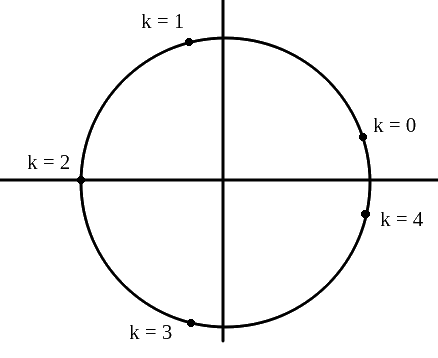
\includegraphics[scale=0.5]{sqrt_5_1}
    \caption{Расположение $ x_k $ на единичной окружности}
    \label{fig:1}
\end{figure}
Корни расположены как показано на рис. \ref{fig:1}. То есть $ \overline{x_4} = x_0, \overline{x_3} = x_1, x_2 = -1 $
$$ F'(x) = 5x^4, \qquad F'(x_k) = 5x_k^4 = 5x_k^{-1}x_k^5 = -5x_k^{-1} $$
При этом,
$$ x_k + \overline{x_k} = 2\operatorname{Re} x_k = 2\cos \frac{(2k + 1)\pi}5, \qquad x_k\overline{x_k} = |x_k|^2 = 1 $$
По формуле Лагранжа,
\begin{multline*}
    \frac1{x^5 + 1} = \sum_{k = 0}^4 \frac1{(x - x_k)(-5x_k^{-1})} = -\frac15 \sum \frac{x_k}{x - x_k} = -\frac15 \bigg( \frac{x_1}{x - x_1} + \frac{x_2}{x - x_2} + \frac{x_3}{x - x_3} + \frac{x_4}{x - x_4} \bigg) = \\
    = -\frac15 \bigg( \frac{x_1}{x - x_1} + \frac{\overline{x_1}}{x - \overline{x_1}} + \frac{x_3}{x - x_3} + \frac{\overline{x_3}}{x - \overline{x_3}} - \frac1{x + 1} \bigg) = \\
    = -\frac15 \bigg( \frac{x_1(x - \overline{x_1}) + \overline{x_1}(x - x_1)}{(x - x_1)(x - \overline{x_1})} + \frac{x_3(x - \overline{x_3}) + \overline{x_3}(x - x_3)}{(x - x_3)(x - \overline{x_3})} - \frac1{x + 1} \bigg) = \\
    = -\frac15 \bigg( \frac{x_1x - x_1\overline{x_1} + \overline{x_1}x - \overline{x_1}x_1}{x^2 - xx_1 - x\overline{x_1} + x_1\overline{x_1}} + \frac{x_3x - x_3\overline{x_3} + \overline{x_3}x - \overline{x_3}x_3}{x^2 - xx_3 - x\overline{x_3} + x_3\overline{x_3}} - \frac1{x + 1} \bigg) = \\
    = -\frac15 \bigg( \frac{x(x_1 + \overline{x_1}) - 2}{x^2 - x(x_1 + \overline{x_1}) + 1} + \frac{x(x_3 + \overline{x_3}) - 2}{x^2 - x(x_3 + \overline{x_3}) + 1} - \frac1{x + 1} \bigg) = \\
    = -\frac15 \bigg( \frac{2x\cos \frac{(2k + 1)\pi}5 - 2}{x^2 - 2x\cos \frac{(2k + 1)\pi}5 + 1} + \frac{2x\cos \frac{(2k + 1)\pi}5 - 2}{x^2 - 2x\cos \frac{(2k + 1)\pi}5 + 1} - \frac1{x + 1} ) = -\frac45 \frac{\cos \frac{(2k + 1)\pi}5x - 1}{x^2 - 2\cos \frac{(2k + 1)\pi}5x + 1} + \frac1{5(x + 1)}
\end{multline*}

\section{626}

\subsection{a}

$$ \frac1{x^3 - 1} = \frac1{(x - 1)(x^2 + x + 1)} = \frac{A}{x - 1} + \frac{Bx + C}{x^2 + x + 1} $$
$$ 1 = A(x^2 + x + 1) + (Bx + C)(x - 1) = Ax^2 + Ax + A + Bx^2 - Bx + Cx - C = (A + B)x^2 + (A - B + C)x + (A - C) $$
$$
\begin{cases}
	A + B = 0 \\
    A - B + C = 0 \\
    A - C = 1
\end{cases} \qquad
\begin{cases}
	A = -B \\
    C = A - 1 = -B - 1 \\
    -B - B - B - 1 = 0
\end{cases} \qquad
\begin{cases}
	B = -\frac13 \\
    C = -\frac23 \\
    A = \frac13
\end{cases} $$
$$ \frac1{3(x - 1)} - \frac{x + 2}{3(x^2 + x + 1)} $$

\subsection{b}

$$ \frac{x^2}{x^4 - 16} = \frac{x^2}{(x^2 - 4)(x^2 + 4)} = \frac{x^2}{(x - 2)(x + 2)(x^2 + 4)} = \frac{A}{x - 2} + \frac{B}{x + 2} + \frac{Cx + D}{x^2 + 4} $$
\begin{multline*}
    x^2 = A(x + 2)(x^2 + 4) + B(x - 2)(x^2 + 4) + (Cx + D)(x^2 - 4) = \\
    = Ax^3 + 2Ax^2 + 4Ax + 8A + Bx^3 - 2Bx^2 + 4Bx - 8B + Cx^3 - 4Cx + Dx^2 - 4D = \\
    = (A + B + C)x^3 + (2A - 2B + D)x^2 + (4A + 4B - 4C)x + (8A - 8B - 4D)
\end{multline*}
$$
\begin{cases}
	A + B + C = 0 \\
    2A - 2B + D = 1 \\
    A + B - C = 0 \\
    2A - 2B - D = 0
\end{cases} \qquad
\begin{cases}
	C = 0 \\
    A + B = 0 \\
    D = 1 - 2A + 2B \\
    2A - 2B - 1 + 2A - 2B = 0
\end{cases} \qquad
\begin{cases}
	A = -B \\
    D = 1 + 2B + 2B = 1 + 4B \\
    4A - 4B - 1 = 0
\end{cases} $$
$$ -B = B + \frac14 \qquad
\begin{cases}
	B = -\frac18 \\
    A = \frac18 \\
    D = 1 - \frac48 = \frac12 \\
    C = 0
\end{cases} $$
$$ \frac1{8(x - 2)} - \frac1{8(x + 2)} + \frac1{2(x^2 + 4)} $$

\subsection{c}

$$ \frac1{x^4 + 4} $$
Разложим над $ \Co $:
$$ 4 = 4(\cos 0 + i \sin 0) $$
Корни многочлена $ F(x) = x^4 + 4 $ имеют вид
$$ x_k = \sqrt2 \bigg( \cos \frac{2\pi k}4 + i \sin \frac{2\pi k}4 \bigg) = \sqrt2 \bigg( \cos \half[\pi k] + i\sin \half[\pi k] \bigg), \qquad k = 0, 1, 2, 3 $$
При этом,
\begin{itemize}
	\item $ x_0 = \sqrt2 $
    \item $ \overline{x_1} = x_3 $
    \item $ x_2 = -\sqrt2 $
    \item $ x_k + \ol{x_k} = 2 \operatorname{Re} x_k = 2\sqrt2 \cos \half[\pi k] $
    \item $ x_k\ol{x_k} = |x_k|^2 = 1 $
\end{itemize}
$$ F'(x) = 4x^3, \qquad F'(x_k) = 4x_k^3 = -4x_k^{-1} $$
По формуле Лагранжа,
\begin{multline*}
    \frac1{x^4 + 4} = \sum_{k = 0}^3 \frac1{(x - x_k)(-4x_k^{-1})} = -\frac14 \bigg\lgroup \frac{x_0}{x - x_0} + \frac{x_2}{x - x_2} + \frac{x_1}{x - x_1} + \frac{\ol{x_1}}{x - \ol{x_1}} \bigg\rgroup = \\
    = -\frac14 \bigg( \frac{\sqrt2}{x - \sqrt2} - \frac{\sqrt2}{x + \sqrt2} + \frac{x_1(x - \ol{x_1}) + \ol{x_1}(x - x_1)}{(x - x_1)(x - \ol{x_1})} \bigg) = -\frac14 \bigg( \frac{\sqrt2}{x - \sqrt2} - \frac{\sqrt2}{x + \sqrt2} + \frac{x(x_1 + \ol{x_1}) - 2x_1\ol{x_1}}{x^2 - x(x_1 + \ol{x_1}) + x_1\ol{x_1}} \bigg) = \\
    = -\frac14 \bigg( \frac{\sqrt2}{x - \sqrt2} - \frac{\sqrt2}{x + \sqrt2} + \frac{x \cdot 2\sqrt2\cos\half[\pi] - 2}{x^2 - x \cdot 2\sqrt2\cos\half[\pi] + 1} \bigg) = -\frac14 \bigg( \frac{\sqrt2}{x - \sqrt2} - \frac{\sqrt2}{x + \sqrt2} - \frac2{x^2 + 1} \bigg)
\end{multline*}

\subsection{d}

$$ \frac{x^2}{x^5 + 27} $$
Разложим над $ \Co $:
$$ -27 = 27(\cos \pi + i \sin \pi) $$
Корни многочлена $ F(x) = x^5 + 27 $ имеют вид
$$ x_k = 27^{\faktor15} \bigg( \cos \frac{(2k + 1)\pi}5 + i \sin \frac{(2k + 1)\pi}5 \bigg), \qquad k = 0, 1, ..., 4 $$
При этом,
\begin{itemize}
    \item $ x_0 = \overline{x_4} $
    \item $ x_1 = \overline{x_3} $
    \item $ x_2 = -\sqrt[5]{27} $
    \item $ x_k + \ol{x_k} = 2 \operatorname{Re} x_k = 2 \cdot 27^{\faktor15} \cos \frac{(2k + 1)\pi}5 $
    \item $ x_k\ol{x_k} = |x_k|^2 = 27^2 $
\end{itemize}
$$ F'(x) = 5x^4, \qquad F'(x_k) = 5x_k^4 = -27 \cdot 5 x_k^{-1} $$
$$ x_k^m = 27^{\faktor{m}5} \bigg( \cos \frac{(2k + 1)m\pi}5 + i \sin \frac{(2k + 1)m\pi}5 \bigg) $$
По формуле Лагранжа,
\begin{multline*}
    \frac{x^2}{x^5 + 27} = \sum_{k = 0}^4 \frac{x_k^2}{(x - x_k)(-27 \cdot 5 x_k^{-1})} = -\frac1{135} \bigg( \frac{x_2^3}{x - x_2} + \sum_{k = 0}^1 \frac{x_k^3}{x - x_k} + \sum_{k = 0}^1 \frac{\ol{x_k}^3}{x - \ol{x_k}} \bigg) = \\
    = -\frac1{135} \bigg( \frac{-27^{\faktor35}}{x - \sqrt[5]{27}} + \sum \frac{x_k^3(x - \ol{x_k}) + \ol{x_k}^3(x - x_k)}{(x - x_k)(x - \ol{x_k})} \bigg) = \\
    = -\frac1{135} \bigg( \frac{-27^{\faktor35}}{x - \sqrt[5]{27}} + \sum \frac{x(x_k^3 + \ol{x_k}^3) - x_k^2x_k\ol{x_k} - \ol{x_k}^2\ol{x_k}x_k}{x^2 - x(x_k + \ol{x_k}) + x_k\ol{x_k}} \bigg) = \\
    = -\frac1{135} \bigg( \frac{-27^{\faktor35}}{x - \sqrt[5]{27}} + \sum \frac{x \cdot 2 \cdot 27^{\faktor35} \cos \frac{(2k + 1)3\pi}5 - 27^2(x_k^2 + \ol{x_k}^2)}{x^2 - x \cdot 2 \cdot \sqrt[5]{27} \cos \frac{(2k + 1)\pi}5 + 27^2} \bigg) = \\
    = -\frac1{135} \bigg( \frac{-27^{\faktor35}}{x - \sqrt[5]{27}} + \sum \frac{x \cdot 2 \cdot 27^{\faktor35} \cos \frac{(2k + 1)3\pi}5 - 2 \cdot 27^{\faktor45} \cos \frac{(2k + 1)2\pi}5}{x^2 - x \cdot 2 \cdot \sqrt[5]{27} \cos \frac{(2k + 1)\pi}5 + 27^2} \bigg) = \\
    = \frac{27^{\faktor35}}{135} \bigg( \frac1{x - \sqrt[5]{27}} - 2\sum_{k = 0,1} \frac{x \cos \frac{(2k + 1)3\pi}5 - \sqrt[5]{27} \cos \frac{(2k + 1)2\pi}5}{x^2 - 2x\sqrt[5]{27} \cos \frac{(2k + 1)\pi}5 + 27^2} \bigg)
\end{multline*}

\subsection{e}

$$ \frac{x^m}{x^{2n +1} - 1}, \qquad m < 2n + 1 $$
Разложим над $ \Co $: \\
Корни многочлена $ F(x) = x^{2n + 1} - 1 $ имеют вид:
$$ x_k = \cos \frac{2\pi k}{2n + 1} + i \sin \frac{2\pi k}{2n + 1}, \qquad k = 0, 1, ..., 2n $$
Они разбиваются на пары сопряжённых: $ x_k $ при $ k = 1, 2, ..., n $, сопряжённые к ним и $ x_0 = 1 $
$$ F'(x) = (2n + 1)x^{2n}, \qquad F'(x_k) = (2n + 1)x_k^{2n} = (2n + 1)x_k^{-1} $$
$$ f(x_k) = x_k^m = \cos \frac{2\pi km}{2n + 1} + i \sin \frac{2\pi k m}{2n + 1} = x_{km} $$
По формуле Лагранжа,
\begin{multline*}
    \frac{x^m}{x^{2n + 1} - 1} = \frac{x_0^m}{(x - x_0)(2n + 1)x_0^{-1}} + \sum_{k = 1}^n \frac{x_k^m}{(x - x_k)(2n + 1)x_k^{-1}} + \sum_{k = 1}^n \frac{\overline{x_k}^m}{(x - \overline{x_k})(2n + 1)\overline{x_k}^{-1}} = \\
    = \frac1{2n + 1} \bigg\lgroup \frac1{x - 1} + \sum \bigg( \frac{x_k^{m + 1}}{x - x_k} + \frac{\overline{x_k}^{m + 1}}{x - \overline{x_k}} \bigg) \bigg\rgroup = \frac1{2n + 1} \bigg( \frac1{x - 1} + \sum \frac{x_{k(m + 1)}(x - \overline{x_k}) + \overline{x_{k(m + 1)}}(x - x_k)}{x^2 - xx_k - x\overline{x_k} + x_k\overline{x_k}} \bigg) = \\
    = \frac1{2n + 1} \bigg( \frac1{x - 1} + \sum \frac{x_{k(m + 1)}x - x_{k(m + 1)}\overline{x_k} + \overline{x_{k(m + 1)}}x - \overline{x_{k(m + 1)}}x_k}{x^2 - x(x_k + \overline{x_k}) + 1} \bigg) = \\
    = \frac1{2n + 1} \bigg( \frac1{x - 1} + \sum \frac{x(x_{k(m + 1)} + \overline{x_{k(m + 1)}}) - (x_{km}x_k\overline{x_k} + \overline{x_{km}}\overline{x_k}x_k)}{x^2 - 2x\cos \frac{2\pi k}{2n + 1} + 1} \bigg) = \\
    = \frac1{2n + 1} \bigg( \frac1{x - 1} + 2\sum \frac{x\cos \frac{2\pi k(m + 1)}{2n + 1} - \cos \frac{2\pi km}{2n + 1}}{x^2 - 2x \cos \frac{2\pi k}{2n + 1} + 1} \bigg)
\end{multline*}

\subsection{f}

$$ \frac{x^m}{x^{2n + 1} + 1}, \qquad m < 2n + 1 $$
Разложим над $ \Co $:
$$ -1 = \cos \pi + i \sin \pi $$
Корни многочлена $ F(x) = x^{2n + 1} + 1 $ имеют вид:
$$ x_k = \cos \frac{(2k + 1)\pi}{2n + 1} + i \sin \frac{(2k + 1)\pi}{2n + 1}, \qquad k = 0, 1, ..., 2n $$
Они разбиваются на:
\begin{itemize}
	\item $ x_k $ при $ k = 0, .., n - 1 $
    \item сопряжённые им
    \item $ x_n = -1 $
\end{itemize}
$$ F'(x) = (2n + 1)x^{2n}, \qquad F'(x_k) = -(2n + 1)x_k^{-1} $$
$$ x_k^m = \cos \frac{(2k + 1)m\pi}{2n + 1} + i \sin \frac{(2k + 1)m\pi}{2n + 1} $$
По формуле Лагранжа,
\begin{multline*}
    \frac{x^m}{x^{2n + 1} + 1} = \frac{x_n^m}{(x - x_n)(-(2n + 1)x_n^{-1})} + \sum_{k = 0}^{n - 1} \frac{x_k^m}{(x - x_k)(-(2n + 1)x_k^{-1})} + \sum_{k = 0}^{n - 1} \frac{\overline{x_k}^m}{(x - \overline{x_k})(-(2n + 1)\overline{x_k}^{-1})} = \\
    = -\frac1{2n + 1} \bigg\lgroup \frac{(-1)^{m + 1}}{x + 1} + \sum \bigg( \frac{x_k^{(m + 1)}}{x - x_k} + \frac{\overline{x_k}^{(m + 1)}}{x - \overline{x_k}} \bigg) \bigg\rgroup = \\
    = -\frac{(-1)^{m + 1}}{2n + 1} \bigg( \frac{(-1)^{m + 1}}{x + 1} + \sum \frac{x_k^{(m + 1)}(x - \overline{x_k}) + \overline{x_k}^{(m + 1)}(x - x_k)}{(x - x_k)(x - \overline{x_k})} \bigg) = \\
    = -\frac1{2n + 1} \bigg( \frac{(-1)^{m + 1}}{x + 1} + \sum \frac{x(x_k^{(m + 1)} + \overline{x_k}^{(m + 1)}) - (x_k^mx_k\overline{x_k} + \overline{x_k}^m\overline{x_k}x_k)}{x^2 - x(x_k + \overline{x_k}) + x_k\overline{x_k}} \bigg) = \\
    = -\frac1{2n + 1} \bigg( \frac{(-1)^{m + 1}}{x + 1} + \sum \frac{2x\cos \frac{(2k + 1)(m + 1)\pi}{2n + 1} - (x_k^m + \overline{x_k}^m)}{x^2 - 2x\cos \frac{(2k + 1)\pi}{2n + 1} + 1} \bigg) = \\
    = -\frac1{2n + 1} \bigg( \frac{(-1)^{m + 1}}{x + 1} + 2\sum \frac{x\cos \frac{(2k + 1)(m + 1)\pi}{2n + 1} - \cos \frac{(2k + 1)m\pi}{2n + 1}}{x^2 - 2x\cos \frac{(2k + 1)\pi}{2n + 1} + 1} \bigg)
\end{multline*}

\subsection{g}

$$ \frac1{x^{2n} - 1} $$
Над $ \Co $: \\
Корни многочлена $ F(x) = x^{2n} - 1 $ имеют вид
$$ x_k = \cos \frac{2\pi k}{2n} + i \sin \frac{2\pi k}{2n} = \cos \frac{\pi k}n + i \sin \frac{\pi k}n, \qquad k = 0, ..., 2n - 1 $$
Они разбиваются на $ x_k $ при $ k = 1, ..., n - 1 $, сопряжённые им $ \overline{x_k} = x_{2n - 1 - k} $, $ x_0 = 1 $ и $ x_n = -1 $
$$ F'(x) = 2nx^{2n - 1}, \qquad F'(x_k) = 2nx_k^{2n - 1} = 2nx_k^{-1} $$
По формуле Лагранжа,
\begin{multline*}
    \frac1{x^{2n} - 1} = \frac1{(x - x_0)(2nx_0^{-1})} + \frac1{(x - x_n)(2nx_n^{-1})} + \sum_{k = 1}^{n - 1} \frac1{(x - x_k)(2nx_k^{-1})} + \sum_{k = 0}^{n - 1} \frac1{(x - \overline{x_k})(2n\overline{x_k}^{-1})} = \\
    = \frac1{2n} \bigg\lgroup \frac{x_0}{x - x_0} + \frac{x_n}{x - x_n} + \sum \bigg( \frac{x_k}{x - x_k} + \frac{\overline{x_k}}{x - \overline{x_k}} \bigg) \bigg\rgroup = \\
    = \frac1{2n} \bigg\lgroup \frac1{x - 1} - \frac1{x + 1} + \sum \frac{x_k(x - \overline{x_k}) + \overline{x_k}(x - x_k)}{(x - x_k)(x - \overline{x_k})} \bigg\rgroup = \frac1{2n} \bigg\lgroup \frac1{x - 1} - \frac1{x + 1} + \sum \frac{x_kx - x_k\overline{x_k} + \overline{x_k}x - \overline{x_k}x_k}{x^2 - xx_k - x\overline{x_k} + x_k\overline{x_k}} \bigg\rgroup = \\
    = \frac1{2n} \bigg\lgroup \frac1{x - 1} - \frac1{x + 1} + \sum \frac{x(x_k + \overline{x_k}) - 2}{x^2 - x(x_k + \overline{x_k}) + 1} \bigg\rgroup = \frac1{2n} \bigg\lgroup \frac1{x - 1} - \frac1{x + 1} + \sum \frac{2x\cos \frac{\pi k}n - 2}{x^2 - 2x\cos \frac{\pi k}n + 1} \bigg\rgroup = \\
    = \frac1{2n} \bigg\lgroup \frac1{x - 1} - \frac1{x + 1} + 2\sum_{k = 0}^{n - 1} \frac{x\cos\frac{\pi k}n - 1}{x^2 - 2x\cos \frac{\pi k}n + 1} \bigg\rgroup
\end{multline*}

\subsection{h}

$$ \frac{x^{2m}}{x^{2n} + 1} $$
Разложим над $ \Co $:
$$ -1 = \cos \pi + i \sin \pi $$
Корни многочлена $ F(x) = x^{2n} + 1 $ имеют вид:
$$ x_k = \cos \frac{(2k + 1)\pi}{2n} + i \sin \frac{(2k + 1)\pi}{2n}, \qquad k = 0, ..., 2n - 1 $$
Они разбиваются на $ x_k $ при $ k = 0, ..., n - 1 $ и сопряжённые к ним
$$ F'(x) = 2nx^{2n - 1}, \qquad F'(x_k) = 2nx_k^{2n - 1} = -2nx_k^{-1} $$
$$ x_k^m = \cos \frac{(2k + 1)m\pi}{2n} + i \sin \frac{(2k + 1)\pi}{2n} $$
По формуле Лагранжа,
\begin{multline*}
    \frac{x^{2m}}{x^{2n} + 1} = \sum_{k = 0}^{n - 1} \frac{x_k^{2m}}{(x - x_k)(-2nx_k^{-1})} + \sum_{k = 0}^{n - 1} \frac{\overline{x_k}^{2m}}{(x - \overline{x_k})(-2n\overline{x_k}^{-1})} = -\frac1{2n} \sum \bigg( \frac{x_k^{2m + 1}}{x - x_k} + \frac{\overline{x_k}^{2m + 1}}{x - \overline{x_k}} \bigg) = \\
    = -\frac1{2n} \sum \frac{x_k^{2m + 1}(x - \overline{x_k}) + \overline{x_k}^{2m + 1}(x - x_k)}{(x - x_k)(x - \overline{x_k})} = -\frac1{2n} \sum \frac{x(x_k^{2m + 1} + \overline{x_k}^{2m + 1}) - (x_k^{2m}x_k\overline{x_k} + \overline{x_k}^{2m}\overline{x_k}x_k)}{x^2 - x(x_k + \overline{x_k}) + x_k\overline{x_k}} = \\
    = -\frac1{2n} \sum \frac{2x\cos \frac{(2k + 1)(2m + 1)\pi}{2n} - (x_k^{2m} + \overline{x_k}^{2m})}{x^2 - 2x\cos \frac{(2k + 1)\pi}{2n} + 1} = -\frac1{n} \sum_{k = 0}^{n - 1} \frac{x\cos \frac{(2k + 1)(2m + 1)\pi}{2n} - \cos \frac{(2k + 1)m\pi}{2n}}{x^2 - 2x\cos \frac{(2k + 1)\pi}{2n} + 1}
\end{multline*}

\subsection{i}

$$ P = \frac1{x(x^2 + 1)(x^2 + 4)...(x^2 + n^2)} $$
Разложим над $ \Co $:
$$ P = \frac1{(x - x_0)(x - x_1)(x + x_1)(x - x_2)(x + x_2)...(x - x_n)(x + x_n)}, \qquad x_k =
\begin{cases}
	\sqrt{-k^2} = ik, \qquad k > 0 \\
    0, \qquad k = 0
\end{cases} $$
Обозначим знаменатель за $ F(x) $ \\
Обозначим $ \prod = (x - x_0)(x + x_0)...(x - x_n)(x + x_n) $
\begin{multline*}
    F'(x) =  \\
    = 1 \cdot (x - x_1)(x + x_1)...(x - x_n)(x + x_n) + (x - x_0) \cdot 1 \cdot (x - x_1)...(x - x_n)(x + x_n) + \widedots[3em] + (x - x_0)(x - x_1)...(x - x_n) \cdot 1 = \\
    = \prod_{i \ne 0} + \sum_k \bigg\lgroup \prod_{i \ne k} \cdot (x + x_k) + \prod_{i \ne k} \cdot (x - x_k) \bigg\rgroup = \prod_{i \ne 0} + \sum_k \bigg\lgroup \prod_{i \ne k} \cdot (x + x_k + x - x_k) \bigg\rgroup = \\
    = \prod_{i \ne 0} + \sum_k \bigg\lgroup \prod_{i \ne k} \cdot 2\underbrace{x}_{x + x_0} \bigg\rgroup = \prod_{i \ne 0} + 2\sum_{k = 1}^n \prod_{i \ne k}
\end{multline*}
Все слагаемые, кроме $ k $-го, содержат $ x - x_k $ \\
Обозначим $ \prod^{(t)} = (x_t - x_0)(x_t + x_0)...(x_t - x_n)(x_t + x_n) $
$$ F'(x_0) = \prod_{i \ne 0}^{(0)} = (-x_1)x_1...(-x_n)x_n = (-1)^nx_1^2...x_n^2 = (-1)^n(-1^2)...(-n^2) = 1^2...n^2 = (n!)^2 $$
$$ F'(x_p) = 2 \prod_{i \ne p}^{(p)} = 2\prod_{t \ne p} \bigg( (ip - it)(ip + it) \bigg) = 2\prod_{t \ne p} \bigg( -(p - t)(p + t) \bigg) = (-1)^{n - 1} \cdot 2 \prod_{t \ne p} (p^2 - t^2) $$
По формуле Лагранжа,
\begin{multline*}
    P = \frac1{(x - x_0) \cdot \prod_{i \ne 0}}^{(0)} + \sum_{k = 1}^n \frac1{(x - x_k) \cdot 2\prod_{i \ne k}^{(k)}} + \sum_{k = 1}^n \frac1{(x + x_k) \cdot 2\prod_{i \ne k}^{(k)}} = \\
    = \frac1{(n!)^2x} + \sum \frac1{(-1)^{n - 1} \cdot 2\prod_{t \ne k} (k^2 - t^2)} \bigg( \frac1{x - x_k} + \frac1{x + x_k} \bigg) = \\
    = \frac1{(n!)^2x} + \half[(-1)^{n - 1}] \sum \frac1{\prod_{t \ne k}(k^2 - t^2)} \cdot \frac{x + x_k + x - x_k}{x^2 - x_k^2} = \frac1{(n!)^2x} + (-1)^{n - 1} \sum \frac1{\prod_{t \ne k}(k^2 - t^2)} \cdot \frac{x}{x^2 + k^2}
\end{multline*}

\section{628}

Пусть $ \vphi(x) = (x - x_1)(x - x_2)...(x - x_n) $. Выразить через $ \vphi(x) $ суммы:

\subsection{a}

$$ \sum \frac1{x - x_i} = \frac{(x - x_2)...(x - x_n) + (x - x_1)(x - x_3)...(x - x_n) + \widedots[3em] + (x - x_1)(x - x_2)...(x - x_{n - 1})}{(x - x_1)(x - x_2)...(x - x_n)} $$
$$ \vphi'(x) = \underbrace{(x - x_1)'}_{= 1}(x - x_2)...(x - x_n) + \widedots[5em] + (x - x_1)(x - x_2)...\underbrace{(x - x_n)'}_{= 1} $$
$$ \sum = \frac{\vphi'(x)}{\vphi(x)} $$

\subsection{b}

\begin{multline*}
    \sum \frac{x_i}{x - x_i} = \frac{x_1(x - x_2)...(x - x_n) + (x - x_1)x_2...(x - x_n) + \widedots[3em] + (x - x_1)...(x - x_{n - 1})x_n}{(x - x_1)(x - x_2)...(x - x_n)} = \\
    = \frac{\bigg( x_1\prod_{i \ne 1} + x_2\prod_{i \ne 2} + \widedots[3em] + x_n\prod_{i \ne n} - x\prod_{i \ne 1} - \widedots[3em] - x\prod_{i \ne n} \bigg) + x\prod_{i \ne 1} + \widedots[3em] + x\prod_{i \ne n}}{\vphi(x)} = \\
    = \frac{-\bigg(\overbrace{(x - x_1)\prod_{i \ne 1} + \widedots[3em] + (x - x_n)\prod_{i \ne n}}^n \bigg) + x(\prod_{i \ne 1} + ... + \prod_{i \ne n})}{\vphi(x)} = \frac{-n\vphi(x) + x\vphi'(x)}{\vphi(x)}
\end{multline*}

\subsection{c}

\begin{multline*}
    \sum \frac1{(x - x_i)^2} = \\
    = \frac{(x - x_2)^2...(x - x_n)^2 + (x - x_1)^2...(x - x_n)^2 + \widedots[4em] + (x - x_1)^2(x - x_2)^2...(x - x_{n - 1})^2}{(x - x_1)^2...(x - x_n)^2} = \\
    = \frac{\sum_t \bigg( \prod_{i \ne t} \bigg)^2}{\vphi^2(x)}
\end{multline*}
$$ (\vphi')^2(x) = \bigg( \prod_{i \ne 1} + ... + \prod_{i \ne n} \bigg)^2 = \sum_{k, p} \prod_{i \ne k}\prod_{i \ne j} = \sum_t \bigg( \prod_{i \ne t} \bigg)^2 + \sum_{k \ne p} \bigg\lgroup \bigg(\prod_{i \ne k, p}\bigg)^2(x - x_p)(x - x_k) \bigg\rgroup $$
$$ \vphi''(x) = \prod_{i \ne 1, 2} + ... + \prod_{i \ne 1, n} + \widedots[4em] + \prod_{i \ne n, 1} + ... + \prod_{i \ne n, n - 1} = \sum_{k \ne p} \prod_{i \ne k, p} $$
$$ \vphi(x)\vphi''(x) = \prod \cdot \sum_{k \ne p} \prod_{i \ne k,p} = \sum \bigg\lgroup \prod \prod_{i \ne k, p} \bigg\rgroup = \sum_{k \ne p} \bigg\lgroup \bigg( \prod_{i \ne k, p} \bigg)^2 (x - x_k)(x - x_p) \bigg\rgroup $$
$$ \sum = \frac{(\vphi')^2(x) - \vphi(x)\vphi''(x)}{\vphi^2(x)} $$

\chapter{ДЗ к пересдаче}

\section{Вычисление варианта}

$$ var = (numbers \mod 2) + 1 $$

\begin{tabular}{c c c c c c c c c c c c c c c}
	С & е & н & и & ч & е & н & к & о & в & & П & ё & т & р \\
    19 & 6 & 15 & 10 & 25 & 6 & 15 & 12 & 16 & 3 & & 17 & 7 & 20 & 18
\end{tabular}

$$ numbers = 19 + 6 + 15 + 10 + 25 + 6 + 15 + 12 + 16 + 3 + 17 + 7 + 20 + 18 = 189 $$
$$ numbers \mod 2 = 1 $$
$$ var = 1 + 1 = 2 $$

\section{1}

Привести к каноническому виду ортогональным преобразованием квадратичную форму

\subsection{1}

$$ Q = \sum_{i = 1}^n x_i^2 + \sum_{i < j}x_ix_j $$
$$ A =
\begin{pmatrix}
	1 & \half & . & \half \\
    \half & 1 & . & \half \\
    . & . & . & . \\
    \half & . & \half & 1
\end{pmatrix} $$
\begin{itemize}
	\item $ \lambda = \half $
    $$ A - \half I =
    \begin{pmatrix}
    	\half & ... & \half \\
        . & . & . \\
        \half & . & \half
    \end{pmatrix} $$
    $$ \dim \ker(A - \half I) = n - \rk(A - \half I) = n - 1 $$
    \item $ \sum \lambda_i = \operatorname{tr}A \implies \lambda = n - (n - 1) \cdot \half = \half[2n - n + 1] = \half[n + 1] $
\end{itemize}
$$ Q = \sum_{i = 1}^{n - 1} \half[x_i^2] + \half[(n + 1)x_n^2] $$

\subsection{2}

$$ \sum_{i < j} x_ix_j $$
$$ A =
\begin{pmatrix}
	0 & \half & . & \half \\
    \half & 0 & . & \half \\
    . & . & . & . \\
    \half & . & \half & 0
\end{pmatrix} $$
\begin{itemize}
	\item $ \lambda = -\half $
    $$ A + \half I =
    \begin{pmatrix}
    	\half & . & \half \\
        . & . & . \\
        \half & . & \half
    \end{pmatrix} $$
    $$ \dim \ker = n - \rk(A - \half I) = n - 1 $$
    \item $ \operatorname{tr} A = \sum \lambda_i $
    $$ \lambda = \operatorname{tr} A + (n - 1) \cdot \half = \half[n - 1] $$
\end{itemize}
$$ Q = -\sum_i^{n - 1} \half[x_i^2] + \half[(n - 1)x_n^2] $$

\section{2}

\subsection{1}

$$ \frac{x^3}{x^9 - 1} $$
Разложим над $ \Co $: \\
Корни многочлена $ F(x) = x^9 - 1 $ -- это корни из единицы девятой степени:
$$ x_k = \cos\frac{2\pi k}9 + i \sin\frac{2\pi k}9, \qquad k = 0, 1, ..., 8 $$
При этом, $ x_0 = 1 $, а остальные разбиваются на пары сопряжённых: $ \ol{x_k} = x_{9 - k} $
$$ F'(x) = 9x^8, \qquad F'(x_k) = 9x_k^8 = 9x_k^{-1} $$
По формуле Лагранжа,
\begin{multline*}
    \frac{x^3}{x^9 - 1} = \sum_{k = 0}^8 \frac{x_k^3}{(x - x_k)(9x_k^{-1})} = \frac19 \bigg\lgroup \frac{x_0^4}{x - x_0} + \sum_{k = 0}^8 \bigg( \frac{x_k^4}{x - x_k} + \frac{\ol{x_k}^4}{x - \ol{x_k}} \bigg) \bigg\rgroup = \\
    = \frac19 \bigg\lgroup \frac1{x - 1} + \sum \frac{x_k^4(x - \ol{x_k}) + \ol{x_k}^4(x - x_k)}{(x - x_k)(x - \ol{x_k})} \bigg\rgroup = \frac19 \bigg\lgroup \frac1{x - 1} + \sum \frac{x(x_k^4 + \ol{x_k}^4) - (x_k^3x_k\ol{x_k} + \ol{x_k}^3\ol{x_k}x_k)}{x^2 - x(x_k + \ol{x_k}) + x_k\ol{x_k}} \bigg\rgroup = \\
    = \frac19 \bigg\lgroup \frac1{x - 1} + \sum \frac{2x\cos\frac{8\pi k}9 - (x_k^3 + \ol{x_k}^3)}{x^2 - 2x\cos\frac{2\pi k}9 + 1} \bigg\rgroup = \frac19 \bigg\lgroup \frac1{x - 1} + \sum \frac{2x\cos\frac{8\pi k}9 - 2\cos\frac{6\pi k}9}{x^2 - 2x\cos\frac{2\pi k}9 + 1} \bigg\rgroup = \\
    = \frac19 \bigg\lgroup \frac1{x - 1} + 2\sum \frac{x\cos\frac{8\pi k}9 - \cos\frac{2\pi k}3}{x^2 - 2x\cos\frac{2\pi k}9 + 1} \bigg\rgroup
\end{multline*}

\subsection{2}

$$ \frac{x^3}{x^9 + 1} $$
Разложим над $ \Co $: \\
Корни многочлена $ F(x) = x^9 + 1 $ имеют вид
$$ x_k = \cos \frac{\pi + 2\pi k}9 + i \sin \frac{\pi + 2\pi k}9, \qquad k = 0, 1, ..., 8 $$
Они разбиваются на пары сопряжённых: $ \overline{x_k} = x_{8 - k} $, кроме $ x_4 = -1 $
$$ F'(x) = 9x^8, \qquad F'(x_k) = 9x_k^8 = 9\underbrace{x_k^9}_{= 1}x_k^{-1} = -9x_k^{-1} $$
$$ x_k + \overline{x_k} = 2\operatorname{Re}x_k = 2\cos \frac{(2k + 1)\pi}9, \qquad x_k\overline{x_k} = |x_k|^2 = 1, \qquad x_k^m = \cos \frac{(2k + 1)m\pi}9 + i \sin \frac{(2k + 1)m\pi}9 $$
По формуле Лагранжа,
\begin{multline*}
    \frac{x^3}{x^9 + 1} = \sum_{k = 0}^8 \frac{x_k^3}{(x - x_k)(-9x_k^{-1})} = -\frac19 \bigg\lgroup \sum_{k = 0}^3 \frac{x_k^4}{x - x_k} + \frac{x_4^4}{x - x_4} + \sum_{k = 0}^3 \frac{\overline{x_k}^4}{x - \overline{x_k}} \bigg\rgroup = \\
    = -\frac19 \bigg\lgroup \frac1{x + 1} + \sum_{k = 0}^3 \frac{x_k^4(x - \ol{x_k}) + \ol{x_k}^4(x - x_4)}{(x - x_k)(x - \ol{x_k})} \bigg\rgroup = -\frac19 \bigg\lgroup \frac1{x + 1} + \sum_{k = 0}^3 \frac{x(x_k^4 + \ol{x_k}^4) - x_k^3x_k\ol{x_k} - \ol{x_k}^3\ol{x_k}x_k}{x^2 - x(x_k + \ol{x_k}) + x_k\ol{x_k}} \bigg\rgroup = \\
    = -\frac19 \bigg\lgroup \frac1{x + 1} + \sum_{k = 0}^3 \frac{2x\cos\frac{(2k + 1)4\pi}9 - (x_k^3 + \ol{x_k}^3)}{x^2 - 2x\cos\frac{(2k + 1)\pi}9 + 1} \bigg\rgroup = -\frac19 \bigg\lgroup \frac1{x + 1} + 2\sum_{k = 0}^3 \frac{x\cos\frac{4(2k + 1)\pi}9 - \cos\frac{3(2k + 1)\pi}9}{x^2 - 2x\cos\frac{(2k + 1)\pi}9 + 1} \bigg\rgroup
\end{multline*}

\section{3}

\subsection{1}

\begin{statement}
	Пусть конечная группа $ G $ состоит из чётного числа элементов. Доказать, что существует элемент порядка 2
\end{statement}

\begin{proof}
	Каждый элемент в группе имеет обратный \\
    Единица обратная сама к себе, остальные разбиваются на пары обратных \\
    Значит, чтобы группа имела чётное число элементов, какой-то элемент (кроме 1) должен совпасть со своим обратным, то есть
    $$ a = a^{-1} \implies 1 = aa^{-1} = aa = a^2 \implies \ord(a) = 2 $$
\end{proof}

\subsection{2}

\begin{statement}
	Пусть группа $ G $ не имеет нетривиальных подгрупп. Доказать, что $ G $ конечна и $ |G| $ простое
\end{statement}

\begin{iproof}
    \item Докажем, что $ G $ конечна. Пусть это не так. \\
    Пусть $ C = \set{\braket{g} | g \in G} $ -- множество всех циклических подгрупп $ G $ \\
    Возможно два случая:
    \begin{itemize}
    	\item $ |C| = \infty \implies G $ содержит бесконечное число циклических подгрупп
        \item $ C $ -- конечно (некоторые из $ \braket{g} $ совпали) \\
        Пусть $ C = \set{H_1, H_2, ..., H_n} $ \\
        Хотя бы одна из них бесконечна, пусть это $ H_1 = \braket{g_1} $ \\
        Она изоморфна $ \Z $ и содержит бесконечное число циклических подгрупп \\
        Значит и $ G $ содержит бесконечное число циклических подгрупп
    \end{itemize}
    При этом, единственная тривиальная циклическая подгруппа -- $ \braket{e} $ -- \contra $ \implies G $ конечна
    \item Докажем, что $ |G| = p \in \Prime $ \\
    Пусть это не так, то есть $ |G| = n $, где $ n = pm $ \\
    Возьмём $ a \in G, \quad a \ne e \implies a^{pm} = e $ \\
    Рассмотрим два случая:
    \begin{itemize}
    	\item $ a^p \ne e $ \\
        Возьмём циклическую подгруппу $ H = \braket{a^p} $ \\
        $ 1 < |H| \le m < pm $ -- \contra
        \item $ a^p = e $ \\
        Возьмём циклическую подгурппу $ H = \braket{a} $ \\
        $ 1 < |H| \le p < pm $ -- \contra
    \end{itemize}
\end{iproof}

\section{4}

\subsection{1}

Пусть $ V = \R^4 $, $ W $ -- подпространство $ V $, натянутое на векторы $
\begin{pmatrix}
	1 \\
    1 \\
    1 \\
    2
\end{pmatrix},
\begin{pmatrix}
	1 \\
    0 \\
    -1 \\
    -1
\end{pmatrix} $, $ U $ -- подпространство $ V $, натянутое на векторы $
\begin{pmatrix}
	3 \\
    1 \\
    -1 \\
    0
\end{pmatrix},
\begin{pmatrix}
	3 \\
    3 \\
    2 \\
    2
\end{pmatrix} $. Найти размерность и базис для $ W \cap U $, $ W + U $. Является ли $ W + U $ прямой суммой?

\begin{itemize}
	\item $ W \cap U $ \\
    Возьмём $ v \in W \cap U $
    $$ v \in W \implies v = a
    \begin{pmatrix}
    	1 \\
        1 \\
        1 \\
        2
    \end{pmatrix} + b
    \begin{pmatrix}
    	1 \\
        0 \\
        -1 \\
        -1
    \end{pmatrix}, \qquad v \in U \implies v = c
    \begin{pmatrix}
    	3 \\
        1 \\
        -1 \\
        0
    \end{pmatrix} + d
    \begin{pmatrix}
    	3 \\
        3 \\
        2 \\
        2
    \end{pmatrix} $$
    $$
    \begin{cases}
    	a + b - 3c - 3d = 0 \\
        a - c - 3d = 0 \\
        a - b + c - 2d = 0 \\
        2a - b - 2d = 0
    \end{cases} \qquad
    \begin{cases}
    	a = c + 3d \\
        c + 3d - 3c - 3d = 0 \\
        c + 3d - b + c - 3d = 0 \\
        2c + 6d - b - 2d = 0
    \end{cases} \qquad
    \begin{cases}
    	-2c = 0 \\
        ...
    \end{cases} \qquad a = b = c = d = 0 $$
    $$ W \cap U = \set{0}, \qquad \dim(W \cap U) = 0 $$
    \item $ W + U $
    $$ W + U = \left\langle
    \begin{pmatrix}
    	1 \\
        1 \\
        1 \\
        2
    \end{pmatrix},
    \begin{pmatrix}
    	1 \\
        0 \\
        -1 \\
        -1
    \end{pmatrix},
    \begin{pmatrix}
    	3 \\
        1 \\
        -1 \\
        0
    \end{pmatrix},
    \begin{pmatrix}
    	3 \\
        3 \\
        2 \\
        2
    \end{pmatrix} \right\rangle $$
    $$ W \cap U = \set{0} \implies W \oplus U, \qquad \dim(W \cap U) = \dim V = 4 $$
    Значит, этот набор и является базисом
\end{itemize}

\subsection{2}

Пусть $ V = \R^4 $, $ W $ -- подпространство $ V $, натянутое на векторы $
\begin{pmatrix}
	0 \\
    1 \\
    -1 \\
    1
\end{pmatrix},
\begin{pmatrix}
	-1 \\
    -2 \\
    2 \\
    2
\end{pmatrix} $, $ U $ -- подпространство $ V $, натянутое на векторы $
\begin{pmatrix}
	-1 \\
    1 \\
    -1 \\
    5
\end{pmatrix},
\begin{pmatrix}
	3 \\
    3 \\
    2 \\
    1
\end{pmatrix} $ \\
Найти размерность и базис для $ W \cap U $ и $ W + U $. Является ли $ W + U $ прямой суммой?
\begin{itemize}
	\item $ W \cap U $ \\
    Возьмём $ v \in W \cap U $
    $$ v \in W \implies v = a
    \begin{pmatrix}
    	0 \\
        1 \\
        -1 \\
        1
    \end{pmatrix} + b
    \begin{pmatrix}
    	-1 \\
        -2 \\
        2 \\
        2
    \end{pmatrix}, \qquad v \in U \implies v = c
    \begin{pmatrix}
    	-1 \\
        1 \\
        -1 \\
        5
    \end{pmatrix} + d
    \begin{pmatrix}
    	3 \\
        3 \\
        2 \\
        1
    \end{pmatrix} $$
    $$
    \begin{cases}
    	-b + c - 3d = 0 \\
        a - 2b - c - 3d = 0 \\
        -a + 2b + c - 2d = 0 \\
        a + 2b - 5c - d = 0
    \end{cases} \qquad
    \begin{cases}
    	b = c - 3d \\
        a - 2c + 6d - c - 3d = 0 \\
        -a + 2c - 6d + c - 2d = 0 \\
        a + 2c - 6d - 5c - d = 0
    \end{cases} \qquad
    \begin{cases}
    	a - 3c + 3d = 0 \\
        -a + 3c - 8d = 0 \\
        a - 3c - 7d = 0
    \end{cases} $$
    $$
    \begin{cases}
    	a = 3c - 3d \\
        -3c + 3d + 3c - 8d = 0 \\
        3c - 3d - 3c - 7d = 0
    \end{cases} \qquad
    \begin{cases}
    	-5d = 0 \\
        -10d = 0
    \end{cases} \qquad a = b = c = d = 0 $$
    $$ W \cap U = \set{0}, \qquad \dim(W \cap U) = 0 $$
    \item $ W + U $
    $$ W + U = \left\langle
    \begin{pmatrix}
    	0 \\
        1 \\
        -1 \\
        1
    \end{pmatrix},
    \begin{pmatrix}
    	-1 \\
        -2 \\
        2 \\
        2
    \end{pmatrix},
    \begin{pmatrix}
    	-1 \\
        1 \\
        -1 \\
        5
    \end{pmatrix},
    \begin{pmatrix}
    	3 \\
        3 \\
        2 \\
        1
    \end{pmatrix} \right\rangle $$
    $$ W \cap U = \set{0} \implies W \oplus U \implies \dim(W + U) = 4 $$
    Значит, этот набор будет базисом
\end{itemize}

\section{ДЗ к пересдаче. Дубль 2}

\subsection{Квадратичные формы}

\subsubsection{1}

$$ Q = \sum_{i = 1}^n x_i^2 + \sum_{i < j}x_ix_j $$
$$ A =
\begin{pmatrix}
	1 & \half & . & . & \half \\
    \half & 1 & \half & . & \half \\
    . & . & . & . & . \\
    \half & . & . & \half & 1
\end{pmatrix} $$
$$ \chi(\lambda) =
\begin{vmatrix}
	1 - \lambda & \half & . & \half \\
    \half & 1 - \lambda & . & \half \\
    . & . & . & . \\
    \half & . & \half & 1 - \lambda
\end{vmatrix} $$
\begin{itemize}
	\item $ \lambda = \half $
    $$ A - \half I =
    \begin{pmatrix}
    	\half & . & \half \\
        . & . & . \\
        \half & . & \half
    \end{pmatrix} $$
    Ранг этой матрицы равен 1. Значит, размерность ядра равна $ n - 1 $
    \item $ \sum \lambda_i = \operatorname{tr} A = n $
    $$ \lambda = n - (n - 1) \cdot \half = \half[n + 1] $$
\end{itemize}
$$ Q = \sum_i^{n - 1} \half[x_i]^2 + \half[(n + 1)x_n^2] $$

\subsection{2}

$$ Q = \sum_{i < j} x_ix_j $$
$$ A =
\begin{pmatrix}
	0 & \half & . & \half \\
    \half & 0 & . & \half \\
    . & . & . & . \\
    \half & . & \half & 0
\end{pmatrix} $$
\begin{itemize}
	\item $ \lambda = -\half $
    $$ A + \half I =
    \begin{pmatrix}
    	\half & . & \half \\
        . & . & . \\
        \half & . & \half
    \end{pmatrix} $$
    Ранг этой матрицы равен 1, значит, размерность ядра равна $ n - 1 $
    \item $ \sum \lambda_i = \operatorname{tr} A = 0 $
    $$ \lambda = \half[n - 1] $$
\end{itemize}
$$ Q = -\sum_{i = 1}^{n - 1} \half[x_i^2] + \half[(n - 1)x_n^2] $$

\section{Разложение на простейшие}

\subsection{1}

$$ \frac{x^3}{x^9 - 1} $$
Разложим над $ \Co $: \\
Корни многочлена $ F(x) = x^9 - 1 $ -- это корни из единицы 9 степени:
$$ x_k = \cos \frac{2\pi k}9 + i \sin \frac{2 \pi k}9, \qquad k = 0, ..., 8 $$
При этом, $ x_0 = 1 $, а остальные разбиваются на пары сопряжённых: $ \ol{x_k} = x_{9 - k} $
$$ F'(x) = 9x^8, \qquad F'(x_k) = 9x_k^8 = 9x_k^9x_k^{-1} = 9x_k^{-1} $$
$$ x_k + \ol{x_k} = 2\operatorname{Re}x_k = 2\cos \frac{2\pi k}9, \qquad x_k\ol{x_k} = |x_k|^2 = 1, \qquad x_k^m = \cos\frac{2\pi k m}9 + i \sin \frac{2\pi km}9 $$
Воспользуемся формулой Лагранжа:
\begin{multline*}
    \frac{x^3}{x^9 - 1} = \sum_{k = 0}^8 \frac{x_k^3}{(x - x_k)(9x_k^{-1})} = \frac19 \bigg\lgroup \frac{x_0^4}{x - x_0} + \sum_{k = 1}^4 \frac{x_k^4}{x - x_k} + \sum_{k = 1}^4 \frac{\ol{x_k}^4}{x - \ol{x_k}} \bigg\rgroup = \\
    = \frac19 \bigg\lgroup \frac1{x - 1} + \sum_{k = 1}^4 \frac{x_k^4(x - \ol{x_k}) + \ol{x_k}^4(x - x_k)}{(x - x_k)(x - \ol{x_k})} \bigg\rgroup = \frac19 \bigg\lgroup \frac1{x - 1} + \sum_{k = 1}^4 \frac{x(x_k^4 + \ol{x_k}^4) - (x_k^3x_k\ol{x_k} + \ol{x_k}^3\ol{x_k}x_k)}{x^2 - x(x_k + \ol{x_k}) + x_k\ol{x_k}} \bigg\rgroup = \\
    = \frac19 \bigg\lgroup \frac1{x - 1} + \sum_{k = 1}^4 \frac{2x\cos\frac{8\pi k}9 - (x_k^3 + \ol{x_k}^3)}{x^2 - 2x\cos\frac{2\pi k}9 + 1} \bigg\rgroup = \frac19 \bigg\lgroup \frac1{x - 1} + 2\sum_{k = 1}^4 \frac{x\cos\frac{8\pi k}9 - \cos\frac{2\pi k}3}{x^2 - 2x\cos\frac{2\pi k}9 + 1} \bigg\rgroup
\end{multline*}

\subsection{2}

$$ \frac{x^3}{x^9 + 1} $$
Разложим над $ \Co $: \\
Корни многочлена $ F(x) = x^9 + 1 $ имеют вид
$$ x_k = \cos\frac{(2k + 1)\pi}9 + i\sin\frac{(2k + 1)\pi}9, \qquad k = 0, ..., 8 $$
При этом, $ x_4 = -1 $, а остальные разбиваются на пары сопряжённых: $ \ol{x_k} = x_{9 - k} $
$$ F'(x) = 9x^8, \qquad F'(x_k) = 9x_k^8 = 9x_k^9x_k^{-1} = -9x_k^{-1} $$
Воспользуемся формулой Лагранжа:
\begin{multline*}
    \frac{x^3}{x^9 + 1} = \sum_{k = 0}^8\frac{x_k^3}{(x - x_k)(-9x_k^{-1})} = -\frac19 \bigg\lgroup \frac1{x + 1} + \sum_{k = 0}^3 \frac{x_k^4(x - \ol{x_k}) + \ol{x_k}^4(x - x_k)}{(x - x_k)(x - \ol{x_k})} \bigg\rgroup = \\
    = -\frac19 \bigg\lgroup \frac1{x + 1} + \sum_{k = 0}^3 \frac{x(x_k^4 + \ol{x_k}^4) - (x_k^3 + \ol{x_k}^3)}{x^2 - 2x\cos\frac{(2k + 1)\pi}9 + 1} \bigg\rgroup = -\frac19 \bigg\lgroup \frac1{x + 1} + 2\sum_{k = 0}^3 \frac{x\cos\frac{4(2k + 1)\pi}9 - \cos\frac{(2k + 1)\pi}3}{x^2 - 2x\cos\frac{(2k + 1)\pi}9 + 1} \bigg\rgroup
\end{multline*}

\section{Теория групп}

\subsection{1}

\begin{statement}
	Пусть конечная группа $ G $ состоит из чётного числа элементов. Доказать, что существует элемент порядка 2
\end{statement}

\begin{proof}
	Каждый элемент группы имеет обратный, при этом обратный к единице -- это единица. Значит, все элементы, единицы, разбиваются на пары обратных. \\
    Чтобы группа содержала чётное число элементов, должен быть ещё один элемент, обратный сам к себе, т. е. $ \exist a \ne e : \quad a^{-1} = a \iff aa^{-1} = e \iff a^2 = e \iff \ord(a) = 2 $
\end{proof}

\subsection{2}

\begin{statement}
	Пусть группа $ G $ не имеет нетривиальных подгрупп. Доказать, что $ G $ конечна и $ |G| $ простое
\end{statement}

\begin{iproof}
	\item Докажем, что $ G $ циклическая: \\
    Пусть это не так. Тогда порождающее множество $ G $ состоит из нескольких элементов. Возьмём из него $ a \ne b $ \\
    Рассмотрим циклические подгруппы $ \braket{a} $ и $ \braket{b} $. Они не равны (т. к. $ a \not\in \braket{b} $ и наоборот). Значит, хотя бы одна из них нетривиальна -- \contra
    \item Докажем, что $ G $ конечна: \\
    $ G $ циклическая $ \implies G \sim
    \begin{cases}
        \Z, \qquad G \text{ бесконечна} \\
        \Z_n, \qquad n = \ord G < \infty
    \end{cases} $ \\
    $ \Z $ содержит нетривиальные подгруппы, значит $ G $ конечна и изоморфна $ \Z_n $
    \item Докажем, что $ n \in \Prime $: \\
    Пусть это не так, и $ n = mp $ \\
    Зафиксируем элемент $ a \in G $, $ a \ne e $. Тогда $ a^{pm} = e $. Возможно два случая:
    \begin{itemize}
    	\item $ a^p = e $ \\
        Рассмотрим циклическую подгруппу $ \braket{a} $
        $$ 1 < \ord(\braket{a}) \le p < mp \implies \braket{a} \text{ нетривиальна} $$
        \item $ a^p \ne e $ \\
        Рассмотрим циклическую подгруппу $ \braket{a^p} $
        $$ 1 < \ord{\braket{a^p}} \le m < mp \implies \braket{a^p} \text{ нетривиальна} $$
    \end{itemize}
    В обоих случаях получили противоречие, значит, $ n \in \Prime $
\end{iproof}

\section{Базисы подпространств}

subsection{1}

Пусть $ V = \R^4 $, $ W $ -- подпространство $ V $, натянутое на векторы
$$
\begin{pmatrix}
	1 \\
    1 \\
    1 \\
    2
\end{pmatrix},
\begin{pmatrix}
	1 \\
    0 \\
    -1 \\
    -1
\end{pmatrix} $$
$ U $ -- подпространство $ V $, натянутое на векторы
$$
\begin{pmatrix}
	3 \\
    1 \\
    -1 \\
    0
\end{pmatrix},
\begin{pmatrix}
	3 \\
    3 \\
    2 \\
    2
\end{pmatrix} $$
Найти размерность и базис для $ W \cap U $ и $ W + U $. Является ли $ W + U $ прямой суммой?

\begin{itemize}
	\item $ W \cap U $ \\
    Возьмём $ v \in U \cap W $
    $$ v \in W \implies v = a
    \begin{pmatrix}
    	1 \\
        1 \\
        1 \\
        2
    \end{pmatrix} + b
    \begin{pmatrix}
    	1 \\
        0 \\
        -1 \\
        -1
    \end{pmatrix}, \qquad v \in U \implies v = c
    \begin{pmatrix}
    	3 \\
        1 \\
        -1 \\
        0
    \end{pmatrix} + d
    \begin{pmatrix}
    	3 \\
        3 \\
        2 \\
        2
    \end{pmatrix} $$
    $$
    \begin{cases}
    	a + b - 3c - 3d = 0 \\
        a - c - 3d = 0 \\
        a - b + c - 2d = 0 \\
        2a - b - 2d = 0
    \end{cases} \qquad
    \begin{cases}
    	a = c + 3d \\
        c + 3d + b - 3c - 3d = 0 \\
        c + 3d - b + c - 2d = 0 \\
        2c - 6d - b - 2d = 0
    \end{cases} \qquad
    \begin{cases}
    	b - 2c = 0 \\
        -b + 2c + d = 0 \\
        -b + 2c - 8d = 0
    \end{cases} $$
    $$
    \begin{cases}
    	b = 2c \\
        -2c + 2c + d = 0 \\
        -2c + 2c - 8d = 0
    \end{cases} \qquad
    \begin{cases}
    	a = c \\
        b = 2c \\
        d = 0
    \end{cases} $$
    $$ U \cap W = \left\langle
    \begin{pmatrix}
    	1 \\
        2 \\
        1 \\
        0
    \end{pmatrix} \right\rangle, \qquad \dim (W \cap U) = 1 $$
    \item $ W + U $ \\
    $ \dim (W \cap U) \ne 0 \implies $ сумма не прямая
    $$ W \cap U = \left\langle
    \begin{pmatrix}
    	1 \\
        1 \\
        1 \\
        2
    \end{pmatrix},
    \begin{pmatrix}
    	1 \\
        0 \\
        -1 \\
        -1
    \end{pmatrix},
    \begin{pmatrix}
    	3 \\
        1 \\
        -1 \\
        0
    \end{pmatrix},
    \begin{pmatrix}
    	3 \\
        3 \\
        2 \\
        2
    \end{pmatrix} \right\rangle $$
    По формуле Грассмана, $ \dim (U + W) = \dim U + \dim W - \dim (U \cap W) = 3 $ \\
    Значит, нужно исключить один вектор
    $$
    \begin{cases}
    	a + b + 3c = 3 \\
        a + c = 3 \\
        a - b - c = 2 \\
        2a - b = 2
    \end{cases} \qquad
    \begin{cases}
    	a = 3 - c \\
        3 - c + b + 3c - 3 = 0 \\
        3 - c - b - c - 2 = 0 \\
        6 - 2c - b - 2 = 0
    \end{cases} \qquad
    \begin{cases}
    	b + 2c = 0 \\
        -b - 2c + 1 = 0 \\
        -b - 2c + 4 = 0
    \end{cases} \qquad b = -2c $$
    Четвёртый вектор выражается через остальные, значит его можно исключить. Базис $ U + W $:
    $$
    \begin{pmatrix}
    	1 \\
        1 \\
        1 \\
        2
    \end{pmatrix},
    \begin{pmatrix}
    	1 \\
        0 \\
        -1 \\
        -1
    \end{pmatrix},
    \begin{pmatrix}
        3 \\
        1 \\
        -1 \\
        0
    \end{pmatrix} $$
\end{itemize}

\subsection{2}

Пусть $ V = \R^4 $, $ W $ -- подпространство $ V $, натянутое на векторы
$$
\begin{pmatrix}
	0 \\
    1 \\
    -1 \\
    1
\end{pmatrix},
\begin{pmatrix}
	-1 \\
    -2 \\
    2 \\
    2
\end{pmatrix} $$
$ U $ -- подпространство $ V $, натянутое на векторы
$$
\begin{pmatrix}
	-1 \\
    1 \\
    -1 \\
    5
\end{pmatrix},
\begin{pmatrix}
	3 \\
    3 \\
    2 \\
    1
\end{pmatrix} $$
Найти размерность и базис для $ W \cap U $ и $ W + U $. Является ли $ W + U $ прямой суммой?

\begin{itemize}
	\item $ W \cap U $ \\
    Возьмём $ v \in W \cap U $
    $$ v \in W \implies v = a
    \begin{pmatrix}
    	0 \\
        1 \\
        -1 \\
        1
    \end{pmatrix} + b
    \begin{pmatrix}
    	-1 \\
        -2 \\
        2 \\
        2
    \end{pmatrix}, \qquad v \in U \implies v = c
    \begin{pmatrix}
    	-1 \\
        1 \\
        -1 \\
        5
    \end{pmatrix} + d
    \begin{pmatrix}
    	3 \\
        3 \\
        2 \\
        1
    \end{pmatrix} $$
    $$
    \begin{cases}
    	-b + c - 3d = 0 \\
        a - 2b - c - 3d = 0 \\
        -a + 2b + c - 2d = 0 \\
        a + 2b - 5c - d = 0
    \end{cases} \qquad
    \begin{cases}
    	b = c - 3d \\
        a - 2c + 6d - c - 3d = 0 \\
        -a + 2c - 6d + c - 2d = 0 \\
        a + 2c - 6d - 5c - d = 0
    \end{cases} \qquad
    \begin{cases}
    	b = c - 3d \\
        a - 3c + 3d = 0 \\
        -a + 3c - 8d = 0 \\
        a - 3c - 7d = 0
    \end{cases} $$
    $$
    \begin{cases}
    	a = 3c - 3d \\
        -3c + 3d + 3c - 8d = 0 \\
        3c - 3d - 3c - 7d = 0
    \end{cases} \qquad
    \begin{cases}
    	a = 3c \\
        b = c \\
        d = 0
    \end{cases} $$
    $$ W \cap U = \left\langle
    \begin{pmatrix}
    	3 \\
        1 \\
        1 \\
        0
    \end{pmatrix} \right\rangle, \qquad \dim (W \cap U) = 1 $$
    \item $ W + U $ \\
    $ \dim(W \cap U) \ne 0 \implies $ сумма не прямая \\
    По формуле Грассмана,
    $$ \dim(W + U) = \dim U + \dim W - \dim(W \cap U) = 3 $$
    $$ W + U = \left\langle
    \begin{pmatrix}
    	0 \\
        1 \\
        -1 \\
        1
    \end{pmatrix},
    \begin{pmatrix}
    	-1 \\
        -2 \\
        2 \\
        2
    \end{pmatrix},
    \begin{pmatrix}
    	-1 \\
        1 \\
        -1 \\
        5
    \end{pmatrix},
    \begin{pmatrix}
    	3 \\
        3 \\
        2 \\
        1
    \end{pmatrix} \right\rangle $$
    Базис должен состоять из трёх векторов, значит один ветор надо исключить
    $$
    \begin{cases}
    	-a - b + 3c = 0 \\
        -2a + b + 3c = 1 \\
        2a - b + 2c = -1 \\
        2a + 5b + c = 1
    \end{cases} \qquad
    \begin{cases}
    	a = -b + 3c \\
        2b - 6c + b + 3c = 1 \\
        -2b + 6c - b + 2c = - 1 \\
        -2b + 6c + 5b + c = 1
    \end{cases} \qquad
    \begin{cases}
    	3b - 3c - 1 = 0 \\
        -3b + 8c + 1 = 0 \\
        3b + 7c - 1 = 0
    \end{cases} $$
    $$
    \begin{cases}
    	a = -\frac13 \\
        b = \frac13 \\
        c = 0
    \end{cases} $$
    Первый вектор выражается через остальные. Базис $ W + U $:
    $$
    \begin{pmatrix}
    	-1 \\
        -2 \\
        2 \\
        2
    \end{pmatrix},
    \begin{pmatrix}
    	-1 \\
        1 \\
        -1 \\
        5
    \end{pmatrix},
    \begin{pmatrix}
    	3 \\
        3 \\
        2 \\
        1
    \end{pmatrix} $$
\end{itemize}
